% ***************************************************
% A Classic Thesis Style
% An Homage to The Elements of Typographic Style
%
% Copyright (C) 2012 Andr\'e Miede http://www.miede.de
%
% If you like the style then I would appreciate a postcard. My
% address can be found in the file ClassicThesis.pdf. A collection
% of the postcards I received so far is available online at 
% http://postcards.miede.de
%
% License:
% This program is free software; you can redistribute it and/or
% modify it under the terms of the GNU General Public License as
% published by the Free Software Foundation; either version 2 of
% the License, or (at your option) any later version.
%
% This program is distributed in the hope that it will be useful,
% but WITHOUT ANY WARRANTY; without even the implied warranty of
% MERCHANTABILITY or FITNESS FOR A PARTICULAR PURPOSE.  See the
% GNU General Public License for more details.
%
% You should have received a copy of the GNU General Public
% License along with this program; see the file COPYING.  If not,
% write to the Free Software Foundation, Inc., 59 Temple Place -
% Suite 330, Boston, MA 02111-1307, USA.
%
% ***************************************************************
% Note:
%    * You must not use "u etc. in strings/commands that will be spaced out (use \"u or real umlauts instead)
%    * New enumeration (small caps): \begin{aenumerate} \end{aenumerate}
%    * For margin notes: \marginpar or \graffito{}
%    * Do not use bold fonts in this style, it is designed around them
%    * Use tables as in the examples
%    * See classicthesis-preamble.sty for useful commands
% ****************************************************************

\documentclass[ %twoside, 
			openright,
			% letterpaper a4paper
			titlepage, 
			numbers=noenddot,
			headinclude, %1headlines
            		footinclude=true, 
			cleardoublepage=empty,
			abstractoff, % <--- obsolete, remove (todo)
			BCOR=5mm,
			paper=a4, 
			fontsize=11pt, %11pt,
			]{scrreprt}

%*****************************************************************
% Note: Make all your adjustments in here
%*****************************************************************

% \usepackage[backref, backend=biber]{biblatex}
\usepackage{bibentry}
\usepackage[backref,
		backend=bibtex,
            	maxbibnames=99,
            	natbib=true,
            	firstinits=false,
            	%style=authoryear-comp,
            	sortcites=false,
            	doi=false,
            	url=false]{biblatex}
\usepackage{lettrine}

%\bibliographystyle{ACM-Reference-Format}
\bibliography{Bibliography}	

%\input{classicthesis-config}
% ****************************************************************
% classicthesis-config.tex 
% formerly known as loadpackages.sty, classicthesis-ldpkg.sty, and
% classicthesis-preamble.sty Use it at the beginning of your
% ClassicThesis.tex, or as a LaTeX Preamble in your
% ClassicThesis.{tex,lyx} with \input{classicthesis-config}
% ****************************************************************
% If you like the classicthesis, then I would appreciate a
% postcard. My address can be found in the file
% ClassicThesis.pdf. A collection of the postcards I received so
% far is available online at http://postcards.miede.de
% ****************************************************************

% ****************************************************************
% 1. Configure classicthesis for your needs here, e.g., remove
% "drafting" below in order to deactivate the time-stamp on the
% pages
% ****************************************************************
\PassOptionsToPackage{eulerchapternumbers,
					listings,
					%drafting,
				 	pdfspacing,
					floatperchapter,
					%linedheaders,
				 	subfig,
					beramono,
					eulermath,
					parts}{classicthesis}										

% ****************************************************************
% Triggers for this config
% **************************************************************** 
\usepackage{ifthen}
\newboolean{enable-backrefs} % enable backrefs in the bibliography
\setboolean{enable-backrefs}{false} % true false
% TODO backref is incompatible?
% ****************************************************************


% ****************************************************************
% 2. Personal data and user ad-hoc commands
% ****************************************************************
\newcommand{\myTitle}{Using Symbolic Execution to Improve the Runtime Management of Spark Applications\xspace}
\newcommand{\myTitleIT}{Un modello per tesi di laurea magistrale al DEIB \xspace}
\newcommand{\myFirstAuthorName}{Davide Bertolotti\xspace}
\newcommand{\myMatrFirstAuthor}{787366\xspace}
% \newcommand{\mySecondAuthorName}{Emanuele Mason\xspace}
% \newcommand{\myMatrSecondAuthor}{222222\xspace}
\newcommand{\mySupervisor}{Prof. Luciano Baresi\xspace} % relatore
\newcommand{\myOtherSupervisor}{Dr. Giovanni Quattrocchi\xspace} % co relatori
%\newcommand{\myOtherOtherSupervisor}{Prof. my ASP supervisor\xspace}
%\newcommand{\myCoExaminer}{Prof. Rodolfo Soncini-Sessa\xspace} % contro-relatore
\newcommand{\myFaculty}{Facolt\`a di Ingegneria\xspace}
\newcommand{\mySchool}{Scuola di Ingegneria Industriale e dell’Informazione\xspace}
\newcommand{\myDepartment}{Dipartimento di Elettronica, Informazione e Bioingegneria\xspace}
\newcommand{\myCourseFirstPart}{Master of Science in\xspace}
%\newcommand{\myCourseFirstPartIT}{Corso di Laurea Magistrale in\xspace}
\newcommand{\myCourseSecondPart}{Computer Science and Engineering\xspace}
%\newcommand{\myCourseSecondPartIT}{Ingegneria per l'Ambiente e il Territorio\xspace}
\newcommand{\myUni}{Politecnico di Milano\xspace}
\newcommand{\myLocation}{Milan\xspace}
\newcommand{\myTime}{April 2018\xspace}
\newcommand{\myVersion}{version 1.0\xspace}
\newcommand{\myAcademicYear}{Academic Year 2017-2018\xspace}
%\newcommand{\myAcademicYearIT}{Anno Accademico 2011-2012\xspace}

% ********************************************************************
% Setup, fine tuning, and useful commands
% ********************************************************************
\newcounter{dummy} % necessary for correct hyperlinks (to index, bib, etc.)
\newlength{\abcd} % for ab..z string length calculation
\providecommand{\mLyX}{L\kern-.1667em\lower.25em\hbox{Y}\kern-.125emX\@}
% from here till the end of the section, you can modify whatever you want
\newcommand{\ie}{i.\,e.\ }
\newcommand{\Ie}{I.\,e.\ }
\newcommand{\eg}{e.\,g.\ }
\newcommand{\Eg}{E.\,g.\ }
% referencing commands
\newcommand{\myEq}[1]{equation \eqref{#1}}
\newcommand{\MyEq}[1]{Equation \eqref{#1}}
\newcommand{\myFig}[1]{figure \ref{#1}}
\newcommand{\MyFig}[1]{Figure \ref{#1}}
\newcommand{\myListing}[1]{listing \ref{#1}}
\newcommand{\MyListing}[1]{Listing \ref{#1}}
\newcommand{\myTab}[1]{table \ref{#1}}
\newcommand{\MyTab}[1]{Table \ref{#1}}
\newcommand{\mySubsec}[1]{subsection \ref{#1}}
\newcommand{\MySubsec}[1]{Subsection \ref{#1}}
\newcommand{\mySec}[1]{section \ref{#1}}
\newcommand{\MySec}[1]{Section \ref{#1}}
\newcommand{\myChap}[1]{chapter \ref{#1}}
\newcommand{\MyChap}[1]{Chapter \ref{#1}}
\newcommand{\myAppendix}[1]{appendix \ref{#1}}
\newcommand{\MyAppendix}[1]{Appendix \ref{#1}}
\newcommand{\myEmph}[1]{\textsc{#1}}
\newcommand{\stwoe}{\text{S\textsuperscript{2}E}}


% **********************************************************************
% Imports from articolo Symbolic Execution
% **********************************************************************
\newcommand\cSpark{xSpark\xspace}
\newcommand\dSymb{\textit{SEEPEP}\xspace}
\newcommand\tool{\textit{xSpark$_{SEEPEP}$}\xspace}

\newcommand\plan{\textit{PEP}\xspace}
\newcommand\plans{\textit{PEPs}\xspace}

\newcommand{\approach}{SEEPEP\xspace}
\newcommand{\model}{PEP*\xspace}
\newcommand{\sparsedata}{SDD\xspace}
\newcommand\qos{\textit{QoS}\xspace}
\usepackage{adjustbox}
\usepackage{array}
\usepackage{booktabs}
\usepackage{multirow}
\newcolumntype{R}[2]{%
	>{\adjustbox{angle=#1,lap=\width-(#2)}\bgroup}%
	l%
	<{\egroup}%
}
%\newcommand*\rot{\multicolumn{1}{R{90}{1em}}}
%\newcommand*\rot{\multicolumn{1}{R{90}{1em}{|}}}
% **********************************************************************


% **********************************************************************
% 3. Loading some handy packages
% **********************************************************************
\PassOptionsToPackage{T1}{fontenc} % T2A for cyrillics
	\usepackage{fontenc} 
\PassOptionsToPackage{utf8}{inputenc} % latin9 (ISO-8859-9) = latin1+"Euro sign"
	\usepackage{inputenc}				
%\PassOptionsToPackage{utf8x}{inputenc} % ∞ char & others
%\usepackage{inputenc}				

\PassOptionsToPackage{autostyle,italian=guillemets,threshold=2}{csquotes}
 	\usepackage{csquotes}

\PassOptionsToPackage{american,italian}{babel}
	 \usepackage{babel}

\usepackage{textcomp} % fix warning with missing font shapes
\usepackage{scrhack} % fix warnings when using KOMA with listings package          
\usepackage{xspace} % to get the spacing after macros right  
\usepackage{mparhack} % get marginpar right
\usepackage{fixltx2e} % fixes some LaTeX stuff
\usepackage{microtype}
\usepackage[normalem]{ulem} % to have strikethrough text

\PassOptionsToPackage{printonlyused,smaller}{acronym}
	\usepackage{acronym} % nice macros for handling all acronyms in the thesis
% **********************************************************************

%*********************************************************************************
% 3.a Math
%*********************************************************************************
\PassOptionsToPackage{fleqn}{amsmath} % math environments and more by the AMS 
 	\usepackage{amsmath}
 
\usepackage{amsthm}
\usepackage{amssymb}
\renewcommand\qedsymbol{$\blacksquare$}

\theoremstyle{definition}
\newtheorem{definition}{Definition}[chapter]
\newtheorem{theorem}{Theorem}[chapter]

\theoremstyle{plain}
\newtheorem{observation}[definition]{Observation}
\newtheorem{corollary}[theorem]{Corollary}
\newtheorem{lemma}[theorem]{Lemma}
% **********************************************************************


% **********************************************************************
% 4. Setup floats: tables, (sub)figures, and captions
% **********************************************************************
\usepackage{tabularx} % better tables
	\setlength{\extrarowheight}{3pt} % increase table row height
\newcommand{\tableheadline}[2]{\multicolumn{1}{#1}{\normalsize\spacedlowsmallcaps{#2}}}
\newcommand{\tableheadlineMore}[3]{\multicolumn{#1}{#2}{\normalsize\spacedlowsmallcaps{#3}}}
\newcommand{\tablefirstcol}[2]{\multicolumn{1}{#1}{\textbf{#2}}}

\usepackage{caption}
	\captionsetup{format=hang,labelfont={sf,bf},font=small}
\usepackage{colortbl}
\usepackage{multirow}

\usepackage{subfig}
%\usepackage{subcaption}
\usepackage{fancyvrb}
\usepackage{siunitx}
\usepackage{paralist}
\usepackage{stmaryrd}
% *********************************************************************


% *********************************************************************
% 5. Setup code listings
% *********************************************************************
\usepackage{listings}
\lstloadlanguages{bash, C++, Java, Matlab, Scala, Python, C}

% for special keywords
\lstset{language=[LaTeX]Tex,
    keywordstyle=\color{RoyalBlue},%\bfseries,
    basicstyle=\small\ttfamily,
    %identifierstyle=\color{NavyBlue},
    commentstyle=\color{Green}\ttfamily,
    stringstyle=\rmfamily,
    numbers=none,%left,%
    numberstyle=\scriptsize,%\tiny
    stepnumber=5,
    numbersep=8pt,
    showstringspaces=false,
    breaklines=true,
    frameround=ftff,
    frame=single,
    belowcaptionskip=.75\baselineskip
    %frame=L
} 
% *********************************************************************


% *********************************************************************
% 6. PDFLaTeX, hyperreferences and citation backreferences
% *********************************************************************
% ********************************************************************
% Using PDFLaTeX
% ********************************************************************
\PassOptionsToPackage{pdftex,hyperfootnotes=false,pdfpagelabels}{hyperref}
	\usepackage{hyperref}  % backref linktocpage pagebackref
\pdfcompresslevel=9
\pdfadjustspacing=1 
\PassOptionsToPackage{pdftex}{graphicx}
	\usepackage{graphicx} 

% ********************************************************************
% Setup the style of the backrefs from the bibliography
% (translate the options to any language you use)
% ********************************************************************
\newcommand{\backrefnotcitedstring}{\relax}%(Not cited.)
\newcommand{\backrefcitedsinglestring}[1]{(Cited on page~#1.)}
\newcommand{\backrefcitedmultistring}[1]{(Cited on pages~#1.)}
\ifthenelse{\boolean{enable-backrefs}}%
{%
		\PassOptionsToPackage{hyperpageref}{backref}
		\usepackage{backref} % to be loaded after hyperref package 
		   \renewcommand{\backreftwosep}{ and~} % separate 2 pages
		   \renewcommand{\backreflastsep}{, and~} % separate last of longer list
		   \renewcommand*{\backref}[1]{}  % disable standard
		   \renewcommand*{\backrefalt}[4]{% detailed backref
		      \ifcase #1 %
		         \backrefnotcitedstring%
		      \or%
		         \backrefcitedsinglestring{#2}%
		      \else%
		         \backrefcitedmultistring{#2}%
		      \fi}%
}{\relax}    


% ****************************************************************
% PDF/A compliance
% ****************************************************************
% TODO not working: requires downloading color specification file in a specific
% tex folder and other hacks I don't want to spend time with
% \usepackage[a-1b]{pdfx}

% ********************************************************************
% Hyperreferences
% ********************************************************************
\hypersetup{%
    %draft,	% = no hyperlinking at all (useful in b/w printouts)
    colorlinks=true, linktocpage=true, pdfstartpage=3, pdfstartview=FitV,%
    % uncomment the following line if you want to have black links (e.g., for printing)
    %colorlinks=false, linktocpage=false, pdfborder={0 0 0}, pdfstartpage=3, pdfstartview=FitV,% 
    breaklinks=true, pdfpagemode=UseNone, pageanchor=true, pdfpagemode=UseOutlines,%
    plainpages=false, bookmarksnumbered, bookmarksopen=true, bookmarksopenlevel=1,%
    hypertexnames=true, pdfhighlight=/O,%nesting=true,%frenchlinks,%
    urlcolor=webbrown, linkcolor=RoyalBlue, citecolor=webgreen, 
    %pagecolor=RoyalBlue,%
    %urlcolor=Black, linkcolor=Black, citecolor=Black, %pagecolor=Black,%
} 

    %pdftitle={\myTitle},%
    %pdfauthor={\textcopyright\ \myFirstAuthorName and \mySecondAuthorName, \myUni, \myFaculty},%
    %pdfsubject={},%
    %pdfkeywords={},%
    %pdfcreator={pdfLaTeX},%
    %pdfproducer={LaTeX with hyperref and classicthesis}%

%}   

% ********************************************************************
% Setup autoreferences
% ********************************************************************
% There are some issues regarding autorefnames
% http://www.ureader.de/msg/136221647.aspx
% http://www.tex.ac.uk/cgi-bin/texfaq2html?label=latexwords
% you have to redefine the makros for the 
% language you use, e.g., american, ngerman
% (as chosen when loading babel/AtBeginDocument)
% ********************************************************************
\makeatletter
\@ifpackageloaded{babel}%
    {%
       \addto\extrasamerican{%
					\renewcommand*{\figureautorefname}{Figure}%
					\renewcommand*{\tableautorefname}{Table}%
					\renewcommand*{\partautorefname}{Part}%
					\renewcommand*{\chapterautorefname}{Chapter}%
					\renewcommand*{\sectionautorefname}{Section}%
					\renewcommand*{\subsectionautorefname}{Section}%
					\renewcommand*{\subsubsectionautorefname}{Section}% 	
				}%
       \addto\extrasitalian{% 
					\renewcommand*{\paragraphautorefname}{Paragrafo}%
					\renewcommand*{\subparagraphautorefname}{Paragrafo}%
					\renewcommand*{\footnoteautorefname}{Nota a pié di pagina}%
					\renewcommand*{\FancyVerbLineautorefname}{Zeile}%
					\renewcommand*{\theoremautorefname}{Teorema}%
					\renewcommand*{\appendixautorefname}{Appendice}%
					\renewcommand*{\equationautorefname}{Equazione}%        
					\renewcommand*{\itemautorefname}{Punto}%
				}%	
			% Fix to getting autorefs for subfigures right (thanks to Belinda Vogt for changing the definition)
			\providecommand{\subfigureautorefname}{\figureautorefname}%  			
    }{\relax}
\makeatother

% ****************************************************************
% 7. Last calls before the bar closes
% ****************************************************************

\usepackage{classicthesis} 
\usepackage[hcentering, 
			margin=4.4cm,%]{geometry}
			bindingoffset=4mm
			]{geometry}
% ****************************************************************

%*****************************************************************
% Hyphenation
%*****************************************************************
\hyphenation{put-here-the-words-latex-cannot-hyphenate}

\begin{document}

	% initial, local settings
	\numberwithin{equation}{chapter}
	\frenchspacing
	\raggedbottom
	\selectlanguage{american} % american/italian
	\pagenumbering{roman}
	\pagestyle{plain}
	
	%*************************************************************
	% Frontmatter
	%*************************************************************

	% Uncomment the following line to add the ''copertina'' to the pdf
	% \include{FrontBackmatter/Copertina}
	%*******************************************************
% Titlepage
%   the file is named in italian since our language 
%   provide different words for different things and
%   we should use them
%*******************************************************
\begin{titlepage}
	% if you want the titlepage to be centered, uncomment and
	% fine-tune the line below (KOMA classes environment)
	% \begin{addmargin}[-1cm]{-3cm}
    \begin{center}
    	\large
        \spacedlowsmallcaps{\myUni} \\
        \bigskip\myFaculty \\
        \medskip\mySchool \\
    	\medskip\myDepartment \\
    	\bigskip\myCourseFirstPart \\
        \medskip\myCourseSecondPart \\  

        \hfill

        \vfill
        
        \begin{figure}[!h]
			\begin{center}
				
\includegraphics[width=0.3\columnwidth]{Images/logo_polimi.png}%logoPoli.pdf} 
			\end{center}
		\end{figure}
		
		\vfill

        \begingroup
       		\huge	
            \color{Maroon} \myTitle
            \bigskip
        \endgroup

        \vfill

		\flushleft 
		\normalsize{Supervisor:}\\
		\medskip\spacedlowsmallcaps{\mySupervisor}

		\flushleft
		%\normalsize{Assistant Supervisor:}\\
		\normalsize{Co-Supervisor:}\\
		\medskip\spacedlowsmallcaps{\myOtherSupervisor}\\
		%comment if there is another supervisor
		%\flushleft
		%\normalsize{Alta Scuola Politecnica Assistant Supervisors:}\\
		%\medskip\spacedlowsmallcaps{\myOtherOtherSupervisor}\\
        
        \vfill  
        
        \flushright
        \normalsize{Master Graduation Thesis by:}\\
        \medskip \spacedlowsmallcaps{\myFirstAuthorName}\\
		Student Id n. \myMatrFirstAuthor \\ 
		% comment if there isn't any second author
		%\medskip\spacedlowsmallcaps{\mySecondAuthorName} \\
		%Student Id n. \myMatrSecondAuthor \\
		
		\vfill 

		\centering {\myAcademicYear}                     

    \end{center}  
  %\end{addmargin}       
\end{titlepage}
	% %*******************************************************
% Titlepage
%   the file is named in italian since our language 
%   provide different words for different things and
%   we should use them
%*******************************************************
\begin{titlepage}
	% if you want the titlepage to be centered, uncomment and fine-tune the line below (KOMA classes environment)
	% \begin{addmargin}[-1cm]{-3cm}
    \begin{center}
    	\large
        \spacedlowsmallcaps{\myUni} \\
        \bigskip\myFaculty \\
        \medskip\mySchool \\
    	\medskip\myDepartment \\
    	\bigskip\myCourseFirstPartIT \\
        \medskip\myCourseSecondPartIT \\  

        \hfill

        \vfill
        
        \begin{figure}[!h]
			\begin{center}
				
\includegraphics[width=0.3\columnwidth]{Images/logoPoli.pdf}
			\end{center}
		\end{figure}
		
		\vfill

        \begingroup
       		\huge	
            \color{Maroon} \myTitleIT \\ \bigskip
        \endgroup

        \vfill

		\flushleft 
		\normalsize{Relatore:}\\
		\medskip\spacedlowsmallcaps{\mySupervisor}

		\flushleft
		\normalsize{Correlatore:}\\
		\medskip\spacedlowsmallcaps{\myOtherSupervisor}\\
		%comment if there isn't any other supervisor
		%\flushleft
		%\normalsize{Correlatore Alta Scuola Politecnica:}\\
		%\medskip\spacedlowsmallcaps{\myOtherOtherSupervisor}\\
        
        \vfill  
        
        \flushright
        \normalsize{Tesi di Laurea Magistrale di:}\\
        \medskip \spacedlowsmallcaps{\myFirstAuthorName}\\
		Matricola n. \myMatrFirstAuthor \\ 
		% comment if there isn't any second author
		\medskip\spacedlowsmallcaps{\mySecondAuthorName} \\
		Matricola n. \myMatrSecondAuthor \\
		
		\vfill 

		\centering {\myAcademicYearIT}                     

    \end{center}  
  %\end{addmargin}       
\end{titlepage}
	%\thispagestyle{empty}

\hfill

\vfill

\pdfbookmark[0]{Colophon}{colophon}
\section*{Colophon}
This document was typeset using the typographical look-and-feel \texttt{classicthesis} developed by Andr\'e Miede.
The style was inspired by Robert Bringhurst's seminal book on typography ``\emph{The Elements of Typographic Style}''.
\texttt{classicthesis} is available for both \LaTeX\ and \mLyX: 
\begin{center}
\url{http://code.google.com/p/classicthesis/}
\end{center}
Happy users of \texttt{classicthesis} usually send a real postcard to the author, a collection of postcards received so far is featured here:
\begin{center}
\url{http://postcards.miede.de/}
\end{center}
The template has been adapted by Emanuele Mason, Andrea Cominola and Daniela Anghileri:
\textit{A template for master thesis at DEIB},
June 2015
 
\bigskip

\medskip

\noindent\finalVersionString % a.k.a. the colophon
	\cleardoublepage%*******************************************************
% Dedication
%*******************************************************
\thispagestyle{empty}
%\phantomsection 
\refstepcounter{dummy}
\pdfbookmark[1]{Dedication}{Dedication}

\vspace*{3cm}
\begin{center}
    Here you can put your dedication, like: \\ \medskip
    To time, that do not go backwards \\ \medskip
    --- A \& D \& E 
\end{center}
	% \cleardoublepage\include{FrontBackmatter/Publication}
	\cleardoublepage%*******************************************************
% Acknowledgments
%*******************************************************
\pdfbookmark[1]{Acknowledgments}{acknowledgments}

\bigskip

\begingroup
\let\clearpage\relax
\let\cleardoublepage\relax
\let\cleardoublepage\relax
\chapter*{Acknowledgments}
Here you can put acknowledgements to people that helped you during the thesis. Remember that helping students to write thesis is part of the job of some of them, and they're also paid for that. Please make sure to thank them for what they weren't supposed to do.

Remember also that this page is part of your thesis. I know that your boyfriend/girlfriend is very important to you and you cannot live without her/him, as it is for me. But there's no need to put her/his name here unless she/he gave a proper contribution to this work. Same goes for friends, parents, drinking buddies and so on.

\endgroup
	\cleardoublepage%*******************************************************
% Table of Contents
%*******************************************************
%\phantomsection
\refstepcounter{dummy}
\pdfbookmark[1]{\contentsname}{tableofcontents}
\setcounter{tocdepth}{2} % <-- 2 includes up to subsections in the ToC
\setcounter{secnumdepth}{3} % <-- 3 numbers up to subsubsections
\manualmark
\markboth{\spacedlowsmallcaps{\contentsname}}{\spacedlowsmallcaps{\contentsname}}
\tableofcontents 
\automark[section]{chapter}
\renewcommand{\chaptermark}[1]{\markboth{\spacedlowsmallcaps{#1}}{\spacedlowsmallcaps{#1}}}
\renewcommand{\sectionmark}[1]{\markright{\thesection\enspace\spacedlowsmallcaps{#1}}}
%*******************************************************
% List of Figures and of the Tables
%*******************************************************
\clearpage

\begingroup 
    \let\clearpage\relax
    \let\cleardoublepage\relax
    \let\cleardoublepage\relax
    %*******************************************************
    % List of Figures
    %*******************************************************    
    %\phantomsection 
    \refstepcounter{dummy}
    %\addcontentsline{toc}{chapter}{\listfigurename}
    \pdfbookmark[1]{\listfigurename}{lof}
    \listoffigures

    \vspace*{8ex}

    %*******************************************************
    % List of Tables
    %*******************************************************
    %\phantomsection 
    \refstepcounter{dummy}
    %\addcontentsline{toc}{chapter}{\listtablename}
    \pdfbookmark[1]{\listtablename}{lot}
    \listoftables
        
    \vspace*{8ex}
%   \newpage
    
    %*******************************************************
    % List of Listings
    %*******************************************************      
	  %\phantomsection 
    \refstepcounter{dummy}
    %\addcontentsline{toc}{chapter}{\lstlistlistingname}
    \pdfbookmark[1]{\lstlistlistingname}{lol}
    \lstlistoflistings 

    \vspace*{8ex}
       
    %*******************************************************
    % Acronyms
    %*******************************************************
    %\phantomsection 
    \refstepcounter{dummy}
    \pdfbookmark[1]{Acronyms}{acronyms}
    \markboth{\spacedlowsmallcaps{Acronyms}}{\spacedlowsmallcaps{Acronyms}}
    \chapter*{Acronyms}
	    % environment acronym take the longest acronym as parameter to
    % determine the wideness of columns. Put it between square bracket
    \begin{acronym}[EMODPS]
    	% put here the acronyms you use and recall them in text by
    	% using \ac{NAME}. In the text you can also use \acs{}, \acf{}, \acl{}
    	% for various flavours
	\acro{EMODPS}{Evolutionary Multi-Objective Direct Policy Search}
    	\acro{OS}{operating system}
         \acro{XML}{eXtensible Markup Language}
    \end{acronym}                  
\endgroup

\cleardoublepage
	\cleardoublepage%*******************************************************
% Abstract
%*******************************************************
%\renewcommand{\abstractname}{Abstract}
\addcontentsline{toc}{chapter}{\abstractname}

\pdfbookmark[1]{Abstract}{Abstract}
\begingroup
\let\clearpage\relax
\let\cleardoublepage\relax
\let\cleardoublepage\relax

\chapter*{Abstract}
\lettrine[lines=4]{\textcolor{purple}{T}}{he} need to crunch a steadily growing amount of data generated by the modern applications is driving an increasing demand of flexible computing power, that is more and more often satisfied by cloud computing solutions. Cloud computing  revolutionized the way computer infrastructures are abstracted and used by exploiting virtualization and providing an easy access to resources through the Internet~\cite{articleBigData:2017}.
%It is built on virtual hardware and software infrastructures accessible via the Internet and its usage is suitable for big data processing by enterprises of any size. 


Big data is a research field that deals with ways to analyze and extract information from data sets containing structured and unstructured data whose size is so large that makes the processing of data with traditional databases and applications very difficult or practically impossible. The processing of these data therefore requires the use of distributed frameworks specialized for the parallel execution of programs, such as Apache Hadoop~\cite{misc:ApacheHadoop} and Apache Spark~\cite{misc:ApacheSpark}. These specialized frameworks are used to transform the applications in atomic parts that can be executed in a distributed cluster of physical or virtual machines. 

%The limit to the level of parallelism that can be obtained is given by the number of machines and the amount of synchronization needed between the data fragments representing the intermediate results. 
Hadoop uses the Map-Reduce programming model that was firstly introduced by Google~\cite{misc:GoogleMapReduce} and consists of two distinct phases: Map and Reduce. %As suggested by the name, the reducer phase takes place after the mapper phase has been completed. 
%A map job reads and processes a block of data to produce key-value pairs as intermediate outputs, that are input to the reducer. The reducer receives the key-value pair from multiple map jobs and then aggregates those intermediate data tuples (intermediate key-value pair) into a smaller set of tuples or key-value pairs which is the final output.
The former processes and \textit{transforms} a block of data to produce key-value pairs (tuples) as intermediate outputs, the latter \textit{aggregates} these tuples into a final output.
%One of the most frequently used cluster computing frameworks for big data analytics is Apache Spark (Spark), which provides a fast and general, fault-tolerant data processing platform that allows quick in memory computation. Spark computation is based on RDDs, a data abstraction, and DAGs, representing the data manipulation processes.%

A more advanced solution is represented by Apache Spark~\cite{misc:ApacheSpark}, that allows for faster executions by avoiding or limiting the use of the persistent storage and it provides a more sophisticated programming model based on parallel execution plans (\plans) which are represented as directed acyclic graph (DAG) of phases.

%Spark uses a data abstraction called Resilient Distributed Dataset (RDD). 
%When an application is submitted to Spark, an application’s driver process is created to collect the results of the computations made on the RDDs, and the application is divided in multiple jobs. Jobs are delimited by Spark actions in the application code. Spark actions are  operations that return a value to the driver program after running a computation on an RDD.
%Spark applications consist of multiple jobs, that are delimited by Spark actions in the application code. For each job, a DAG or \textit{Parallel Execution Plan} (\plan), is created to keep track of the RDDs and maximize the parallelism while executing an application. 
%that are materialized inside the job. 
%DAG nodes represent the RDDs, meanwhile arcs represent transformations, that are the operations that create new datasets from existing ones. The application steps inside a single job are further organized into stages.
%, that are delimited by operations that require data reshuffling. The DAG defines the execution order among stages, and the extent to which stages can be executed in parallel. For each job, Spark computes a DAG or \textit{Parallel Execution Plan}, from now on called \plan to maximize the parallelism while executing an application. 
%The parallel execution plan of the application is obtained by joining the \plans of its job.
%Spark generalizes the two stage Map-Reduce to support arbitrary \plans, and provides fast data sharing between operations by executing in-memory computing, unlike Hadoop that requires intermediate data to be written to disk in order to be accessible by the following operations.
%The main advantage of Spark with respect to previous cluster computing frameworks is the fast data sharing between operations. For example, Apache Hadoop requires intermediate data to be written to disk in order to be accessible by the following operations, Spark instead allows to execute in-memory computing. 
Big data applications pose new challenges in satisfying requirements on the \textit{Quality of Service} (\qos) provided to end users. In the context of traditional applications (e.g. web) this problem has often been faced using self-adaptive systems that control runtime \textit{KPIs} (Key Performance Indicators) against changes in the application context and workload. %In the world of big data, the notion of \qos differ by application type. While interactive applications are usually assessed according to response time or throughput, 
%and their fulfillment depends on the intensity and variety of the incoming requests, 

Compared to traditional applications, where a single execution lasts ten to hundreds of milliseconds, big data applications might require minutes or hours to process large datasets, thus \qos must consider the execution of single runs. Therefore, in this domain the \qos is often defined by means of \textbf{deadline}s, that are the maximum allowed duration of as single application execution. %Thus, users may be interested in quantifying and constraining the execution time of \textit{\textbf{every single run}} of an application. 
%Cluster computing, an implementation of the Parallel Computing paradigm composed by a large number of networked multi-cpu computers in the cloud, is widely used to speed-up application execution time. 
%Clusters of networked multi-cpu computers in the cloud, implementing the Parallel Computing paradigm, are often used to speed-up the execution of big data applications. However, a fast 
%A fast computing system alone is not enough to guarantee that a big data application will meet a fixed deadline, as the execution time depends on many variable factors such as the amount of computing resources available (cpu's, memory, storage). Since the amount of work to execute the application is not known a priori and the deadline is fixed, the system must be able to allocate resources dynamically to the application at runtime to help meeting the \qos.
 
The execution time of big-data applications depends on many factors such as the amount of computing resources available (cpu's, memory, storage) and the concurrent execution of other applications on the same cluster. Therefore, in the literature one can find several approaches \cite{Verma2011, Hindman2011, Cheng2015} that focus on resource allocation or scheduling techniques in order to reduce deadline violations by using different techniques such as integer linear programming, machine learning and control theory.  %A fast computing system alone is not enough to guarantee that a big data application will meet a fixed deadline, as the execution time depends on many variable factors such as the amount of computing resources available (cpu's, memory, storage). Since the amount of work to execute the application is not known a priori and the deadline is fixed, the system must be able to allocate resources dynamically to the application at runtime to help meeting the \qos.

%The speed of execution of a big data application in fact depends on many factors that vary over time, such as the amount of resources available (i.e. number of cpu cores, amount of memory, storage space) or the amount of data to be processed. Since the amount of work required by the big data application is not known a priori and the deadline is fixed, the system must be capable of allocating the needed amount of resources dynamically at runtime (i.e. when they are required by the application) to meet the \qos. 
%

All of these approaches use the knowledge of the \plan to reason, predict or estimate the application execution time and work under the assumption that the application \plan does not change under different input datasets or application parameters. Unfortunately, this is true only if the application code does not contain any conditional branch whose outcome depends on user input values or the result of previous calculations involving input data. %If the  condition of uniqueness of the application \plan is violated, xSpark
Otherwise, different application \plans could be needed to describe all the possible execution flows generated by the combinations of all the different branch outcomes in the application code. Without considering all these \plans the analysis of the application could be significantly unprecise.


xSpark, developed at Politecnico di Milano, is an extension of the Apache Spark framework that offers fine-grained dynamic resource allocation using lightweight containers and control-theoretical planners. It allows users to set application deadlines (which is not possible using Spark) and uses the knowledge of the application \plan, retrieved during a profiling phase, to dynamically allocate resources to the application.
xSpark does not consider loops or conditional branches in the application code and assumes that the \plan is unique.

 %, composed by a centralized heuristic and a distributed local controller.
%Here is where \tool, the project described in this thesis, comes into play. 
\tool, the solution described in this thesis, extends xSpark capability to safely run multi-\plan applications, by exploiting symbolic execution. At each decisional branch outcome in the application, \tool determines which \plans are still valid and prunes the \plans tree, removing the invalid \plans, thus leaving only the valid ones in the \plans tree. A heuristic is used to select the \plan to execute among the valid ones, in order to minimize the risk of missing the deadline while maximizing the CPU usage efficiency.


%\paragraph{Results}
%The solution presented in this thesis is \tool, a toolchain providing the capability to manage the efficient execution of deadline-based QoS constrained multi-\plan Spark applications. \tool is the result of the integration of \dSymb, a tool exploiting symbolic execution techniques to generate the path condition associated to each possible {\plan}s produced by different inputs and parameters, with (a modified version of) xSpark. Moreover, \tool generates a launcher with a synthesized dataset for each \plan and \textit{GuardEvaluator}, an artifact that retrieves the feasible {\plan}s given a set of symbolic variables resolved to a value. Finally, we integrated this approach with xSpark, an extension of Spark that can control the duration of Spark applications according to specified deadlines through dynamic resource allocation. 
\tool is the result of the integration of \dSymb, a tool exploiting symbolic execution to discover all possible application {\plan}s produced by different inputs and parameters, with (a modified version of) xSpark.
%We tested \tool with two applications, Promocalls, that was developed at Politecnico di Milano in the Deib Labs\footnote{\url{https://github.com/seepep/promocalls}}, a paradigmatic application resembling a daily routine of a telecommunications company for calculating the application of promotional discounts to the most active users, and Louvain, a Spark implementation of the Louvain algorithm~\cite{Louvain} that we downloaded from a highly ranked GitHub repository\footnote{\url{https://github.com/Sotera/spark-distributed-louvain-modularity}}. Louvain uses \textit{GraphX}, a Spark library specialized for graph processing, suitable for representing large user networks and analyzing communities belonging to these networks.
We tested \tool with two applications, Promocalls and Louvain, that uses \textit{GraphX}, a Spark library specialized for graph processing.
%The evaluation shows that \approach is able to effectively extract all the \plans generated by Spark applications and that \tool effectively and efficiently controls the allocation of resources during the execution of PromoCalls and Louvain, keeping the execution times within considered deadlines with significantly smaller errors and consuming a lower amount of resources than the original version of \cSpark.
The evaluation shows that \approach is able to effectively extract all the \plans generated by Spark applications and that \tool effectively and efficiently controls the allocation of resources during the execution of PromoCalls and Louvain, keeping the execution times within considered deadlines with significantly smaller errors and consuming a lower amount of resources than the original version of \cSpark.

%\paragraph{Future Developments}
%The applicability of the profiling contained in \tool is currently limited by the  cardinality of the set of paths to be profiled, since it requires the profiling of the entire application using a launcher specific for each path identified by \dSymb. This effort can  become practically unfeasible if the number of paths is too high. A future work could be directed at improving this part of the tool chain, by moving away from the current profiling path-based selection criteria in favour of a profiling  that uses branch-based criteria.
Since the current solution focuses on controlling a single application, a future work could be directed at extending \tool to control multiple concurrent applications.
%Another path to explore with a future work is the applicability of the proposed solution to the execution of non-strict deadlines \qos-constrained multi-\plans applications.

\vfill
\newpage
\pdfbookmark[1]{Sommario}{Sommario}
\chapter*{Sommario}
Per abstract si intende il sommario di un documento, senza l'aggiunta di interpretazioni e valutazioni. L'abstract si limita a riassumere, in un determinato numero di parole, gli aspetti fondamentali del documento esaminato. Solitamente ha forma "indicativo-schematica"; presenta cioé notizie sulla struttura del testo e sul percorso elaborativo dell'autore.

Max 2200 caratteri compresi gli spazi.

\endgroup
	%\cleardoublepage%*****************************************************************
% Breve riassunto in italiano della tesi da cui si capisca tutto
% ****************************************************************
\newcommand{\estrattoname}{Estratto}
\addcontentsline{toc}{chapter}{\estrattoname}

\pdfbookmark[1]{Estratto}{Estratto}
\begingroup
\let\clearpage\relax
\let\cleardoublepage\relax
\let\cleardoublepage\relax

\chapter*{Estratto}
\enquote{\ldots il testo delle tesi redatte in lingua straniera dovrà essere introdotto da un
ampio estratto in lingua italiana, che andrà collocato dopo l’abstract.}

\endgroup


	%\cleardoublepage\chapter{Introduction} \label{chap:Introduction}
%\begin{flushright}{\slshape    
%   Science, my boy, is made up of mistakes, but they are mistakes
%   which it is useful to make, because they lead little by little
%   to the truth}. \\ \medskip --- \citeauthor{verne_journey:1957}
%   \citetitle{verne_journey:1957} \citeyear{verne_journey:1957}
%\end{flushright} 

%\lettrine[lines=4]{\textcolor{purple}{C}}{loud} computing has become a widely used form of service oriented computing, where infrastructure and solutions are offered as a service. The cloud has dramatically changed the way computing infrastructures are abstracted and used. Some of the most intriguing features of cloud computing are elasticity (e.g. on demand resource scaling), pay-per-use, no upfront capital investment, low time to market and transfer of risk. 
\lettrine[lines=4]{\textcolor{purple}{C}}{loud} computing has become a widely used form of service oriented computing, thanks to the provisioning of infrastructures and solutions as a service. Cloud computing has established a totally innovative paradigm of virtualization and use of IT infrastructures. Elasticity (on-demand resource provisioning), metered usage of resources and pay-per-use, no upfront capital investment, fast time-to-market and risk transfer represent most of the most interesting features of cloud computing.

The term "big data" is used to describe a research field that deals with ways to analyze and extract information from data sets containing structured and unstructured data whose size is so large that makes the processing of data with traditional databases and applications very difficult or practically impossible. Data sets can contain a large amount of data that can be structured, like in the traditional relational databases, semi-structured, like in the self-described XML or JSON documents, or unstructured, like in the logfiles collected mostly by web applications to monitor usage or other user's preferences. More properly, big data deals with those data that cannot be handled using traditional database and information technologies. 

\section{Context}\label{sec:context}
Nowadays, every second 2,780,000 emails are exchanged, 3,690 Skype calls are made, 902 Instagram photos are posted, 73,116 Google searches are performed, 1,502 Tumblr posts are created, and 8,411 Tweets are sent~\cite{misc:InternetLiveStats}. This is only a small fraction af all the data which is continuously collected and analyzed.

Gartner~\cite{Gartner} defines big data as data that contains greater variety arriving in increasing volumes and with ever-higher velocity. This is known as the three V's characterizing  big data: Volume, Velocity, Variety~\cite{WhatIsBigData}. 

Volume is important because the amount of data drives both the size of memory infrastructure  and the computational effort for their analysis. Big data requires processing of high volumes of low-density, unstructured data. These can be data of unknown value, such as Twitter data feeds, clickstreams on a webpage or a mobile app, or sensor-enabled equipment. In some cases, this might be tens of terabytes of data, sometimes hundreds of petabytes. 

Velocity is the fast rate at which data is received and acted upon. Normally, highest velocity data streams are directly stored into memory versus being written to disk. Some internet-enabled smart products operate in real time, or near real time, requiring a very fast evaluation and action. 

Variety refers to the many available data types. Traditional data types were structured and are suitable to be stored and managed in a relational database. With the rise of big data, data arrives in an unstructured form. Unstructured and semistructured data types, such as text, audio, and video require an additional preprocessing effort to transform, derive meaning and attach metadata to them. 

The systems used to process big volumes of data need to be scalable, tolerate faults, and provide high availability~\cite{articleBigData:2017}.

%Storing and processing big volumes of data requires scalability, fault tolerance and availability~\cite{articleBigData:2017}. 

Scalability means the ability to maintain a near-linear progression between size of data to process and computational resources to perform the task. A big challenge to scalability is the overhead to keep the numerous data fragments of the intermediate results of the data processing steps in synch. Such overhead could drain so many resources to hinder scalability already above modest scale factors.

Fault tolerance is a technology challenge in big data, especially when processing involves many networked nodes and it becomes cumbersome to retain all the checkpoints/restarts to be  enacted upon partial processing failures. Devising 100\% reliable systems is not an easy task, however the systems can be architected so that the probability of failure falls within the allowed range. 

By means of hardware virtualization, cloud computing services satisfies all the requested requisites needed to manipulate big data. Elasticity and redundancy provided by cloud computing also enable big data application high availability, scalability and fault tolerance.
Big data also represent an unprecedented business opportunity for many companies which started to deliver big data applications as a service. According to SoftwareTestingHelp~\cite{misc:BigDataCompanies}, these are the top 10 big data companies of 2019: IBM~\cite{misc:IBM}, HP Enterprise~\cite{misc:HPE}, Teradata~\cite{misc:Teradata}, Oracle~\cite{misc:Oracle}, SAP~\cite{misc:SAP}, Dell EMC~\cite{misc:EMC}, Amazon~\cite{misc:AWS}, Microsoft~\cite{misc:Microsoft}, Google~\cite{misc:Google}, VMware~\cite{misc:VMware}.

Big data applications are used to transform, aggregate and analyze a large amount of data in an easy and efficient way. These applications are split in atomic parts that can be executed in a distributed cluster of physical or virtual machines by means of specialized frameworks. The limit to the level of parallelism that can be obtain is given by the number of machines and the amount of synchronization needed to keep the data fragments representing the results of intermediate operations synchronized (e.g. aggregations, grouping). This paradigm has been historically represented by the map-reduce programming model firstly introduced by Google~\cite{misc:GoogleMapReduce}. Nowadays, more advanced solutions are available, such as Apache Spark~\cite{misc:ApacheSpark} and Apache Tez~\cite{misc:ApacheTez} that provide a greater flexibility and allow building large-scale data processing applications using a \textit{Directed Acyclic Graph} (DAG) or \textit{Parallel Execution Plan} (\plan) structure to keep track of intermediate results of operations on datasets and determine which parts of the application can be executed in parallel.

%Apache Spark ~\cite{articleApacheSpark:2015} is one of the most popular framework for big data analytics running on clusters of computers in the cloud. 

The Spark processing platform is very popular~\cite{articleApacheSpark:2015} and is distinguished by the generality of the solutions and the speed of data processing and sharing. Compared to Hadoop, applications can be run up to 100x faster when operating in memory and up to 10x when operating on disk. Spark is an award-winning platform as the fastest among the open source engines in data sorting operations~\cite{articleApacheSpark:2016}.

%Spark provides a fast and general data processing platform, letting users execute programs 100x faster in memory or 10x faster on disk than Hadoop, indeed in 2014 it won the Daytona GraySort contest as the fastest open source engine for sorting a petabyte~\cite{articleApacheSpark:2016}. 

Spark embeds fault-tolerance and can run on off-the-shelf hardware. It allows for faster executions by avoiding or limiting the use of the persistent storage and it provides a more sophisticated programming model than the traditional Map-Reduce, based on parallel execution plans (\plans) which are represented as directed acyclic graph (DAG) of phases.
%It generalizes the two stage Map-Reduce to support arbitrary DAG. The main advantage of Spark with respect to previous cluster computing frameworks is the fast data sharing between operations. For example, Apache Hadoop requires intermediate data to be written to disk in order to be accessible by the following operations, Spark instead allows to execute in-memory computing. 

Programming in Spark is made easy by the use high-level functionalities provided by a very rich set of software libraries which compose its API. It embeds specialized libraries for: Spark Core (basic), Spark Streaming, GraphX (graph), MLlib (machine learning), Spark SQL. Spark provides also a seamless integration with POSIX-compliant file system, including HDFS and virtual storage systems, including Amazon S3 and Azure Blob Storage. Spark can be deployed on Hadoop Yarn or Apache Mesos managed clusters, or can run its own cluster manager.  
 
%Spark provides its own cluster manager, but it can also run on clusters managed by Hadoop Yarn or Apache Mesos. Spark is often used for in-memory computation, but is also capable of handling workloads whose size exceeds the aggregate cluster memory.
%Spark provides its own cluster manager, but it can also run on clusters managed by Hadoop Yarn or Apache Mesos. Spark is often used for in-memory computation, but is also capable of handling workloads whose size exceeds the aggregate cluster memory. 

In order to execute big data applications, Spark~\cite{Zaharia2010} divides the computation into different phases and split the input dataset into partitions that are stored in a distributed fashion and processed in parallel. Spark provides the API in to support applications written in Java, Python or Scala. It stores in memory the partial results of the operations in order to facilitate its reuse, avoiding recalculations of data sets. 
The operations performed by Spark on the data can belong to the class of \textit{action}s or the class of the \textit{transformation}s. The \textit{action}s return the results of the distributed calculations to the application, while the \textit{transformation}s perform the parallel transformation of the data. 

%Spark exploits in-memory processing and storage as a means to reuse partial results. Spark applications can be written in Java, Python, or Scala and exploit two types of dedicated operations: \textit{action}s and \textit{transformation}s. Actions trigger (distributed) computations that return results to the application. Transformations carry out data transformation in parallel. 

Spark  operations are gathered in \textit{stage}s and the stages are then grouped into \textit{job}s. A stage is composed by a series of transformations that do not require data shuffling, while a job identifies a set of stages between two actions. 

a \textit{Parallel Execution Plan} (\plan) to maximize parallelism during the execution of an application. In effect, a stage is, by definition, executed in parallel, but different stages can also be performed simultaneously. For this reason, Spark materializes as acyclic graphs of stages, while the complete plan of an application is simply the sequence of its works.

%Spark groups operations into \textit{stage}s and then into \textit{job}s. A stage is composed by a sequence of transformations that do not require data shuffling, while a job identifies a sequence of transformations between two actions. For each job, Spark computes a \textit{Parallel Execution Plan} (\plan) to maximize the parallelism while executing an application. In fact a stage is, by definition, executed in parallel but different stages can also be executed concurrently. For this reason, Spark materializes \plans as directed acyclic graphs of stages, while the complete \plan of an application is simply the sequence of the \plans of its jobs. 

%The execution of Spark applications is based on the definition of the execution order and parallelism of the different jobs, given data and available resources. Spark keeps track of these dependencies in a graph that we will refer to as the (parallel) execution plan of the application, also called \plan.

A very important measure related to IT applications is the \textit{Quality of Service} (\qos in the reminder of this document).

The notion of \qos in big data application differ by application type. Interactive applications are usually assessed according to response time or throughput, and their fulfillment depends on the intensity and variety of the incoming requests. Big data applications might require a single batch computation on a very large dataset, thus \qos must consider the execution of a single run. In this domain \qos is often called deadline, or the desired duration of the computation. Many factors influence the duration of an application execution, surely resource allocation and scheduling greatly influence the duration. 

A resource allocation problem arises when applications with different structures run in contexts with different amount of resources or size of input datasets. A scheduling problem arises when many applications run concurrenlty on the same hardware, so that each application cannot have the totality of the resources assigned to itself. Satisfying deadline-based \qos constraints is a problem related to resource allocation, since the amount of allocated resources determines the duration of the execution of Spark applications. The simplest option available on all cluster managers is static partitioning of the resources. This way, each application is given a maximum amount of resources it can use, and holds them for the whole execution time. Memory sharing across applications is currently not provided. Spark also provides a mechanism to dynamically adjust the resources assigned to a specific application according to the workload. Applications may give resources back to the cluster if they are no longer used and re-acquire them again when needed.

xSpark, developed at Politecnico di Milano, is an extension of Spark that offers fine-grained dynamic resource allocation using lightweight containers and enforces \qos constraints. xSpark estimates the execution times and allocate resource in order to meet user defined deadlines. A previous work on xSpark has addressed the scheduling problem and established a policy for managing the deadlines when multiple applications run simultaneously on the same hardware.

While we have mentioned availability, fault tolerance and availability as fundamental requirements of big data application, and \qos as a measure of the capability to meet a user-defined deadline when processing big data, in this thesis will focus on \qos.

\section{Problem and Motivation}\label{sec:problem_motivation}
The growing importance of big data applications has favoured the birth of many analysis techniques to estimate the execution time of Spark applications and perform a proper allocation of resources. For example, Islam et al.~\cite{dSpark} propose a solution to statically allocate resources to deadline-constrained Spark applications while minimizing execution costs. Sidhanta et al.~\cite{Sidhanta2016} estimate the duration of Spark applications using a closed-form model based on the size of the input dataset and the size of the available cluster. Alipourfard et. al~\cite{Alipourfard} use Bayesian optimization to generate performance models of Spark applications and compute the best configuration for their execution.  Baresi et al.~\cite{xsparkreport, Quattrocchi2018} propose \cSpark, an extension of Spark that exploits control theory and containers\footnote{\url{https://www.docker.com}.} to scale allocated resources elastically given the execution times of interest and the other applications  on the same cluster.

All the previous works regarding the estimation of the execution times and dynamic provisioning of resources have always assumed the uniquess of the execution plan for an application, given the computing resources available. This assumption is a simplification of real-world applications, since the actual execution plan is generally different across different program paths when the application code includes conditional branches and loops. Hence, the assumption of a unique \plan limits the precision of the analysis and prediction techniques.

xSpark offers optimized and elastic provisioning of resources in order to meet user defined deadlines. This is obtained by using nested control loops. A centralized loop is implemented on the master node and controls the execution of different stages of an application. Multiple local loops, one per executor, focus on task execution. xSpark exploits metadata provided by an initial profiling to create an enriched annotated \textit{Directed Acyclic Graph} (DAG) or \textit{Parallel Execution Plan} (\plan) of the application that holds information about the execution of the stages. At runtime, the annotated \plan is used to understand how much work has already been done and how much work remains to complete the application. Since all executions of the same application use the same \plan, we infer that an xSpark implicit requirement is that applications cannot contain branches or loops, which might be resolved in different ways at runtime. 

The xSpark centralized control loop is activated before the execution of each stage and uses a heuristic to assign a stage deadline and calculate the required CPU cores needed to satisfy that deadline, using the information contained in the enriched \plan and the user-provided  application deadline. Many factors can influence the actual performance and invalidate the prediction. Local control loops have the objective to counteract those imprecisions, by dynamically modifying the amount of CPU cores assigned to the executors during the execution of a stage. A control theory algorithm determines the amount of CPU cores to be allocated to the executor for the next control period. Docker is used to tune the number of CPU cores allocate to the executors, which are run inside lightweight containers~\cite{misc:Docker}. xSpark is able to use less resources than native Spark and can complete executions with less than 1\% error in terms of set deadlines.

%The capability to meet a particular deadline resorts to resource allocation problems (different resources required by different applications) or scheduling problems (more than one application running concurrently on the same hardware). Both the class of problems have been addressed by previous works on xSpark. 

As mentioned earlier in this document, all these examples are based on the assumption that the application \plan is unique for each set of admissible input data and parameter, but this assumption is valid only for the most trivial applications. In fact, the application code can contain branches and loops that can be accessed in different ways depending on the input data and application parameters, and therefore generate different program flows and generate a different \plan. As an example we can take the case of a Spark program that evaluates an intermediate result that is then used to determine the outcome of a conditional expressions of a program branch.

Symbolic execution techniques are exhaustively employed in testing of software programs to help identify unsafe inputs that cause the programs to crash. The use of these techniques to deliver a  full coverage of the possible dangerous inputs is severely limited by the exponential growth of the required computational resources as a consequence of \textit{path explosion}, due to the need to explore all the possible execution paths and solve all the corresponding \textit{path conditions} of a complex program that has many iterative loops and/or conditional branches in its code. As a consequence, we can rapidly resort to unsolvability. The work of this thesis relies on a lightweight symbolic execution  approach~\cite{Baresi-Quattrocchi-Denaro:2019} that values the solvability of symbolic evaluation-based tools on an \textit{efficiency} base instead of a \textit{soundness and completeness} -- often practically unfeasible -- base.

In this thesis work we investigate the resource allocation problem when running big data multi-\plan applications with deadline-based \qos constraints. 
%The outcome of the research should give an answer to the  open questions of how to run multi-DAG, deadline-constrained Spark applications obeying the set deadaline, in an efficient way.
%rimosse le seguenti RQ in questo punto perchè la soluzione non è ancora nota.
%\begin{enumerate}[\textit{Preliminary}\boldmath$RQ_1 : $] 
%	\item Does the solution provide an effective (w.r.t. obeying deadlines) runtime control of the Spark applications?
%	\item Does the solution provide an efficient (w.r.t. resource usage) runtime management of the application?
%\end{enumerate}

The main reason behind this research and thesis work is to address the problem of running multi-\plan, deadline-constrained Spark applications obeying the set deadline, in an efficient way.
%executing multi-DAG deadline-constrained big data Spark applications, and give an answer to the above questions inherently associated to the identified problem.

\section{Solution and Contribution}\label{sec:solution_contribution}
To address the questions raised by the investigation of resource allocation problems related to running big data multi-\plan applications with deadline-based \qos constraints, we propose a solution that leverages \textit{symbolic execution}. 

%alternative text
%Our proposed solution integrates the use of an original combination of lightweight symbolic execution and search-based test generation to help identify the proper execution plans dynamically. It uses \dSymb, a novel technique that: 

%i) automatically extracts all possible execution plans of a Spark application along with dedicated launcher programs and properly synthesized sets of input data that can be used for profiling, and 

%ii) tunes the allocation of resources at runtime, based on the knowledge of the execution plans for which the path conditions hold. 

%An initial set of empirical data is provided that support our research hypothesis that \dSymb can effectively complement \cSpark to help predict the execution duration and the dynamic allocation of resources.

The solution covered by this thesis involves the combined use of a light symbolic execution procedure and search-based test generation to deduce the \plan corresponding to a specified set of data and input parameters~\cite{Baresi-Quattrocchi-Denaro:2019}. The proposed approach is called \dSymb (\textit{Symbolic Execution-driven Extraction of Parallel Execution Plans}).  It leverages a lightweight symbolic execution of the program to extract a set of execution (path) conditions which is representative of the \plans in the application. A search-based test generation algorithm is then used in combination with these set of conditions to create sample datasets that are used to execute each \plan and to profile the application. A prototype tool, also called \dSymb, supports this methodology by identifying the \model of the applications ( e.g. the set of \plans) and their associated path conditions and profiling data. It also builds the \model incrementally by using the concrete values of the symbolic variables to update the \plans whose path conditions are satisfiable. This information can then be used to refine the actual \plan used to concretely execute the application. 

%Our proposed solution is built on a version of xSpark that does NOT support  multiple concurrent applications.
We have integrated the tool into a new version of \cSpark called \tool wuth the aim of systematically test the benefit of \dSymb and to understand how the dynamic selection of the best \plan can help a more efficiently resources allocation. \tool contains a specialized   component that is dedicated to the selection of the worst-case \plan. At each xSpark job boundary, this component injects into the \cSpark scheduler the actual worst-case \plan, which is chosen among the \plans that are still valid (i.e. their path condition still hold). 

In light of the proposed solution, we have identified the followiing research questions:

\begin{enumerate}[\boldmath$RQ_1 : $] 
	\item Can the execution of Spark applications be effectively controlled by \dSymb?
	\item Can the resource allocation capabilities of \cSpark be improved, given it used a single, constant \plan?
\end{enumerate}

 The aim of this work is to give a contribution in terms of knowledge about the application of symbolic execution to the theoretical solution of the identified  problem, and a contribution in practical terms by providing: 
 
 i) a modified xSpark platform to enable the runtime management of multi-\plan deadline-constrained big data applications and 
 
 ii) a toolchain to identify the applications' execution paths,  extract their associated path conditions and generate a path condition evaluator, submit the application and its metadata to the modified xSpark platfom and collect performance data for evaluating the QoS of the execution. 

\section*{Results and Future Works}\label{sec:results_future_works}
The solution was tested with two applications:  \textit{Promocalls}\footnote{https://github.com/seepep/promocalls}, a paradigmatic example  develop at Deib Labs of Politecnico di Milano, and Louvain, a Spark implementation of the \textit{Louvain} algorithm~\cite{Louvain}, that we downloaded from a highly rated GitHub repository\footnote{https://github.com/Sotera/spark-distributed-louvain-modularity}. Louvain exploits \textit{GraphX}, a Spark graph processing library to represent large networks of users and analyze communities in these networks. 

We evaluated  \dSymb by integrating it with \cSpark to control the parallel execution of two example Spark applications. 
%alternative text:
%Our evaluation addressed the two main research questions identified earlier and shows that: 

%i) our approach extracts all the possible \plans generated from different application executions, and  

%ii) \dSymb helps \cSpark reduce the number of deadline violations and allocate resources more efficiently.

The results of the tests confirm the validity of our claim: \tool, being aware of the different PEPs generated by Spark applications, helps analyze and control their performance/execution time, and thus misses fewer deadlines and allocates resources more efficiently than xSpark.

Future works will address the performance improvement of the profiling phase, by using branch-based selection criteria instead of the simple path-based solution adopted in our presented solution. Another direction to explore in a future work is the application of the identified solution to the control of multi-\plan applications with non-strict deadlines.

	%\cleardoublepage\include{FrontBackmatter/Preface}

	\pagestyle{scrheadings}	
		
	%*************************************************************
	% Mainmatter

	%*************************************************************
	\pagenumbering{arabic}
	%\setcounter{page}{90}
	% use \cleardoublepage here in case of problems with pdfbookmark

	% \cleardoublepage\ctparttext{You can put some informational part preamble text here.} % uncomment these two lines to create "part" of chapters
	% \part{Writing a Master thesis}

	%\include{Chapters/Introduction_Writing}
	%\include{Chapters/Technicalities}
	\chapter{Introduction} \label{chap:Introduction}
%\begin{flushright}{\slshape    
%   Science, my boy, is made up of mistakes, but they are mistakes
%   which it is useful to make, because they lead little by little
%   to the truth}. \\ \medskip --- \citeauthor{verne_journey:1957}
%   \citetitle{verne_journey:1957} \citeyear{verne_journey:1957}
%\end{flushright} 

%\lettrine[lines=4]{\textcolor{purple}{C}}{loud} computing has become a widely used form of service oriented computing, where infrastructure and solutions are offered as a service. The cloud has dramatically changed the way computing infrastructures are abstracted and used. Some of the most intriguing features of cloud computing are elasticity (e.g. on demand resource scaling), pay-per-use, no upfront capital investment, low time to market and transfer of risk. 
\lettrine[lines=4]{\textcolor{purple}{C}}{loud} computing has become a widely used form of service oriented computing, thanks to the provisioning of infrastructures and solutions as a service. Cloud computing has established a totally innovative paradigm of virtualization and use of IT infrastructures. Elasticity (on-demand resource provisioning), metered usage of resources and pay-per-use, no upfront capital investment, fast time-to-market and risk transfer represent most of the most interesting features of cloud computing.

The term "big data" is used to describe a research field that deals with ways to analyze and extract information from data sets containing structured and unstructured data whose size is so large that makes the processing of data with traditional databases and applications very difficult or practically impossible. Data sets can contain a large amount of data that can be structured, like in the traditional relational databases, semi-structured, like in the self-described XML or JSON documents, or unstructured, like in the logfiles collected mostly by web applications to monitor usage or other user's preferences. More properly, big data deals with those data that cannot be handled using traditional database and information technologies. 

\section{Context}\label{sec:context}
Nowadays, every second 2,780,000 emails are exchanged, 3,690 Skype calls are made, 902 Instagram photos are posted, 73,116 Google searches are performed, 1,502 Tumblr posts are created, and 8,411 Tweets are sent~\cite{misc:InternetLiveStats}. This is only a small fraction af all the data which is continuously collected and analyzed.

Gartner~\cite{Gartner} defines big data as data that contains greater variety arriving in increasing volumes and with ever-higher velocity. This is known as the three V's characterizing  big data: Volume, Velocity, Variety~\cite{WhatIsBigData}. 

Volume is important because the amount of data drives both the size of memory infrastructure  and the computational effort for their analysis. Big data requires processing of high volumes of low-density, unstructured data. These can be data of unknown value, such as Twitter data feeds, clickstreams on a webpage or a mobile app, or sensor-enabled equipment. In some cases, this might be tens of terabytes of data, sometimes hundreds of petabytes. 

Velocity is the fast rate at which data is received and acted upon. Normally, highest velocity data streams are directly stored into memory versus being written to disk. Some internet-enabled smart products operate in real time, or near real time, requiring a very fast evaluation and action. 

Variety refers to the many available data types. Traditional data types were structured and are suitable to be stored and managed in a relational database. With the rise of big data, data arrives in an unstructured form. Unstructured and semistructured data types, such as text, audio, and video require an additional preprocessing effort to transform, derive meaning and attach metadata to them. 

The systems used to process big volumes of data need to be scalable, tolerate faults, and provide high availability~\cite{articleBigData:2017}.

%Storing and processing big volumes of data requires scalability, fault tolerance and availability~\cite{articleBigData:2017}. 

Scalability means the ability to maintain a near-linear progression between size of data to process and computational resources to perform the task. A big challenge to scalability is the overhead to keep the numerous data fragments of the intermediate results of the data processing steps in synch. Such overhead could drain so many resources to hinder scalability already above modest scale factors.

Fault tolerance is a technology challenge in big data, especially when processing involves many networked nodes and it becomes cumbersome to retain all the checkpoints/restarts to be  enacted upon partial processing failures. Devising 100\% reliable systems is not an easy task, however the systems can be architected so that the probability of failure falls within the allowed range. 

By means of hardware virtualization, cloud computing services satisfies all the requested requisites needed to manipulate big data. Elasticity and redundancy provided by cloud computing also enable big data application high availability, scalability and fault tolerance.
Big data also represent an unprecedented business opportunity for many companies which started to deliver big data applications as a service. According to SoftwareTestingHelp~\cite{misc:BigDataCompanies}, these are the top 10 big data companies of 2019: IBM~\cite{misc:IBM}, HP Enterprise~\cite{misc:HPE}, Teradata~\cite{misc:Teradata}, Oracle~\cite{misc:Oracle}, SAP~\cite{misc:SAP}, Dell EMC~\cite{misc:EMC}, Amazon~\cite{misc:AWS}, Microsoft~\cite{misc:Microsoft}, Google~\cite{misc:Google}, VMware~\cite{misc:VMware}.

Big data applications are used to transform, aggregate and analyze a large amount of data in an easy and efficient way. These applications are split in atomic parts that can be executed in a distributed cluster of physical or virtual machines by means of specialized frameworks. The limit to the level of parallelism that can be obtain is given by the number of machines and the amount of synchronization needed to keep the data fragments representing the results of intermediate operations synchronized (e.g. aggregations, grouping). This paradigm has been historically represented by the map-reduce programming model firstly introduced by Google~\cite{misc:GoogleMapReduce}. Nowadays, more advanced solutions are available, such as Apache Spark~\cite{misc:ApacheSpark} and Apache Tez~\cite{misc:ApacheTez} that provide a greater flexibility and allow building large-scale data processing applications using a \textit{Directed Acyclic Graph} (DAG) or \textit{Parallel Execution Plan} (\plan) structure to keep track of intermediate results of operations on datasets and determine which parts of the application can be executed in parallel.

%Apache Spark ~\cite{articleApacheSpark:2015} is one of the most popular framework for big data analytics running on clusters of computers in the cloud. 

The Spark processing platform is very popular~\cite{articleApacheSpark:2015} and is distinguished by the generality of the solutions and the speed of data processing and sharing. Compared to Hadoop, applications can be run up to 100x faster when operating in memory and up to 10x when operating on disk. Spark is an award-winning platform as the fastest among the open source engines in data sorting operations~\cite{articleApacheSpark:2016}.

%Spark provides a fast and general data processing platform, letting users execute programs 100x faster in memory or 10x faster on disk than Hadoop, indeed in 2014 it won the Daytona GraySort contest as the fastest open source engine for sorting a petabyte~\cite{articleApacheSpark:2016}. 

Spark embeds fault-tolerance and can run on off-the-shelf hardware. It allows for faster executions by avoiding or limiting the use of the persistent storage and it provides a more sophisticated programming model than the traditional Map-Reduce, based on parallel execution plans (\plans) which are represented as directed acyclic graph (DAG) of phases.
%It generalizes the two stage Map-Reduce to support arbitrary DAG. The main advantage of Spark with respect to previous cluster computing frameworks is the fast data sharing between operations. For example, Apache Hadoop requires intermediate data to be written to disk in order to be accessible by the following operations, Spark instead allows to execute in-memory computing. 

Programming in Spark is made easy by the use high-level functionalities provided by a very rich set of software libraries which compose its API. It embeds specialized libraries for: Spark Core (basic), Spark Streaming, GraphX (graph), MLlib (machine learning), Spark SQL. Spark provides also a seamless integration with POSIX-compliant file system, including HDFS and virtual storage systems, including Amazon S3 and Azure Blob Storage. Spark can be deployed on Hadoop Yarn or Apache Mesos managed clusters, or can run its own cluster manager.  
 
%Spark provides its own cluster manager, but it can also run on clusters managed by Hadoop Yarn or Apache Mesos. Spark is often used for in-memory computation, but is also capable of handling workloads whose size exceeds the aggregate cluster memory.
%Spark provides its own cluster manager, but it can also run on clusters managed by Hadoop Yarn or Apache Mesos. Spark is often used for in-memory computation, but is also capable of handling workloads whose size exceeds the aggregate cluster memory. 

In order to execute big data applications, Spark~\cite{Zaharia2010} divides the computation into different phases and split the input dataset into partitions that are stored in a distributed fashion and processed in parallel. Spark provides the API in to support applications written in Java, Python or Scala. It stores in memory the partial results of the operations in order to facilitate its reuse, avoiding recalculations of data sets. 
The operations performed by Spark on the data can belong to the class of \textit{action}s or the class of the \textit{transformation}s. The \textit{action}s return the results of the distributed calculations to the application, while the \textit{transformation}s perform the parallel transformation of the data. 

%Spark exploits in-memory processing and storage as a means to reuse partial results. Spark applications can be written in Java, Python, or Scala and exploit two types of dedicated operations: \textit{action}s and \textit{transformation}s. Actions trigger (distributed) computations that return results to the application. Transformations carry out data transformation in parallel. 

Spark  operations are gathered in \textit{stage}s and the stages are then grouped into \textit{job}s. A stage is composed by a series of transformations that do not require data shuffling, while a job identifies a set of stages between two actions. 

a \textit{Parallel Execution Plan} (\plan) to maximize parallelism during the execution of an application. In effect, a stage is, by definition, executed in parallel, but different stages can also be performed simultaneously. For this reason, Spark materializes as acyclic graphs of stages, while the complete plan of an application is simply the sequence of its works.

%Spark groups operations into \textit{stage}s and then into \textit{job}s. A stage is composed by a sequence of transformations that do not require data shuffling, while a job identifies a sequence of transformations between two actions. For each job, Spark computes a \textit{Parallel Execution Plan} (\plan) to maximize the parallelism while executing an application. In fact a stage is, by definition, executed in parallel but different stages can also be executed concurrently. For this reason, Spark materializes \plans as directed acyclic graphs of stages, while the complete \plan of an application is simply the sequence of the \plans of its jobs. 

%The execution of Spark applications is based on the definition of the execution order and parallelism of the different jobs, given data and available resources. Spark keeps track of these dependencies in a graph that we will refer to as the (parallel) execution plan of the application, also called \plan.

A very important measure related to IT applications is the \textit{Quality of Service} (\qos in the reminder of this document).

The notion of \qos in big data application differ by application type. Interactive applications are usually assessed according to response time or throughput, and their fulfillment depends on the intensity and variety of the incoming requests. Big data applications might require a single batch computation on a very large dataset, thus \qos must consider the execution of a single run. In this domain \qos is often called deadline, or the desired duration of the computation. Many factors influence the duration of an application execution, surely resource allocation and scheduling greatly influence the duration. 

A resource allocation problem arises when applications with different structures run in contexts with different amount of resources or size of input datasets. A scheduling problem arises when many applications run concurrenlty on the same hardware, so that each application cannot have the totality of the resources assigned to itself. Satisfying deadline-based \qos constraints is a problem related to resource allocation, since the amount of allocated resources determines the duration of the execution of Spark applications. The simplest option available on all cluster managers is static partitioning of the resources. This way, each application is given a maximum amount of resources it can use, and holds them for the whole execution time. Memory sharing across applications is currently not provided. Spark also provides a mechanism to dynamically adjust the resources assigned to a specific application according to the workload. Applications may give resources back to the cluster if they are no longer used and re-acquire them again when needed.

xSpark, developed at Politecnico di Milano, is an extension of Spark that offers fine-grained dynamic resource allocation using lightweight containers and enforces \qos constraints. xSpark estimates the execution times and allocate resource in order to meet user defined deadlines. A previous work on xSpark has addressed the scheduling problem and established a policy for managing the deadlines when multiple applications run simultaneously on the same hardware.

While we have mentioned availability, fault tolerance and availability as fundamental requirements of big data application, and \qos as a measure of the capability to meet a user-defined deadline when processing big data, in this thesis will focus on \qos.

\section{Problem and Motivation}\label{sec:problem_motivation}
The growing importance of big data applications has favoured the birth of many analysis techniques to estimate the execution time of Spark applications and perform a proper allocation of resources. For example, Islam et al.~\cite{dSpark} propose a solution to statically allocate resources to deadline-constrained Spark applications while minimizing execution costs. Sidhanta et al.~\cite{Sidhanta2016} estimate the duration of Spark applications using a closed-form model based on the size of the input dataset and the size of the available cluster. Alipourfard et. al~\cite{Alipourfard} use Bayesian optimization to generate performance models of Spark applications and compute the best configuration for their execution.  Baresi et al.~\cite{xsparkreport, Quattrocchi2018} propose \cSpark, an extension of Spark that exploits control theory and containers\footnote{\url{https://www.docker.com}.} to scale allocated resources elastically given the execution times of interest and the other applications  on the same cluster.

All the previous works regarding the estimation of the execution times and dynamic provisioning of resources have always assumed the uniquess of the execution plan for an application, given the computing resources available. This assumption is a simplification of real-world applications, since the actual execution plan is generally different across different program paths when the application code includes conditional branches and loops. Hence, the assumption of a unique \plan limits the precision of the analysis and prediction techniques.

xSpark offers optimized and elastic provisioning of resources in order to meet user defined deadlines. This is obtained by using nested control loops. A centralized loop is implemented on the master node and controls the execution of different stages of an application. Multiple local loops, one per executor, focus on task execution. xSpark exploits metadata provided by an initial profiling to create an enriched annotated \textit{Directed Acyclic Graph} (DAG) or \textit{Parallel Execution Plan} (\plan) of the application that holds information about the execution of the stages. At runtime, the annotated \plan is used to understand how much work has already been done and how much work remains to complete the application. Since all executions of the same application use the same \plan, we infer that an xSpark implicit requirement is that applications cannot contain branches or loops, which might be resolved in different ways at runtime. 

The xSpark centralized control loop is activated before the execution of each stage and uses a heuristic to assign a stage deadline and calculate the required CPU cores needed to satisfy that deadline, using the information contained in the enriched \plan and the user-provided  application deadline. Many factors can influence the actual performance and invalidate the prediction. Local control loops have the objective to counteract those imprecisions, by dynamically modifying the amount of CPU cores assigned to the executors during the execution of a stage. A control theory algorithm determines the amount of CPU cores to be allocated to the executor for the next control period. Docker is used to tune the number of CPU cores allocate to the executors, which are run inside lightweight containers~\cite{misc:Docker}. xSpark is able to use less resources than native Spark and can complete executions with less than 1\% error in terms of set deadlines.

%The capability to meet a particular deadline resorts to resource allocation problems (different resources required by different applications) or scheduling problems (more than one application running concurrently on the same hardware). Both the class of problems have been addressed by previous works on xSpark. 

As mentioned earlier in this document, all these examples are based on the assumption that the application \plan is unique for each set of admissible input data and parameter, but this assumption is valid only for the most trivial applications. In fact, the application code can contain branches and loops that can be accessed in different ways depending on the input data and application parameters, and therefore generate different program flows and generate a different \plan. As an example we can take the case of a Spark program that evaluates an intermediate result that is then used to determine the outcome of a conditional expressions of a program branch.

Symbolic execution techniques are exhaustively employed in testing of software programs to help identify unsafe inputs that cause the programs to crash. The use of these techniques to deliver a  full coverage of the possible dangerous inputs is severely limited by the exponential growth of the required computational resources as a consequence of \textit{path explosion}, due to the need to explore all the possible execution paths and solve all the corresponding \textit{path conditions} of a complex program that has many iterative loops and/or conditional branches in its code. As a consequence, we can rapidly resort to unsolvability. The work of this thesis relies on a lightweight symbolic execution  approach~\cite{Baresi-Quattrocchi-Denaro:2019} that values the solvability of symbolic evaluation-based tools on an \textit{efficiency} base instead of a \textit{soundness and completeness} -- often practically unfeasible -- base.

In this thesis work we investigate the resource allocation problem when running big data multi-\plan applications with deadline-based \qos constraints. 
%The outcome of the research should give an answer to the  open questions of how to run multi-DAG, deadline-constrained Spark applications obeying the set deadaline, in an efficient way.
%rimosse le seguenti RQ in questo punto perchè la soluzione non è ancora nota.
%\begin{enumerate}[\textit{Preliminary}\boldmath$RQ_1 : $] 
%	\item Does the solution provide an effective (w.r.t. obeying deadlines) runtime control of the Spark applications?
%	\item Does the solution provide an efficient (w.r.t. resource usage) runtime management of the application?
%\end{enumerate}

The main reason behind this research and thesis work is to address the problem of running multi-\plan, deadline-constrained Spark applications obeying the set deadline, in an efficient way.
%executing multi-DAG deadline-constrained big data Spark applications, and give an answer to the above questions inherently associated to the identified problem.

\section{Solution and Contribution}\label{sec:solution_contribution}
To address the questions raised by the investigation of resource allocation problems related to running big data multi-\plan applications with deadline-based \qos constraints, we propose a solution that leverages \textit{symbolic execution}. 

%alternative text
%Our proposed solution integrates the use of an original combination of lightweight symbolic execution and search-based test generation to help identify the proper execution plans dynamically. It uses \dSymb, a novel technique that: 

%i) automatically extracts all possible execution plans of a Spark application along with dedicated launcher programs and properly synthesized sets of input data that can be used for profiling, and 

%ii) tunes the allocation of resources at runtime, based on the knowledge of the execution plans for which the path conditions hold. 

%An initial set of empirical data is provided that support our research hypothesis that \dSymb can effectively complement \cSpark to help predict the execution duration and the dynamic allocation of resources.

The solution covered by this thesis involves the combined use of a light symbolic execution procedure and search-based test generation to deduce the \plan corresponding to a specified set of data and input parameters~\cite{Baresi-Quattrocchi-Denaro:2019}. The proposed approach is called \dSymb (\textit{Symbolic Execution-driven Extraction of Parallel Execution Plans}).  It leverages a lightweight symbolic execution of the program to extract a set of execution (path) conditions which is representative of the \plans in the application. A search-based test generation algorithm is then used in combination with these set of conditions to create sample datasets that are used to execute each \plan and to profile the application. A prototype tool, also called \dSymb, supports this methodology by identifying the \model of the applications ( e.g. the set of \plans) and their associated path conditions and profiling data. It also builds the \model incrementally by using the concrete values of the symbolic variables to update the \plans whose path conditions are satisfiable. This information can then be used to refine the actual \plan used to concretely execute the application. 

%Our proposed solution is built on a version of xSpark that does NOT support  multiple concurrent applications.
We have integrated the tool into a new version of \cSpark called \tool wuth the aim of systematically test the benefit of \dSymb and to understand how the dynamic selection of the best \plan can help a more efficiently resources allocation. \tool contains a specialized   component that is dedicated to the selection of the worst-case \plan. At each xSpark job boundary, this component injects into the \cSpark scheduler the actual worst-case \plan, which is chosen among the \plans that are still valid (i.e. their path condition still hold). 

In light of the proposed solution, we have identified the followiing research questions:

\begin{enumerate}[\boldmath$RQ_1 : $] 
	\item Can the execution of Spark applications be effectively controlled by \dSymb?
	\item Can the resource allocation capabilities of \cSpark be improved, given it used a single, constant \plan?
\end{enumerate}

 The aim of this work is to give a contribution in terms of knowledge about the application of symbolic execution to the theoretical solution of the identified  problem, and a contribution in practical terms by providing: 
 
 i) a modified xSpark platform to enable the runtime management of multi-\plan deadline-constrained big data applications and 
 
 ii) a toolchain to identify the applications' execution paths,  extract their associated path conditions and generate a path condition evaluator, submit the application and its metadata to the modified xSpark platfom and collect performance data for evaluating the QoS of the execution. 

\section*{Results and Future Works}\label{sec:results_future_works}
The solution was tested with two applications:  \textit{Promocalls}\footnote{https://github.com/seepep/promocalls}, a paradigmatic example  develop at Deib Labs of Politecnico di Milano, and Louvain, a Spark implementation of the \textit{Louvain} algorithm~\cite{Louvain}, that we downloaded from a highly rated GitHub repository\footnote{https://github.com/Sotera/spark-distributed-louvain-modularity}. Louvain exploits \textit{GraphX}, a Spark graph processing library to represent large networks of users and analyze communities in these networks. 

We evaluated  \dSymb by integrating it with \cSpark to control the parallel execution of two example Spark applications. 
%alternative text:
%Our evaluation addressed the two main research questions identified earlier and shows that: 

%i) our approach extracts all the possible \plans generated from different application executions, and  

%ii) \dSymb helps \cSpark reduce the number of deadline violations and allocate resources more efficiently.

The results of the tests confirm the validity of our claim: \tool, being aware of the different PEPs generated by Spark applications, helps analyze and control their performance/execution time, and thus misses fewer deadlines and allocates resources more efficiently than xSpark.

Future works will address the performance improvement of the profiling phase, by using branch-based selection criteria instead of the simple path-based solution adopted in our presented solution. Another direction to explore in a future work is the application of the identified solution to the control of multi-\plan applications with non-strict deadlines.
  
	\chapter{State of The Art} \label{chap:stateOfTheArt}
\begin{flushright}{\slshape    
   Science, my boy, is made up of mistakes, but they are mistakes
   which it is useful to make, because they lead little by little
   to the truth}. \\ \medskip --- \citeauthor{verne_journey:1957}
   \citetitle{verne_journey:1957} \citeyear{verne_journey:1957}
\end{flushright} 

\section{Big Data}\label{sec:big_data}
\lettrine[lines=4]{\textcolor{purple}{T}}{he} term "big data" is used to describe a large amount of data, that can be structured, like in the traditional relational databases, semi-structured, like in the self-described XML or JSON documents, or unstructured, like in the logfiles collected mostly by web applications to monitor usage or other user's preferences. More properly, we call big data those that cannot be handled using traditional database and software technologies. Today, every second 8,411 Tweets are sent, 902 Instagram photos are uploaded, 1,502 Tumblr posts are created, 3,690 Skype calls are done, 73,116 Google searches are performed and 2,780,000 emails are sent\footnote{Data source: \url{http://www.internetlivestats.com/}}. This data is collected and analyzed. Gartner's definition of big data is: "Big data is high-volume, high-velocity and/or high-variety information assets that demand cost-effective, innovative forms of information processing that enable enhanced insight, decision making, and process automation"\footnote{\url{https://www.gartner.com/it-glossary/big-data/}}. This defintion relates to something known as the three V's characterizing big data: Volume, Velocity,Variety~\cite{WhatIsBigData}. Volume is important because the amount of data matters. With big data, you’ll have to process high volumes of low-density, unstructured data. This can be data of unknown value, such as Twitter data feeds, clickstreams on a webpage or a mobile app, or sensor-enabled equipment. For some organizations, this might be tens of terabytes of data. For others, it may be hundreds of petabytes. Velocity is the fast rate at which data is received and (perhaps) acted on. Normally, the highest velocity of data streams directly into memory versus being written to disk. Some internet-enabled smart products operate in real time or near real time and will require real-time evaluation and action. Variety refers to the many types of data that are available. Traditional data types were structured and fit neatly in a relational database. With the rise of big data, data comes in new unstructured data types. Unstructured and semistructured data types, such as text, audio, and video require additional preprocessing to derive meaning and support metadata. By means of hardware virtualization, cloud computing services satisfies all the requested requisites needed to manipulate big data. Elasticity and redundacncy provided by cloud computing also enable big data application high availability, scalability and fault tolerance.
Big data also is an unprecedented business opportunity for many companies which  deliver big data applications as a service. According to  SoftwareTestingHelp~\cite{misc:BigDataCompanies}, these are the top 10 big data companies of 2019: IBM~\cite{misc:IBM}, HP Enterprise~\cite{misc:HPE}, Teradata~\cite{misc:Teradata}, Oracle~\cite{misc:Oracle}, SAP~\cite{misc:SAP}, Dell EMC~\cite{misc:EMC}, Amazon~\cite{misc:AWS}, Microsoft~\cite{misc:Microsoft}, Google~\cite{misc:Google}, VMware~\cite{misc:VMware}.

\subsection{Batch Processing: Hadoop}\label{sec:map_reduce_hadoop}
%\section{Hadoop}\label{sec:hadoop}
MapReduce is a software framework introduced by Google in order to support the distributed computation of large dataset in cluster of computers. The framework is inspired by map and reduce functions used in functional programming, even though their purpose in the MapReduce framework is not the same as in the original form.
There are available MapReduce libraries written in different programming languages. 
\begin{figure}
	\centering
	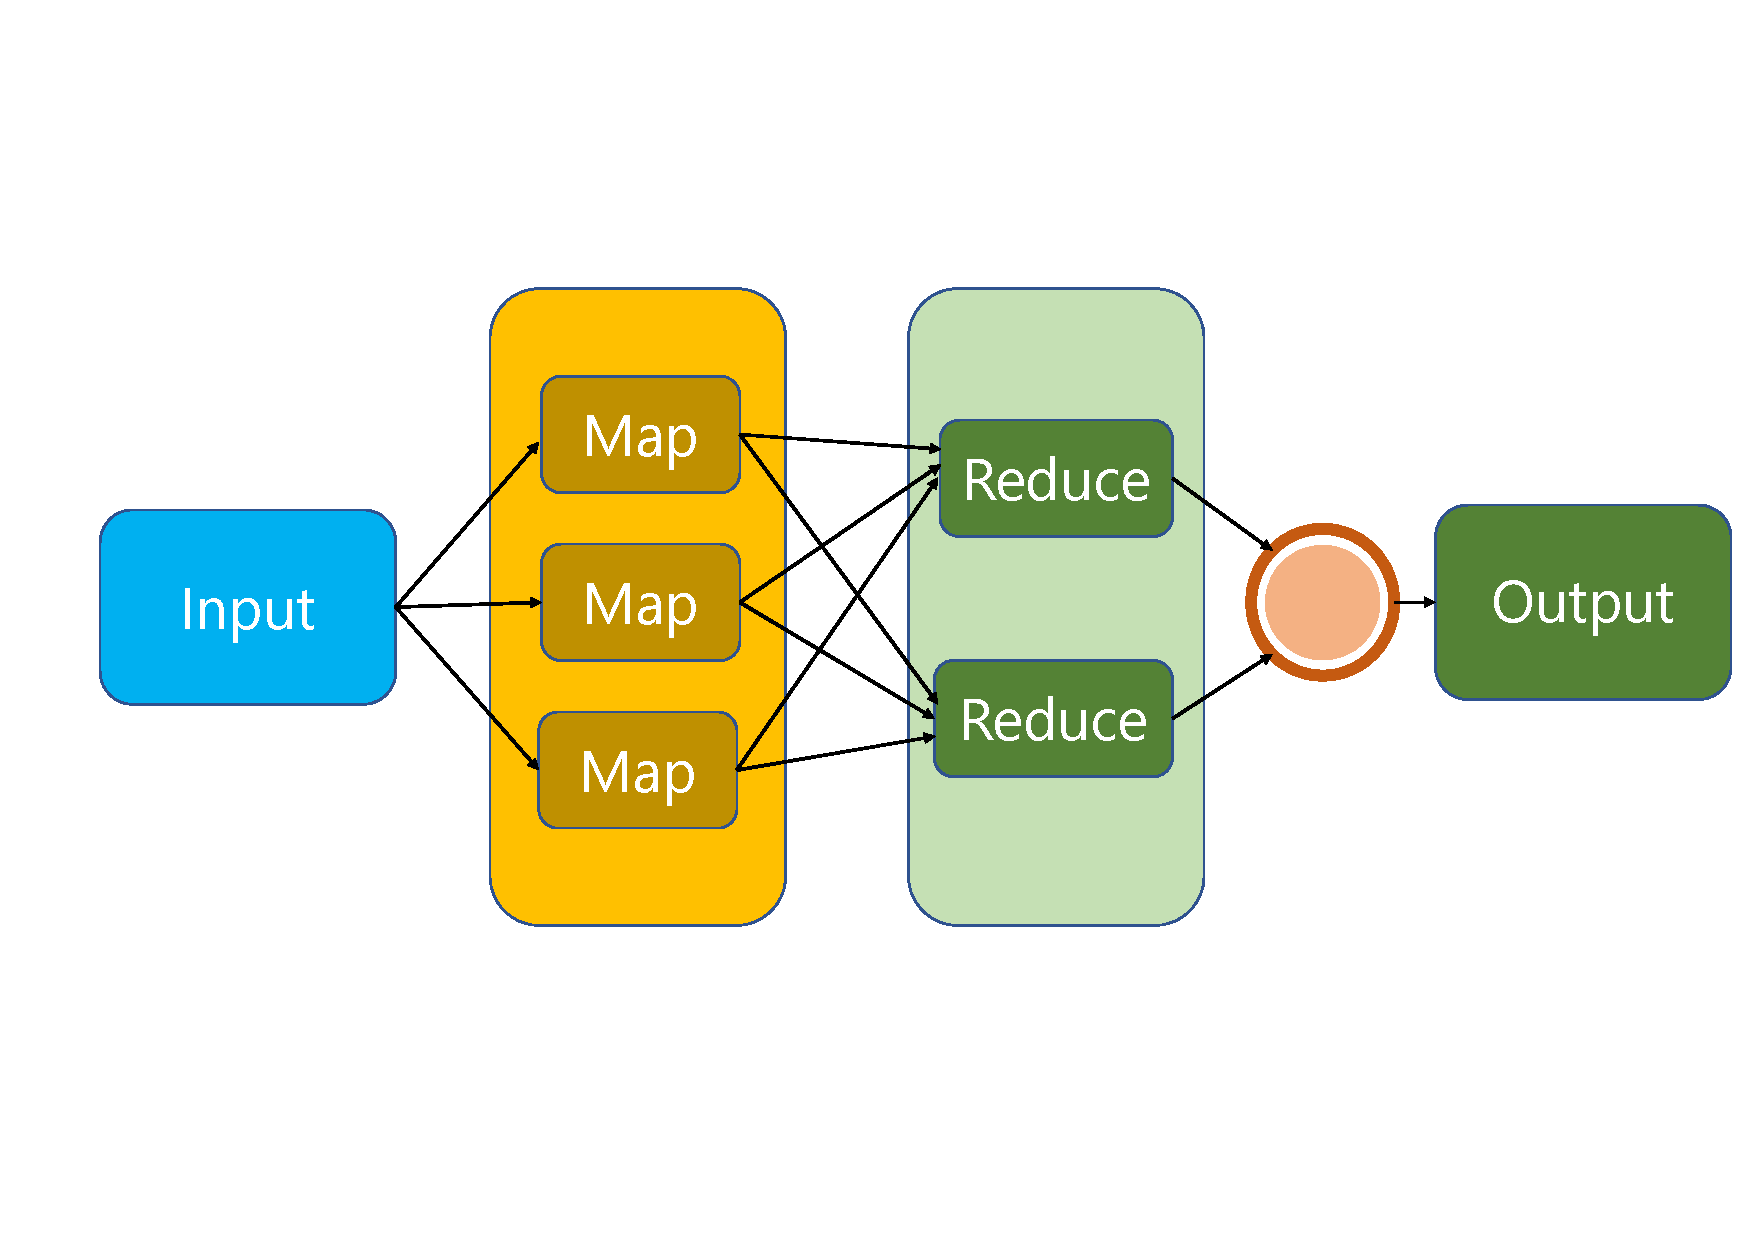
\includegraphics[width=\columnwidth]{Images/map_reduce_1.pdf}  
	\caption[map-reduce model]{Abstract representation of map-reduce paradigm}
	\label{fig:mapReduce}
\end{figure}

MapReduce is a programming framework that allows us to perform distributed and parallel processing on large data sets in a distributed environment.\footnote{Extracted from: https://www.edureka.co/blog/mapreduce-tutorial/}.
\begin{itemize}
	\item MapReduce consists of two distinct tasks – Map and Reduce.
	\item As the name MapReduce suggests, reducer phase takes place after mapper phase has been completed.
	\item So, the first is the map job, where a block of data is read and processed to produce key-value pairs as intermediate outputs.
	\item The output of a Mapper or map job (key-value pairs) is input to the Reducer.
	\item The reducer receives the key-value pair from multiple map jobs.
	\item Then, the reducer aggregates those intermediate data tuples (intermediate key-value pair) into a smaller set of tuples or key-value pairs which is the final output.
\end{itemize}

There are open source implementation of the MapReduce framework, for example Apache Hadoop.
The MapReduce framework is composed by different functions for each step:
\begin{enumerate}
	\item Input Reader
	\item Map Function
	\item Partition Function
	\item Compare Function
	\item Reduce Function
	\item Output Writer
\end{enumerate}

The Input Reader reads the data from mass memory and splits the input in S different splits, with a fixed dimensions (e.g., 64 MB) that are successively distributed to M machines of the cluster that have the Map Function. The Input Reader has also the goal of generating a pair (key, value). The N machine of the cluster are divided in 1 master,
whose goal is to detect idling slaves and assign them a task, and N - 1 slaves that receive the tasks assigned by the master node. In total, M Map tasks and R Reduce tasks are assigned. A slave that has been assigned the M-th task reads the content of the input, extracts the (key, value) pairs and send them to the Map function defined
by the user, that generates zero or more (key, value) pairs as output. These pairs are buffered in memory. Periodically the buffered pairs are cached on disk and partitioned in R sections by the partition function. The addresses of the partitioned sections are sent to the master node which is responsible of rotating the location of the slaves that
will process the Reduce function. Between the slave with the Map function and the one with the Reduce one, all the pairs are reordered in order to find the ones that point at the same value, and thus also have the same key.  
The so called shuffling phase is the process that is used to transfer data from mappers to reducers. Once all the keys that point to the same value have been found using the compare function, a merge operation is performed. The sorting operation is useful because in this way the reducer can know when a new reduce task should start. For each of the keys, the associated slave iterates on all the keys, takes the values with the same key and then applies the Reduce function defined by the user, generating one or more element in output. The Output Writer has the goal of writing the results back to mass storage.
\begin{figure}
	\centering
	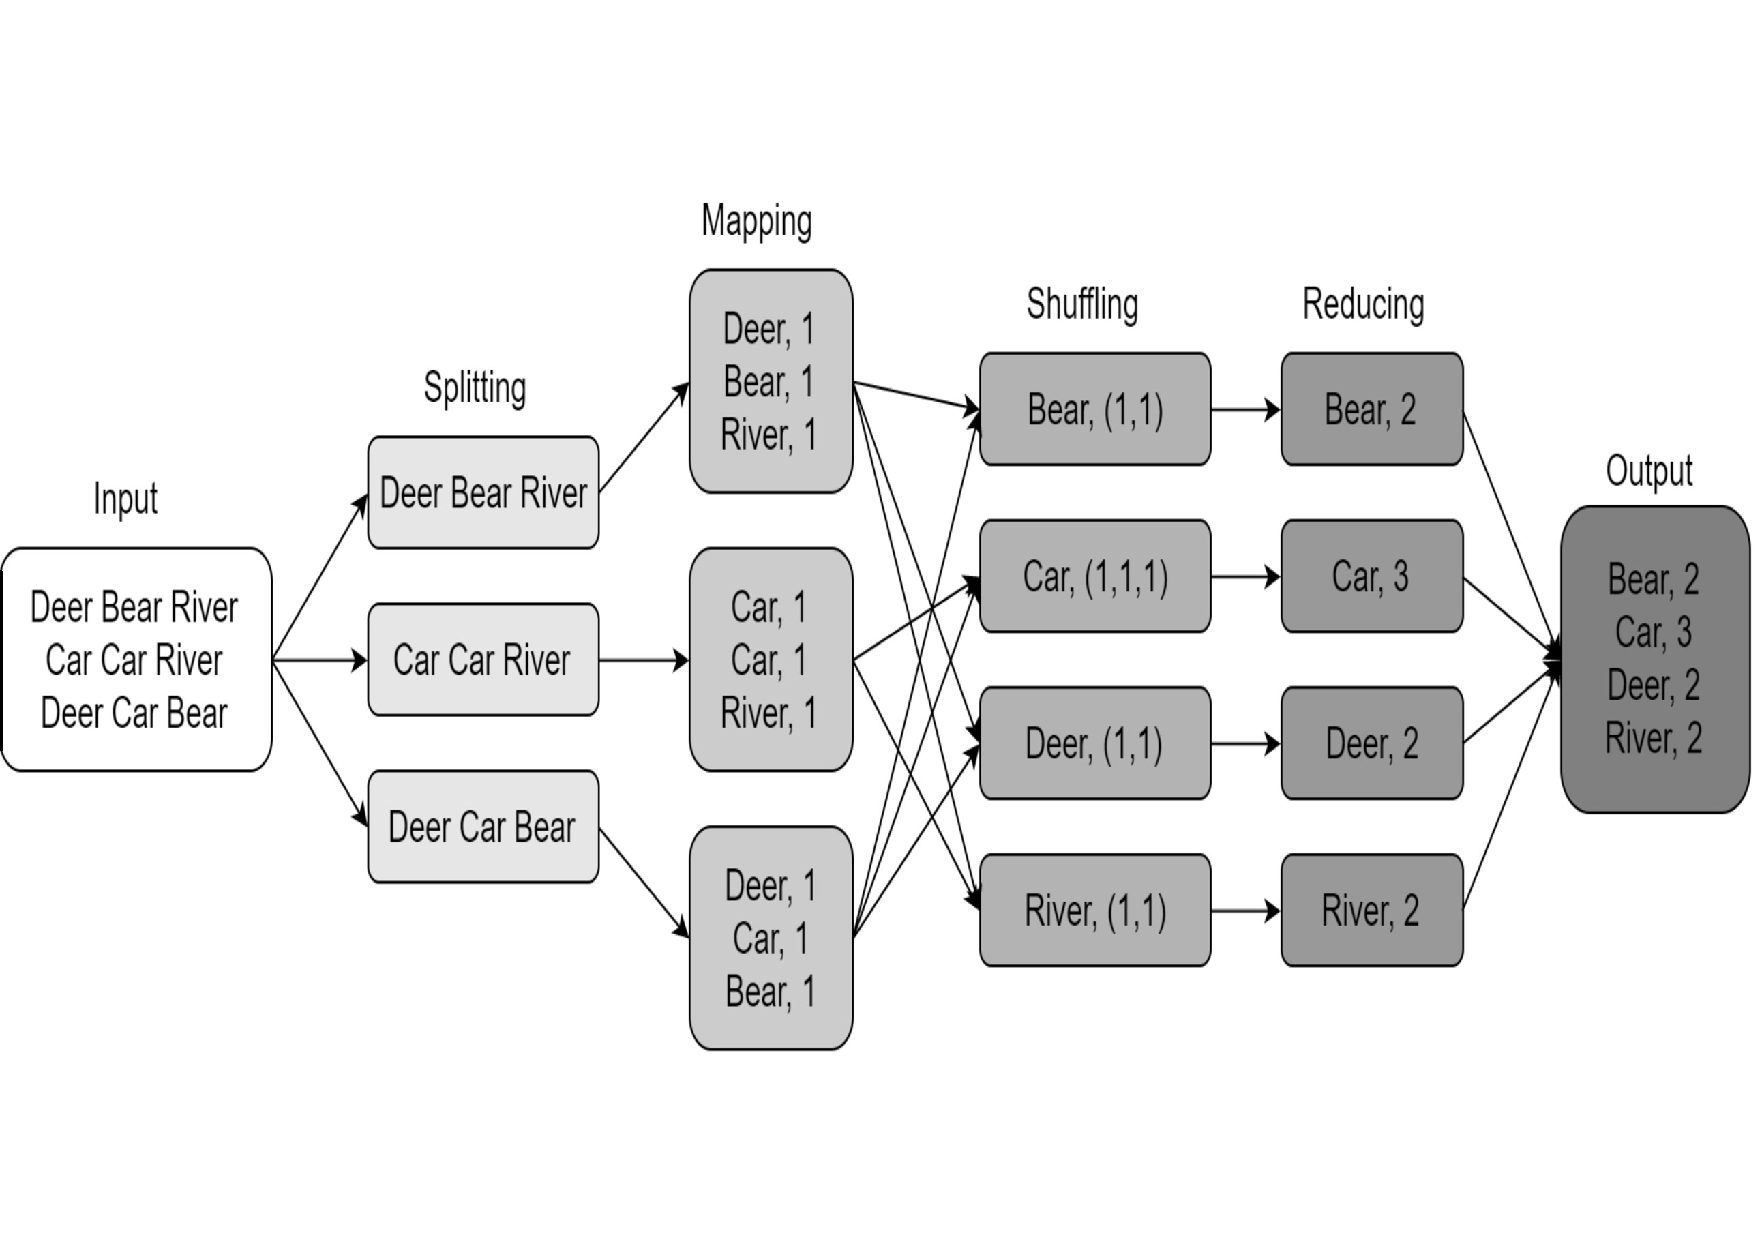
\includegraphics[width=\columnwidth]{Images/word_count_example.pdf}  
	\caption[map-reduce model]{Map-Reduce word count job example. Counts the occurrence of each word in input}
	\label{fig:wordCountExample}
\end{figure}
A sample word count application can be seen in \myFig{fig:wordCountExample} The input is a document containing words, our goal is to compute the number of occurrence of each of the words in the document. Each Map task applies its function on a line of the document, emitting for each of the words in the line a pair (’word’, 1). For example if the input line is "Dear Bear River", it is split into ["Dear", "Bear", "River"] and then mapped into [("Dear", 1), ("Bear", 1), ("River", 1)]. After shuffling the map results, the Reduce task receives a word and a list containing as many ones as the times the word appeared in the document, the reduce function will simply sum the ones in the list, emitting as a
result the pair (’word’, ’count’). For example, a reducer can receive the key "Bear" with list of values (1, 1), this is reduced into ("Bear", 2). Reducers results are then collected and stored in mass storage.

Apache Hadoop\footnote{url: https://hadoop.apache.org/docs/} is an open-source framework for distributed storage and processing of big datasets using MapReduce programming model.

\begin{figure}
	\centering
	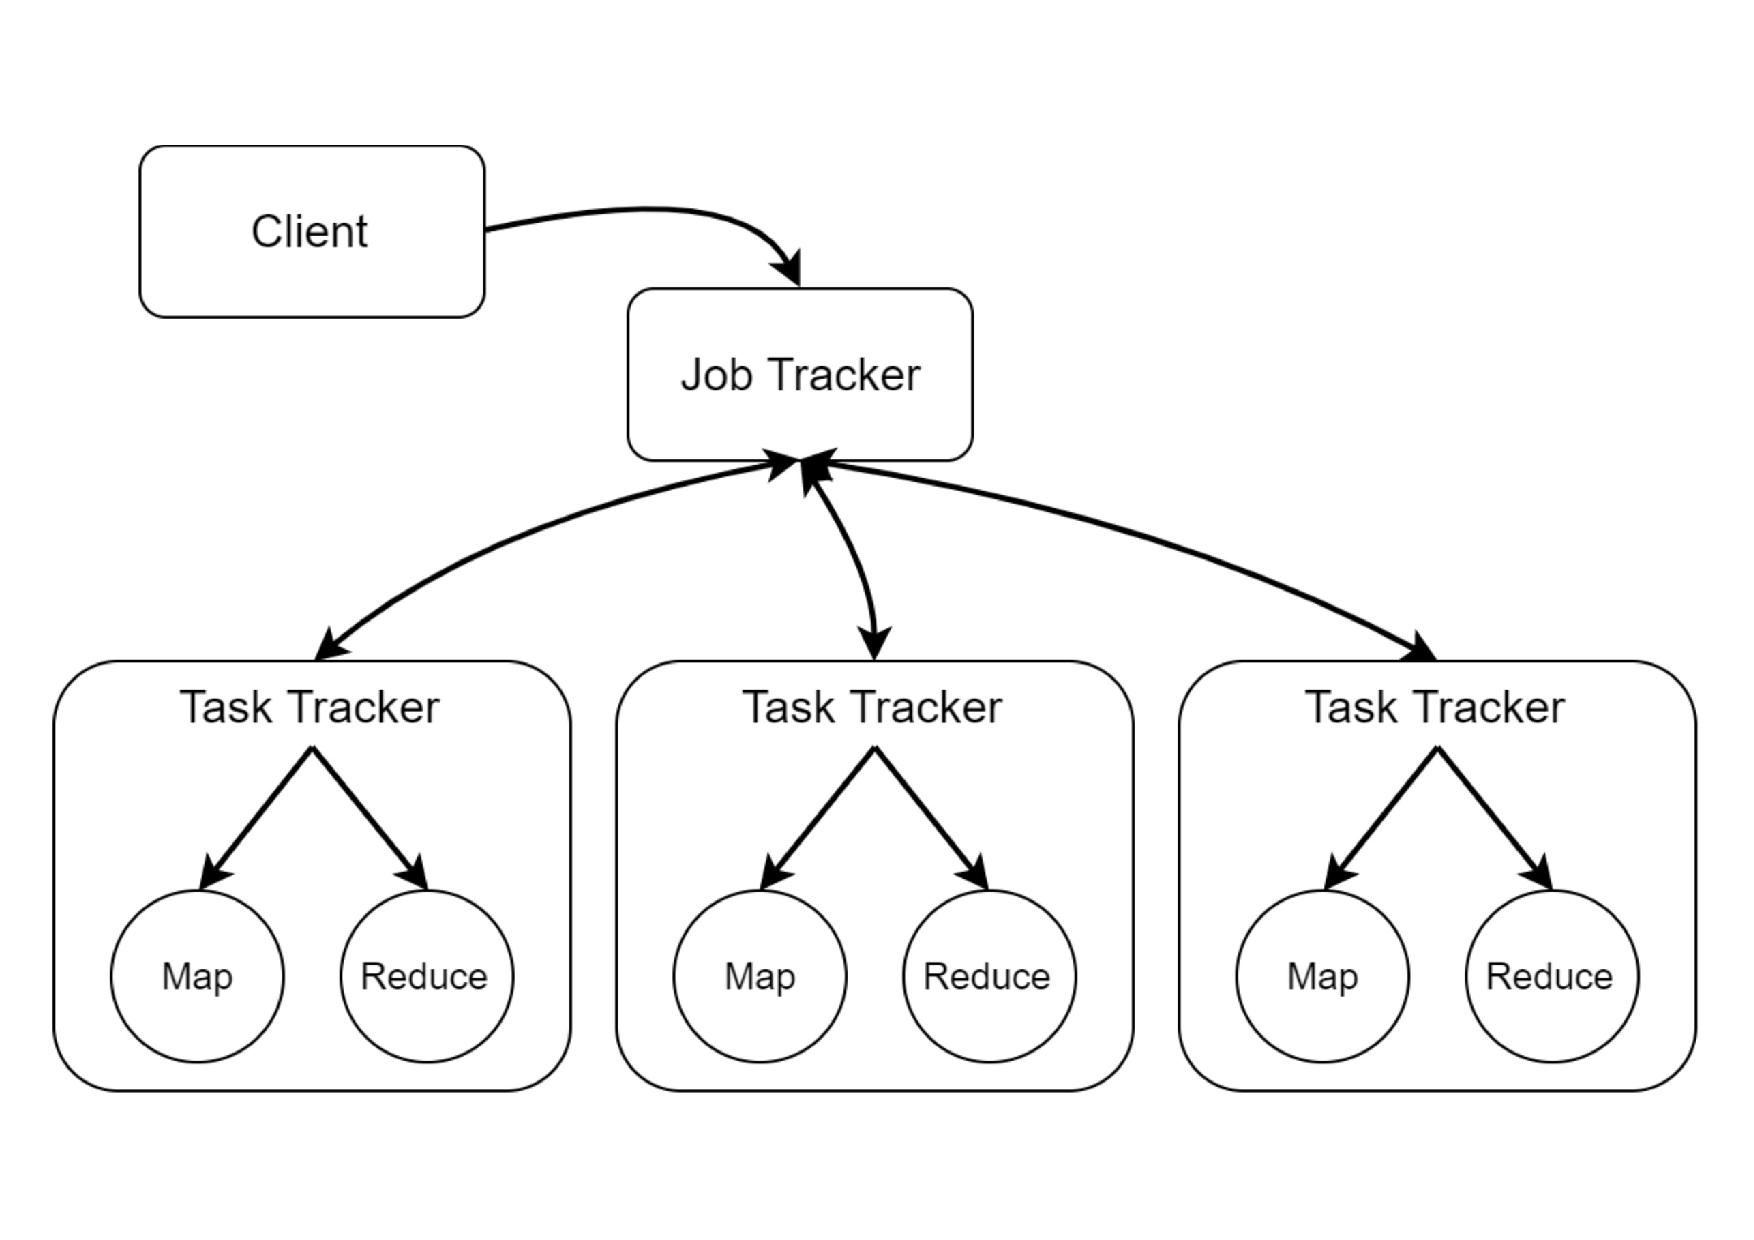
\includegraphics[width=\columnwidth]{Images/hadoop_map_reduce_architecture.pdf}  
	\caption[hadoop map-reduce architecture]{Hadoop Map-Reduce Architecture.}
	\label{fig:hadoopMapReduceArchitecture}
\end{figure}

Apache Hadoop MapReduce cluster have a centralized structure
composed by a single master Job Tracker (JT) and multiple worker nodes running Task Tracker (TT), as shown in  \myFig{fig:hadoopMapReduceArchitecture} JT main goal
is organizing the job tasks on the slave nodes and continuously monitor
the Task Trackers by means of heartbeats. Heartbeats provide a way to retrieve information about the liveliness of the slaves and to
inspect the progress of the executions of the different tasks. In order
to be fault tolerant, if a task execution fails, it is re-executed possibly
on a different slave. JT has the role of the cluster manager, so it
needs also to check the admissibility of the submitted MapReduce
jobs. TT have the objective of running the assigned task. They reply to
heartbeats in order to affirm their liveliness and to update the master
about the progress of the assigned tasks. They are configured with a
fixed number of map and reduce task slots.
As previously introduced, Apache Hadoop also offers a distributed file-system that stores data on different machine, 
providing an high aggregate bandwidth across the cluster. This functionality is called Hadoop Distributed File System (HDFS)\footnote{\textit{HDFS Architecture Guide.} url:  https://hadoop.apache.org/docs/r1.2.1/hdfs\_design.html}. 
It is highly fault tolerant and designed to be deployed on low cost hardware.
\begin{figure}
	\centering
	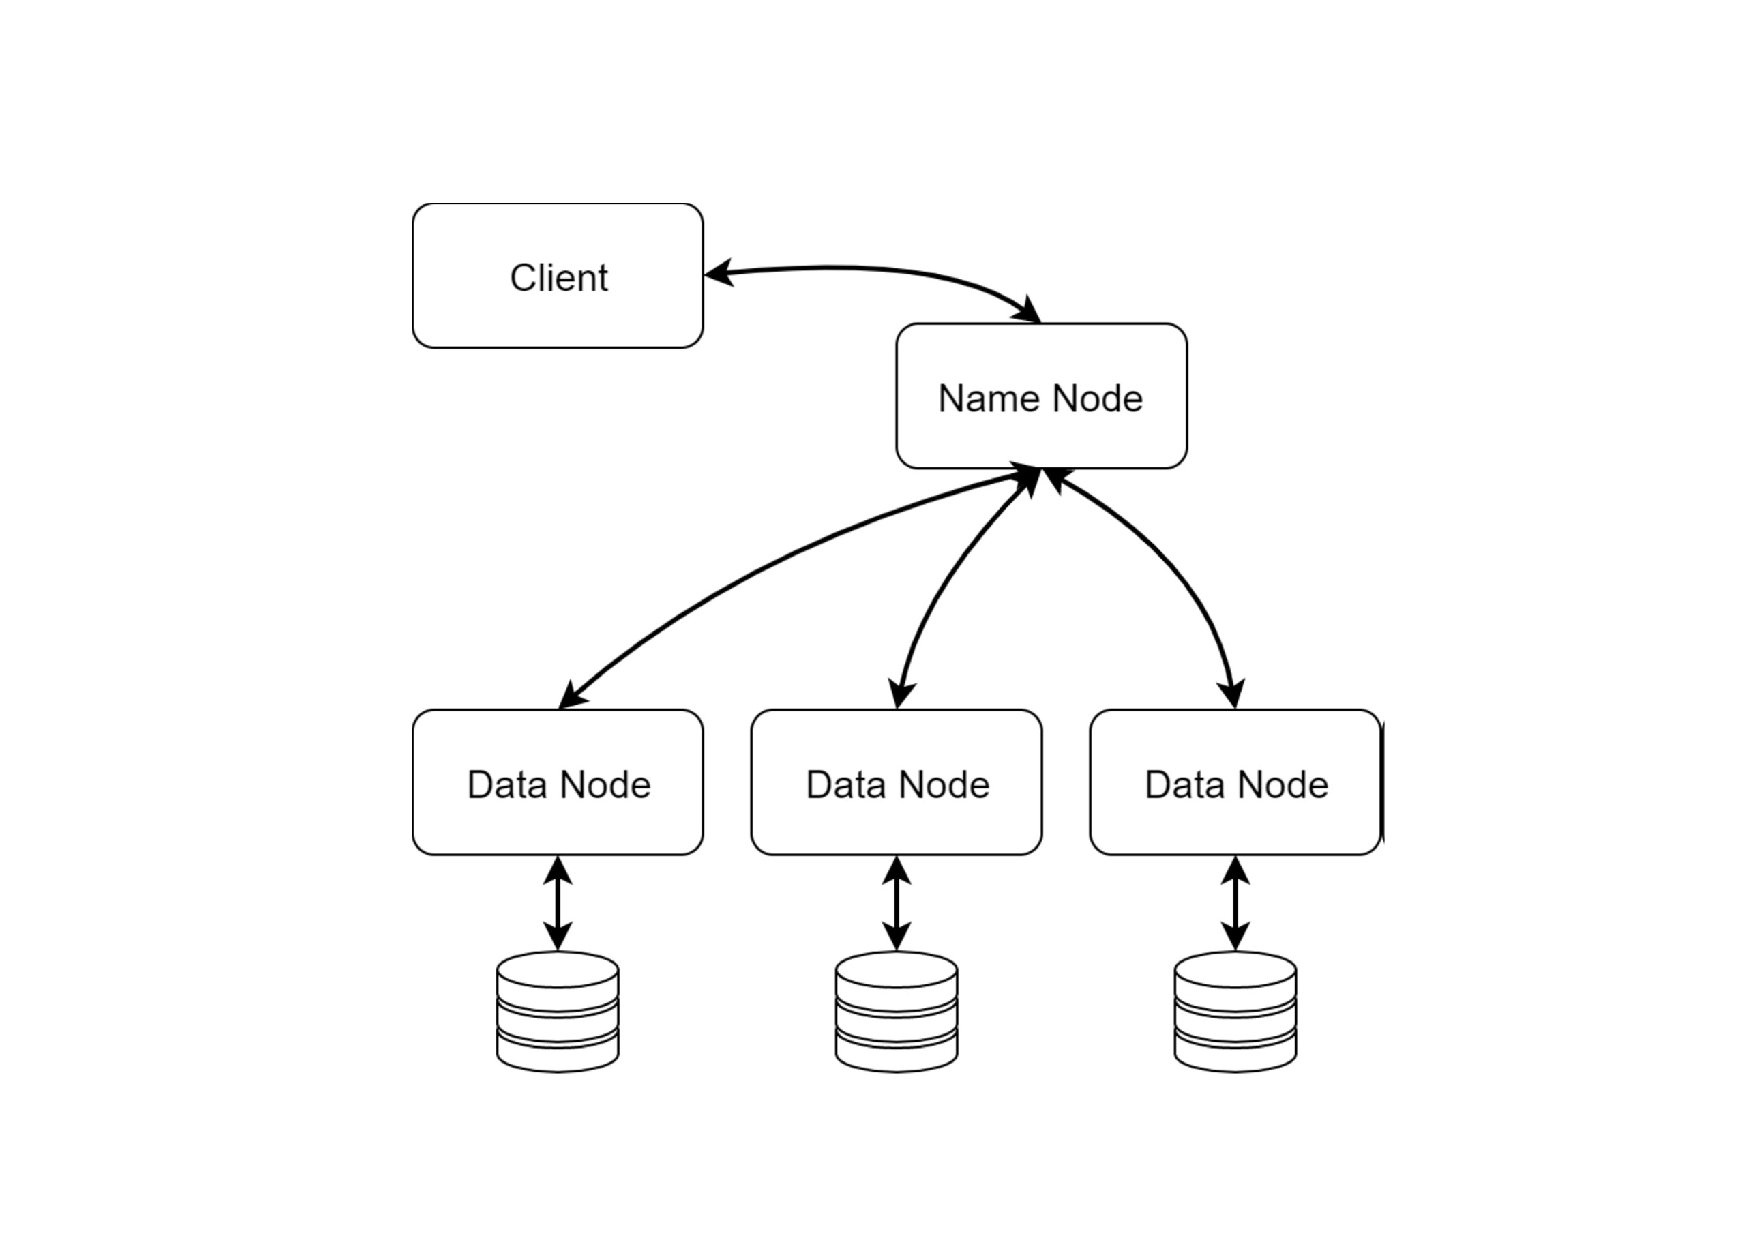
\includegraphics[width=\columnwidth]{Images/hdfs_1.pdf}  
	\caption[HDFS Node Strucure]{HDFS Node Strucure.}
	\label{fig:hdfsNodeStruct}
\end{figure}
HDFS exposes a filesystem namespace and allows user data to be stored in files and
retrieved. Cluster structure is similar to the one of MapReduce cluster,
with one master and multiple slaves, as we can see from \myFig{fig:hdfsNodeStruct}.
The master is composed by a single Name Node (NN), that manages
the file system namespace and regulates access to the files by clients.
NN executes filesystem operations such as opening, closing, renaming
files and directory, but the most important operation performed is
keeping track of the mapping between blocks and Data Node (DN).
Indeed a file stored in HDFS is split into one or more blocks, and those
blocks are stored in the Data Node (DN). Data Node (DN) represent
the slaves, they are usually one per node, and manage the storage that
is attached to the node they are running on. They are responsible for
serving read and write operation requests from the clients, but also
can perform block creation, deletion and replication. Block replication
is a significant way to improve fault tolerance.

\subsection{Batch Processing: Spark}\label{sec:spark}
Apache Spark is an open source framework for distributed computation
~\cite{misc:ApacheSpark}, that provides an interface for programming entire clusters
with implicit data parallelism and fault tolerance. With respect to the MapReduce paradigm, the in-memory multilevel primitives of Spark allow to have performances up to 100 times better in certain applications. Spark can work as standalone or on a cluster manager such as Apache Hadoop Yarn or Apache Mesos. It also needs a distributed storage and can natively use HDFS and other solutions. 

Spark has been designed as a unified engine for distributed data processing. Its programming model resembles the one of MapReduce, but it is extended with a data sharing abstraction called Resilient Distributed Dataset (RDD). Using this abstraction, a wide range of processing workloads can be captured, including SQL, streaming, machine learning and graph processing. The generality of the Spark approach gives great benefits: firsty, applications are easier to develop since there is a unified API,  secondly, it is a lot easier to combine processing tasks. With previous distributed computation framework we needed to write data to mass storage before using them in another engine. Spark, instead, can reuse the same data, often kept in memory.
The programming abstraction at the foundation of Spark is the Resilient Distributed Dataset (RDD), that is a fault-tolerant collection of objects partitioned across the cluster and can be processed in parallel. The users create RDD's by applying operations called "transformations", such as map, filter and group-by, on the data. RDD's can be
backed by a file obtained from an external storage. Spark evaluates RDD's in a lazy mode. This allows the construction of an efficient plan to execute the computation requested by the user. In particular, every transformation operation returns a new RDD, that is the representation of the result of the computation, but the computation is not executed immediately after the transformation request is encountered, but only when a Spark action is met. When an "action" is requested by the user code, Spark checks the entire graph of the transformation and uses it to create an efficient execution plan. For example, if there are many filters and maps in a row, Spark can merge them together and execute as a single operation.
RDDs also offer an explicit support to data sharing among the computations that are ephemeral by default, but can be persisted to disk or memory for rapid reuse. This data sharing is one of the main differences between Spark and the previous computing models
like MapReduce, because all the other operations that Spark can perform are similar to the ones of MapReduce. The data sharing capability allows huge speedups, up to 100 times, in particular when executing interactive queries and iterative algorithms.
RDDs can also recover automatically from a failure. Traditionally, fault tolerance in distributed computing was achieved by means of data replication and checkpointing. Spark instead uses a different approach called lineage. Each RDD keeps track of its transformation graph used to generate the RDD and re-executes the transformation operations on the base data to recover every lost partition. The data recovery based on lineage is significantly more efficient than replication in case of data-intensive workload. In general, recovering lost partitions is faster than re-executing the entire program. Spark was designed to support different external systems for persistent storage, usually it is used in conjunction with a clustered file system like HDFS. Spark is designed as a storage-system-agnostic engine, to make it easy to run computations against data from different sources.
\begin{figure}
	\centering
	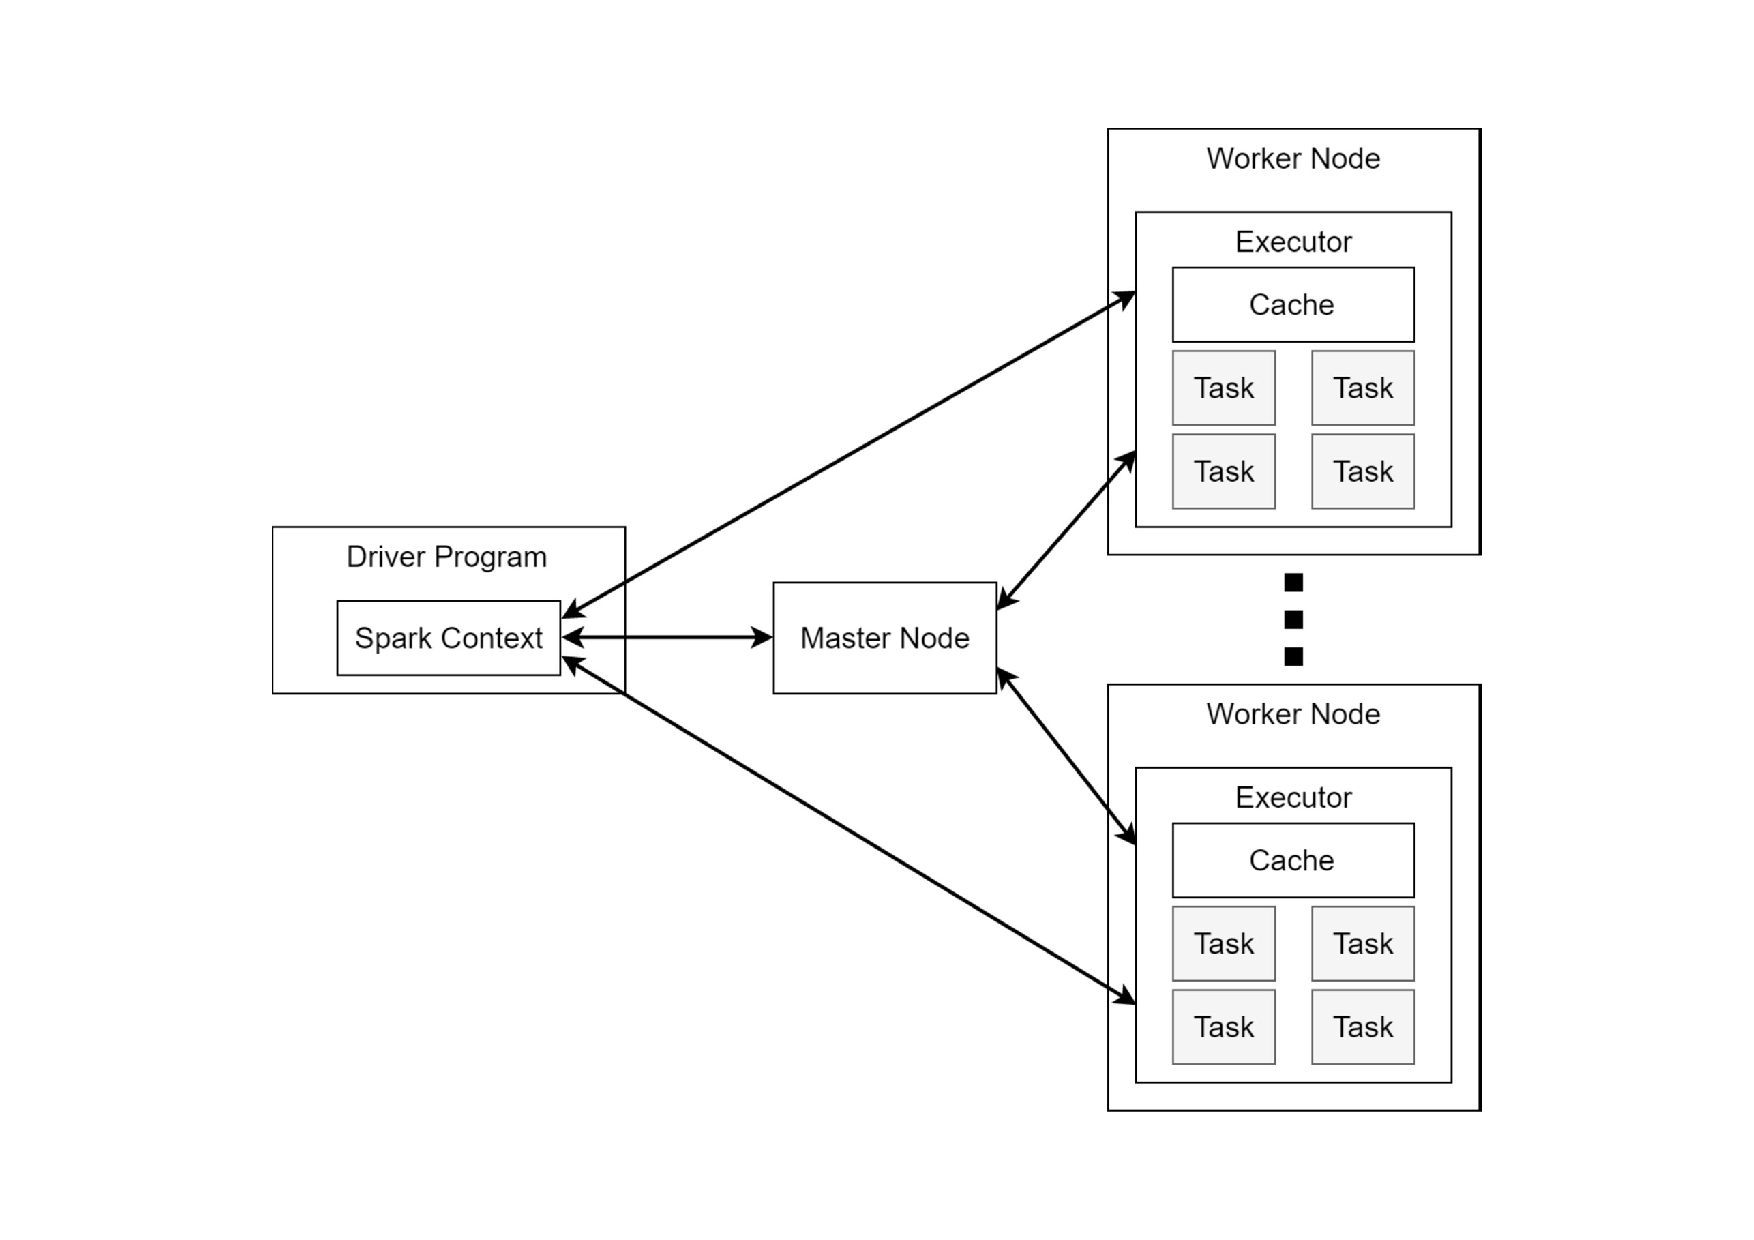
\includegraphics[width=\columnwidth]{Images/spark_standalone_architecture.pdf}  
	\caption[Spark Standalone Architecture]{Spark Standalone Architecture.}
	\label{fig:sparkStandaloneArchitecture}
\end{figure}

Different high-level libraries have been developed in order to simplify
the creation of programs that can run in Spark framework.
\begin{itemize}
	\item SQL and DataFrames: support for relational queries, that are the most common data processing paradigm
	\item Spark Streaming: implements incremental stream processing using a model called "discretized streams", input data is split into micro batches
	\item GraphX: graph computation interface
	\item MLlib: machine learning library, more than 50 common algorithms for distributed model training
\end{itemize}
Spark architecture follows the master/worker paradigm (\myFig{fig:sparkStandaloneArchitecture}). A master server accepts data and processing request, split them into smaller chunk of data and simpler actions that can be handled
in parallel by the multiple workers. A Spark application is executed inside a driver program, that makes the user code executable on the computing cluster using a SparkContext. The driver program is responsible for managing the job flow and scheduling tasks that will run on the executors. The SparkContext will split the requested operations in tasks the can be scheduled for distributed execution on
the workers. When a SparkContext is created, a new Executor process is created on each worker. An executor is a separate Java Virtual Machine (JVM) that runs for the entire lifetime of the Spark application, executes tasks using a thread pool and store data for its Spark application. Communication between the SparkContext and the other
components is performed using a shared bus.
\begin{figure}
	\centering
	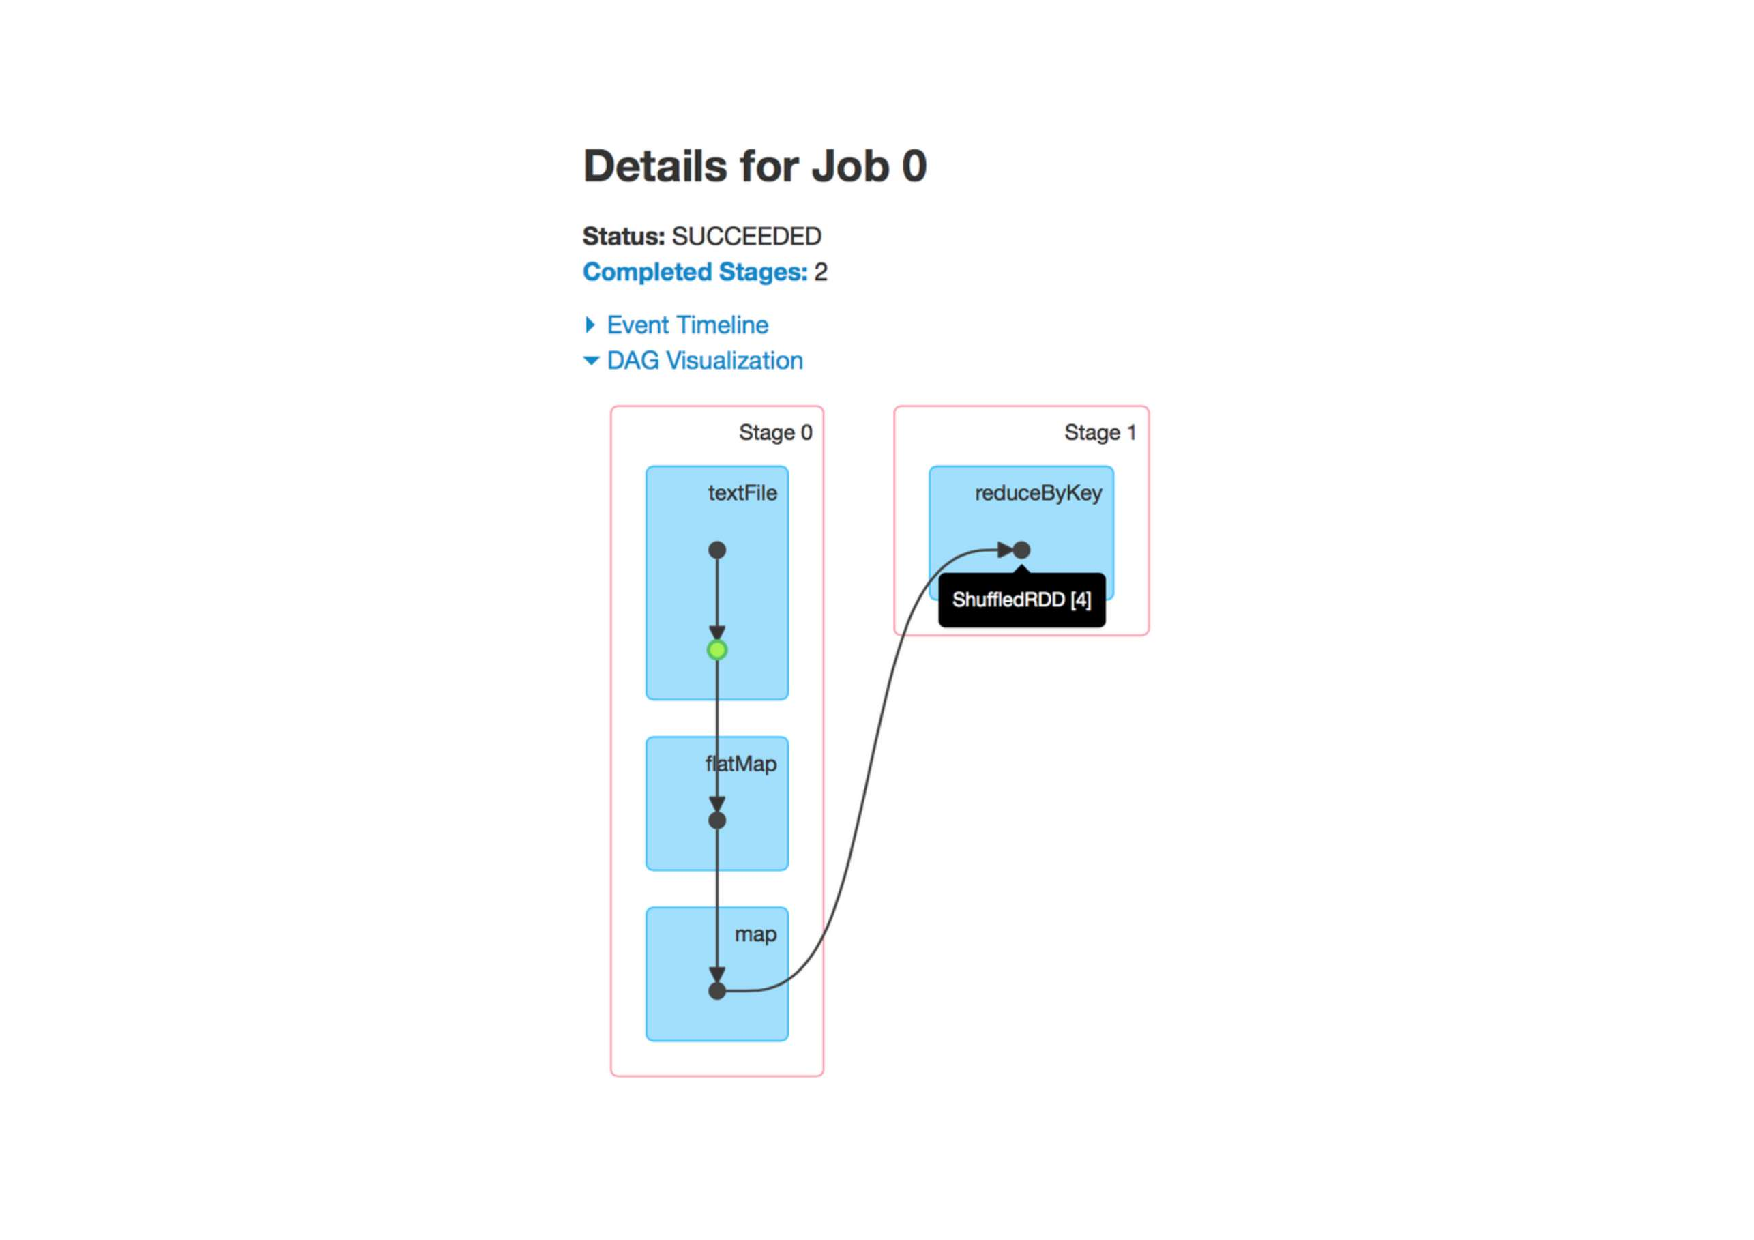
\includegraphics[width=\columnwidth]{Images/spark_dag_example.pdf}  
	\caption[Spark DAG Example]{Spark DAG Example.}
	\label{fig:sparkDAGExample}
\end{figure}
When an application is submitted to Spark, it is divided in multiple jobs. Jobs are delimited by Spark actions in the application code. Spark actions are those operations that return a value to the driver program after running a computation on the dataset.
For each job, a Directed Acyclic Graph (DAG) is created to keep track of the RDDs that are materialized inside the job. DAG nodes represent the RDDs, meanwhile arcs represent transformations, that are the operations that create new datasets from existing ones.
The application steps inside a single job are further organized into stages, that are delimited by operations require data reshuffling, that will inevitably break locality.  Spark distinguishes between narrow transformations, that do not reshuffle data (e.g., map, filter), and wide transformations, that require data reshuffling (e.g., reduceByKey). Stages are also used to produce intermediate result that can be persisted
to memory or mass storage to avoid re-computation. When all stages inside a job
have been identified, Spark can determine which parallel tasks need to be executed for each stage, and schedule them for operation on the executors. Spark creates one task for each partition of the RDD received in input by a stage.

\lstinputlisting[
firstline=1,
lastline=4,
float=tb,
language=Java,
tabsize=2,
numbers=left,
numberstyle=\tiny,
stepnumber=1,
numbersep=5pt,
caption={Spark word count application example.}, 
captionpos=t,
label=lst:wordCount
]{CodeFiles/wordCount.java}

In \MyFig{fig:sparkDAGExample}, we can see a simple DAG representing the single job
of the word count application presented in \MyListing{lst:wordCount} \cite{misc:SparkApplication}. The image was obtained from SparkWeb UI. Through a textFile operation, the input file is read from HDFS. Then a flatMap operation is applied to split each of the lines of the document into words. Following, another
map is used to create (’word’, 1) pairs. Finally, a reduceByKey operation is performed  to count the occurrences of each word. The blue boxes represent the Spark operations that the user calls in his code, while the dots represent the RDDs that are created as a result of these operations. Operations are grouped into stages, represented by the boxes with a red border. The job has been divided into two stages because the reduceByKey transformation requires the data to be shuffled. The green dot represents a cached RDD, in particular the data read from HDFS has been cached, in this way future computations on this RDD can be done faster since data will be read from memory instead of HDFS. The default deployment of Spark is in standalone mode, that is using its embedded cluster manager. 

\subsection{Streams Processing: Flink}\label{sec:flink}
\begin{figure}
	\centering
	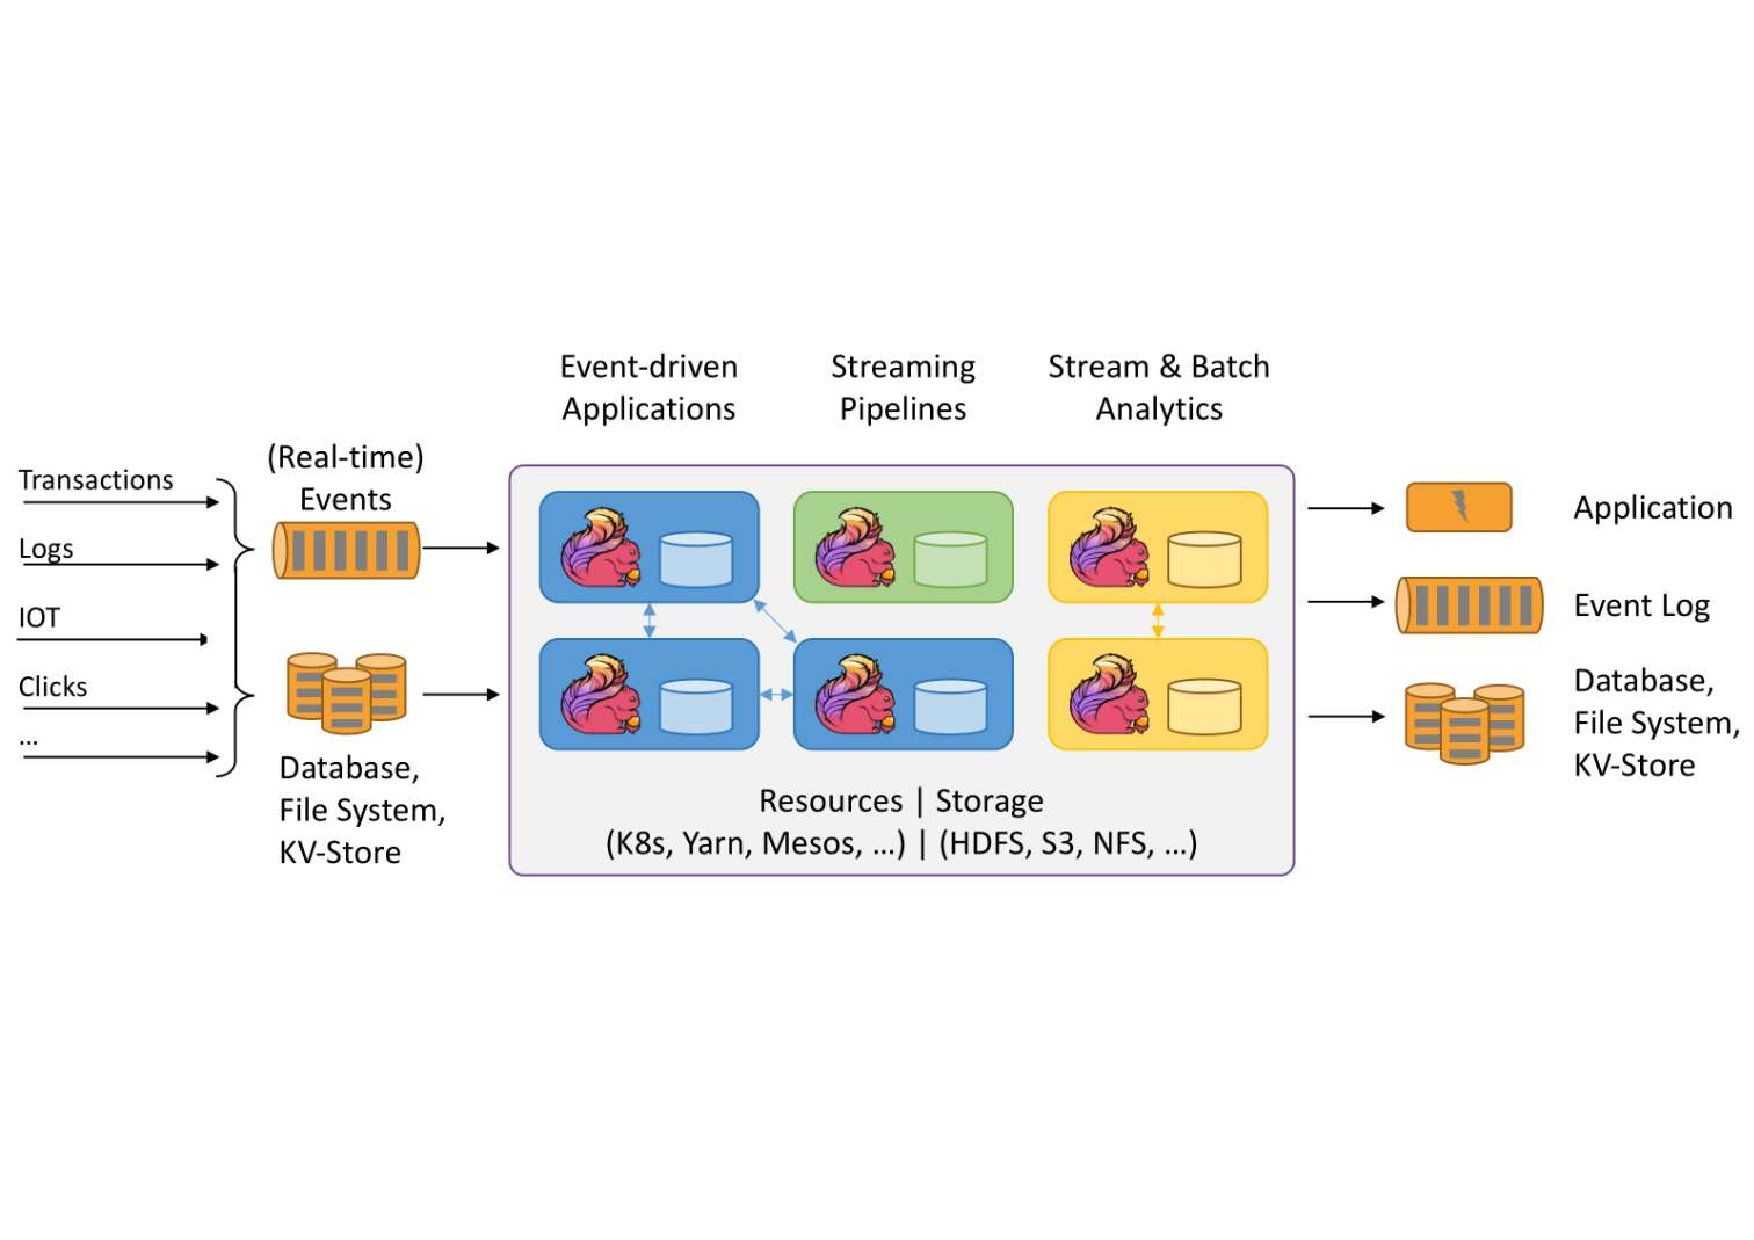
\includegraphics[width=\columnwidth]{Images/apache_flink.pdf}
	\caption[Apache Flink® - Stateful Computations over Data Streams.]{Apache Flink® - Stateful Computations over Data Streams.}
	\label{fig:apache_flink}
\end{figure}
\begin{figure}
	\centering
	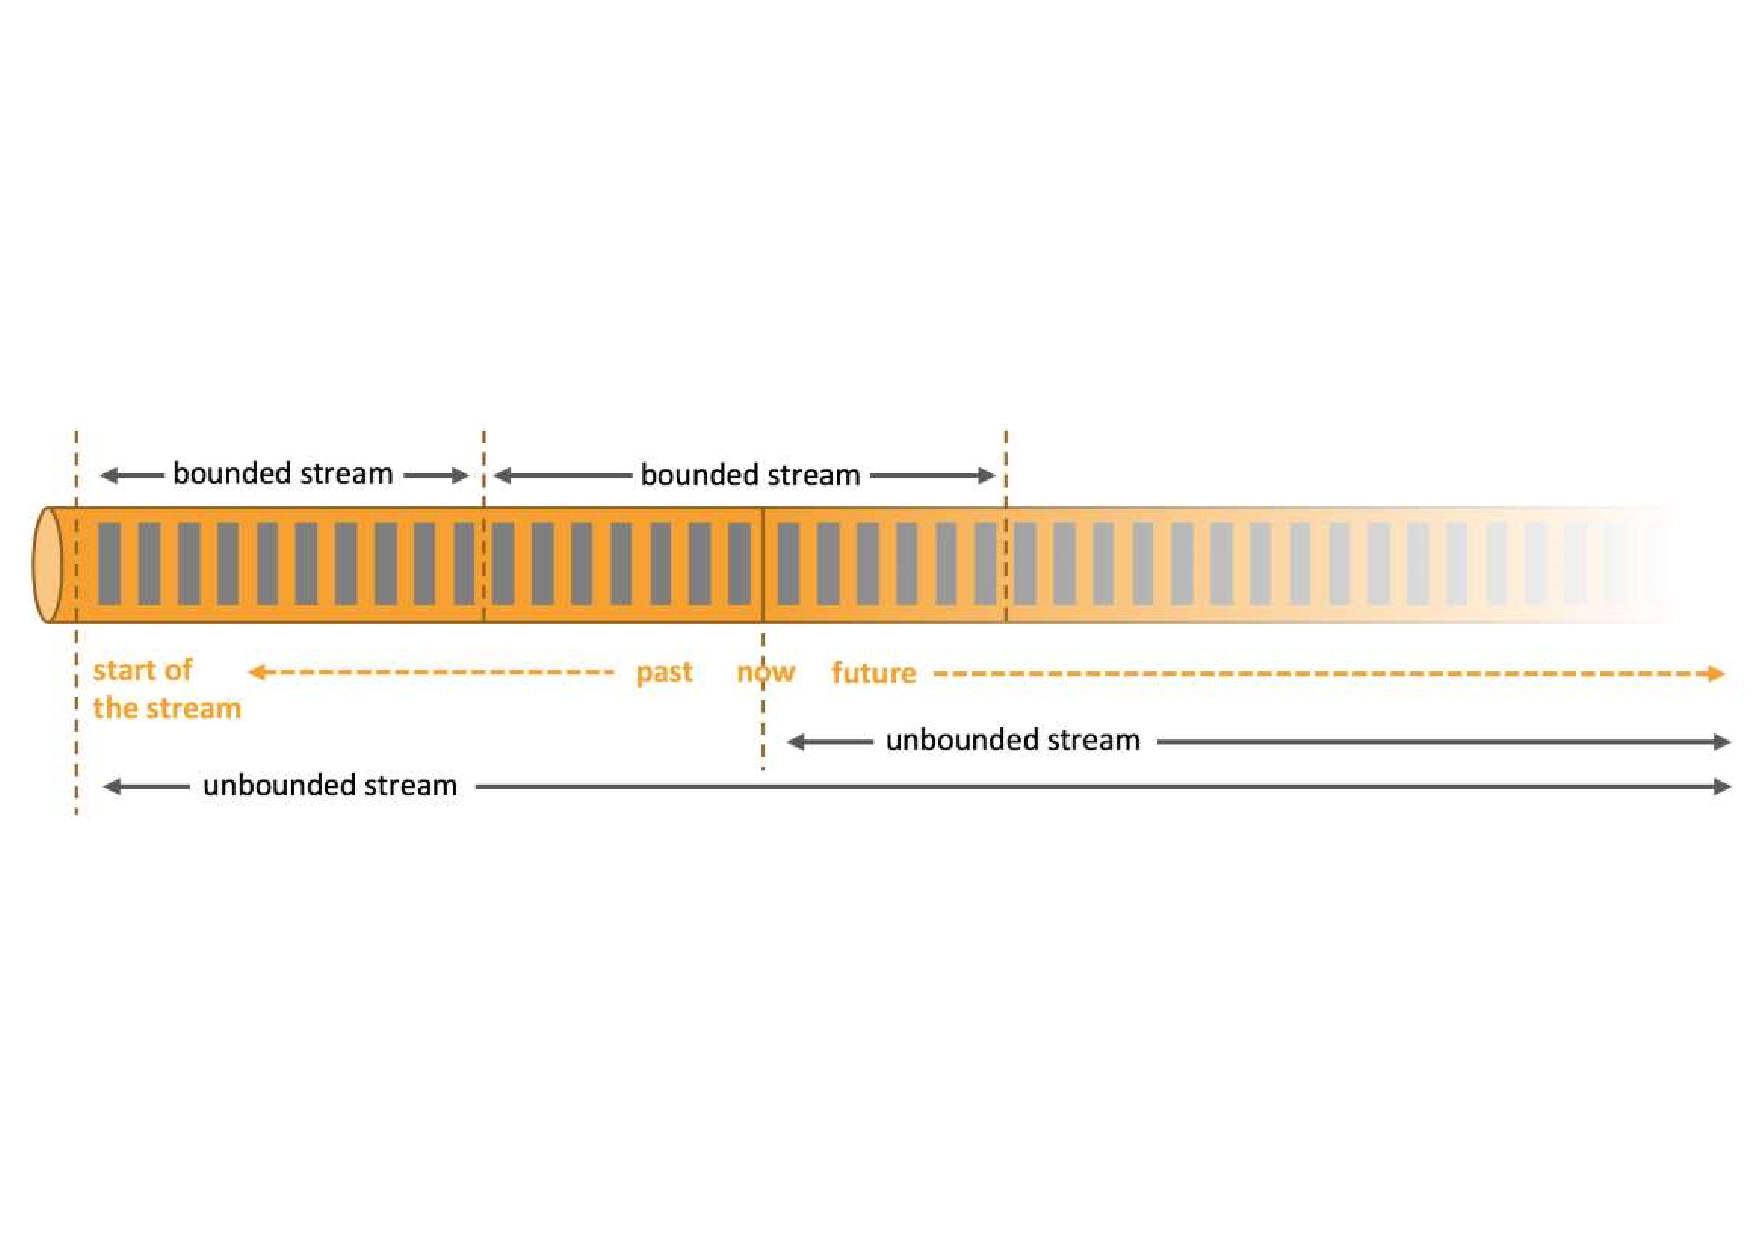
\includegraphics[width=\columnwidth]{Images/apache_flink_data_streams.pdf}
	\caption[Apache Flink® - Bounded \& Unbounded Data Streams.]{Apache Flink® - Bounded \& Unbounded Data Streams.}
	\label{fig:apache_flink_data_streams}
\end{figure}

Apache Flink~\cite{misc:ApacheFlink} is a framework and distributed processing engine for stateful computations over unbounded and bounded data streams. It can run in any commonly used cluster environments, computes at in-memory speed and manages data at any scale.

Flink’s architecture is suitable for processing unbounded and bounded data. Any type of data is generated as a stream of events. Sensors data, server logs or user interactions on a website or mobile application, credit card transactions, all of these data are generated as streams of data.

Data can be processed as unbounded or bounded streams~\cite{misc:ApacheFlinkArchitecture}. 

Unbounded streams have a start but no defined end. They do not terminate and provide data as it is generated. Unbounded streams must be continuously processed, i.e., events must be promptly handled after they have been ingested. It is not possible to wait for all input data to arrive because the input is unbounded and will not be complete at any point in time. Processing unbounded data often requires that events are ingested in a specific order, such as the order in which events occurred, to be able to reason about result completeness.

Bounded streams have a defined start and end. Bounded streams can be processed by ingesting all data before performing any computations. Ordered ingestion is not required to process bounded streams because a bounded data set can always be sorted. Processing of bounded streams is also known as batch processing.


Apache Flink excels at processing unbounded and bounded data sets. Precise control of time and state enable Flink’s runtime to run any kind of application on unbounded streams. Bounded streams are internally processed by algorithms and data structures that are specifically designed for fixed sized data sets, yielding excellent performance.

\subsection{Streams Processing: Storm}\label{sec:storm}

\begin{figure}
	\centering
	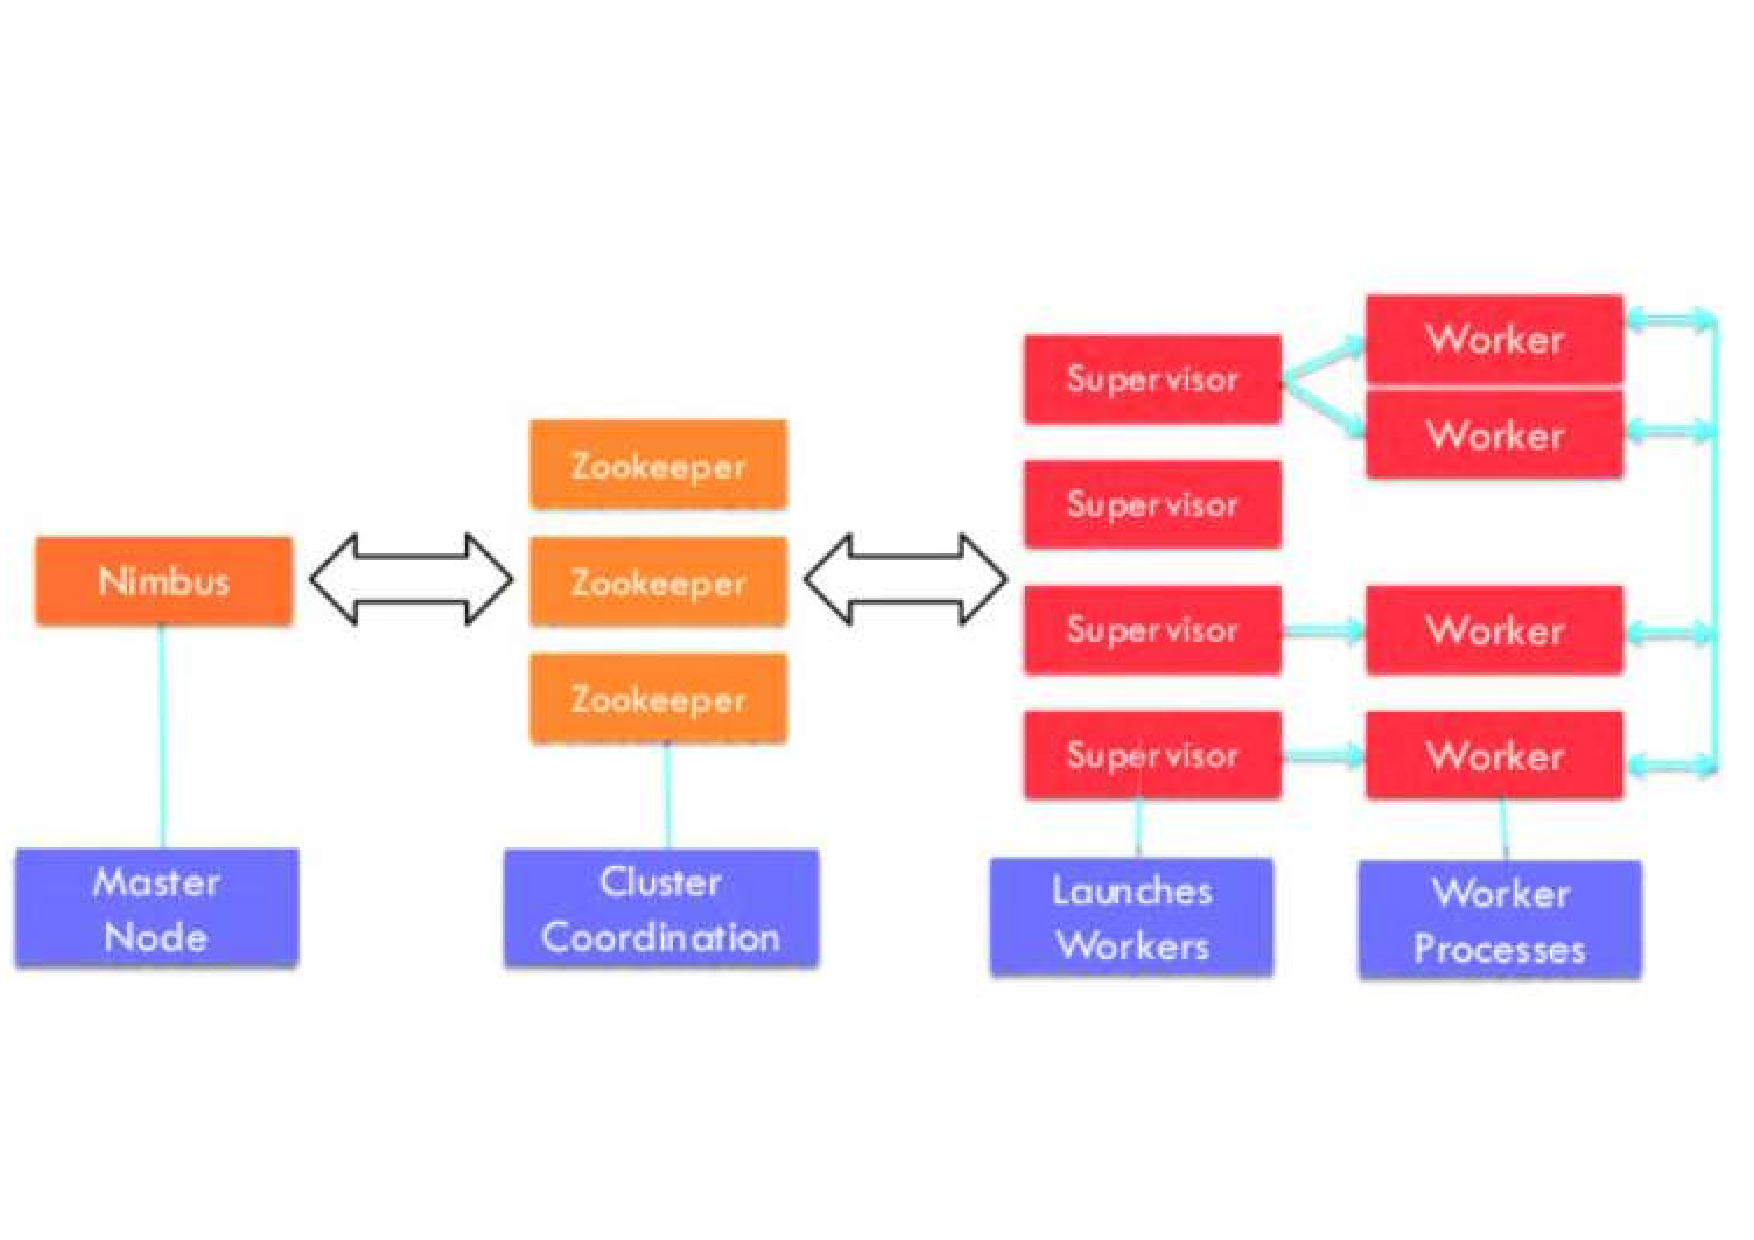
\includegraphics[width=\columnwidth]{Images/apache_storm.pdf}
	\caption[Apache Storm.]{Apache Storm.}
	\label{fig:apache_storm}
\end{figure}
\begin{figure}
	\centering
	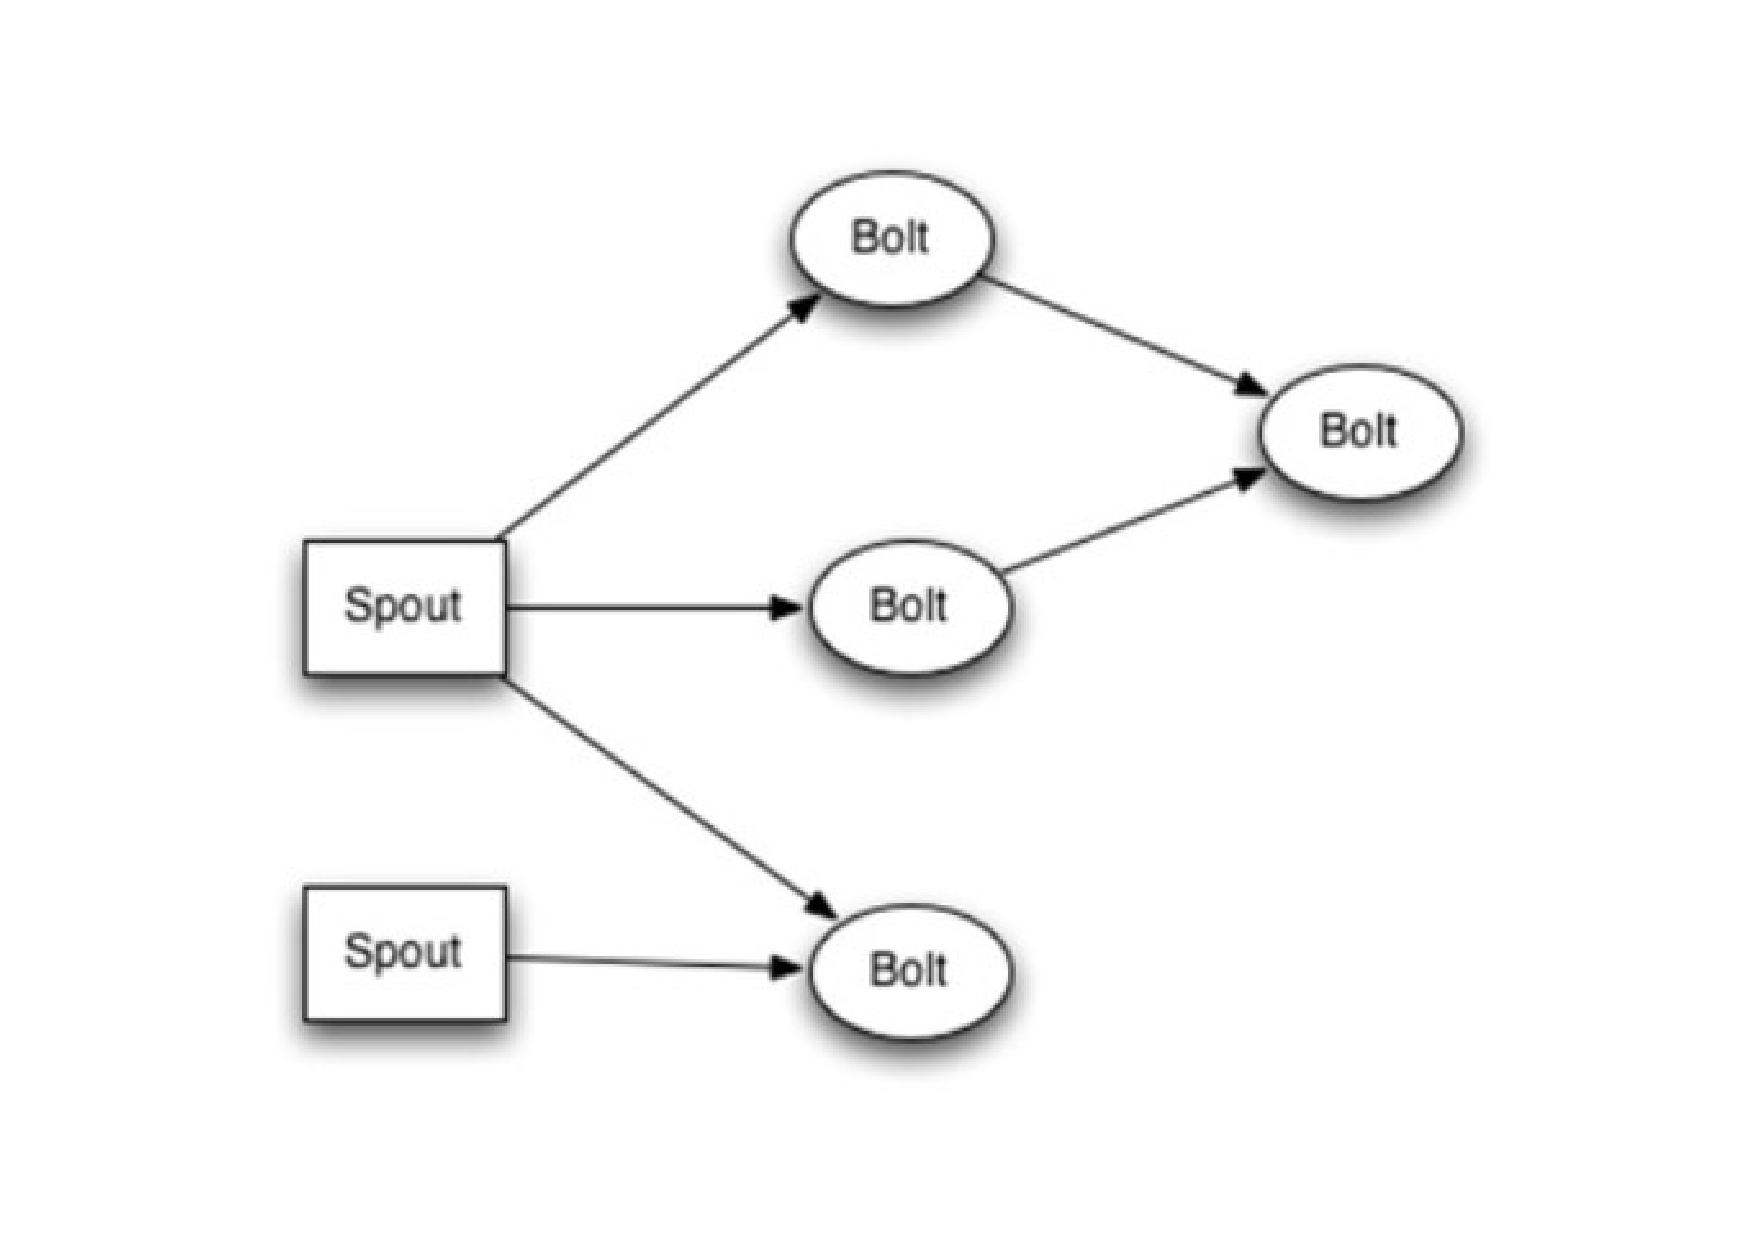
\includegraphics[width=\columnwidth]{Images/apache_storm_components_abstraction.pdf}
	\caption[Apache Storm Components Abstraction.]{Apache Storm Components Abstraction.}
	\label{fig:apache_storm_components_abstraction}
\end{figure}

Apache Storm~\cite{misc:ApacheStorm} is a free and open source distributed realtime computation system. Storm makes it easy to reliably process unbounded streams of data, doing for realtime processing what Hadoop did for batch processing. Storm is simple, can be used with any programming language, and is easy to use.

Storm has many use cases: realtime analytics, online machine learning, continuous computation, distributed RPC, ETL, and more. Storm is fast: a benchmark clocked it at over a million tuples processed per second per node. It is scalable, fault-tolerant, guarantees your data will be processed, and is easy to set up and operate.

Storm integrates with the queueing and database technologies you already use. A Storm topology consumes streams of data and processes those streams in arbitrarily complex ways, repartitioning the streams between each stage of the computation however needed. 

The Apache Storm architecture is quite similar to that of Hadoop. However there are certain differences which can be better understood by getting a closer look at its cluster in \MyFig{fig:apache_storm}: 
\textbf{Nodes} - There are two types of nodes in Storm cluster similar to Hadoop:
\begin{itemize}
	\item {Master node - }The master node of Storm runs a daemon called ‘Nimbus’, which is similar to the ‘Job Tracker’ of Hadoop cluster. Nimbus is responsible for distributing codes, assigning tasks to machines and monitoring their performance.
	\item {Worker node – }Similar to the master node, the worker node also runs a daemon called ‘Supervisor’ which is able to run one or more worker processes on its node. Each supervisor works assigned by Nimbus and starts and stops the worker processes when required. Every worker process runs a specific set of topology which consists of worker processes working around machines. Since Apache Storm does not have the abilities to manage its cluster state, it depends on \textbf{Apache Zookeeper} for this purpose. Zookeeper facilitates communication between Nimbus and Supervisors with the help of message acknowledgements, processing status, etc.
\end{itemize}
\textbf{Storm Components/Abstractions} (see  \MyFig{fig:apache_storm_components_abstraction}) – There are basically four components which are responsible for performing the tasks:

\begin{itemize}
	\item Topology – Storm Topology can be described as a network made of \textbf{spouts} and \textbf{bolts}. It can be compared to the Map and Reduce jobs of Hadoop. Spouts are the data stream source tasks and Bolts are the accrual processing tasks. Every node in the network consists of processing logic’s and links to demonstrate the ways in which data will pass and the processes will be executed. Each time a topology is submitted to the storm cluster, Nimbus consults the supervisor nodes about the worker nodes. 
	\item Stream – One of the basic abstractions of the storm architecture is stream which is an unbounded pipeline of tuples. A tuple can be defined as the fundamental component in the Storm cluster containing a named list of the values or elements.  \item Spout – It is the entry point or the source of streams in the topology. It is responsible for getting in touch with the actual data source, receiving data continuously, transforming those data into actual stream of tuples and finally sending them to the bolts to be processed. two types of nodes in Storm cluster.
	\item Bolt - Bolts keep the logic required for processing. These are responsible for emitting the streams for processing by other bolts and saving or sending the data for storage. These are capable of running functions, filtering tuples, aggregating and joining streams, linking with database, etc.
\end{itemize}

\section{Runtime Management of Big Data Applications}\label{sec:runtime_mgmt_big_data_apps}
Big data applications requires system scalability, fault tolerance and  availability~\cite{articleBigData:2017}. 

\textit{Scalability} means the ability to maintain an approximate linear relationship between the size of processed data and the amount of consumed resources. 

\textit{Fault tolerance} is a challenge, especially when systems are complex and involve many networked nodes. By means of hardware virtualization, cloud computing services satisfies all the requested requisites, and the \textit{elasticity} and redundancy it provides  also enable big data application high availability, scalability and fault tolerance.

Another very important feature of big data applications is the \textit{Quality of Service} or \qos.

\qos definition for IT applications differ by application type. Interactive applications are usually assessed according to response time or throughput, and their fulfillment depends on the intensity and variety of the incoming requests. 

Big data applications might require a single batch computation on a very large dataset, thus \qos must consider the execution of a single run. In this domain \qos is often called \textit{deadline}, or the desired duration of the computation. 

We have mentioned availability, fault tolerance and availability as fundamental requirements and \qos as a measure of the capability to meet a user-defined deadline when processing big data. Many factors influence the duration of an application execution, surely resource allocation greatly influences the duration. 

The challenges introduced by big data require resilient, flexible and self-adapting software systems~\cite{DeLemos2013}. Hence, \textit{autonomic system}s and \textit{self-adaptation} has increasingly captured the attention of researchers ~\cite{Weyns:2012:CSE:2666795.2666811}. These systems automatically react to changes in the environment, or in their own state, and change their behaviour to satisfy functional and non-functional requirements. Meeting requirements in complex and variable execution environments is a difficult task that can be tackled at design time or at runtime. At runtime the adaptation is very often obtained by using a well-known process called MAPE~\cite{MAPE}, a control loop composed of four phases: monitoring, analysis, planning and execution.

One of the challenges that modern software systems face is the provisioning and optimization of resources to meet a varying demand, generated by are increasingly common phenomena like fluctuating workloads, unpredictable peaks of traffic and unexpected changes. Service providers cannot disregards these factors if they want to cope with the challenge of satisfying functional and non-functional requirements, usually defined in SLAs (Service Level Agreements). Hence the need arises for an automatic adjustment of system resources allocation to avoid resource saturation and unresponsiveness, users dissatisfaction and unnecessary costs. This paradigm is called elastic resource provisioning~\cite{Dustdar2011, Zhang2010, Sehgal2012, Herbst2013}.

Many approaches about elastic systems and dynamic resource allocation were proposed both in the industry and in academia. In modern technology elasticity is often enabled by cloud computing that gives to an application a theoretical infinite degree of scalability. However considering only resources is rather restrictive because of the many factors that impact application during their runtime life-cycle. In fact Dustdar et al.~\cite{Dustdar2011} argue that elastic computing should be designed by considering three dimensions: quality, resources and cost.  Quality elasticity considers how quality is affected by a change in resource availability. Instead cost elasticity measures how resource provision is affected when a change in cost happens. 

Cloud computing services provide the needed level of fault tolerance and availability required by big data applications. In the remainder of this chapter we present an overview of popular big data frameworks that can leverage cloud computing solutions and how they address elastic resource allocation to satisfy functional and non-functional application requirements. The resulting scenario represent the base for our work, where we will consider quality elasticity and not cost elasticity aspect. 

This thesis shows how the application of lightweight symbolic execution tecniques to deadline-based \qos constrained multi-DAG big data applications helps reduce the number of deadline violations and allocate resources more efficiently.


\section{Elastic Resource Provisioning}
\label{Section:Introduction:ElasticProvisioning}

The word \textit{elasticity} comes from physics and is defined as the ability of an object or material to resume its normal shape after being stretched or compressed. In computing, elasticity has a similar meaning and is used to characterize \textit{autonomic systems}. Herbst et al.~\cite{Herbst2013} defines elastic provisioning as reported below.
\begin{quote}
	\textit{\textbf{Elasticity} is the capability of a system to adapt to workload changes by provisioning or de-provisioning resources automatically such that at each point in time the available resources match the current demand as closely as possible}.
\end{quote}

A system is in an \textit{under provisioned} state if it allocates less resources than required by the current demand; it is in an \textit{over provisioned} state if allocates more resources than required. Moreover, elasticity is determined by four attributes:

\begin{itemize}
	\item \textit{Autonomic Scaling}: the adaptation process used to control the system.
	\item \textit{Elasticity Dimensions}: the set of scaled resources in the adaptation process.
	\item \textit{Resource Scaling Units}: the minimum amount of allocable resources to each dimension.
	\item \textit{Scalability Bounds}: the lower and the upper bound on the amount of resources that can be allocated to each dimension.
\end{itemize}

Additionally, two aspects must be considered in evaluating the elasticity degree of a system: speed and precision. 

\textbf{Speed of scaling up/down:} the time it takes to switch from an underprovisioned/overprovisioned state to an optimal or overprovisioned/underprovisioned state respectively. 

\textbf{Precision of scaling}: the absolute deviation of the current amount of allocated resources from the actual resource demand.

Scalability and efficiency are terms related to elasticity, nevertheless they differ by the following aspects:
 
\textbf{Scalability}, although is a prerequisite for elasticity, it does not consider the temporal aspects (how fast and how often) and the granularity of the adaptation actions.

\textbf{Efficiency}, contrary to elasticity, it takes in account all the types of resources employed to accomplish a certain amount of work, not only the resources scaled by the adaptation actions. 

\begin{figure}
	\centering
	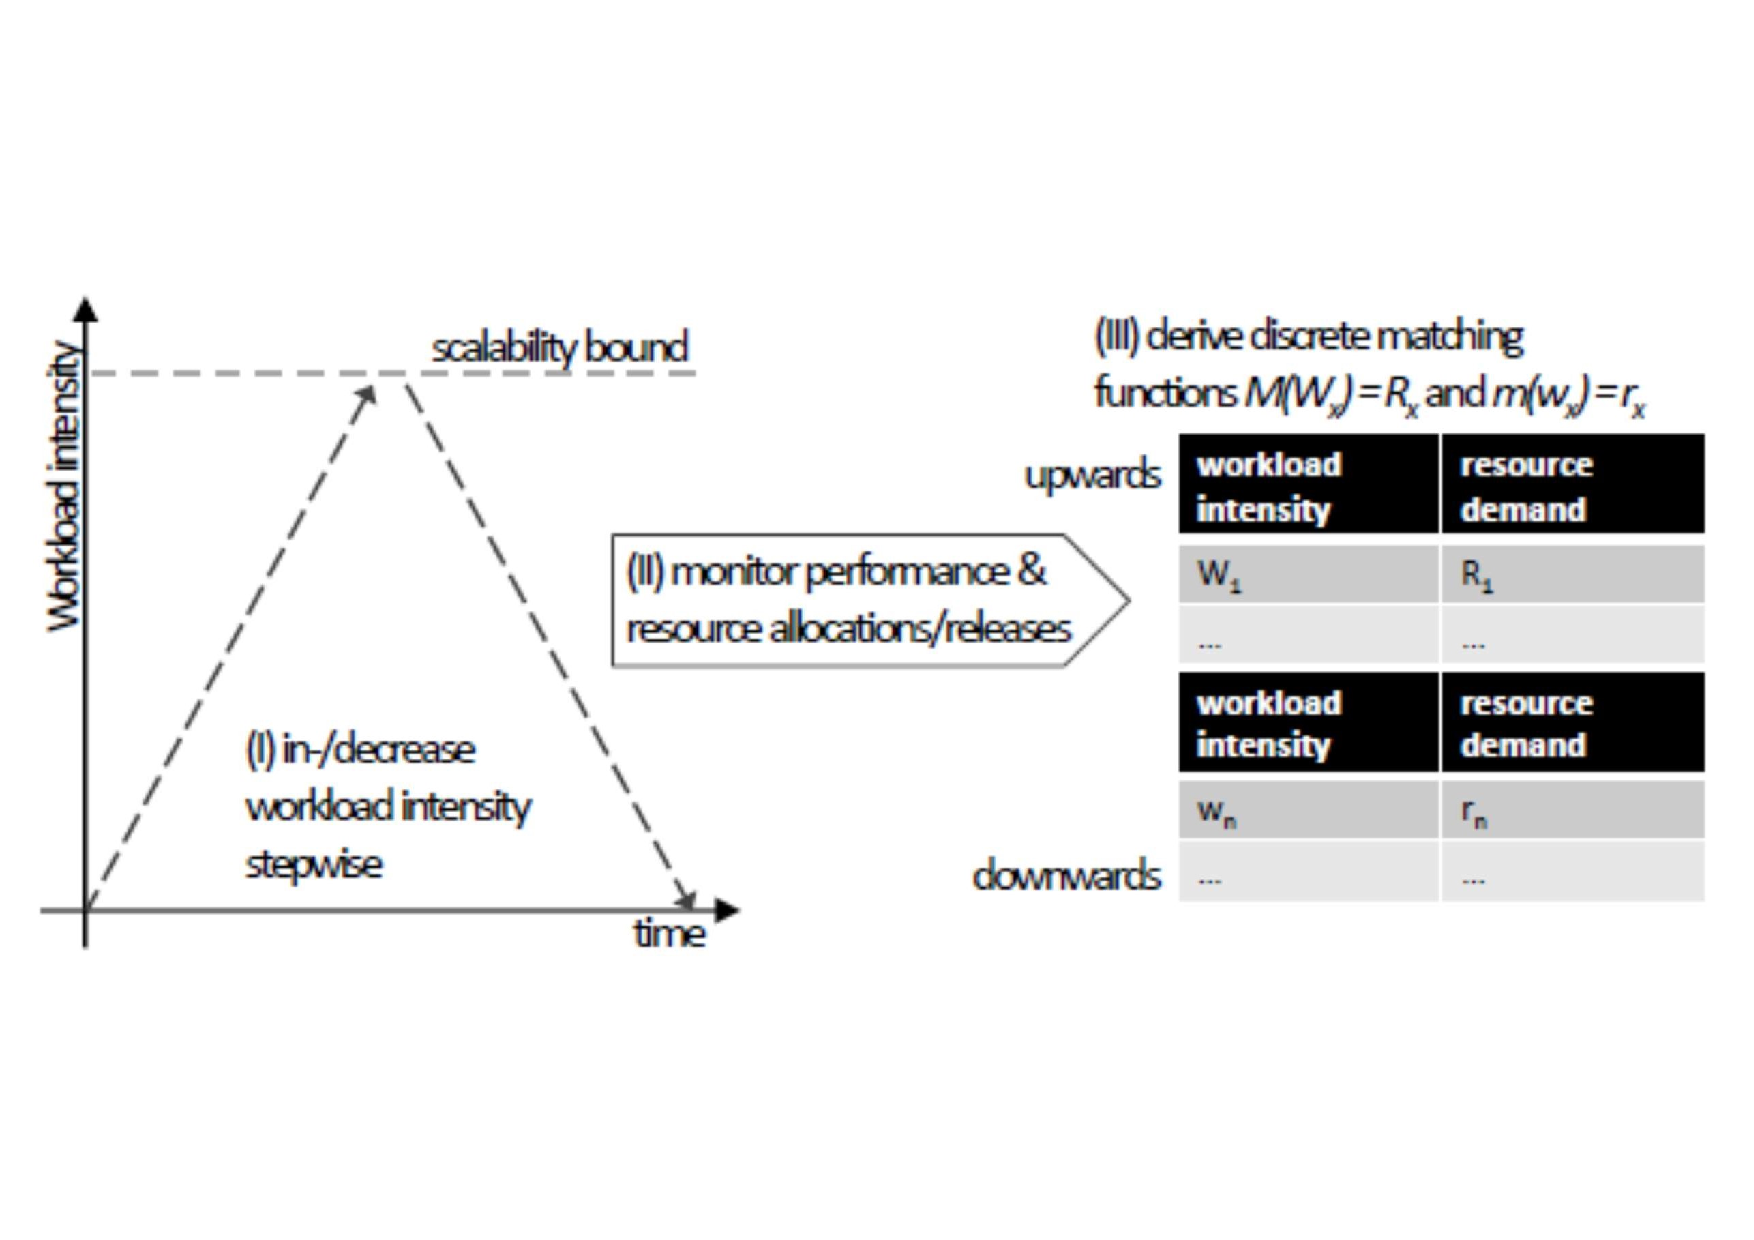
\includegraphics[width=\columnwidth]{Images/elasticity_matching_function.pdf}
	\caption[Elasticity Matching Function derivation.]{Elasticity Matching Function derivation.}
	\label{fig:elasticity_matching_function}
\end{figure}
\begin{figure}
	\centering
	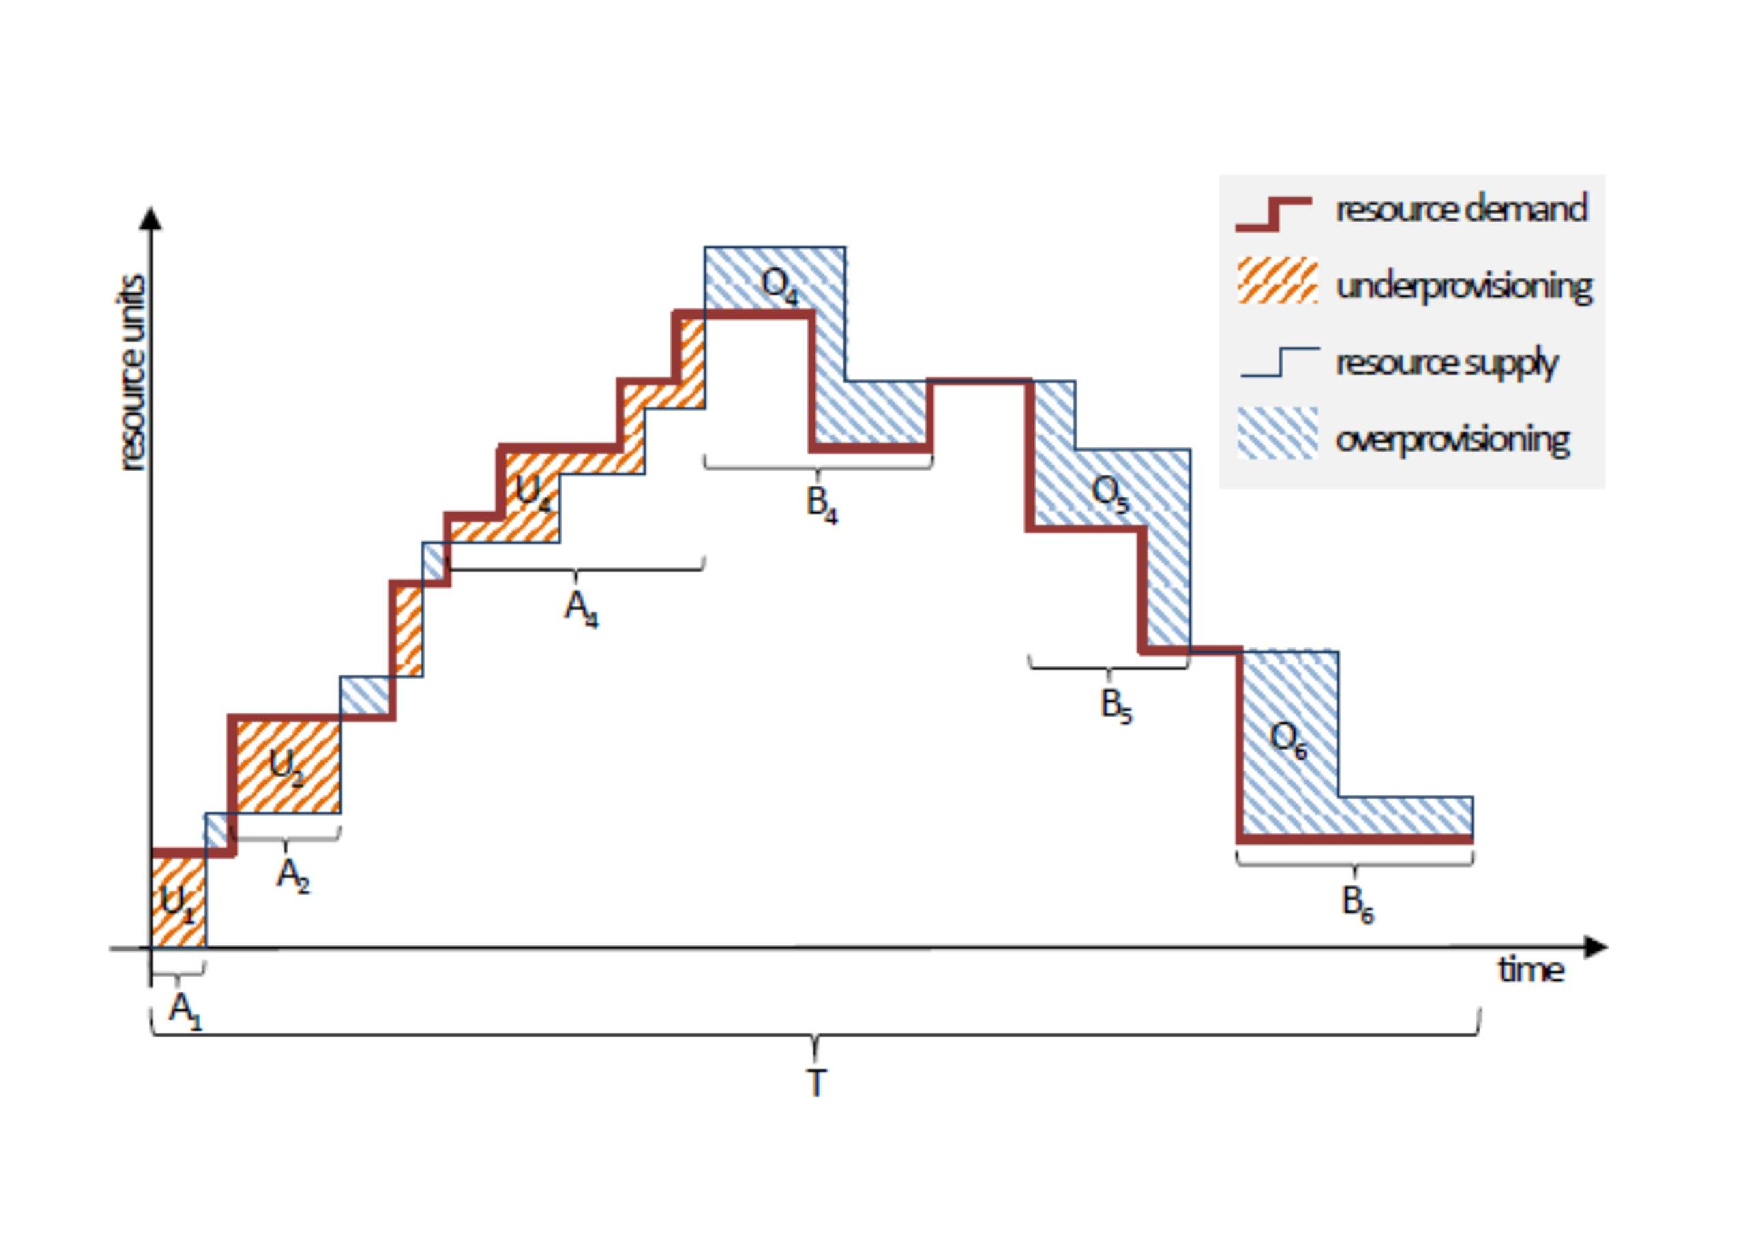
\includegraphics[width=\columnwidth]{Images/elasticity_resource_provisioning_chart.pdf}
	\caption[Resource Provisioning Chart.]{Resource Provisioning Chart.}
	\label{fig:elasticity_resource_provisioning_chart}
\end{figure}

Elasticity reflects the (theoretical) infinite upper bound on resource scalability in cloud computing and the frictionless resource renting model. Nevertheless elasticity is not just a synonym of resource management. Elasticity is also related to trade off between cost and quality~\cite{Dustdar2011}. Cost elasticity describes how resources are managed in response to cost changes, while quality elasticity measures how responsive is the quality to changes in resource utilization.

A \textit{matching function} $m(w) - r$ is a system specific function that gives the minimum quantity of resources r for any given resource type needed to meet the system’s performance requirements at a certain workload intensity. A matching function is required for both up and down scaling directions.

The matching functions can be determined based on measurements, as illustrated in \MyFig{fig:elasticity_matching_function}, by increasing the workload intensity w stepwise, and measuring the resource consumption r, while tracking resource allocation changes. The process is then repeated for decreasing w. After each change in the workload intensity, the system should be given enough time to adapt its resource allocations reaching a stable state for the respective workload intensity. As a rule of thumb, at least two times the technical resource provisioning time is recommended to use as a minimum. As a result of this step, a system specific table is derived that maps workload intensity levels to resource demands, and the other way round, for both scaling directions within the scaling bounds.

An example of how \textit{speed} and \textit{precision} affect resource provisioning is shown in \MyFig{fig:elasticity_resource_provisioning_chart}.


\section{Spark Resource Provisioning}\label{sec:spark_resource_provisioning}
It's important to remember that the cluster manager is responsible for starting executor processes and determine where and when they will run. Using Spark’s embedded cluster manager might be a problem in terms of resource utilization when we want to execute different distributed applications at the same time. Using a single cluster manager for different distributed applications has the advantage of providing a global view on which applications are running and which we want to execute inside the cluster.
Without a single cluster manager, we can have two main approaches
in order to perform resource sharing and allocation:
\begin{itemize}
	\item  allowing every application to allocate all the resources in the cluster at the same time, this leads to an unfair situation of resource contention
	\item splitting the resource pool into smaller pools, one per application.
\end{itemize}
In this way we will avoid resource contention but we will
have a less efficient utilization of the resources, because some of
the applications might request more resources than the ones in
the pool, meanwhile some others are using less resources than
the allocable ones in order to execute.
A more dynamic way of allocating resources will led to a better resource
utilization. Spark natively support executing on top of Apache
Hadoop YARN and Apache Mesos cluster managers.
Spark supports the dynamic allocation of executors, also known as
elastic scaling, this feature allows to add and remove Spark executors
in a dynamic way in order to match the workload.
In traditional static allocation, a Spark application would allocate
CPU and memory upon starting the execution, disregarding how
much resources will effectively use later on. With dynamic allocation
instead it is possible to allocate as much resources as they are
necessary, in order to avoid wasting them. The number of running
executors is scaled up and down according to the workload, in particular
idling executors are removed and when there are tasks waiting
to be executed and new executors are launched. Dynamic allocation can 
be activate in Spark settings and should be used together with the
External Shuffle Service, in this way data that have been manipulated
from the executor is still available after the removal of the executor.
Dynamic allocation has two different policy for scaling the executors:
\begin{itemize}
	\item Scale Up Policy: new executor are requested when there are
	pending tasks, the number of executors is increased exponentially
	because they start slow and so the application might need
	a slightly higher number of them
	\item Scale Down Policy: idling executors are removed after a certain
	amount of time, this amount of time can be configured
\end{itemize}
In order for dynamic allocation to work, we must configure it, by setting
the initial number of executors that are created when application
starts and the minimum and maximum number of executors that can
be reached when scaling down and up respectively. Dynamic allocation
is available on all cluster managers currently supported by Spark,
even in Standalone mode.

\subsection{Apache Hadoop Yarn}\label{sec:hadoop_yarn}
Apache Hadoop YARN (Yet Another Resource Negotiator) is the next
generation of Hadoop’s compute platform\cite{Vavilapalli:2013:AHY:2523616.2523633}. 
\begin{figure}
	\centering
	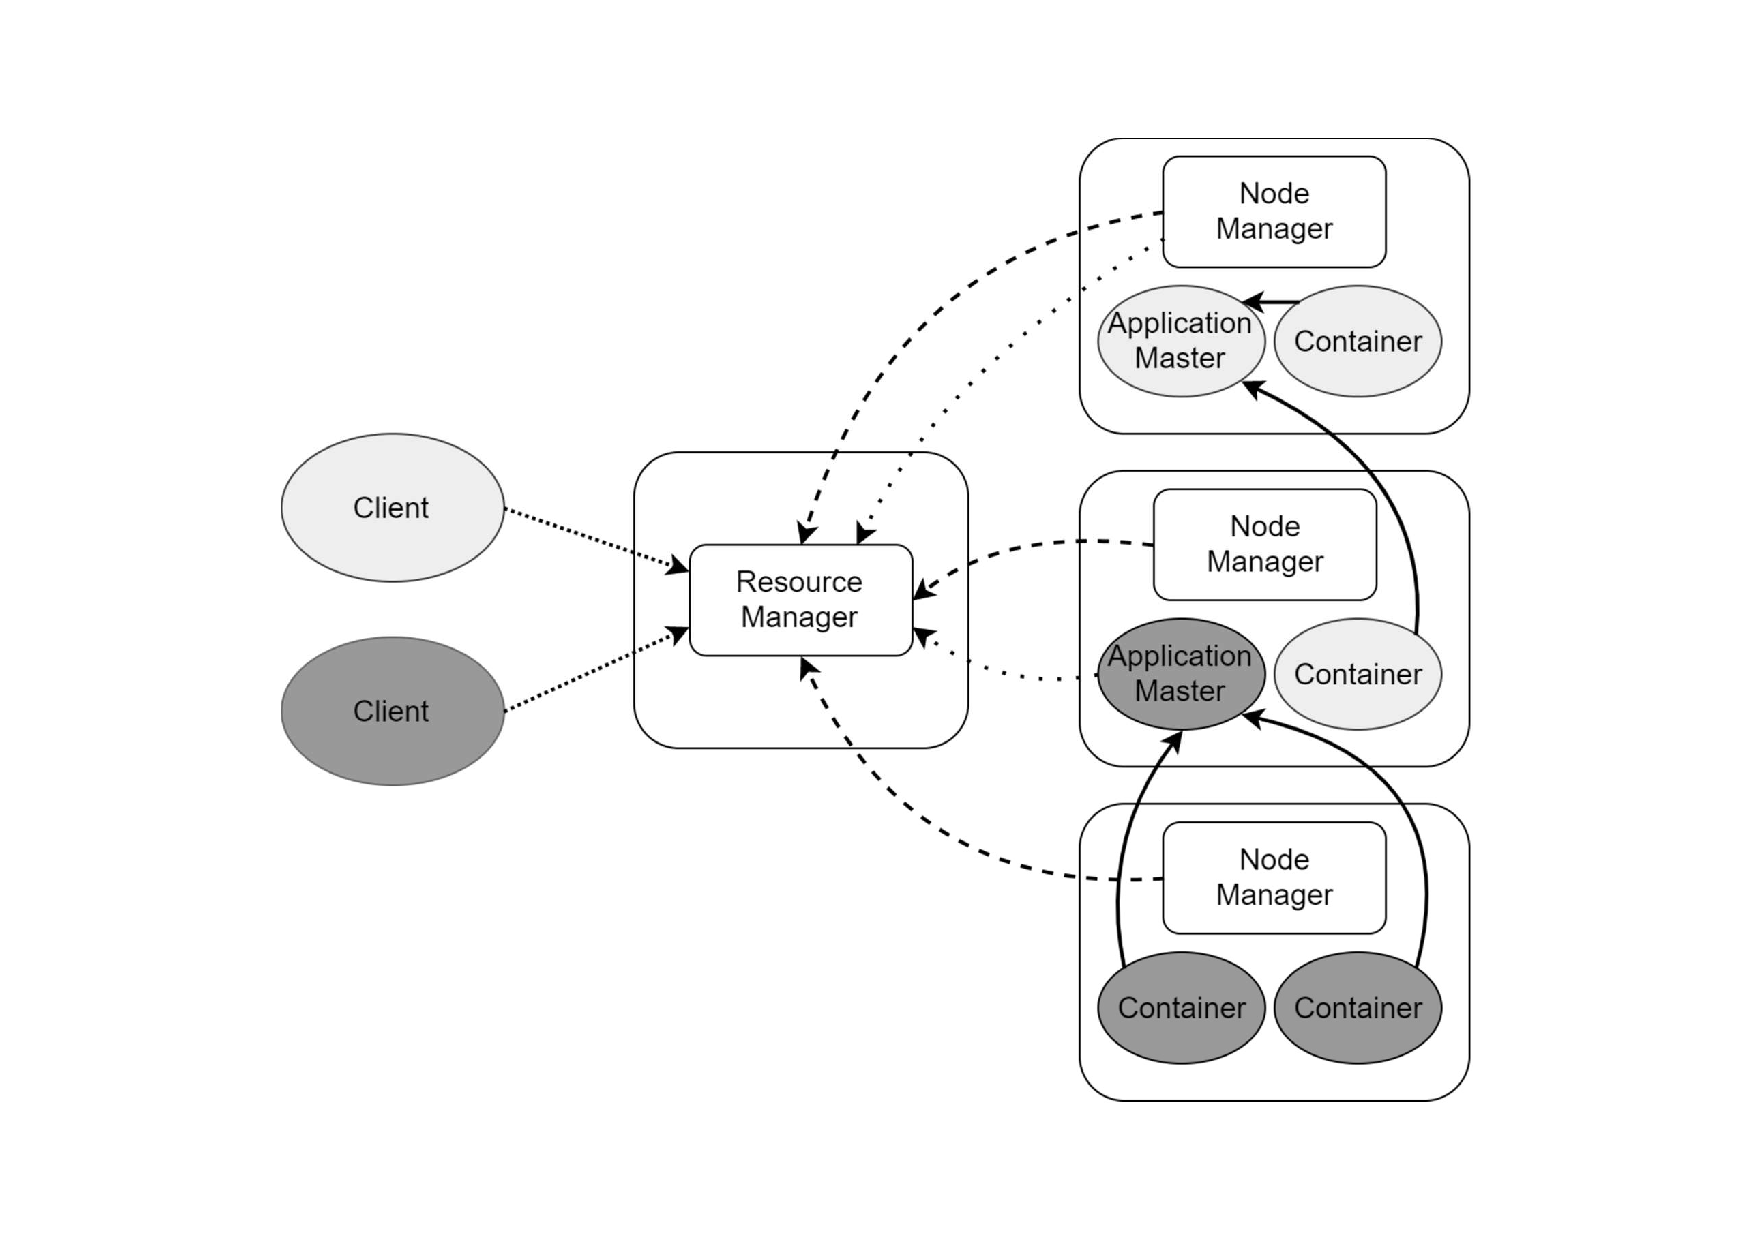
\includegraphics[width=\columnwidth]{Images/apache_hadoop_yarn_architecture.pdf}  
	\caption[Apache Hadoop YARN Architecture]{Apache Hadoop YARN Architecture.}
	\label{fig:apacheHadoopYarnArchitecture}
\end{figure}
The idea is to split
the functionality of resource management and job scheduling and
monitoring. This is achieved by having two different kind of daemons
running, one global Resource Manager (RM) and a per-application
Application Master (AM).
Resource Manager (RM) and Node Manager (NM) form the data
computation framework (Figure 1.4). RM is the authority that manages
resources among all the applications that are running in the
system, meanwhile NM is the per-machine daemon who is responsible
for managing containers, monitoring and reporting. The perapplication
AM has the goal of negotiating resources with RM and
working with NM in order to execute and monitor tasks.
Resource Manager (RM) is composed by two components: Scheduler
and Applications Manager.
The Scheduler is responsible for allocating resources to the various
applications that are running, by taking into account constraints
about capacity, queues, etc. It is a real scheduler in the sense that
it does not perform monitoring or tracking of the application state.
Moreover, it does not offer any guarantee that a failed application will be reexecuted
after an application or hardware failure. The Scheduler performs
the allocation according to the resources that are requested by
an application; this is based on the abstract notion of container which
has elements as memory, CPU cores, disk and network bandwidth.
There are pluggable policy that determine the repartition of resources
among the different applications, for example we have the Capacity
Scheduler, designed for multi-tenant clusters, and the Fair Scheduler,
that shares cluster resources fairly.
The Applications Manager is responsible of accepting the submission
of a job, it negotiates the first container that will execute the AM and
it offers a service that can be used to restart the AM in case of failure.
The per-application AM has the goal of negotiating the needed
containers from the Scheduler, track their status and monitor their
progress.
The RM keeps a global model of the cluster state and thanks to the
resource requirements reported by the running applications, it makes
possible to enforce a global scheduling, but it is required to have an
accurate understanding of the applications’ resource requirements. In
response to AM requests, the RM generates containers together with
tokens that grant access to resources. An extension of the protocol
allows the RM to ask back resources from applications, for example
when cluster resources become scarce.
Application Master (AM) is the process that coordinates the execution
of an application inside the cluster. It is important to remember
that AM itself is run in the cluster, just like any other container. Periodically,
an heartbeat is sent to the RM in order to confirm its liveliness
and to update the Scheduler about its resource requests. After having
modeled the application requirements, the AM encodes its preferences
and constraints inside the heartbeat message. This information
are stored in the form of Resource Request, containing the desired number of containers (e.g., 100 container), the resources of each container
(e.g., <2 CPU, 2 GB>), the locality preferences and the priority of this
resource request with respect to the other ones of this application.
When a container lease is received, the AM can choose to modify its
execution plan in order to take into account the abundance or scarcity
of resources.
Node Manager (NM) is the worker daemon in YARN, its purpose
is to authenticate container lease, manage dependencies, monitoring
the execution of containers and offer them a set of services. After
having registered with the RM, the NM sends heartbeats in order to
communicate its status and receives instructions from the RM. All
the containers are described by a container launch context (CLC), that
keeps track of all the environment variables, the dependencies, the security
tokens, but also of the payloads needed by NM services and the
commands that are needed to launch the process inside the container.
After having validated the authenticity of the container lease, the NM
configures the container with the specified resource constraints and
initializes a monitoring subsystem. In order to launch the container,
dependencies are copied into local storage. NM also has the duty of
killing container upon a request from RM or AM, for example when a
tenant is being evicted or when an application completes. Whenever
a container exits, NM needs to clean the working directory. When an
application ends, all the resources held by its container on all nodes
are released. NM periodically checks the state of the physical machine
and informs the RM of a possible unhealthy state.
\subsection{Apache Mesos}\label{sec:apache_mesos}
Apache Mesos is an open-source project used to manage computer
clusters. 
\begin{figure}
	\centering
	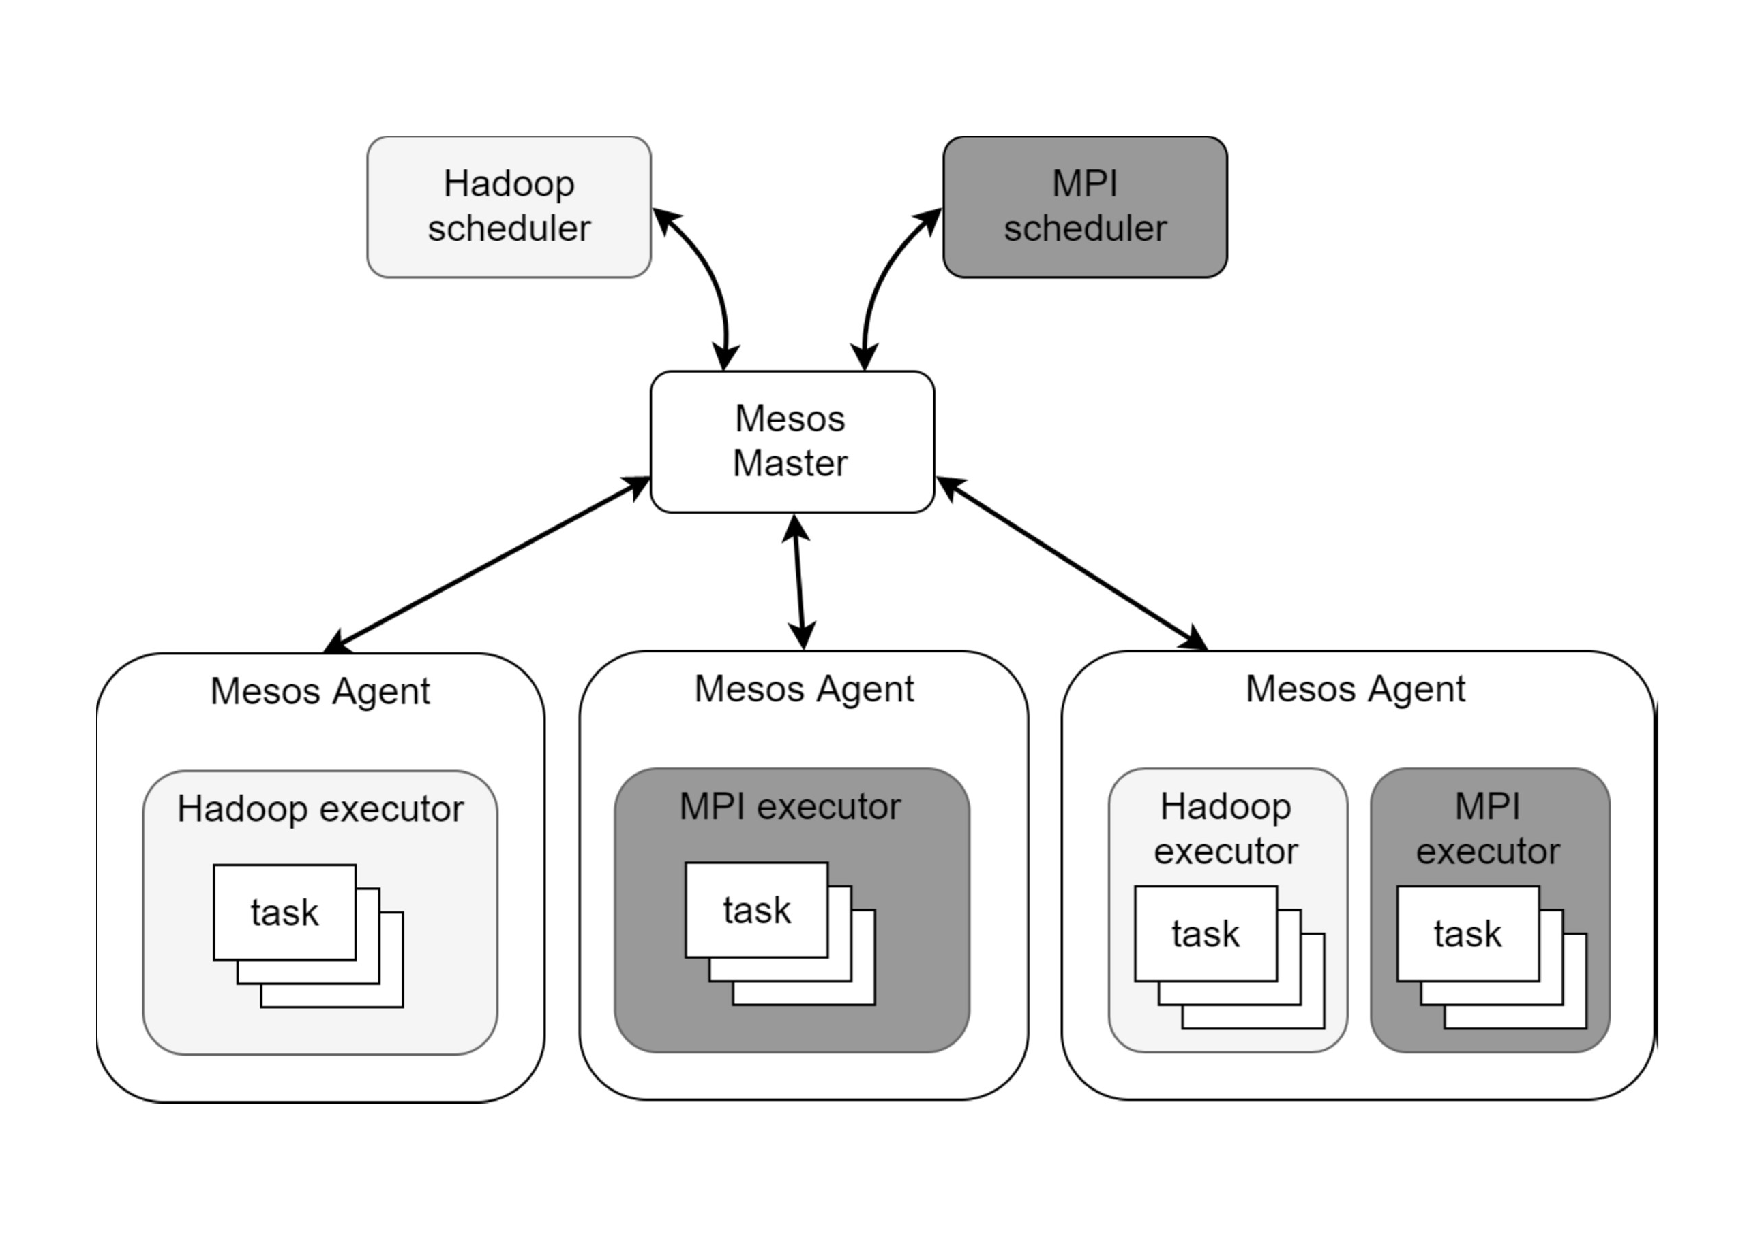
\includegraphics[width=\columnwidth]{Images/apache_mesos_architecture.pdf}  
	\caption[Apache Mesos Architecture]{Apache Mesos Architecture.}
	\label{fig:apacheMesosArchitecture}
\end{figure}
The purpose of Mesos is to share cluster between different
computing frameworks, such as Apache Hadoop or Message Passing
Interface (MPI). The sharing increments the utilization of the cluster
and prevents per-framework data replication. 
Mesos shares resources
in a fine-grained way, allowing to achieve data locality. It presents
a scheduling mechanism on two layer called resource offers. Mesos
decides how many resources to offer to each of the running frameworks,
meanwhile they decide how many resources to accept and
which computation to execute on the granted resources.
New cluster computing frameworks continue to emerge, it is clear
that finding a framework that is optimal for all type of application
is almost impossible. We expect that organization would like to use
different frameworks inside the same cluster, picking the best one according
to the kind of application that they are going to execute. Two
classic solution are: i) statically partitioning the cluster and executing
one framework per partition; ii) allocate a set of VMs to each of the
frameworks. Unluckily these solution do not achieve high utilization
and efficient data sharing. The main problem is the different allocation
granularity of these solutions and the one of the existing frameworks,
for example Hadoop employs a fine grained resource sharing
model, where nodes are divided into slots and each job is composed
by short tasks that match the slots.
\begin{figure}
	\centering
	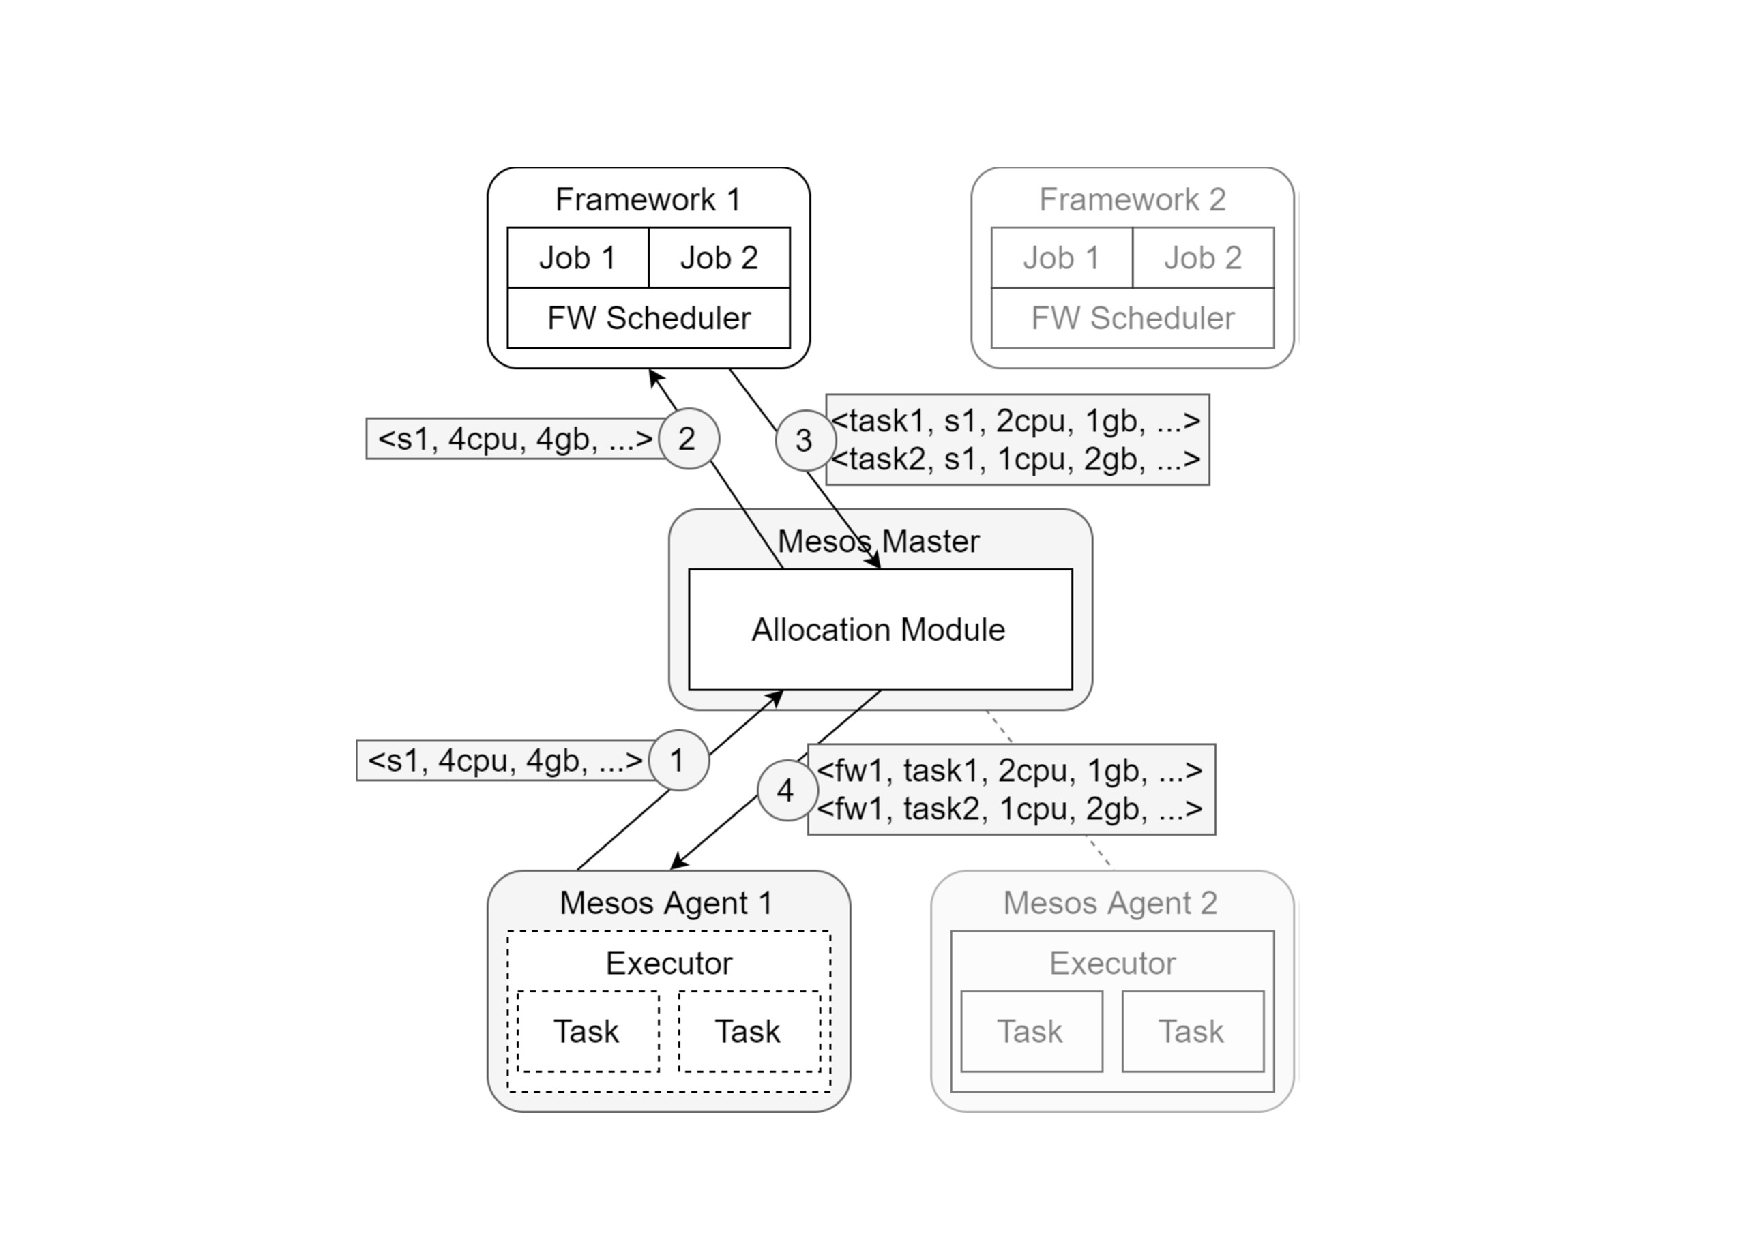
\includegraphics[width=\columnwidth]{Images/apache_mesos_resource_offer_example.pdf}  
	\caption[Apache Mesos Resource Offer Example]{Apache Mesos Resource Offer example. 1) Mesos Agent 1 reports
		free resources to the Allocation Module; 2) Allocation
		Module offers resources to Framework 1 scheduler; 3) Framework
		1 scheduler accepts resources and assign tasks; 4) Allocation
		Module launches tasks on the executor running in Mesos
		Agent 1.}
	\label{fig:apacheMesosResourceOfferExample}
\end{figure}
The presence of short tasks allows
us to achieve high utilization, as jobs can rapidly scale when
new nodes are available. But it is not possible to achieve fine grained
sharing across frameworks, because they have been developed in an
independent way, and thus it is difficult to efficiently share the cluster
among different frameworks.
Mesos delegates the control over the scheduling to the different
frameworks. In this way it is possible to have the abstraction of the
resource offers, that encapsulate a bundle of resources that the framework
can allocate on a node in order to execute a task. Mesos decides
how many resources to offer to each framework, this is based on
policies, and the framework decides which resources to accept and
which tasks to execute on them. Even though this approach does not
lead to a globally optimum scheduling, it has been proved that it performs
particularly well in practice, allowing the frameworks to obtain
near perfect data locality. Mesos provides other benefits to its users,
for example the possibility of running different instances of the same
framework or even different versions.
Mesos is composed by a master process that manages slave daemons
running on each cluster node and frameworks that run tasks
on these slaves, as we can see from \myFig{fig:apacheMesosArchitecture} . Master implements
fine-grained sharing across frameworks using resource offers. Every
resource offer is a list of free resources on the different slave nodes.
The master decides how many resources to offer to each framework,
according to some policy such as fairness or priority. 

Apache Mesos Resource Offer example. 1) Mesos Agent 1 reports
free resources to the Allocation Module; 2) Allocation
Module offers resources to Framework 1 scheduler; 3) Framework
1 scheduler accepts resources and assign tasks; 4) Allocation
Module launches tasks on the executor running in Mesos
Agent 1.

Every framework that is running on Mesos is composed by two components: a
scheduler, that registers with the master in order to obtain the resource
offers, and an executor process that is launched on the slave
node in order to execute framework’s tasks. While the master chooses
how many resources to offer, the scheduler chooses which resources
to use among those offered. When an offer is accepted, the scheduler
sends to the master the description of the tasks that should be
executed. The resource offer process is repeated every time tasks are
finished and when there are new free resources. In order to maintain
a light interface, Mesos does not ask the frameworks to specify
their resource requirements or constraint, instead it gives them the
possibility of refusing offered resources. Mesos allows frameworks to
set up a set of filters, in the form of boolean predicates, specifying
the conditions on which the framework will always refuse a proposal
(e.g., providing a whitelist of nodes it can run on).
In Figure 1.6 we have an example of resource offer process.
1. Agent 1 reports to master that it has 4 CPUs and 4 GB of memory
free. Master invokes its allocation module policy, which tells
that framework 1 should be offered all the resources.
2. Master sends a resource offer describing the resources available
on agent 1 to framework 1.


\subsection{Spark on Yarn}{subsec:sparkOnYarn}
Support for running Spark on YARN was added to Spark in version
0.6.0 and has been improved in subsequent releases~\cite{misc:SparkOnYarn}.
When running on YARN, each Spark executor is run inside a YARN
container. Spark supports two different modes to run on YARN, the
Yarn-cluster and Yarn-client mode.
In client mode, as shown in \myFig{fig:sparkOnYarnClientMode}, the driver program is run
inside the client process. In this way, the Application Master (AM) that
is run in a YARN container is used only to request resources to the Resource
Manager (RM). This mode is useful for interactive applications
and for debugging purposes, since you can see applications’ output
immediately on the client side process. If the client disconnects from
the cluster, the Spark application will terminate, this is due to the fact
that the driver process resides on the client.
In cluster mode instead, as shown in Figure 1.10, Spark driver program
is run inside the AM process managed by YARN. After initializing
the application, client can disconnect from the cluster and reconnect
later on. This mode makes sense when using Spark on YARN in
production jobs.
Running on top of YARN cluster manager has some benefits. First
of all YARN allows to dynamically share the cluster resources between
the different frameworks that are running together. For example
we can run MapReduce jobs after running Spark jobs without the
need of changing YARN configurations. Moreover, YARN supports
for categorizing, isolating and prioritizing workloads and employs
security policies, in this way Spark can use secure authentication between
its processes.
\begin{figure}
	\centering
	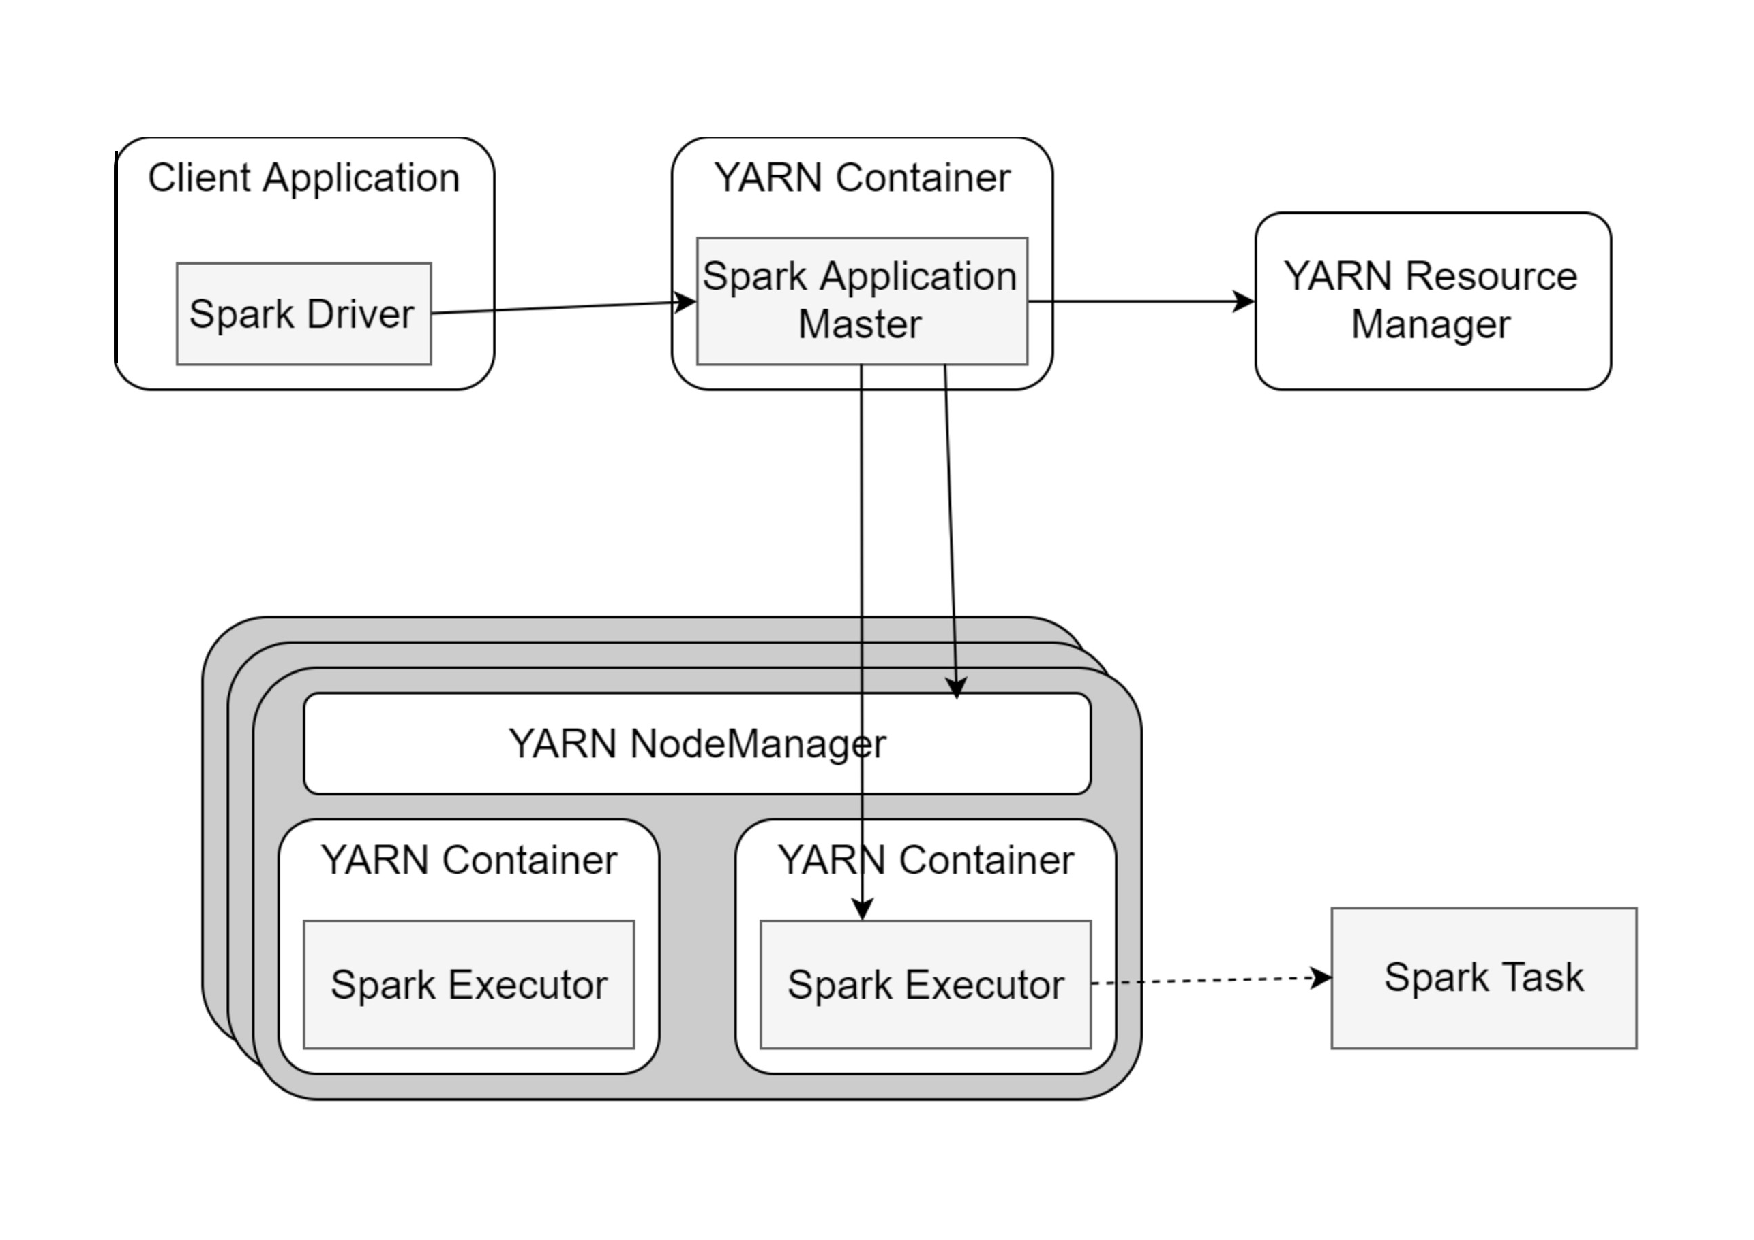
\includegraphics[width=\columnwidth]{Images/spark_yarn_client_mode.pdf}  
	\caption[Spark on YARN Client Mode]{Spark on YARN Client Mode.}
	\label{fig:sparkOnYarnClientMode}
\end{figure}
\begin{figure}
	\centering
	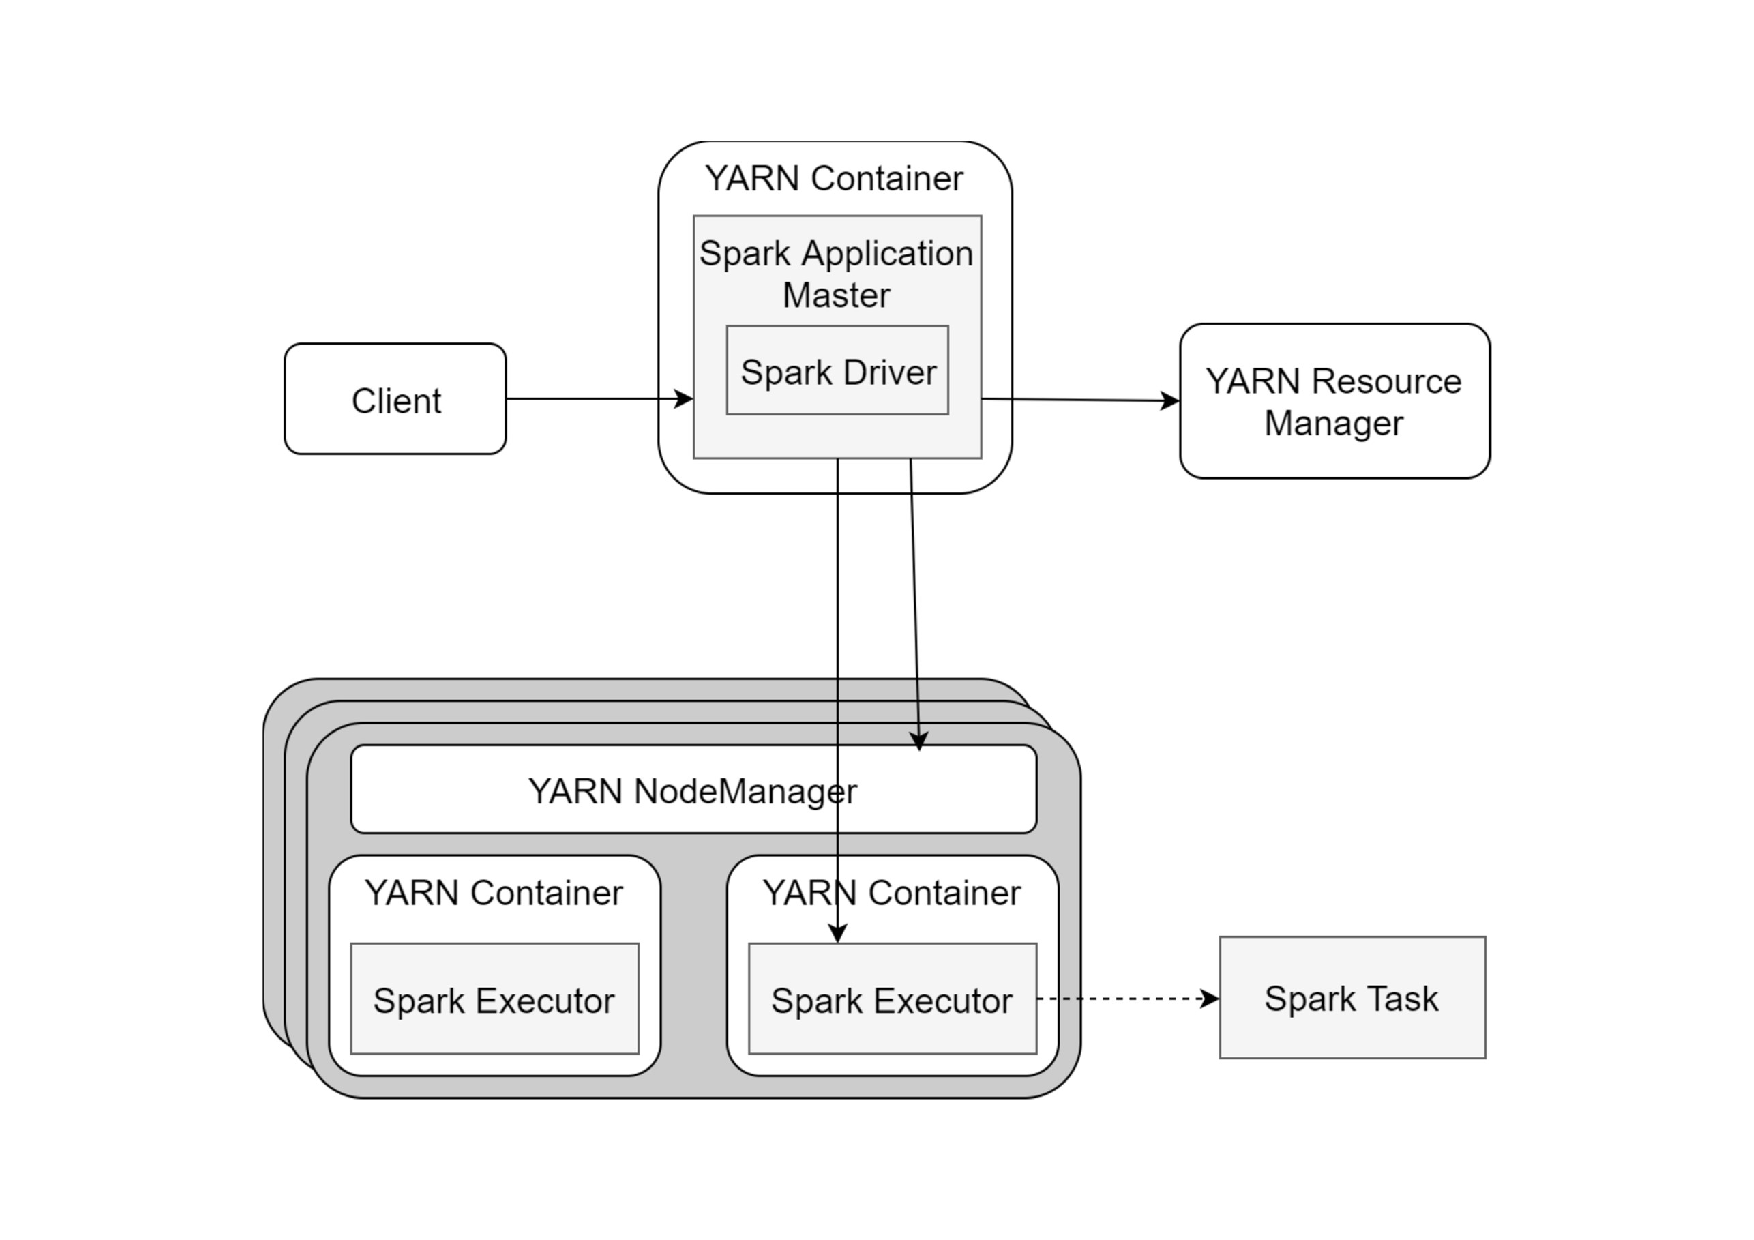
\includegraphics[width=\columnwidth]{Images/spark_yarn_cluster_mode.pdf}  
	\caption[Spark on YARN Cluster Mode]{Spark on YARN Cluster Mode.}
	\label{fig:sparkOnYarnClusterMode}
\end{figure}
\begin{figure}
	\centering
	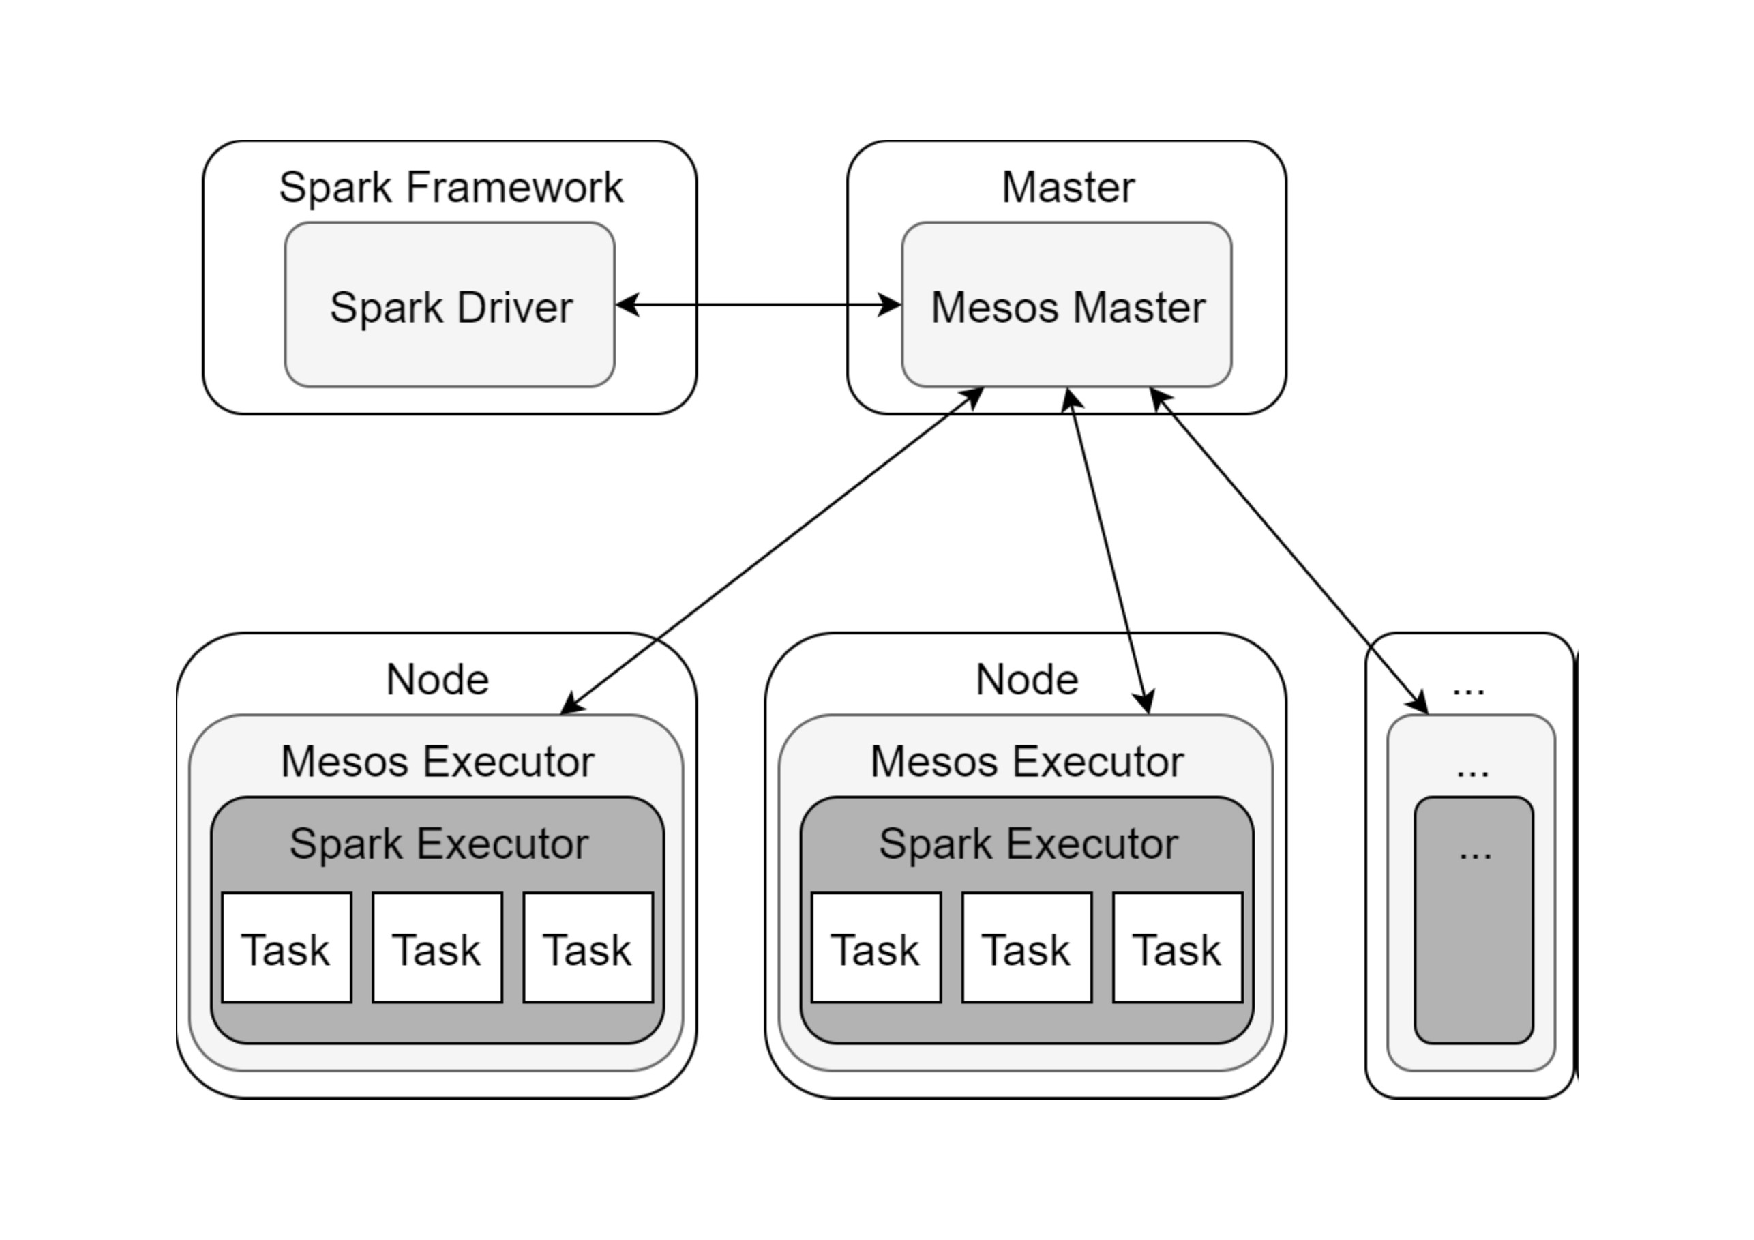
\includegraphics[width=\columnwidth]{Images/spark_mesos_coarse_grained_mode.pdf}  
	\caption[Spark on Mesos Coarse Grained Mode]{Spark on Mesos Coarse Grained Mode.}
	\label{fig:sparkOnMesosCoarseGrainedMode}
\end{figure}
\begin{figure}
	\centering
	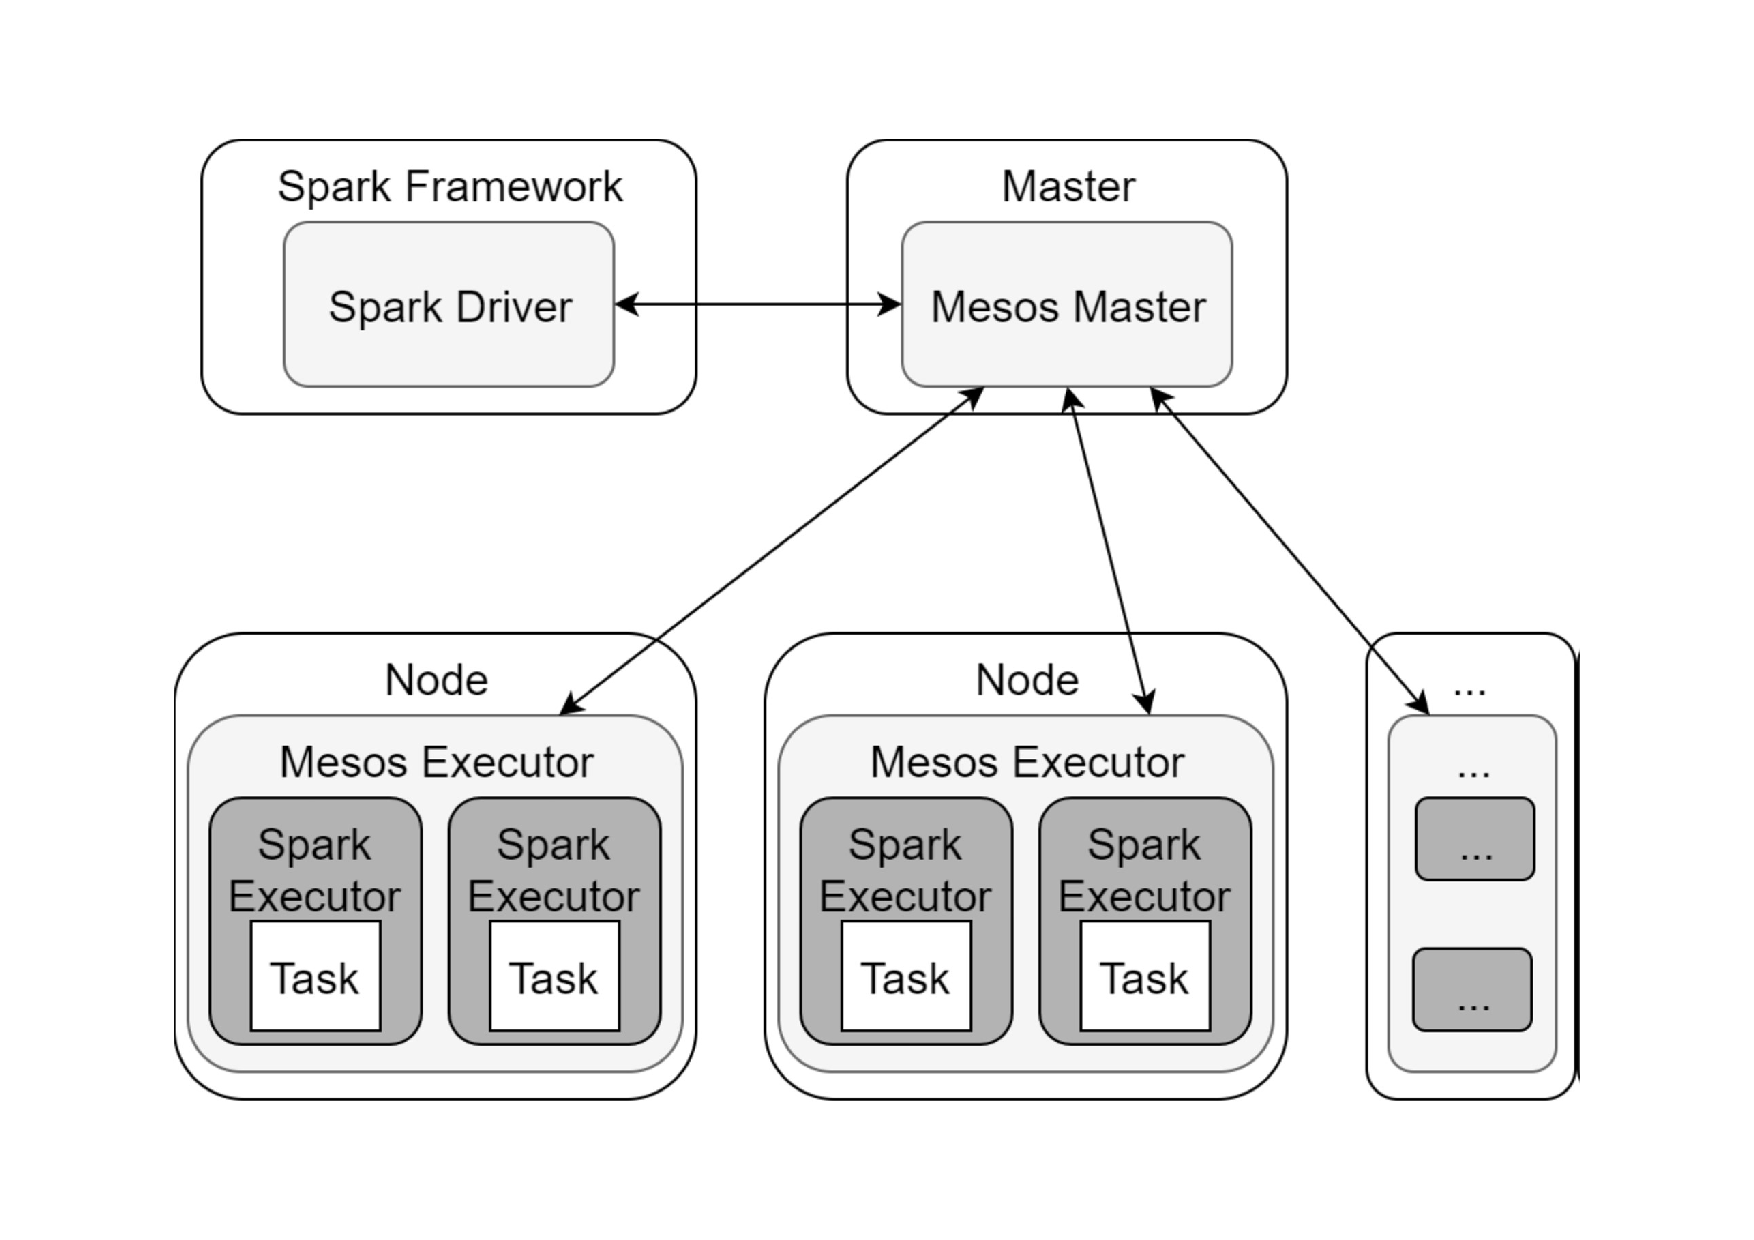
\includegraphics[width=\columnwidth]{Images/spark_mesos_fine_grained_mode.pdf}  
	\caption[Spark on Mesos Fine Grained Mode]{Spark on Mesos Fine Grained Mode.}
	\label{fig:sparkOnMesosFineGrainedMode}
\end{figure}

When running on YARN, Spark executors and driver program use
about 6-10\% more memory with respect to the standalone execution,
this is due to the fact that this extra amount of off-heap memory is
allocated in order to take into account YARN overheads.

\subsection{Spark on Mesos}{subsec:sparkOnMesos}
Support for running Spark on Mesos was added to Spark in version
1.5. Spark on Mesos can be executed in two different modes: coarse-grained
and fine-grained \cite{misc:SparkOnMesos}.
In coarse-grained mode, as shown in \myFig{fig:sparkOnMesosCoarseGrainedMode}, 
each Spark application is submitted to Mesos master as a framework and Mesos
slaves will run tasks for the Spark framework that are Spark executors.
Mesos tasks are launched for each Spark executor and those
Mesos tasks stay alive during the lifetime of the application unless
we are using dynamic allocation or the executor is killed for various
reasons. The advantage of coarse-grained mode is in a much lower task
startup overhead, with respect to the other mode, and so it is good
for interactive sessions.
The drawback is that we are reserving Mesos resources for the complete
duration of the application, unless dynamic allocation is active.
Dynamic allocation allows to add and remove executors based on
load: i) kill executor when they are idle, ii) add executors when tasks
queue up in the scheduler. To use dynamic allocation it is required
that the external shuffle service is running on each node.
In fine-grained mode, shown in \myFig{fig:sparkOnMesosFineGrainedMode}, 
Mesos tasks are launched for each Spark task, and those tasks die as soon as Spark tasks are done. This mode has too much overhead in case that Spark has too
many tasks, for example if Spark application has 10,000 tasks, then
Spark needs to be installed 10,000 times on Mesos agents. Because
of this huge overhead, fine-grained mode has been deprecated since
Spark version 2.0.0. This mode allows multiple instances of Spark to
share cores at a very fine granularity, but it comes with an additional
overhead in launching each task. Thus this mode is inappropriate
for low-latency requirements like interactive queries or serving web
requests, instead it is fine for batch and relatively static streaming.
Similarly to what happens on YARN, it is possible to run spark in
Mesos-client or Mesos-cluster mode. In client mode, the driver process
is executed in the client machine that submits the job, so it is required
that it stays connected to the cluster for the entire time of the application
execution. In cluster mode instead, the driver program is run on
a machine of the cluster.

\section{Virtualization and Containerization}
Virtualization refers to creating the virtual version of something, included
hardware components, storage devices and computer networks.
Virtualization is born in 1960's, as a way to logically partition the system
resources offered by a mainframe computer between many different
applications. From this point, the meaning of the word has been
widely extended.
Virtualization is a technology that allows creating multiple simulated
environments or dedicated resources from a single unique physical
hardware system. An hypervisor is a software that can directly
connect to the hardware, with the purpose of splitting the unique
physical system into separated environments, different from each other 
and secure, known as virtual machines (VM's). These VM's rely on
the hypervisor ability to separate the hardware resources and distribute
them in a proper way.
The original physical machine equipped with the hypervisor is
called host, meanwhile the VM's are called guests. These guests use the computation resources, such as CPU, memory and storage, as a set of resources that are easily re-allocatable. The operators can control the virtual instances of CPU, memory, storage
and other resources, so that the guests can receive all the resources they need
to execute their task. The words host and guest are used to distinguish the software that runs on the physical hardware from the software that is running on the virtual machines.
Hardware virtualization or platform virtualization refer to the creation
of a VM that acts like a real computer with an OS. The software
that is run in this VM is separated from the underlying hardware.
This allows us to run particular configurations, for example we run a
computer with a Windows OS that hosts a VM with Linux as guest OS.
There are at least two different hardware virtualization types:
\begin{itemize}
	\item full virtualization: it completely simulates the hardware in order
	to allow the software, typically a guest OS, to be run without the
	need of modifications
	\item paravirtualization: the hardware environment is not simulated,
	anyway guest programs are run in isolated domains, as if they
	were run in completely separated systems. Guest programs need
	to be modified in a specified way in order to run in this kind
	of environment.
\end{itemize}
\begin{figure}
	\centering
	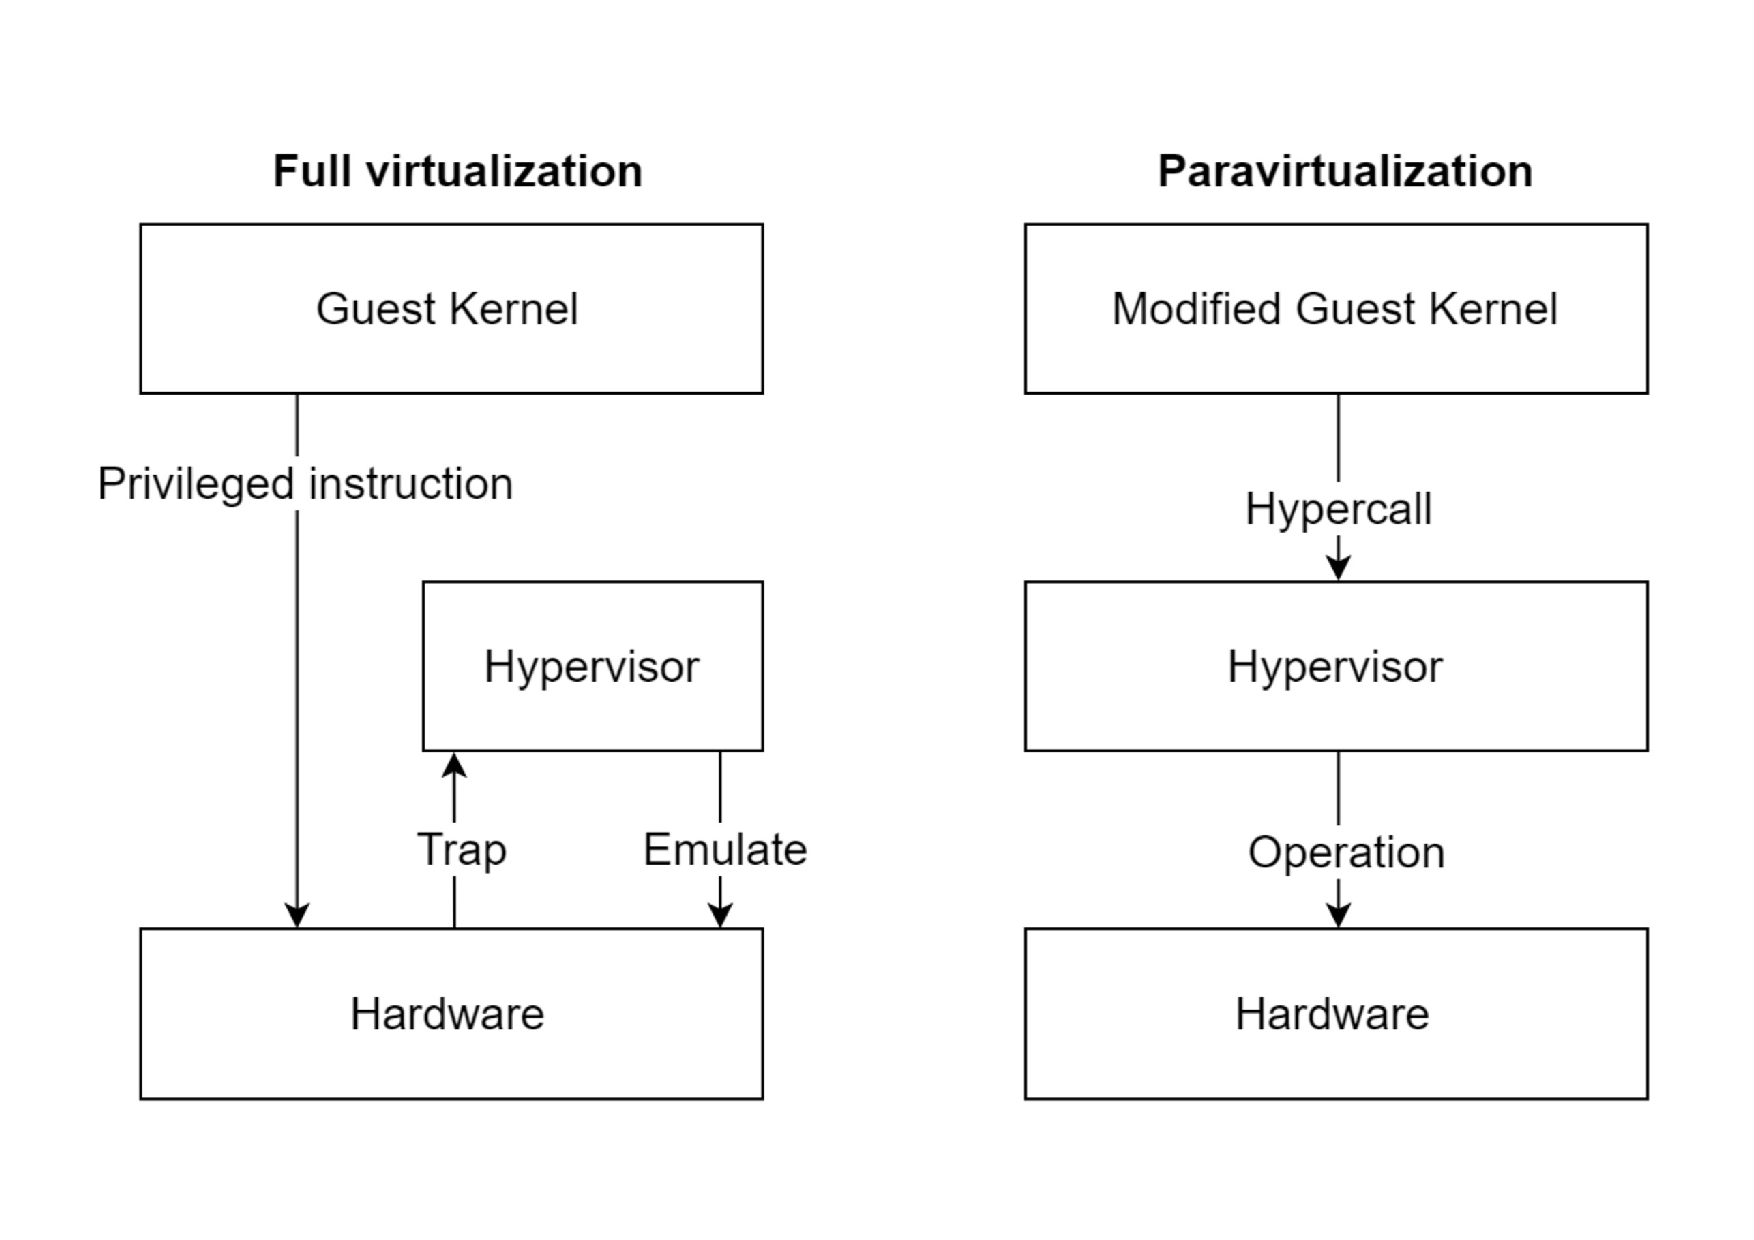
\includegraphics[width=\columnwidth]{Images/virtualization_paravirtualization.pdf}  
	\caption[Full virtualization and paravirtualization]{Full virtualization and paravirtualization.}
	\label{fig:virtualizationParavirtualization}
\end{figure}
In \myFig{fig:virtualizationParavirtualization}, we can see the differences between the two kind
of virtualization. In paravirtualization, the VM presents a different
interface compared to the one of a physical machine. This requires
modification in the guest OS in order to allow its execution inside
the VM. The hypervisor exposes a set of APIs that the guest OS must
use to execute privileged instructions. Calls to these particular functions are often defined as Hypercalls. In full virtualization instead, VM have the same interface as the physical ones. Ideally, the guest OS would not be able to determine if it is being
run on a physical or virtual machine. The great advantage of full
virtualization is that we do not need to modify the OS. In this way
the hypervisor can adopt a trap system to execute privileged
instructions. We can improve the efficiency of the virtualization by using hardware assisted virtualization, in particular we can decide to use CPU's that
provide efficient support for virtualizing on hardware, but also other
kind of hardware components that can improve the performance of
the guest environments.
Hardware virtualization can be seen as a trend of the enterprise IT
that includes autonomic computing, a scenario in which the different
environments are able to manage themselves based on the detected level of 
activity, and utility computing, where the processing power is seen
as a utility that users pay only when needed. The purpose of virtualization
is to centralize the administrative tasks, offering scalability and
good resource utilization. With virtualization, different OS can run
in parallel on a single CPU. This parallelism reduces overhead cost
in a way different from multitasking, where different
programs are executed in parallel on the same OS. 
Thanks to virtualization, an enterprise IT can better handle updates and rapid changes in OS and applications, with little impact on users. Virtualization allows organizations
to have better efficiency and availability of resources and
applications.
It is important to remember that hardware emulation is a complete
different thing from hardware virtualization, in particular with emulation
we have a piece of hardware that imitates another piece of
hardware. In virtualization instead a hypervisor, which is a piece
of software, mimics a piece of hardware or even an entire computer.
Moreover, a hypervisor is not an emulator, even though both are
software programs that mimic hardware, their domain of use is different.
\begin{figure}
	\centering
	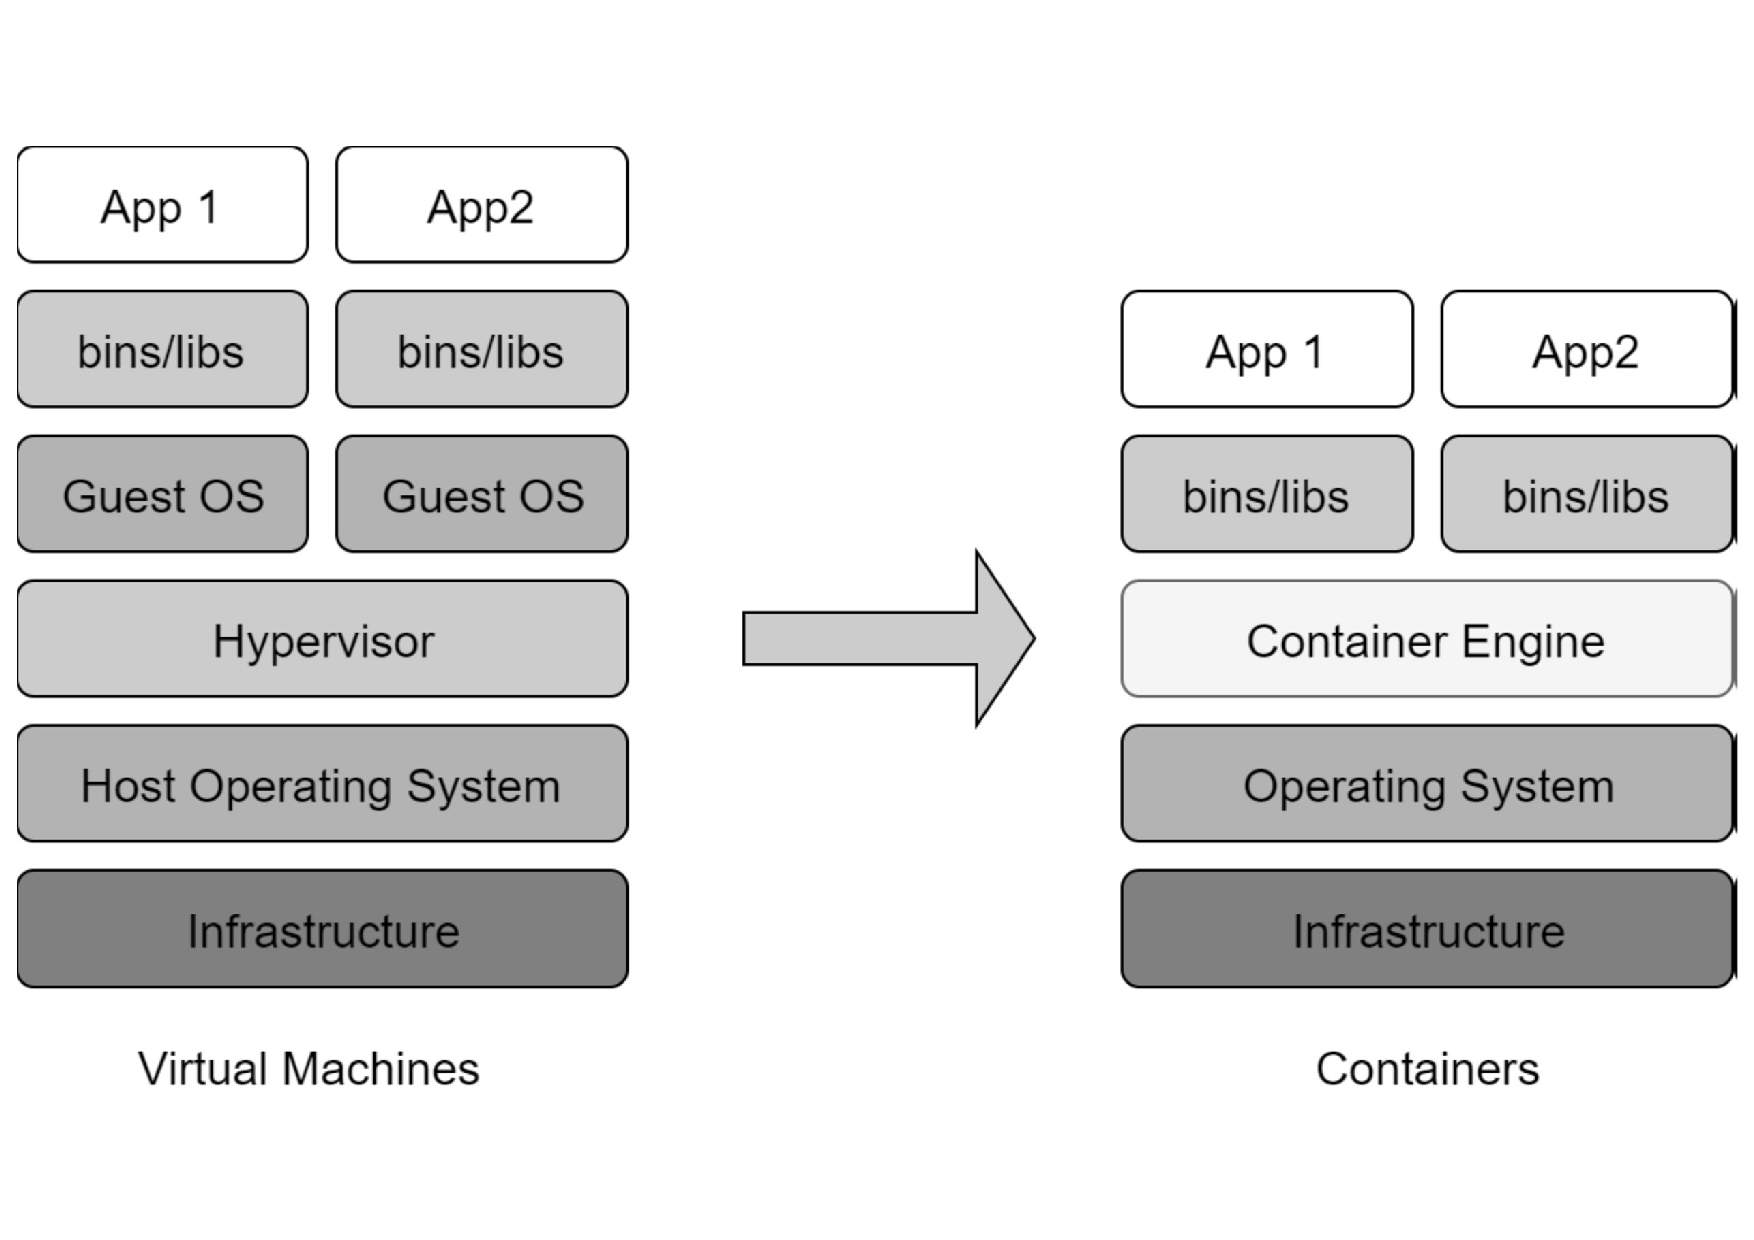
\includegraphics[width=\columnwidth]{Images/vm_vs_container.pdf}  
	\caption[Architecture of virtual machines and containers]{The difference in  architecture between virtual machines and containers.}
	\label{fig:vmVsContainer}
\end{figure}
Containerization is a OS-level virtualization technique that allows
deploying and executing distributed applications without the need
of launching an entire VM for each of the applications (\myFig{fig:vmVsContainer}).
These multiple isolated systems are called containers. They are executed
on top of a single host controller and access a single kernel.
Since containers share the same OS kernel of the host, they can be a lot
more efficient than a VM, that instead needs a separate instance of the
OS. Containers own all the different components that are needed in
order to execute the desired software, such as files, environment variables
and libraries. The host OS controls the access of the container to
the physical resources, such as CPU and memory, in order to prevent
a single container from occupying the entire resources offered by the
host.
The main advantages of containerization come from efficiency in
terms of memory, CPU and storage, when compared to traditional
hardware virtualization. Since containers do not have the same overhead
of VM, in particular we do not need different instances of the OS and 
is possible to support more containers on the same infrastructure.
Containerization offers better performances since there is a single OS
that takes care of all the hardware calls. A special advantage 
of the containers is the fact that they can be created much faster than
instances based on an hypervisor. This allows to have a more agile environment and allows the creation of new approaches to virtualization, such as microservices and continuous integration and delivery of services.
Potential disadvantages of containerization are the absence of
isolation from the host OS. Since containers share the same host OS, a
potential security threat might easily gain access to the entire system.
This does not happen when using virtualization based on a hypervisor,
since in this case the only compromised component would be the
VM. A way to circumvent this problem, is the creation of 
containers inside an OS run from a VM. This prevents the
security breach at container level from letting the attacker gain access
to the OS of the physical host. Another little disadvantage of containerization is that containers must execute the same OS as the base OS,
meanwhile instances based on an hypervisor are allowed to execute
different OSs. Because of this, a container that is running on a Linux
host, can neither execute an instance of Windows OS nor a Windows
designed application.
Containerization has gained more and more relevance thanks to
the wide spread of the open source software Docker, that has developed
aenhanced portability to the containers, allowing them to
be moved from different systems that share the same kind of host
OS without the need to change even a single line of code. In particular, with
Docker container there are no environment variables that must be set
on the guest OS or library dependencies that need to be managed.

\subsection{Docker}{subsec:docker}
Docker is an open source project that automatizes the deployment of
applications inside software containers, giving a further abstraction
thanks to OS level virtualization provided by Linux OS. Docker uses
isolation functionalities provided by Linux kernel, such as cgroups
and namespaces \cite{misc:Docker} in order to allow the coexistence of independent
containers on the same Linux instance, avoiding the installation and
maintenance of a VM.
Linux kernel namespaces isolate what the application ca see of the
operating environment, including process tree, network, user ids and
mounted file system. Cgroups instead provide resource isolation, including
CPU, memory, I/O devices and network.
Docker implements a high level API in order to manage containers
that execute in isolated environments. Since it uses Linux kernel functionalities,
a Docker container, compared to a VM, does not includes
a separated OS. Instead, it uses the kernel functionalities and exploits
resource isolation and separated namespace in order to separate isolate what each application can see of the underlying OS. Docker can
access Linux kernel virtualization functionalities using different ways,
for example directly using libcontainer or indirectly using libvirt,
Linux Containers (LXC) or systemd-nspawn (\myFig{fig:docker}).
Using containers, resources can be isolated, services can be limited
and processes can be started in a way that each of them has a private
perspective of the OS, with their own identifier, file system and network
interface. More container can share the same kernel, but each of
them can be forced to use a different amount of resources such as CPU,
memory and I/O.
By using Docker we can create and manage container in a way
that simplifies the creation of distributed systems, allowing different
applications and processes to work in an autonomous way on the
same physical machine or on different virtual machines. This allows
us to deploy new nodes only when necessary, in order to follow an
evolution style that is similar to the platform as a service one.
\begin{figure}
	\centering
	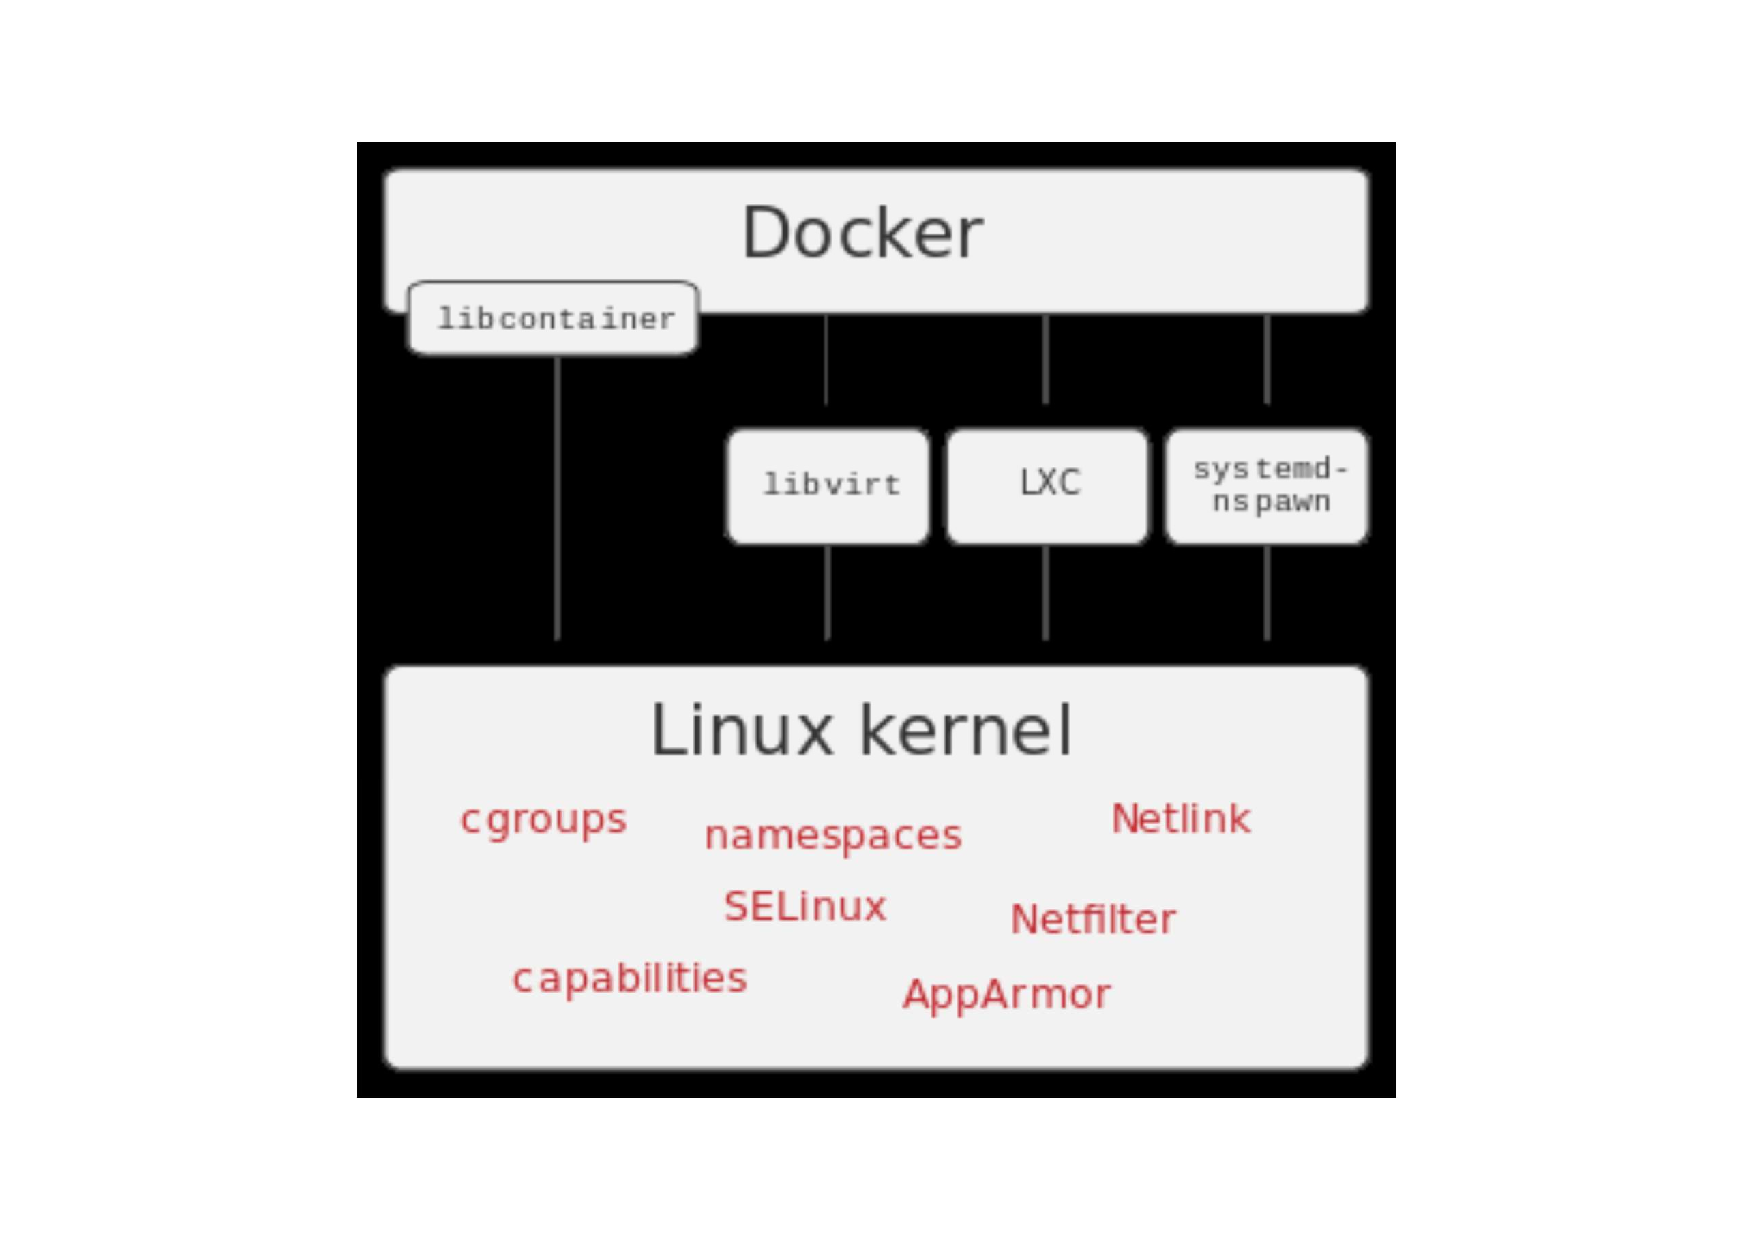
\includegraphics[width=\columnwidth]{Images/docker.pdf}  
	\caption[Docker Interfaces]{Docker can use different interfaces in order to access Linux kernel virtualization functionalities.}
	\label{fig:docker}
\end{figure}

\section{Symbolic Execution}
In computer science, the term symbolic execution refers to a software program analysis technique used to determine which data inputs cause the execution of each part of a program. It was introduced in the mid '70s~\cite{K-ICRS75,SELECT-ICRS75,K-CACM76,H-TSE77} mainly to test whether a software program could violate certain properties, e.g. that no divisions by zero are performed, no NULL pointers get dereferenced, no access to protected data can happen by unathorized users, etc. In general, it's not possible to decide every possible program property by means of automated checks, for example we cannot predict the target of an indirect jump. %, as it depends on values that are known at runtime. 
In practice, approximate and heuristic-based analyses are used in many cases, even in the field of mission-critical and security applications.

Software testing is performed to check that certain program properties hold for any possible usage scenario. A viable approach would be to test the program using a wide range of different, possibly random inputs. As the problem may occur only for very specific input values, we need to automate the exploration of the domain of the possible input data. 

With symbolic execution many possible execution paths are explored in parallel, without necessarily requiring concrete inputs. The idea is to replace the fully specified input data with symbols, that are their abstract representation, devolving to constraint solvers the construction of actual instances that would cause property violations. 

The symbolic execution intepreter walks through all the steps of the program, associating symbolic values to inputs rather than obtaining their actual values, building  expressions in terms of those symbols and program variables, and constraints in terms of the symbols corresponding to the possible outcomes of each conditional branch. 

When a program is run with a specific set of input data (a concrete execution), a single control flow path is explored. Hence, concrete executions can only under-approximate the analysis of the property of interest. With symbolic execution, multiple paths that a program could take under different inputs can be simultaneously explored. This means that a sound analyses can be done, giving stronger guarantees about the checked property~\cite{Baldoni:2018:SSE:3212709.3182657}. When a program runs with {\em symbolic} -- rather than concrete -- input values, the execution is performed by a {\em symbolic execution engine}, which builds and updates a structure to hold (i) a first-order Boolean {\em formula} describing the conditions satisfied by all the traversed branches along that path, and (ii) a {\em symbolic memory store} mapping variables to symbolic expressions or values, for each path traversed by the control flow. Execution of a branch updates the formula, while assignments update the symbolic store. Finally, a {\em model checker}, commonly based on a {\em satisfiability modulo theories} (SMT) solver~\cite{BKM14}, is  used to verify if the property is violated somewhere along each explored path and if the path itself is concretely feasible, i.e., if any assignment of concrete values to the program's symbolic arguments exists that satisfies its formula~\cite{Baldoni:2018:SSE:3212709.3182657}.

Symbolic execution techniques have been emphasized to a wide audience following the DARPA announcement in 2013 at the Cyber Grand Challenge, a two-year competition pursuing the creation of automatic systems for vulnerability detection, exploitation, and patching in near real-time~\cite{ANGR-SSP16}.
More important, symbolic execution based engines have been running 24/7 in the testing process of many Microsoft applications since 2008, discovering nearly 30\% of all the flaws discovered by file fuzz testing during the development of Windows 7, which other program analyses and blackbox testing techniques missed~\cite{SAGE-QUEUE12}.

\paragraph{An Introductory Example}


\label{symbolic-execution-example}
\begin{figure}[t]
	\begin{center}
		\begin{tabular}{c}
			\begin{lstlisting}[basicstyle=\ttfamily\scriptsize]
			1.  void foo(int a, int b) {
			2.     int x = 1, y = 0;
			3.     if (a != 0) {
			4.        y = 3+x;
			5.        if (b == 0)
			6.           x = 2*(a+b);
			7.     }
			8.     assert(x-y != 0);
			9.  }
			\end{lstlisting}
		\end{tabular}
	\end{center}
	\vspace{-2mm}
	\caption{Example: which values of \texttt{a} and \texttt{b} make the \texttt{assert} fail?}
	\label{fig:example-1}
	\vspace{-1.5mm}
\end{figure}

With reference to the C code in \MyFig{fig:example-1}, let's say we want to discover which of the $2^{32}$ possible \texttt{4-byte} inputs make the \texttt{assert} at line 8 of function \texttt{foo} fail. If we address the problem by running concretely the function \texttt{foo} on randomly generated inputs, we will unlikely pick up exactly the assert-failing inputs. Symbolic execution go beyond this limitation by reasoning on {\em classes of inputs}, rather than single input values, thanks to the evaluation of the code using symbols for its inputs, instead of concrete values,  

Going further into details, a symbol $\alpha_i$ is associated to each value that cannot be resolved by a static analysis of the code, e.g. an actual parameter of a function or data read from an input stream. At any time, the symbolic execution engine maintains a state $(stmt,~\sigma,~\pi)$ where:

\begin{itemize}
	\item $stmt$ is the next statement to evaluate. At this time being, we assume that $stmt$ can be an assignment, a conditional branch, or a jump.
	
	\item $\sigma$ is a {\em symbolic store} that associates program variables with either expressions over concrete values or symbolic values $\alpha_i$.
	
	\item $\pi$ denotes the {\em path constraints}, i.e., it is a formula expressing a set of assumptions on the symbols $\alpha_i$ as a result of branches taken in the execution to reach $stmt$. At the start of the analysis, $\pi=true$.
\end{itemize}

\noindent Depending on $stmt$, the symbolic engine changes the state as follows:

\begin{itemize}
	\item The evaluation of an assignment $x=e$ updates the symbolic store $\sigma$ by associating $x$ with a new symbolic expression $e_s$. We express this association with $x\mapsto e_s$, where $e_s$ is obtained by evaluating $e$ in the context of the current execution state and  can be any expression involving unary or binary operators over symbols and concrete values.
	\item The evaluation of a conditional branch ${\texttt if}~e~{\texttt then}~s_{true}~{\texttt else}~s_{false}$ affects the path constraints $\pi$. The symbolic execution is forked by creating two execution states with path constraints $\pi_{true}$ and $\pi_{false}$, respectively, which correspond to the two branches: $\pi_{true}=\pi \wedge e_s$ and $\pi_{false}=\pi \wedge \neg e_s$, where $e_s$ is a symbolic expression obtained by evaluating $e$. 
	Symbolic execution independently proceeds on both states.
	\item The evaluation of a jump {\texttt goto} $s$ updates the execution state by advancing the symbolic execution to statement $s$. 
\end{itemize}

\begin{figure}[t]
	\centering
	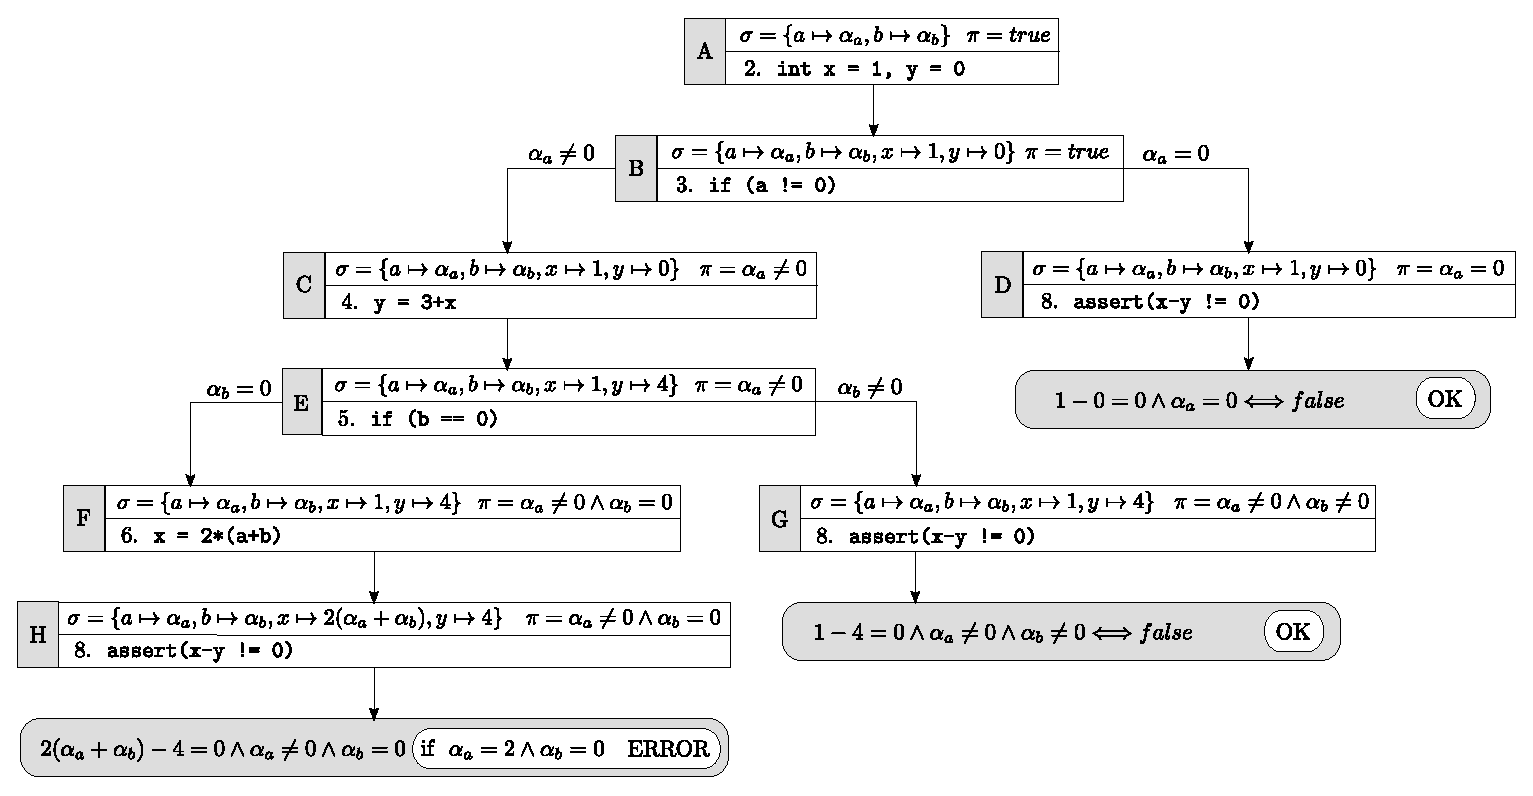
\includegraphics[width=0.975\columnwidth]{images/execution-tree.eps} 
	\caption{Symbolic execution tree of function {\texttt foo} given in \MyFig{fig:example-1}. Each execution state, labeled with an upper case letter, shows the statement to be executed, the symbolic store $\sigma$, and the path constraints $\pi$. Leaves are evaluated against the condition in the {\texttt assert} statement. }
	%For the sake of presentation the conjunction of constraints is shown as a list of constraints. }
	\label{fig:example-symbolic-execution}
	\vspace{-1mm}
\end{figure}

\noindent \MyFig{fig:example-symbolic-execution} shows a symbolic execution of function {\texttt foo}, that can be adequately represented as a tree. In the initial state (execution state $A$) the path constraints are {\texttt true} and input arguments {\texttt a} and {\texttt b} are associated with symbolic values. 
After local variables initialization {\texttt x} and {\texttt y} at line 2, the symbolic store is updated by associating {\texttt x} and {\texttt y} with concrete values 1 and 0, respectively (execution state $B$). A conditional branch is met in line 3 and the execution is forked:according to which branch is taken, a different statement is evaluated and different assumptions are made on symbol $\alpha_a$ (execution states $C$ and $D$). In the branch corresponding to $\alpha_a\neq 0$, variable {\texttt y} is assigned to  ${\texttt x}+3$, obtaining $y\mapsto 4$ in state $E$ because $x\mapsto 1$ in state $C$. Arithmetic expression evaluation, generally, change only the symbolic values.
When the {\texttt assert} at line 8 is reached by fully expanding every execution state  on all branches, we can check which input values for parameters {\texttt a} and {\texttt b} can make the {\texttt assert} fail. By analyzing execution states $\{D,G,H\}$, we can conclude that only $H$ can make {\texttt x-y = 0} true. The path constraints for $H$ at this point implicitly define the set of inputs that are unsafe for \texttt{foo}. 
In particular, any input values such that:
\[ 2(\alpha_a+\alpha_b)-4 = 0 \wedge \alpha_a \neq 0 \wedge \alpha_b = 0 \]
will make {\texttt assert} fail. An instance of unsafe input parameters can be eventually determined by invoking an {\em SMT solver}~\cite{BKM14} to solve the path constraints, which in this example would yield $a = 2$ and $b = 0$.

\subsubsection{Challenges of Symbolic Execution}
\label{example-discussion}

The example shown in Section~\ref{symbolic-execution-example} represents a case where symbolic execution can derive {\em all} the inputs that make the {\texttt assert} fail, by exploring all the possible execution states. With regards to the underpinning theory, exhaustive symbolic execution represents a {\em sound} and {\em complete} methodology for any decidable analysis. Soundness (no false negatives) means that all possible unsafe inputs are guaranteed to be found, while completeness (no false positives) means that  input values deemed unsafe are actually unsafe. Exhaustive symbolic execution cannot be easily scalable beyond small-sized applications. In many practical cases, a trade-off between soundness and performance approach is used.

Symbolic execution applied to real world applications faces many challenges, deriving from the increased complexity of those applications compared to the simplicity of our example. These challenges are pointed out by the following questions and observations:

\begin{itemize}
	\item \noindent {\em Pointers, arrays, or other complex objects}: how are they handled by the symbolic engine? Code manipulating pointers and data structures may identify memory addresses that are described by symbolic expressions, in addition to symbolic stored data.
	\item {\em Interactions across the software stack}: how are they handled by the engine? System code/library calls can have side effects, e.g. file creations, calls back to user code or callback functions that could affect the execution at a later stage of the computation and must be taken in account. 
	Evaluating all possible interaction outcomes may be unfeasible.
	\item {\em State space explosion}: how does symbolic execution deal with path explosion? The presence of iterative constructs in the language (iteration loops) can dramatically increase the number of execution states, up to the point where it becomes unfeasible for a symbolic execution engine to exhaustively explore all the possible states within a reasonable amount of time. 
	\item {\em Constraint solving}: what can a constraint solver do in practice?
	SMT solvers can scale to complex combinations of constraints over hundreds of variables. However, constructs such as non-linear arithmetic pose a major obstacle to efficiency.
	\item {\em Binary code}: what issues can arise when symbolically executing binary code?
	While our example of Section~\ref{symbolic-execution-example} is written in C, in many cases programs are only available as binary code. The availability of the source code of an application usually simplifies symbolic execution, as it can exploit high-level properties (e.g., object morphology) that can be inferred statically by analyzing the source code.
\end{itemize}
%Depending on the specific application context of symbolic execution

\noindent The above questions and assumptions are addressed in different ways and lead to different choices according to the specific contexts where symbolic execution is used. Typically these choices affect soundness or completeness, however this does not represent a serious limitation in many real cases where a partial exploration of the domain of possible execution states may provide enough information to reach the goal (e.g., determining which input values provokes an application failure) within specified time limits.

\subsection{Symbolic Execution Engines}
\label{se:executors}

In this section we describe some important principles for the design of symbolic executors and crucial tradeoffs that arise in their implementation. Moving from the concepts of concrete and symbolic runs, we also introduce the idea of {\em concolic} execution.

\subsubsection{Mixing Symbolic and Concrete Execution}
\label{ss:concrete-concolic-symbolic}

\begin{figure}[t]
	\centering
	%\vspace{-0.75mm}
	
\includegraphics[width=0.32\columnwidth]{images/concrete-abstract.eps} 
	\caption{Concrete and abstract execution machine models.}
	\label{fig:concrete-symbolic}
	\vspace{-1.5mm}
\end{figure}

As shown in the previous example, modeling all runs of concrete executions of real-world software programs is desirable but very often impossible in practice.

Symbolic execution, as we have described it so far, cannot explore feasible executions that would result in path constraints that cannot be dealt with~\cite{CS-CACM13}. Loss of soundness originates from many sources, e.g. untraceable external code, complex constraints involving non-linear arithmetic or transcendental functions. As constraint solving is a major performance barrier for an engine, we can assess the solvability in an absolute sense but also in terms of efficiency. Considering that practical programs are typically not self-contained, it is very challenging to statically analyze the whole software stack, especially considering the evaluation of every possible side effects.

One way to overcome this issue in practice is to mix concrete and symbolic execution, aka {\em concolic execution}, where the term concolic is a portmanteau of the words ``concrete'' and ``symbolic'' (Figure~\ref{fig:concrete-symbolic}). Some applications of this general principle are briefly discussed in the remainder of this section.


\newcommand{\dse}{DSE}
\paragraph{Dynamic Symbolic Execution} A common approach to concolic execution, known as {\em dynamic symbolic execution} (\dse) or {\em dynamic test  generation}~\cite{DART-PLDI05}, is to have concrete execution drive the symbolic one. A concrete store $\sigma_c$ is maintained, in addition to the symbolic and the path constraints stores, by the execution engine. It chooses an initial arbitrary input and executes the program both concretely and symbolically, by simultaneously updating the two stores and the path constraints. The symbolic execution wlaks through the same branch taken by the concrete execution, and the constraints extracted from the branch condition are added to the current set of path constraints. The symbolic engine does not need to invoke the constraint solver to decide if a branch condition is satisfiable, as this is already tested by the concrete execution. Since not all the paths might be explored by concrete execution, the path conditions associated to a branch can be negated and passed to the SMT solver to determine a satisfying assignment for the new constraints, i.e., to generate a new input. This strategy can be repeated until the desired path coverage is reached.

\vspace{-2pt} 
%\boxedexample{
\fbox{
\begin{minipage}{4.3 in}
	Consider the C function in Figure~\ref{fig:example-1} and suppose to choose $a = 1$ and $b = 1$ as input parameters. Under these conditions, the concrete execution takes path $A\leadsto B\leadsto C\leadsto E\leadsto G$ in the symbolic tree of Figure~\ref{fig:example-symbolic-execution}. Besides the symbolic stores shown in Figure~\ref{fig:example-symbolic-execution}, the concrete stores maintained in the traversed states are the following:
	\begin{enumerate}
		
		\item[]$-$~~$\sigma_c=\{a\mapsto 1,~b\mapsto 1\}$ in state $A$;
		\item[]$-$~~$\sigma_c=\{a\mapsto 1,~b\mapsto 1,~x\mapsto 1,~y\mapsto 0\}$ in states $B$ and $C$;
		\item[]$-$~~$\sigma_c=\{a\mapsto 1,~b\mapsto 1,~x\mapsto 1,~y\mapsto 4\}$ in states $E$ and $G$.
		
	\end{enumerate}  
	%Stores and path constraints maintained by the concolic run are shown in Figure~\ref{fig:example-concolic-execution}. 
	After checking that the \texttt{assert} conditions at line 8 succeed, we can generate a new control flow path by negating the last path constraint, i.e., $\alpha_b\neq 0$. The solver at this point would generate a new input that satisfies the constraints $\alpha_a\neq 0\,\wedge\, \alpha_b=0$ (for instance $a = 1$ and $b = 0$) and the execution would continue in a similar way along the path $A\leadsto B\leadsto C\leadsto E\leadsto F$. %
\end{minipage}}

\vspace{+10pt}
Although \dse\ uses concrete inputs to drive the symbolic execution toward a specific path, it still needs to pick a branch to negate whenever a new path has to be explored. Notice also that each concrete execution may add new branches that will have to be visited. Since the set of non-taken branches across all performed concrete executions can be very large, adopting effective search heuristics (Section~\ref{ss:heuristics}) can play a crucial role. For instance, {\textsc DART}~\cite{DART-PLDI05} chooses the next branch to negate using a depth-first strategy. Additional strategies for picking the next branch to negate have been presented in literature. For instance, the {\em generational search} of {\textsc SAGE}~\cite{SAGE-NDSS08} systematically yet partially explores the state space, maximizing the number of new tests generated while also avoiding redundancies in the search. This is achieved by negating constraints following a specific order and by limiting the backtracking of the search algorithm. Since the state space is only partially explored, the initial input plays a crucial role in the effectiveness of the overall approach.  The importance of the first input is similar to what happens in traditional {\em black-box fuzzing}; hence, symbolic engines such as {\textsc SAGE} are often referred to as {\em white-box fuzzers}.

The symbolic information maintained during a concrete run can be exploited by the engine to obtain new inputs and explore new paths. The next example shows how DSE can handle invocations to external code that is not symbolically tracked by the concolic engine.



\vspace{10pt}
%\boxedexample{
\fbox{
	\begin{minipage}{4.3 in}
	Consider function {\texttt foo} in Figure~\ref{fig:example-concolic-problems}a and suppose that {\texttt bar} is not symbolically tracked by the concolic engine (e.g., it could be provided by a third-party component, written in a different language, or analyzed following a black-box approach). Assuming that $x = 1$ and $y = 2$ are randomly chosen as the initial input parameters, the concolic engine executes {\texttt bar} (which returns $a = 0$) and skips the branch that would trigger the error statement. At the same time, the symbolic execution tracks the path constraint $\alpha_y \geq 0$ inside function {\texttt foo}. Notice that branch conditions in function {\texttt bar} are not known to the engine. To explore the alternative path, the engine negates the path constraint of the branch in {\texttt foo}, generating inputs, such as $x = 1$ and $y = -4$, that actually drive the concrete execution to the alternative path. With this approach, the engine can explore both paths in {\texttt foo} even if {\texttt bar} is not symbolically tracked. 
	
	A variant of the previous code is shown in Figure~\ref{fig:example-concolic-problems}b, where function {\texttt qux} -- differently from {\texttt foo} -- takes a single input parameter but checks the result of {\texttt bar} in the branch condition. Although the engine can track the path constraint in the branch condition tested inside {\texttt qux}, there is no guarantee that an input able to drive the execution toward the alternative path is generated: the relationship between $a$ and $x$ is not known to the concolic engine, as {\texttt bar} is not symbolically tracked. In this case, the engine could re-run the code using a different random input, but in the end it could fail to explore one interesting path in {\texttt qux}. 
	
	A related issue is presented by Figure~\ref{fig:example-concolic-problems}c. We observe a {\em path divergence} when inputs generated for a predicted path lead execution to a different path. In general, this can be due to symbol propagation not being tracked, resulting in inaccurate path constraints, or to imprecision in modeling certain (e.g., bitwise, floating-point) operations in the engine. In the example, function {\texttt baz} invokes the external function {\texttt abs}, which performs a side effect on $x$ by assigning it with its absolute value. Choosing $x = 1$ as the initial concrete value, the concrete execution does not trigger the error statement, but the concolic engine tracks the path constraint $\alpha_x \geq 0$ due to the branch in {\texttt baz}, trying to generate a new input by negating it. However the new input, e.g., $x = -1$, does not trigger the error statement due to the (untracked) side effects of {\texttt abs}. Interestingly, the engine has no way of detecting that no input can actually trigger the error.
	% {\texttt abs}, which simply computes the absolute value of a number
	%In this case, after generating a new input the engine detects a {\em path divergence}: a concrete execution that does not follow the predicted path. Interestingly, in this example no input could actually trigger the error, but the engine is not able to detect this property.
\end{minipage}}

\begin{figure*}[t]
	\vspace{-2.5mm}
	%\centering
	\begin{minipage}{.30\textwidth}
		\begin{lstlisting}[basicstyle=\ttfamily\scriptsize]
void foo(int x, int y) {
int a = bar(x);
if (y < 0) ERROR;
} 
		\end{lstlisting}
		%int bar(int z) {
		%   if (z == 23) return 1;
		%   return 0;
		%}
		\vspace{-4mm}
		%\caption{}
	\end{minipage}%
	%
	\hspace{5mm}
	%
	\begin{minipage}{.30\textwidth}
		%\vspace{5mm}
		\begin{lstlisting}[basicstyle=\ttfamily\scriptsize]
void qux(int x) {
int a = bar(x);
if (a > 0) ERROR;
} 
		\end{lstlisting}
		%int bar(int z) {
		%   if (z == 23) return 1;
		%   return 0;
		%}
		\vspace{-4mm}
		%\caption{}
	\end{minipage}%
	%
	\hspace{5mm}
	%
	\begin{minipage}{.30\textwidth}
		%\vspace{5mm}
		\begin{lstlisting}[basicstyle=\ttfamily\scriptsize]
void baz(int x) {
abs(&x);
if (x < 0) ERROR;
}   
		\end{lstlisting}
		%void abs(int * z) {
		%   if (*z < 0) *z = -(*z);
		%}
		\vspace{-4mm}
		%\caption{}
	\end{minipage}%
\begin{Verbatim}[obeytabs]
	a)		     b)			c)
\end{Verbatim}
	\vspace{+2pt}
	\caption{Concolic execution: (a) testing of function {\texttt foo} even when {\texttt bar} cannot be symbolically tracked by an engine, (b) example of false negative, and (c) example of a path divergence, where \texttt{abs} drops the sign of the integer at \texttt{\&x}.
		%(b) Example of a missed path: assuming that function {\tt bar} is not symbolically tracked, then it is unlikely that the engine will be able to generate an input that trigger execution of function {\tt error} inside function {\tt qux}. (c) Example of a path divergence: assuming that function {\tt abs} is not tracked, then the concolic engine may try to generate fruitlessly an input able to trigger execution of function {\tt error} in function {\tt baz}.
	}
	\label{fig:example-concolic-problems}
	\vspace{-3mm}
\end{figure*}




As shown by the example, false negatives (i.e., missed paths) and path divergences are notable downsides of dynamic symbolic execution. \dse\ trades soundness for performance and implementation effort: false negatives are possible, because some program executions -- and therefore possible erroneous behaviors -- may be missed, leading to a {\em complete}, but {\em under-approximate} form of program analysis. Path divergences have been frequently observed in literature: for instance,~\cite{SAGE-NDSS08} reports rates over $60\%$. \cite{CLH-SCN15} presents an empirical study of path divergences, analyzing the main patterns that contribute to this phenomenon. External calls, exceptions, type casts, and symbolic pointers are pinpointed as critical aspects of concolic execution that must be carefully handled by an engine to reduce the number of path divergences.

\paragraph{Selective Symbolic Execution}
{\textsc \stwoe}~\cite{CKC-TOCS12} takes a different approach to mix symbolic and concrete execution based on the observation that one might want to explore only some components of a software stack in full, not caring about others. {\em Selective symbolic execution} carefully interleaves concrete and symbolic execution, while keeping the overall exploration meaningful.
%{\em Selective symbolic execution} carefully interleaves concrete executions of functions with fully symbolic phases, while keeping the exploration meaningful.

Suppose a function A calls a function B and the execution mode changes at the call site. Two scenarios arise:
(1) {\em From concrete to symbolic and back}: the arguments of B are made symbolic and B is explored symbolically in full. B is also executed concretely and its concrete result is returned to A. After that, A resumes concretely. 
(2) {\em From symbolic to concrete and back}: the arguments of B are concretized, B is executed concretely, and execution resumes symbolically in A. This may impact both soundness and completeness of the analysis: (i) {\em Completeness}: to make sure that symbolic execution skips any paths that would not be realizable due to the performed concretization (possibly leading to false positives), {\textsc \stwoe} collects path constraints that keep track of how arguments are concretized, what side effects are made by B, and what return value it produces. (ii) {\em Soundness}: concretization may cause missed branches after A is resumed (possibly leading to false negatives). To remedy this, the collected constraints are marked as {\em soft}: whenever a branch after returning to A is made inoperative by a soft constraint, the execution backtracks and a different choice of arguments for B is attempted. To guide re-concretization of B's arguments, {\textsc \stwoe} also collects the branch conditions during the concrete execution of B, and chooses the concrete values so that they enable a different concrete execution path in B.

%===================================================================================
\subsection{Path Selection}
\label{ss:heuristics}

Since enumerating all paths of a program can be prohibitively expensive, in many software engineering activities related to testing and debugging the search is prioritized by looking at the most promising paths first. Among several strategies for selecting the next path to be explored, we now briefly overview some of the most effective ones. %in prior works.
%
We remark that path selection heuristics are often tailored to help the symbolic engine achieve specific goals (e.g., overflow detection). Finding a universally optimal strategy remains an open problem.

{\em Depth-first search} (DFS), which expands a path as much as possible before backtracking to the deepest unexplored branch, and {\em breadth-first search} (BFS), which expands all paths in parallel, are the most common strategies. DFS is often adopted when memory usage is at a premium, but is hampered by paths containing loops and recursive calls. Hence,  in spite of the higher memory pressure and of the long time required to complete the exploration of specific paths, some tools resort to BFS, which allows the engine to quickly explore diverse paths  detecting interesting behaviors early.
%\iffullver{On the other hand, if the ultimate goal requires to fully terminate the exploration of one or more paths, BFS may take a very long time}{}
Another popular strategy is {\em random path selection}, that has been refined in several variants. For instance, {\textsc KLEE}~\cite{KLEE-OSDI08} assigns probabilities to paths based on their length and on the branch arity: it favors paths that have been explored fewer times, preventing starvation caused by loops and other path explosion factors.

% have instead presented
Several works, such as {\textsc EXE}~\cite{EXE-CCS06}, {\textsc KLEE}~\cite{KLEE-OSDI08}, {\textsc Mayhem}~\cite{MAYHEM-SP12}, and {\textsc \stwoe}~\cite{CKC-TOCS12}, have discussed heuristics aimed at maximizing code coverage. For instance, the {\em coverage optimize search} discussed in {\textsc KLEE}~\cite{KLEE-OSDI08} computes for each state a weight, which is later used to randomly select states. The weight is obtained by considering how far the nearest uncovered instruction is, whether new code was recently covered by the state, and the state's call stack. Of a similar flavor is the heuristic proposed in~\cite{LZL-OOPSLA13}, called {\em subpath-guided search}, which attempts to explore {\textit less traveled} parts of a program by selecting the subpath of the control flow graph that has been explored fewer times. This is achieved by maintaining a frequency distribution of explored subpaths, where a subpath is defined as a consecutive subsequence of length $n$ from a complete path. Interestingly, the value $n$ plays a crucial role with respect to the code coverage achieved by a symbolic engine using this heuristic and no specific value has been shown to be universally optimal. %
%Another interesting search strategy is the {\em shortest-distance symbolic execution} heuristic presented in~\cite{MPF-SAS11}. The work does not target coverage, but aims at identifying program inputs that trigger the execution of a specific point in a program. However, similarly to coverage-based strategies, it is based on a metric for evaluating the shortest distance to the target point. This is computed as the length of the shortest path in the inter-procedural control-flow graph, and paths with the shortest distance are prioritized by the engine. 
{\em Shortest-distance symbolic execution}~\cite{MPF-SAS11} does not target coverage, but aims at identifying program inputs that trigger the execution of a specific point in a program. The heuristic is based however, as in coverage-based strategies, on a metric for evaluating the shortest distance to the target point. This is computed as the length of the shortest path in the inter-procedural control flow graph, and paths with the shortest distance are prioritized by the engine. 

%Other search heuristics try to prioritize paths likely leading to states that are {\em interesting} according to some goal. For instance, the {\em buggy-path first} strategy in {\textsc AEG}~\cite{AEG-NDSS11} picks paths whose past states have contained small but unexploitable bugs. The intuition is that if a path contains some small errors, it is likely that it has not been properly tested. There is thus a good chance that future states may contain interesting, and hopefully exploitable, bugs. Similarly, the {\em loop exhaustion} strategy discussed in {\textsc AEG}~\cite{AEG-NDSS11} explores paths that visit loops. This approach is inspired by the practical observation that common programming mistakes in loops may lead to buffer overflows or other memory-related errors. In order to find exploitable bugs, {\textsc Mayhem}~\cite{MAYHEM-SP12} instead gives priority to paths where symbolic memory accesses are identified or symbolic instruction pointers are detected. 

Other search heuristics try to prioritize paths likely leading to states that are {\em interesting} according to some goal. For instance, {\textsc AEG}~\cite{AEG-NDSS11} introduces two such strategies. The {\em buggy-path first} strategy picks paths whose past states have contained small but unexploitable bugs. The intuition is that if a path contains some small errors, it is likely that it has not been properly tested. There is thus a good chance that future states may contain interesting, and hopefully exploitable, bugs. Similarly, the {\em loop exhaustion} strategy explores paths that visit loops. This approach is inspired by the practical observation that common programming mistakes in loops may lead to buffer overflows or other memory-related errors. In order to find exploitable bugs, {\textsc Mayhem}~\cite{MAYHEM-SP12} instead gives priority to paths where memory accesses to symbolic addresses are identified or symbolic instruction pointers are detected. 

\cite{ZCWDL15} proposes a novel method of dynamic symbolic execution to automatically find a program path satisfying a regular property, i.e., a property (such as file usage or memory safety) that can be represented by a Finite State Machine (FSM). Dynamic symbolic execution is guided by the FSM so that branches of an execution path that are most likely to satisfy the property are explored first. The approach exploits both static and dynamic analysis to compute the priority of a path to be selected for exploration: the states of the FSM that the current execution path has already reached are computed dynamically during the symbolic execution, while backward data-flow analysis is used to compute the future states statically. If the intersection of these two sets is non-empty, there is likely a path satisfying the property.

{\em Fitness functions} have been largely used in the context of search-based test generation~\cite{M-STVR04}. %\mynote{[D] Check and rephrase 2nd sentence}
A fitness function measures how close an explored path is to achieve the target test coverage. Several works, e.g.,~\cite{XTD-DSN09,CS-CACM13}, have applied this idea in the context of symbolic execution. As an example,~\cite{XTD-DSN09} introduces {\em fitnex}, a strategy for flipping branches in concolic execution that prioritizes paths likely {\em closer} to take a specific branch.
In more detail, given a target branch with an associated condition of the form $|a - c| == 0$, the closeness of a path is computed as $|a - c|$ by leveraging the concrete values of variables $a$ and $c$ in that path. Similar fitness values can be computed for other kinds of branch conditions. The path with the lowest fitness value for a branch is selected by the symbolic engine. Paths that have not reached the branch yet get the worst-case fitness value. 

%In more detail, given a branch condition of the form $|a - c| == 0$ and a \mynote{I: l'inglese (e il concetto) non e' molto chiaro, si puo' spiegare meglio?}  path that has reached the branch, {\em fitnex} computes a closeness equal to $|a - c|$ by leveraging the concrete values \iffullver{of the two}{of} variables $a$ and $c$ in that path. Similar fitness values can be computed for other kinds of branch conditions. The path with the lowest fitness value for a branch is selected by the symbolic engine. Paths that have not reached the branch yet get the worst-case fitness value. 

% \mytempedit{
% Different works~\cite{DA-ASE14,MPF-SAS11} aim at identifying program inputs that trigger the execution of a specific target point in a program.
% %: this goal is often referred as the {\em line reachability problem}. 
% For instance,~\cite{MPF-SAS11} presents different strategies to achieve this goal. Similarly to coverage-based heuristics, the {\em shortest-distance symbolic execution} strategy (SDSE) exploits a metric for evaluating the shortest distance to a target point (instead of any uncovered line in the code). This metric is defined as the length of the shortest path in the inter-procedural control-flow graph (ICFG). Paths with the shortest distance are prioritized by the engine. 
% %
% On the other hand, the {\em call-chain backward symbolic execution} strategy (CCBSE) works very differently. It starts by determining a valid path in the function where the target line is located. When a path is found, the strategy backwards to one of the possible callers of the function that contains the target point and tries to reconstruct a valid path from the entry point of the caller to the target point. This process is recursively repeated until a valid path from the main function of the program has been reconstructed. The main difference with respect to symbolic backward execution (see Section~\ref{se:executors}) is that, although CCBSE follows the call-chain backwards from the target point, inside each function the exploration is done as in traditional forward symbolic execution. Since both SDSE and CCBSE can behave poorly in some specific cases,~\cite{MPF-SAS11} has also proposed {\em Mix-CCBSE}, a combination of these two strategies that can perform very effectively in practice.
% }


%===================================================================================
%\subsubsection{Caching} 
%\label{ss:caching}

%Caching is a powerful technique to achieve time-space tradeoffs and is embodied in symbolic executors in different ways. Most prominently:

%\begin{itemize}[topsep=3pt] % TODO

%\item {\em Function caching.} A function $f$, and more in general any part of a program, may be called multiple times during an execution, either at the same calling context or at different ones. The traditional symbolic execution approach requires to symbolically execute $f$ at each call. \cite{G-POPL07} proposes a compositional approach that dynamically generates {\em function summaries}, allowing the symbolic executor to effectively reuse prior discovered analysis results. A similar idea has been also proposed in~\cite{BCE-TACAS08}. The main intuition is that, if two program states differ only for some program values that are not read later, the executions generated by the two program states will produce the same side effects. Side effects of a portion of code can be therefore cached and possibly reused later. 

%Since the two techniques are almost equivalent, our discussion will follow~\cite{G-POPL07}. 
%\paragraph{Definition of function summaries} A function summary $\phi_f$ for a function $f$ is defined as a propositional logic formula. It can be computed by successive iterations and defined as a disjunction of formulas $\phi_w$ of the form $\phi_w = {pre}_w \wedge post_w$, where $w$ is a possible execution path of function $f$, $pre_w$ is a conjunction of constraints over the inputs of $f$, and $post_w$ is a conjunction of constraints over the outputs of $f$. Formally, $\phi_f = \bigvee \phi_w$.  
%
%\paragraph{Using function summaries} Whenever a function $f$ is called, the symbolic execution engine checks whether a summary $\phi_w$ of $f$ with $pre_w$ compliant with the current path constraints is available. If so, the post conditions $post_w$ are added to the current symbolic state. Otherwise, if no matching summary is found, a new function summary is computed.
%
%\paragraph{Computing function summaries} Function summaries can be computed dynamically: whenever there is an invocation of a function $f$, $pre_w$ is obtained from the current set of constraints over the input of $f$, while $post_w$ is given by tracking constraints over the \mynote{[D] no symbolic?}concolic\footnote{{\em [D] If this technique applies to concolic executors only we should say it upfront!}} execution of function $f$ over some concrete inputs that are compliant with $pre_w$. Notice that $pre_w$ defines an equivalence class of concrete executions that result in executions characterized by $post_w$. 
%
%\paragraph{Issues} If the symbolic execution engine cannot reason on one or more statements contained in a function $f$, then the generated summary cannot be \mynote{[D] blindly}blindly reused. For instance, consider a function that contains a call to an external function (e.g., a system call) or to a {\em complex} one (e.g., a hash function). In this scenario, even if a matching function summary is found, the related post conditions $post_w$ may not be valid since they have been generated over a concrete execution and thus cannot be generalized. % robust hash function

%\item {\em Loop summarization.} In order to avoid redundant executions of the same loop under the same program state, loop summaries can be computed and cached for later reuse, similarly to function summaries. We refer to Section~\ref{se:loops} for details on a loop summarization strategy proposed in~\cite{GL-ISSTA11}.

%\item {\em Constraint reuse.} In order to speed up constraint solving, different works support the reuse of constraint solutions based on semantic or syntactic equivalence of the constraints. Examples are given in {\textsc EXE}~\cite{EXE-CCS06}, {\textsc KLEE}~\cite{KLEE-OSDI08}, and~\cite{MEMO-ISSTA12,GREEN-FSE12}. We will further discuss this optimization in Section~\ref{se:constraint-solving}.

%\end{itemize}

%\vspace{-1mm}

\subsection{Symbolic Backward Execution}
\label{ss:backward}
% Symbolic backward execution (SBE)~\cite{CFS-PLDI09,DA-ASE14} is a variant of symbolic execution that proceeds its exploration backward from a target point of a program to an entry point of a program. In other words, the analysis is performed in the reversed direction with respect to a traditional (forward) symbolic execution.
Symbolic backward execution (SBE)~\cite{CFS-PLDI09,DA-ASE14} is a variant of symbolic execution in which the exploration proceeds from a target point to an entry point of a program. The analysis is thus performed in the reverse direction than in canonical (forward) symbolic execution. The main purpose of this approach is typically to identify a test input instance that can trigger the execution of a specific line of code (e.g., an {\texttt assert} or {\texttt throw} statement). %  
This can be very useful for a developer when performing debugging or regression testing over a program.
As the exploration starts from the target, path constraints are collected along the branches met during the traversal. Multiple paths can be explored at a time by an SBE engine and, akin to forward symbolic execution, paths are periodically checked for feasibility. When a path condition is proved unsatisfiable, the engine discards the path and backtracks.
%SBE starts its exploration from a target point and steps backwards into the code, collecting the path constraints given by the branches that are met during the traversal. In general, multiple paths can be simultaneously explored by a SBE engine. Akin to forward symbolic execution, paths are periodically checked to verify their feasibility. Whenever a path condition is proven to be unsatisfiable, the engine discards the path and then backtracks. 


\cite{MPF-SAS11} discusses a variant of SBE dubbed {\em call-chain backward symbolic execution}~(CCBSE). The technique starts by determining a valid path in the function where the target line is located. When a path is found, the engine moves to one of the callers of the function that contains the target point and tries to reconstruct a valid path from the entry point of the caller to the target point. The process is recursively repeated until a valid path from the main function of the program has been reconstructed. The main difference with respect to the traditional SBE is that, although CCBSE follows the call-chain backwards from the target point, inside each function the exploration is done as in traditional symbolic execution.

%A variant of SBE has been discussed by~\cite{MPF-SAS11} with the {\em call-chain backward symbolic execution} strategy (CCBSE). This technique starts by determining a valid path in the function where the target line is located. When a path is found, the strategy backwards to one of the callers of the function that contains the target point and tries to reconstruct a valid path from the entry point of the caller to the target point. This process is recursively repeated until a valid path from the main function of the program has been reconstructed. The main difference with respect to the traditional SBE is that, although CCBSE follows the call-chain backwards from the target point, inside each function the exploration is done as in traditional symbolic execution.

% TODO
% \iffullver{ (see, e.g., the discussion about CFG reconstruction in Section~\ref{se:symbolic-binary}).}{\mynote{cite appendix or some paper?}.} 
A crucial requirement for the reversed exploration in SBE, as well as in CCBSE, is the availability of the inter-procedural control flow graph which provides a whole-program control flow and makes it possible to determine the call sites for the functions that are involved in the exploration. Unfortunately, constructing such a graph can be quite challenging in practice. Moreover, a function may have many possible call sites, making the exploration performed by a SBE still very expensive. On the other hand, some practical advantages can arise when the constraints are collected in the reverse direction.


%===================================================================================
\vspace{-2mm}
\subsection{Design Principles of Symbolic Executors}
\label{ss:principles}

A number %\mynote{[D] why MAYHEM?}  
of performance-related design principles that a symbolic execution engine should follow are  summarized in %{\textsc Mayhem}
\cite{MAYHEM-SP12}. Most notably:
\begin{enumerate}
	\item {\em Progress}: the executor should be able to proceed for an arbitrarily long time without exceeding the given resources. Memory consumption can be especially critical, due to the potentially gargantuan number of distinct control flow paths.
	\item {\em Work repetition}: no execution work should be repeated, avoiding to restart a program several times from its very beginning in order to analyze different paths that might have a  common prefix.
	\item {\em Analysis reuse}: analysis results from previous runs should be reused as much as possible. In particular, costly invocations to the SMT solver on  previously solved path constraints should be avoided.
\end{enumerate}

\noindent Due to the large size of the execution state space to be analyzed, different symbolic engines have explored different trade-offs between, e.g., running time and memory consumption, or performance and soundness/completeness of the analysis.

Symbolic executors that attempt to execute multiple paths simultaneously in a single run -- also called {\em online} -- clone the execution state at each input-dependent branch. Examples are given in {\textsc KLEE}~\cite{KLEE-OSDI08}, {\textsc AEG}~\cite{AEG-NDSS11}, {\textsc \stwoe}~\cite{CKC-TOCS12}. These engines never re-execute previous instructions, thus avoiding work repetition. However, many active states need to be kept in memory and memory consumption can be large, possibly hindering progress. Effective techniques for reducing the memory footprint include {\em copy-on-write}, which tries to share as much as possible between different states~\cite{KLEE-OSDI08}. As another issue, executing multiple paths in parallel requires to ensure isolation between execution states, e.g., keeping different states of the OS by emulating the effects of system calls.

Reasoning about a single path at a time, as in concolic execution, is the approach taken by so-called {\em offline executors}, such as {\textsc SAGE}~\cite{SAGE-NDSS08}. Running each path independently of the others results in low memory consumption with respect to online executors and in the capability of reusing immediately analysis results from previous runs. On the other side, work can be largely repeated, since each run usually restarts the execution of the program from the very beginning. In a typical implementation of offline executors, runs are concrete and require an input seed: the program is first executed concretely, a trace of instructions is recorded, and the recorded trace is then executed symbolically.
%
{\em Hybrid executors} such as {\textsc Mayhem}~\cite{MAYHEM-SP12} attempt at balancing between speed and memory requirements: they start in online mode and generate checkpoints, rather than forking new executors, when memory usage or the number of concurrently active states reaches a threshold. Checkpoints maintain the symbolic execution state and replay information. When a checkpoint is picked for restoration, online exploration is resumed from a restored concrete state.
%: mixed approach. Start with an online approach, if needed switch to offline mode by doing checkpoints. A checkpoint contains the symbolic execution state and replay information. Concrete execution state is discarded since it can be quickly recovered at runtime by using one input generated by the solver before checkpointing. 
	\chapter{xSpark} \label{chap:xSpark}
%\begin{flushright}{\slshape    
%   Science, my boy, is made up of mistakes, but they are mistakes
%   which it is useful to make, because they lead little by little
%   to the truth}. \\ \medskip --- \citeauthor{verne_journey:1957}
%   \citetitle{verne_journey:1957} \citeyear{verne_journey:1957}
%\end{flushright} 
\lettrine[lines=4]{\textcolor{purple}{T}}{his} chapter illustrates the previous works done on xSpark, that is the base for the developments made and contribution given by this thesis.
%\section{xSpark}\label{sec:xSpark}
xSpark is a Spark extension that offers optimized and elastic provisioning of resources in order to meet execution deadlines. This is obtained by using nested control loops. A centralized control loop, implemented on the master node, controls the execution of the different stages of an application; at the same time multiple local loops, one per
executor, focus on task execution.
\begin{figure}
	\centering
	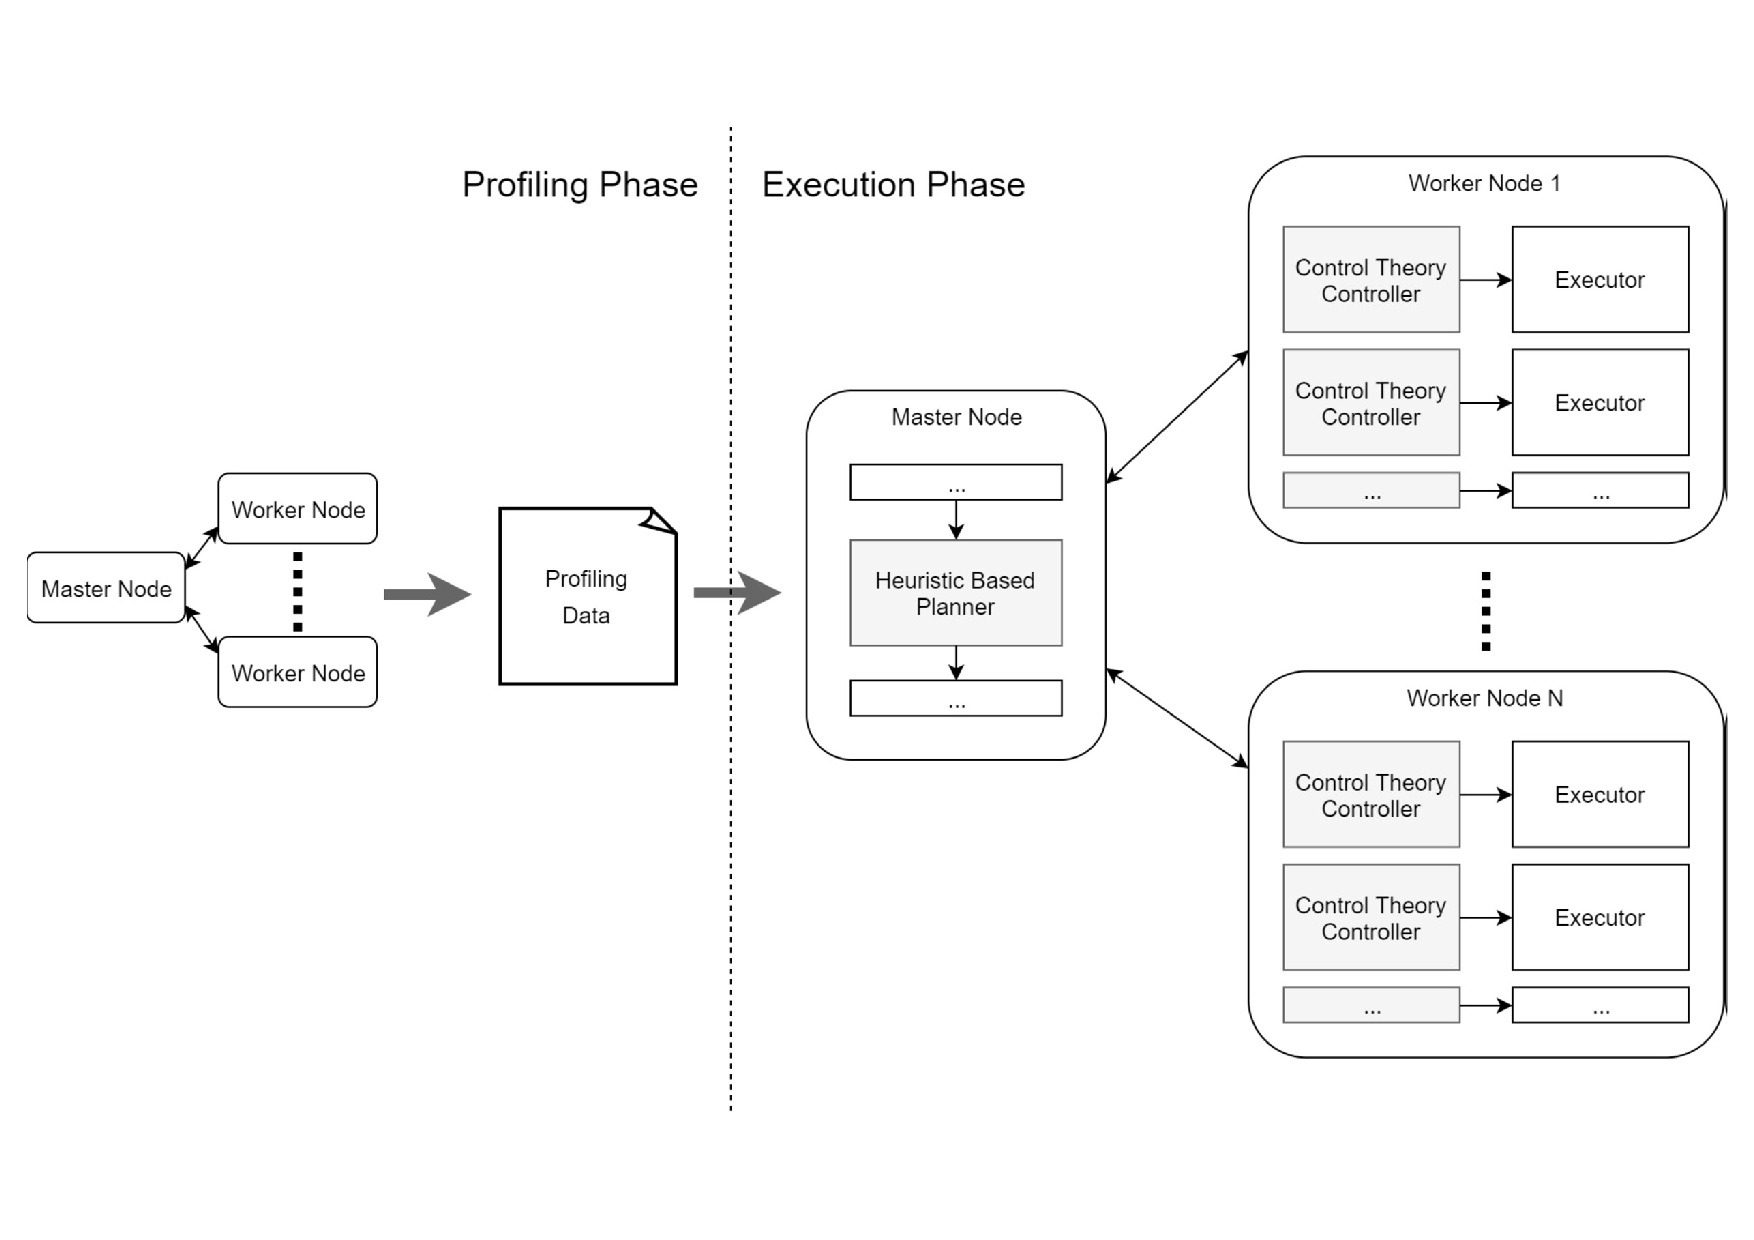
\includegraphics[width=\columnwidth]{Images/xspark_execution_flow.pdf}  
	\caption[xSpark high level setup and execution flow]{High level setup and execution flow of xSpark.}
	\label{fig:xSparkExecFlow}
\end{figure}

In \MyFig{fig:xSparkExecFlow} we can see a high level representation of xSpark execution flow. A preliminary Profiling Phase, that is executed once per application, is obtained by executing the application once to obtain information about its runtime execution. The log generated by the application are used to generate its Profiling Data.

In the Execution Phase, we control the application by means of xSpark’s control loops. 
The centralized control loop is represented as a Heuristic Based Planner, which exploits the profiling data, that are used to understand the amount of work that is needed to execute the application. This component uses the provided profiling data to determine the amount of resources to assign to executors for each of the application stages, in order to complete the execution within the given deadline. The local loops instead are represented as control theory controllers. They perform fine-grained tuning of the resources assigned to each of the executors using a control theory based controller. This component is used to counteract the possible imprecision of the estimated needed resources, which may be caused by different factors, such as the available memory, etc.

Usually Spark applications are run multiple times, as they are reusable and long lasting assets. xSpark exploits an initial profiling phase to create an enriched \textit{Directed Acyclic Graph} (DAG) ot \textit{Parallel Execution Plan} (\plan) describing the entire application execution flow, by collecting information about all the stages of the application. For each stage, xSpark annotates the DAG with the execution time (stage duration), the number of task processed, the number of input records read, the number of output record written and the nominal rate, defined as the number of records that a single core processes during one second of execution. 

%\lstinputlisting[
%firstline=1,
%lastline=19,
%float=tb,
%language=Python,
%tabsize=2,
%numbers=left,
%numberstyle=\tiny,
%stepnumber=1,
%numbersep=5pt,
%caption={Example of profiling data from a PageRank application.}, 
%captionpos=t,
%label=lst:profileFragment
%]{CodeFiles/profileFragment.json}

\begin{figure}
	\centering
	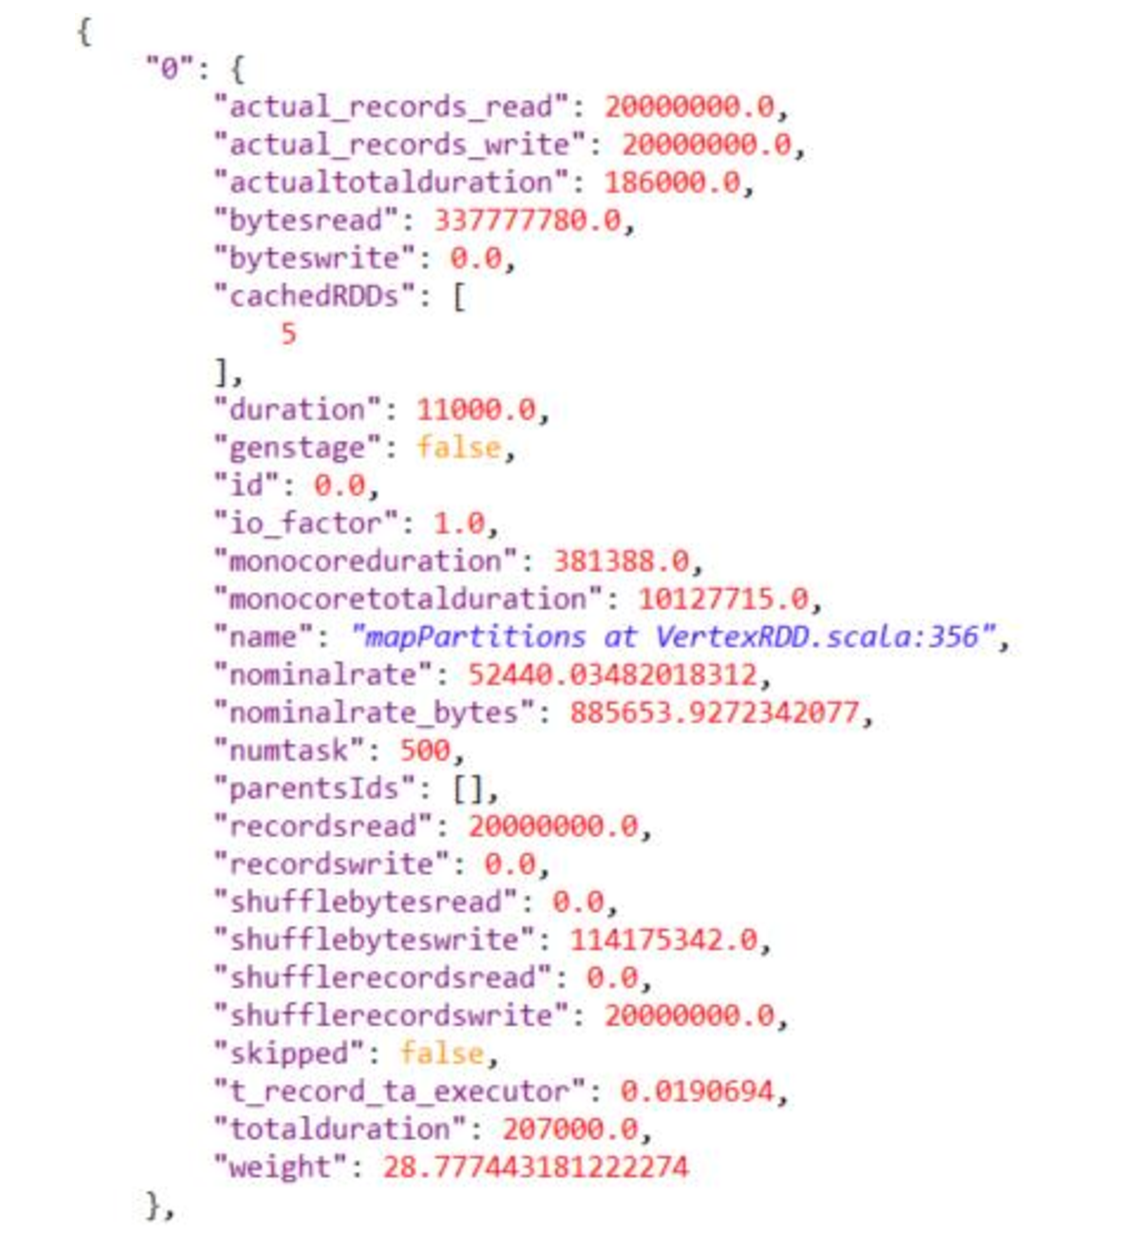
\includegraphics[width=\columnwidth]{Images/profile_fragment.pdf}  
	\caption[Example of profiling data from a Louvain application]{Example of profiling data from a Louvain application.}
	\label{fig:profileFragment}
\end{figure}

%In \MyListing{lst:profileFragment}
In \MyFig{fig:profileFragment} we can see a fragment, relative to stage number zero, of the profiling data of a Louvain application executed in xSpark.
The duration field contains the serialized total duration of the tasks in milliseconds.

At runtime, the a\plan allows the xSpark scheduler function to know how much
work was already completed and how much remains to be done. This means that xSpark can only optimize the allocation of the resources if all the executions of the same application use the same \plan. This might not always be the case, for example when the code contains branches or loops, because these might need to be resolved in different ways at runtime. If the application \plan at runtime differs from the one obtained during the profiling phase, xSpark is not able to estimate the amount of remaining work. 

The centralized control loop is activated before the execution of every stage, it uses a heuristic, explained in \MySec{sec:heuristic}, in order to assign a deadline to the stage, calculate the amount of CPU cores that are needed to satisfy it, and assign cores to the allocated executors. 

The per-stage deadline takes into account the amount of work already completed, the consumed time, and the overall deadline. All the computations done by the heuristic are based on the information stored in the \plan and obtained during the profiling phase. Unfortunately
many factors can influence the actual performance and invalidate the prediction, such as the amount of records that have been filtered-out, the available memory, the number of used nodes,
the storage layer dimension, and so on. It is important to remember that Spark mostly uses in-memory data, but there are operations like textFile, saveAsTextFile and saveAsSequenceFile that impose restricting constraints on the storage layer. If not correctly sized,
the storage layer might become a bottleneck, causing the throughput to degrade and thus making the provisioning predicted by xSpark incorrect.

Local control loops, explained in \MySec{subsec:controller}, counteract this imprecision
by dynamically modifying the amount of CPU cores assigned to the executors during the execution of a stage. This can lead the executor to use more or less resources than the ones previously
assigned by the centralized control loop. The local loop controls the progress of a specific executor with respect to the tasks it has assigned.

A control theory algorithm determines the amount of CPU cores that must be allocated to the executor for the next control period, typically one second, and assigns them.

xSpark uses Docker in order to dynamically allocate CPU cores and memory. Memory allocation simply sets an upper bound to the memory that each docker container (executor) can use. CPU cores instead are allocated in a more sophisticated way.
Using Linux cgroups, Docker can support CPU shares, reservations and quotas. In particular, xSpark uses CPU quotas. CPU shares are not able to limit the number of CPU cores used by a container in a deterministic way, in particular it is not independent of other processes
running on the same machine. CPU reservation instead does not have the fine granularity we are looking for, indeed the allocation would be limited to entire cores. By using CPU quotas instead, we have a reliable and tunable mechanism that provides also fine granularity
allocation, in particular it allows xSpark to allocate fractions of cores
to the containers (executors), with a precision up to 0.05 cores.
\begin{figure}
	\centering
	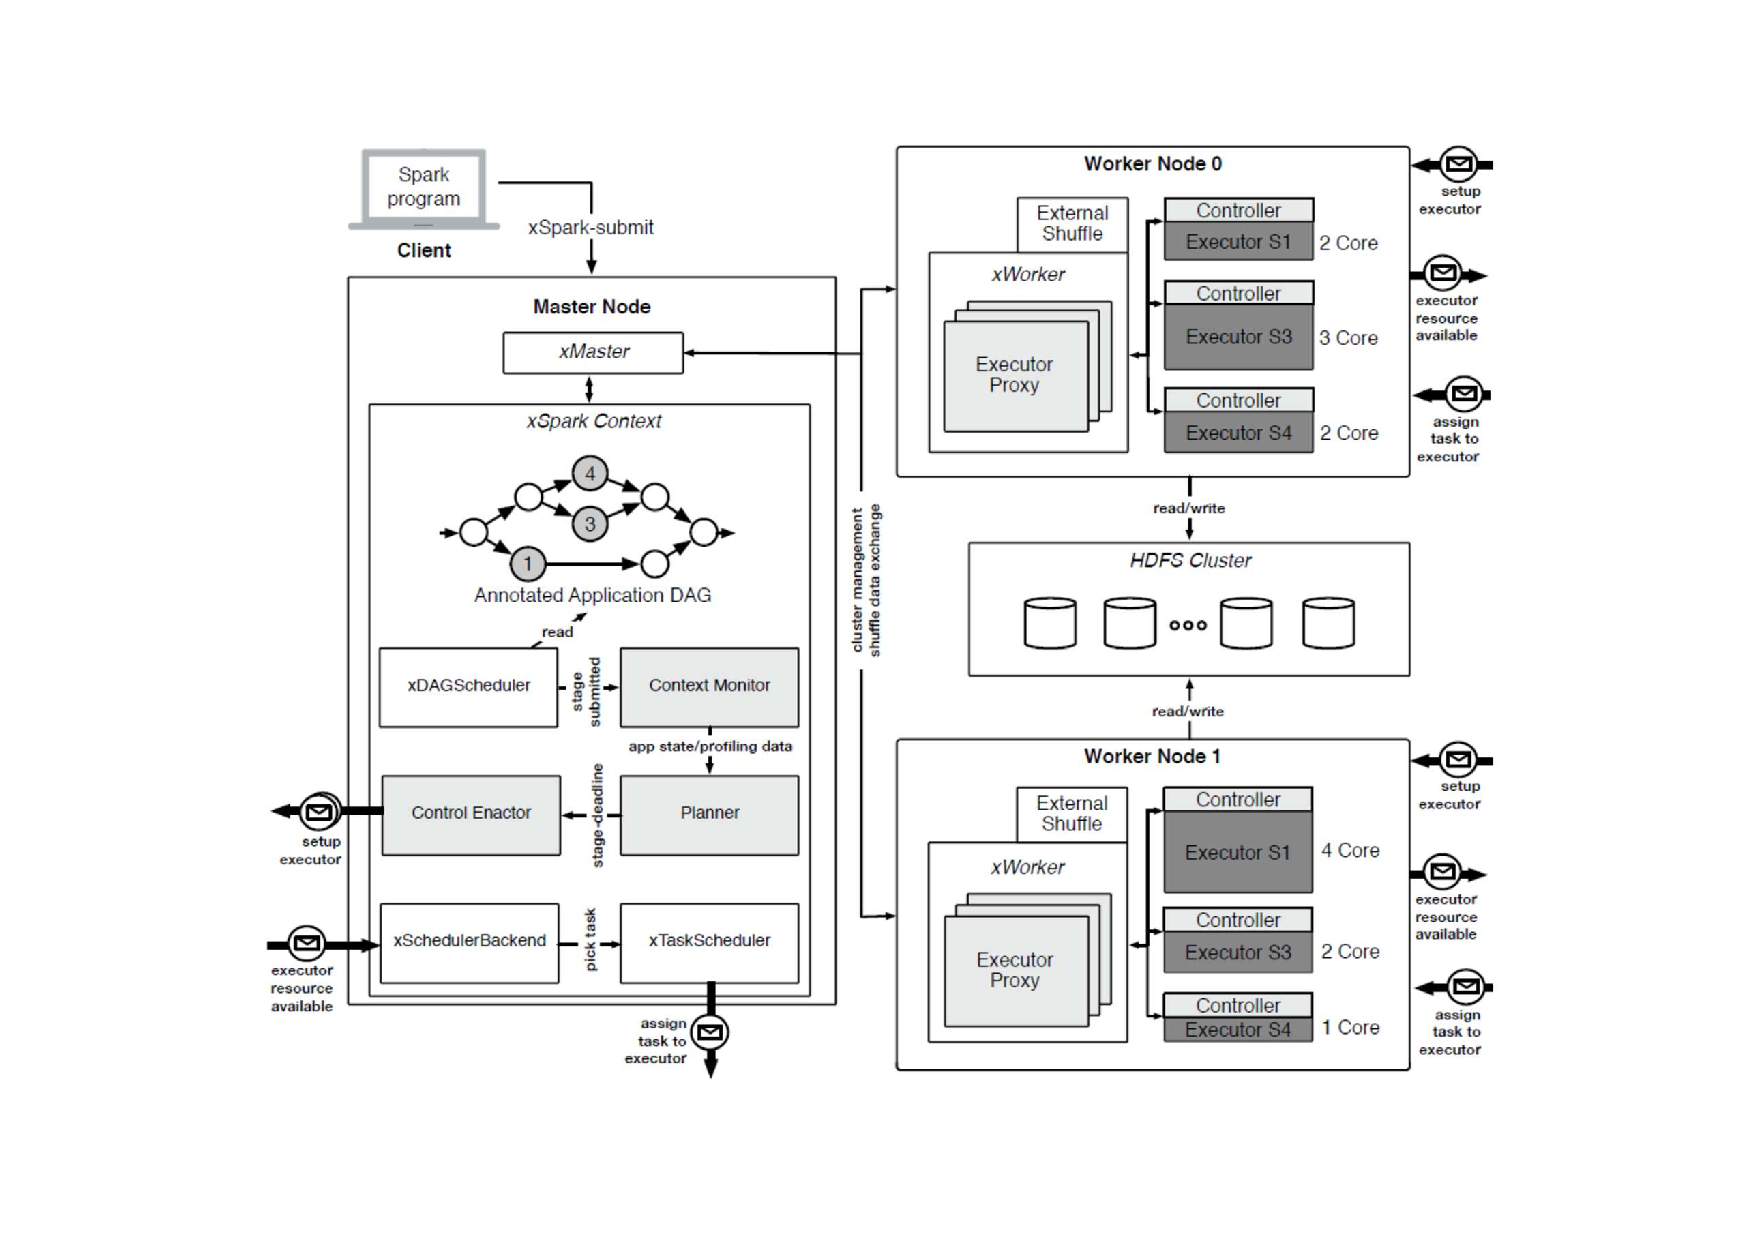
\includegraphics[width=\columnwidth]{Images/xspark_architecture.pdf}  
	\caption[Architecture of xSpark.]{Architecture of xSpark. New components are represented in light grey boxes, meanwhile those that start with an x are the modified ones. In dark grey are represented the containerized components (the executors).}
	\label{fig:xSparkArchitecture}
\end{figure}
\section{Architecture}\label{sec:architecture}

To achieve the objectives of xSpark, the architecture and processing model of Spark have been modified. In Figure 2.2 we can se how xSpark architecture differs from Spark. The principal architectural change introduced by xSpark is an increased focus on stages. Instead of considering entire applications, xSpark reasons on per-stage deadlines. 

xSpark instantiates an executor per stage per worker, instead of a single executor per worker for all the stages that will be executed. This way the resources that are allocated to a single executor only impact the performance of the stages that are associated with it, this leads to a fine grained control over the different stage, and thus on the entire application. When 
multiple stages are run in parallel, multiple executors can be running on the same worker node. When a stage is submitted for execution, one executor per worker is created and bound to that stage. This way computation and data are equally spread across the entire cluster.

Thanks to containers, xSpark can isolate the execution of the different executors that are running on the same worker node and achieve quick, fine-grained resource provisioning. On average, containers can be modified in less than one second, allowing a more precise way of
allocating cores.
Users submit applications and their deadlines to the master node using the submit command. This creates an \textit{xSparkContext} on the master node, containing a\textit{xMaster} object that is used to manage the cluster and that knows all the resources that are available on each worker
node. A \textit{xSparkContext} is composed by six components:
\begin{itemize}
	\item\textit{xDagScheduler} schedules the stages according to the application’s \plan. The submitted stage is enriched with the information obtained during the profiling phase
	\item\textit{ContextMonitor} monitors the progress of the application, taking into account stage scheduling and completion. It also stores information about the performance of the execution, that will be later used to calculate the deadlines and the resources needed by upcoming stages
	\item\textit{Planner} is heuristics based and is used to calculate the deadlines and resources associated with a stage
	\item\textit{ControlEnactor} determines when a stage is ready to be executed, meaning there are enough resources (cores) and sufficient executors become available. It also has the duty of initializing the different executors.
	\item\textit{xSchedulerBackend} controls the stage execution. In particular it launches new tasks by taking into account the resources availability and registers their completion
	\item\textit{xTaskScheduler} also controls stage execution, with the goal of allocating tasks to the available cores to optimize data locality. 
	In general, the closer a data partition required by a task is to the task’s executor, the better.
\end{itemize}

xSpark also modified the worker nodes. Each node contains a \textit{xWorker} that connects to a \textit{xMaster}, generates local controllers for the executors, and controls the evolution of its executor by dynamically scaling their resources. xWorker creates an \textit{Executor Proxy} for each of the executors that are running on its node. These proxies are placed between the executors and the \textit{xSchedulerBackend}, and are used to monitor the execution progress of the stage assigned to the executors. It is important to remember that each executor focuses on a single stage at a time. The heuristic calculates how many tasks must be executed by each of the executors of the same stage, the strategy is to have an equal number of tasks assigned to each of the executors. This way the deadline assigned to each of the executors coincides with the deadline of their stage. This allows the different executors of the same stage to
not be synchronized. Native Spark instead requires that executors with free resources spontaneously require new tasks to execute from the master node. 

Every xWorker uses an External Shuffle Service. Native Spark moves data across the cluster in different ways. If the data is stored on executor’s memory, then the executor itself manages the data exchange. If the data is stored on an external storage system (e.g., HDFS cluster),
they can be retrieved by using different communication protocols. If the data is stored in the internal storage of a worker node, then the data is managed by the External Shuffle Service. Notice that this is not the default, but xSpark adopts this technique to be able to assign
zero CPU cores to an executor, without loosing the ability to read data, since it is effectively not performed by the executor but by the external service.

\section{Heuristic}\label{sec:heuristic}
xSpark uses a heuristic to compute per-stage deadlines and to estimate how many cores must be allocated for a stage to successfully fulfill the deadline. In order to do this, at submission time the user is asked to specify three parameters: i) the application deadline, ii) the cluster size, and iii) the number of cores per worker node. Before executing the application, xSpark performs a feasibility check given the available resources.

When a stage is submitted for execution, its deadline is computed
\[deadline(sk) = \dfrac{\alpha\cdot ApplicationDeadline - SpentTime}{weight(sk)}\]
where $SpentTime$ is the time already spent for execution and $\alpha$ a
value between 0 and 1 that xSpark uses to be more conservative with
respect to the provided ApplicationDeadline. The weight is computed
\[\begin{cases}
w1(sk) = \#(RemainingStages + 1)\\
w2(sk) = \dfrac{{\Sigma}_{{a}_{i=k}}^{k+{w}_{1}}duration(s_i)}{duration(sk)}\\
weight(sk) = \beta\cdot w1(sk) + (1 - \beta) \cdot w2(sk)\\
\end{cases}\]
where w1 is the number of stages still to be scheduled (s included)
and w2 is the rate between the duration of s and the duration of the
remaining stages (s included).
xSpark then proceeds to estimate how many cores are needed to execute the stage:
\[estimatedCores(sk) = \lceil {\dfrac {inputRecords(sk)}{deadline(sk) \cdot nominalRate(sk)}}\rceil\]

where inputRecords is the number of records that will be processed by sk and nominalRate is the number of records processed by a single core per second in stage sk.

Since xSpark controls the resource allocation of a stage before and during the execution, the maximum amount of allocable cores needs to be greater than the estimated one, in order to be able to accelerate when progressing slower than expected 
\[maxAllocableCores(sk) = overscale \cdot estimatedCores(sk)\]
The final step is to determine the initial number of cores that should be assigned to the different executors, xSpark distributes the cores equally amongst the available workers by creating one executor per stage per worker. In this way, it is guaranteed that executor performances will be equal, and that xSpark can compute the same deadline for all the executors. The initial number of cores per executor is computed as
\[initCorePerExec(sk) = \lceil\dfrac {maxAllocableCores(sk)}{overscale \cdot cq \cdot numExecutors}\rceil\cdot cq\]
where $numExecutors$ is the number of executors and $cq$ is the $core\  quantum$, a constant that defines the quantization applied to resource
allocation, the smaller this value is, the more precise the allocation.

\section{Controller}\label{subsec:controller}
Each containerized executor has an associated local controller, whose goal is to fulfill the per-stage deadline taking into account external disturbances by dynamically allocating CPU cores. The controllers use control theory, with no heuristic involved.

The centralized control loop determines the desired stage duration, the maximum and the initial number of cores that should be assigned to the executors and the number of tasks that must be processed. Local controllers adjust the number of allocated cores, according to
the work that has already been accomplished.

Executors that are dedicated to different stages are implicitly independent, and thus their controllers are also independent. The executors that are running in parallel on the same stage must complete the same amount of work (number of tasks) in the same desired time.
This means that local controllers are independent and do not need to communicate among themselves. Moreover, the heuristic is relegated outside the local controller, so that it cannot compromise the controller’s stability.
\begin{figure}
	\centering
	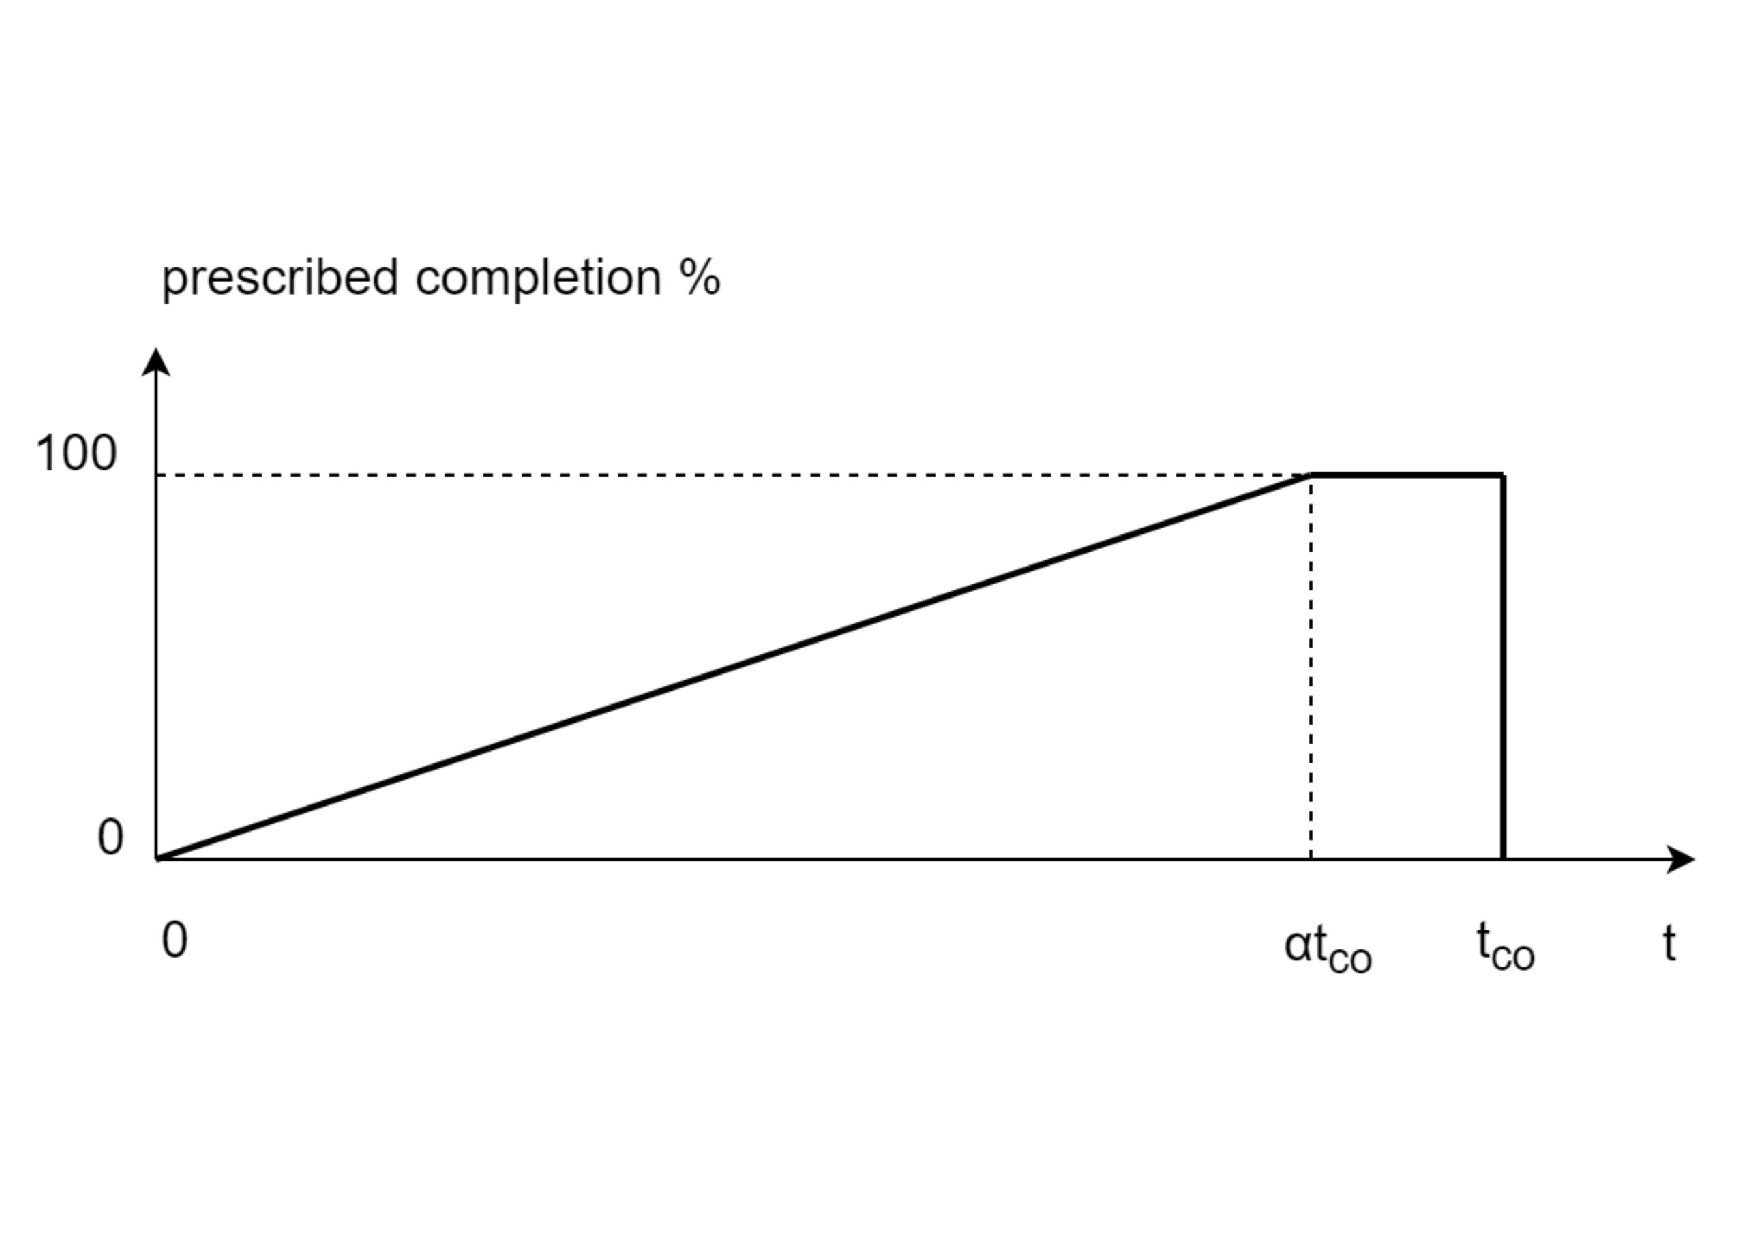
\includegraphics[width=\columnwidth]{Images/exec_controller_set_point.pdf}  
	\caption[Set point generation for an executor controller.]{Set point generation for an executor controller.}
	\label{fig:execControllerSetPoint}
\end{figure}
\begin{figure}
	\centering
	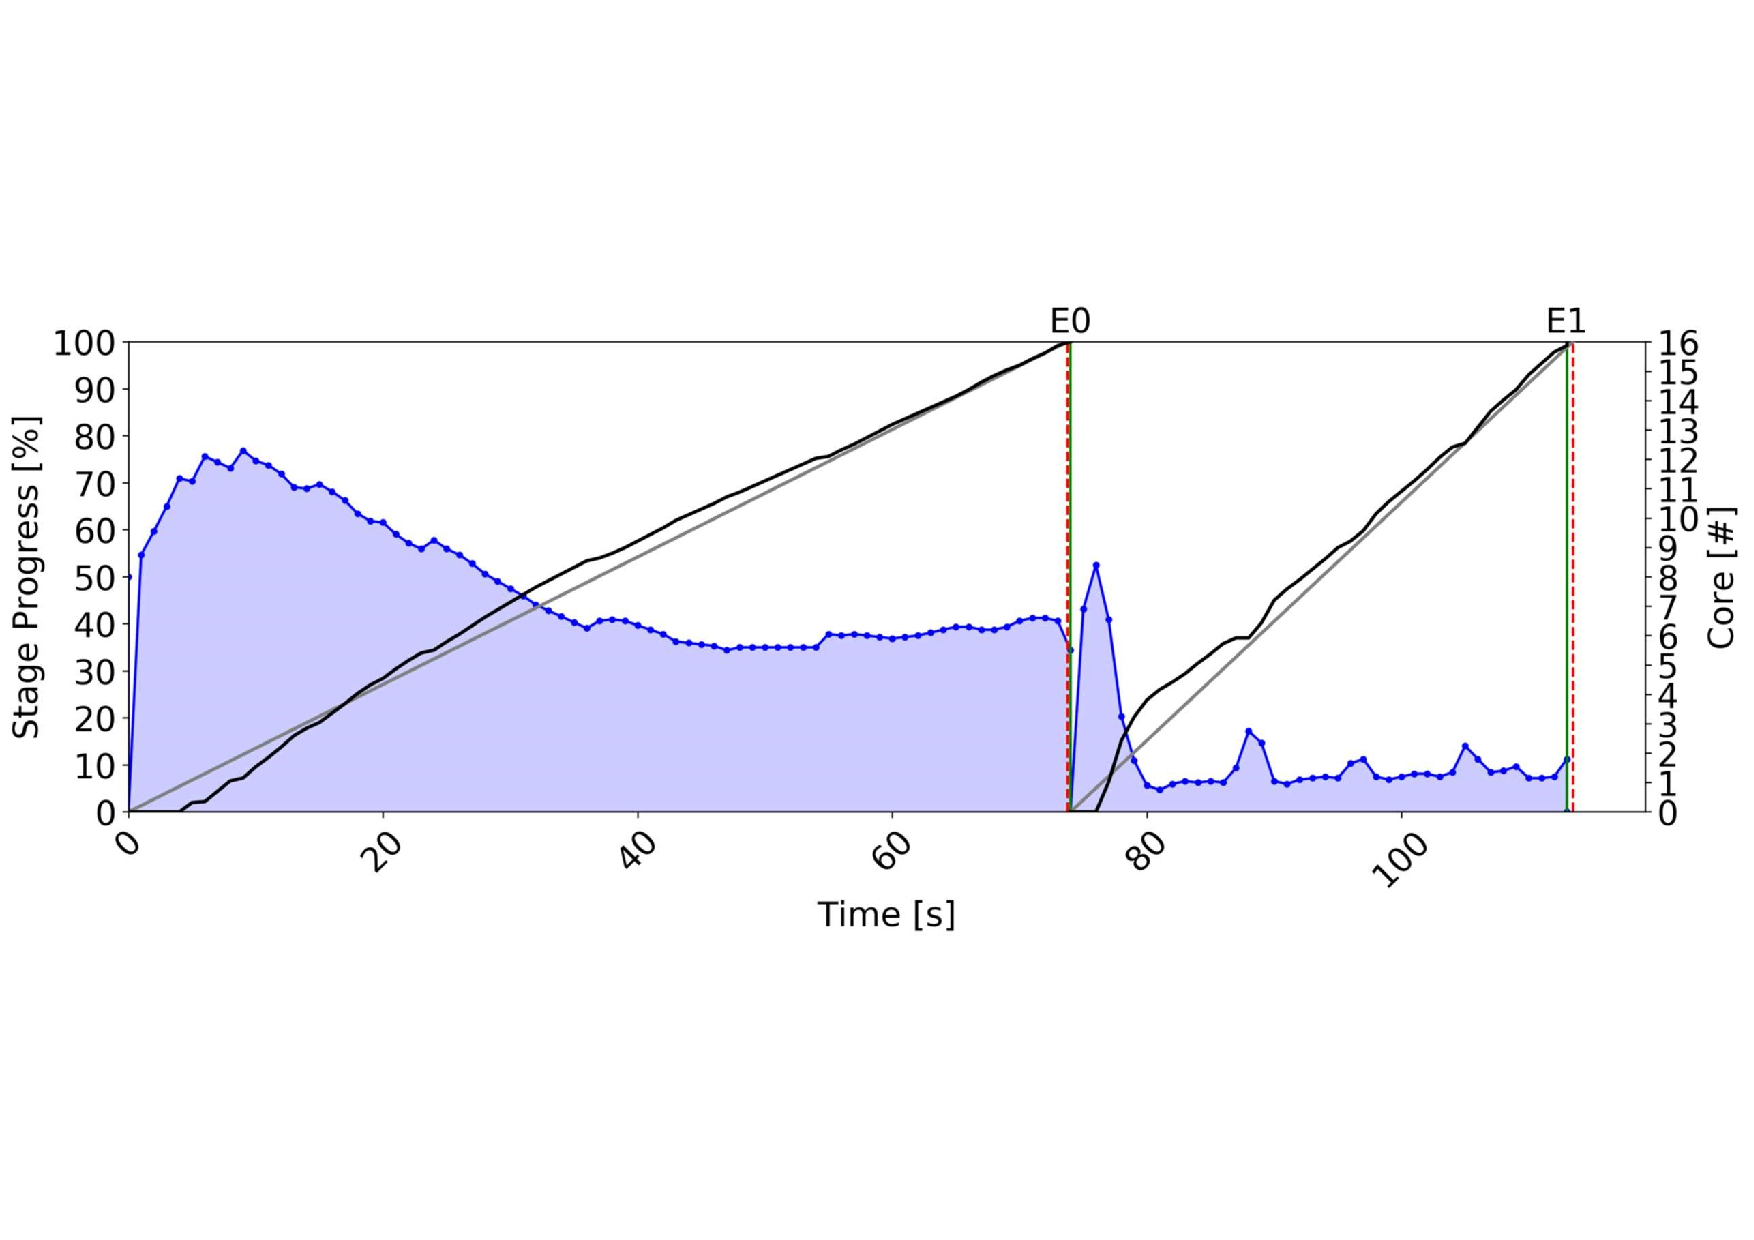
\includegraphics[width=\columnwidth]{Images/xspark_chart_agg_by_key.pdf}  
	\caption[xSpark chart aggrregate-by-key.]{CPU cores allocated to the application aggregate-by-key running on a xSpark worker node. The blue line represents the allocated cores over the time, gray and black line are desired and actual progress rate respectively. Green line represents the obtained stage ending, while dashed red line is the desired one.}
	\label{fig:xsparkChartAggByKey}
\end{figure}

In the controller, the progress set point is chosen based on the desired completion time. Its value is received from the centralized control loop. In \MyFig{fig:execControllerSetPoint} we see the prescribed completion percentage, in particular t\textsubscript{co} is the desired completion time and  $\alpha \in \left(0,1\right]$ is a configuration parameter used to determine how much earlier we are willing to complete the execution with respect to requested deadline,In order to track the set point ramp, we need to use a Proportional plus Integral (PI) controller.
As a result, the discrete-time controller in state space form reads:
\[\begin{cases}
x_{C}(k) = x_{C}(k - 1) + (1 - a)(a _{\%}^{o}(k - 1) - a _{\%}(k - 1))\\
c(k) = Kx_{C}(k) + K(a _{\%}^{o} - a _{\%}(k))\\
\end{cases}\]
where $(a _{\%}^{o}$ is the prescribed progress percentage at each $k$ control
step and a $_{\%}$ is the accomplished completion percent at each $k$ control
step. Notice that it is possible that the controller computes a negative value for $c(k)$, the CPU cores that need to be allocated. To fix this problem $c(k)$ must be clamped between a minimum $_{cmin}$ and a maximum $c_{max}$. To maintain consistency, we need to recompute the state $x_{C}(k)$ as 
\[x_{C}(k) = \dfrac{c(k)}{K} - a _{\%}^{o}(k) + a _{\%}(k)\] 

In \MyFig{fig:xsparkChartAggByKey} the cores allocated to an application executor running
on a worker node are shown. The running application is \textit{aggregateby-
key} and is composed by two stages. The black line represents the
progress of the stage, meanwhile the gray one is the desired progress
rate. The goal of the controller is to reduce the error, i.e., the distance
between the two lines. We want the black line to follow as much as
possible the gray line.
 
	%\chapter{Methodology} \label{chap:Methodology}
\begin{flushright}{\slshape    
   Science, my boy, is made up of mistakes, but they are mistakes
   which it is useful to make, because they lead little by little
   to the truth}. \\ \medskip --- \citeauthor{verne_journey:1957}
   \citetitle{verne_journey:1957} \citeyear{verne_journey:1957}
\end{flushright} 

\lettrine[lines=4]{\textcolor{purple}{B}}{ig} data applications are widely used in the industry and research fileds. Specialized   distributed frameworks are used to execute these applications on clusters of computers, very often made by cloud computing resources, like virtual machines and virtual storage. Apache Spark is probably the most popular big data processing framework. Spark organizes computations in directed acyclic graphs (DAG's) and its declarative API offers the capability to make transformations to datasets and return results to the client program, usually a standard Java, Python or Scala application. 

Spark starts executing a program by identifying jobs, delimited by the presence of actions in the code, and stages (within jobs), delimited by operations that require data to be shuffled (i.e., moved among executors), thus breaking locality. Indeed, Spark distinguishes
between narrow and wide transformations specifically for this purpose; the former do not shuffle data (e.g., map, filter, etc.), while the latter do (e.g., reduceByKey, etc.). Spark “identifies” all the operations that are to be executed, up to the first action, and
materializes them as a directed acyclic graph (DAG). The DAG is not the control-flow graph of the job’s code. It does not contain branches and loops since they were already resolved during the execution of the driver program. The DAG defines the execution order among stages, and defines the extent to which stages can be executed in parallel. For each job, Spark computes a DAG also called \textit{Parallel Execution Plan} (\plan) to maximize the parallelism while executing an application. In fact, a stage is, by definition, executed in parallel, and also different stages can be executed at the same time. For this reason, Spark materializes \plans as directed acyclic graphs of stages while the complete \model of an application is simply the sequence of the \plans of its jobs .A Spark application is usually composed by several jobs executed using a LIFO queue, therefore the \model of a Spark application is composed by the sequence of the \plans generated by the application jobs (an action corresponds to a job). In fact, Spark does not "compile" the code of the driver program to generate the application \model but it incrementally generates it as soon as an action is reached.

\section{Problem Statement}\label{sec:problem_statement}
Our goal is to support efficient execution of deadline-based QoS constrained multi-{\model} Spark applications, i.e. applications whose execution flow cannot be represented with a single \plan, and whose actual execution flow is only known at application execution runtime. In addition, the execution time is constrained by a user-defined deadline, that is the expected duration of the application.

The literature contains several works exploring adaptation capabilities, formal guarantees or response time estimation for Spark applications based on their \plan-based structure~\cite{dSpark, xsparkreport, Quattrocchi2018}, assuming that the \plan of the application does not change with respect to different data input or parameters. However, the \plan uniqueness assumption does not hold if conditional branches or loops are present in the control flow of the client program.

This is particularly relevant in Spark because of the possibility of evaluating
partial results through actions. In fact, these values can be used in the code as part of conditional expressions that can create branches in the control flow graph. In this cases the conditional branches govern the final structure of the \plan and also the operations that form a stage while loops influence the number of repetition of either transformations, stages or actions. 

Our solution is based on xSpark, a modified version of Apache Spark, developed at Politecnico di Milano~\cite{xsparkreport, Quattrocchi2018}, that has demonstrated the capability to execute deadline-constrained single-\plan applications by using resources more efficiently than  Spark would do in running the same applications. xSpark is able to use less resources than native Spark and can complete executions with less than 1\% error in terms of set deadlines.

Given all the above stated, in order to reach our objective of efficiently running deadline-based QoS constrained multi-\plan Spark applications, we need to positively answer to the following Research Questions:
\begin{enumerate}[\boldmath$RQ_1 $] 
	\item - [Effectiveness]:  Does our solution effectively control the execution of the Spark applications?
	\item - [Efficiency]:  To what extent can our solution improve the resource allocation capabilities of \cSpark, given it used a single, constant \plan?
\end{enumerate}
Most of the approaches in the literature (e.g., \cite{gibilisco2016stage,Sidhanta2016, dSpark, nfm}) use the execution graph to reason on the work to do, the degree of parallelism, the duration of tasks, and other application-specific characteristics. They also assume that the graph does not change since many of the conditional  branches and loops are hidden in the code (e.g., filter, map). As said, this is wrong when the code contains explicit loop and conditional statements.

For example, one can think of a simple two-job application. The first job retrieves some records from a data source (e.g., a file) and filters them according to a given criterion; the second job sorts them and returns the first $x$ records. To avoid problems, one may constrain the execution of the second job to the fact that the cardinality $c$ of filtered records, that is, the result produced by the first job, is greater than zero. The execution graph would then comprise two jobs $if c \geq 0$; it would only comprise the first job otherwise. This simple example shows how Spark can return partial results ($c$) through actions to the driver program and use these results to evaluate conditional (loop) expressions, and thus produce different execution graphs.

To overcome this problem, \cSpark and many solutions~\cite{Sidhanta2016, dSpark} exploit an initial profiling phase to retrieve the execution graph and collect some performance metrics. Back to the simple example sketched above, the initial profiling would simply return the execution graph implied by the data used to run the application. This single choice impacts the quality of obtained results and there is currently no means to adjust the graph with respect to the different data.
Even if one adopts a conservative approach and retrieves the execution graph that corresponds to the worst case (i.e., two jobs in the previous example), this would result in over-allocating resources and/or over-estimating execution times. If one adopted the best case (one job), too few resources and too short execution time would be foreseen.

\begin{figure}[htbp]
	\begin{small}
		\begin{verbatim}
		1  from pyspark import SparkContext
		2  def run(numIterations, threshold):
		3    sc = SparkContext('local','example')
		4  	 x = sc.textFile(...).map(...).groupBy(...)
		5     .map(...).aggregate(...)
		6    y = sc.textFile(...).map(...).groupBy(...)
		7     .map(...).aggregate(...)
		8    if x > threshold and y > threshold:
		9      for i in range(numIterations):
		10       z = sc.parallelize(...).map(...).sort(...).take(10)
		11   if x > y:
		12       w = sc.parallelize(...).map(...).filter(...).count()
		\end{verbatim}
	\end{small}
	\caption{Example Spark application with conditional branches and loops.}
	\label{fig:xdag2-code}
\end{figure}


The execution graph can also depend on user parameters or local variables and they must be considered in a sound analysis. For example, Figure~\ref{fig:xdag2-code} shows the code of an example application that takes two input parameters \textit{numIterations} and \textit{threshold}; its execution graph depends on both user parameters and input dataset. The first two \textit{aggregate} jobs\footnote{In Spark \textit{aggregateByKey} is a transformation while \textit{aggregate} is an action.} are always executed (line $4$ and $6$) and the results are assigned to variables $x$ and $y$, respectively. Line $8$ checks if both variables are greater than \textit{threshold}. If it is the case, a \textit{take} job (line $10$) is repeated \textit{numIterations} times (\verb#for# loop). Finally, if $x > y$ (line $11$) \textit{count} (line $12$) is executed. 

This simple code corresponds to four possible execution graphs (Figure~\ref{fig:xdag2}): i) the sequence of the two \textit{aggregate}s  (if the two conditional statements are both false) ii) the sequence of the two \textit{aggregate}s and \textit{take} repeated \textit{numIterations} times (if the first conditional statement is true and the second is not) iii) the sequence of the two \textit{aggregate}s and \textit{count} (if the second conditional statement is true but not the first), and iv) the concatenation of the two \textit{aggregate}s, \textit{take} repeated \textit{numIterations} times, and \textit{count} (if both conditional statements are true).

\begin{figure}[t]
	\centering
	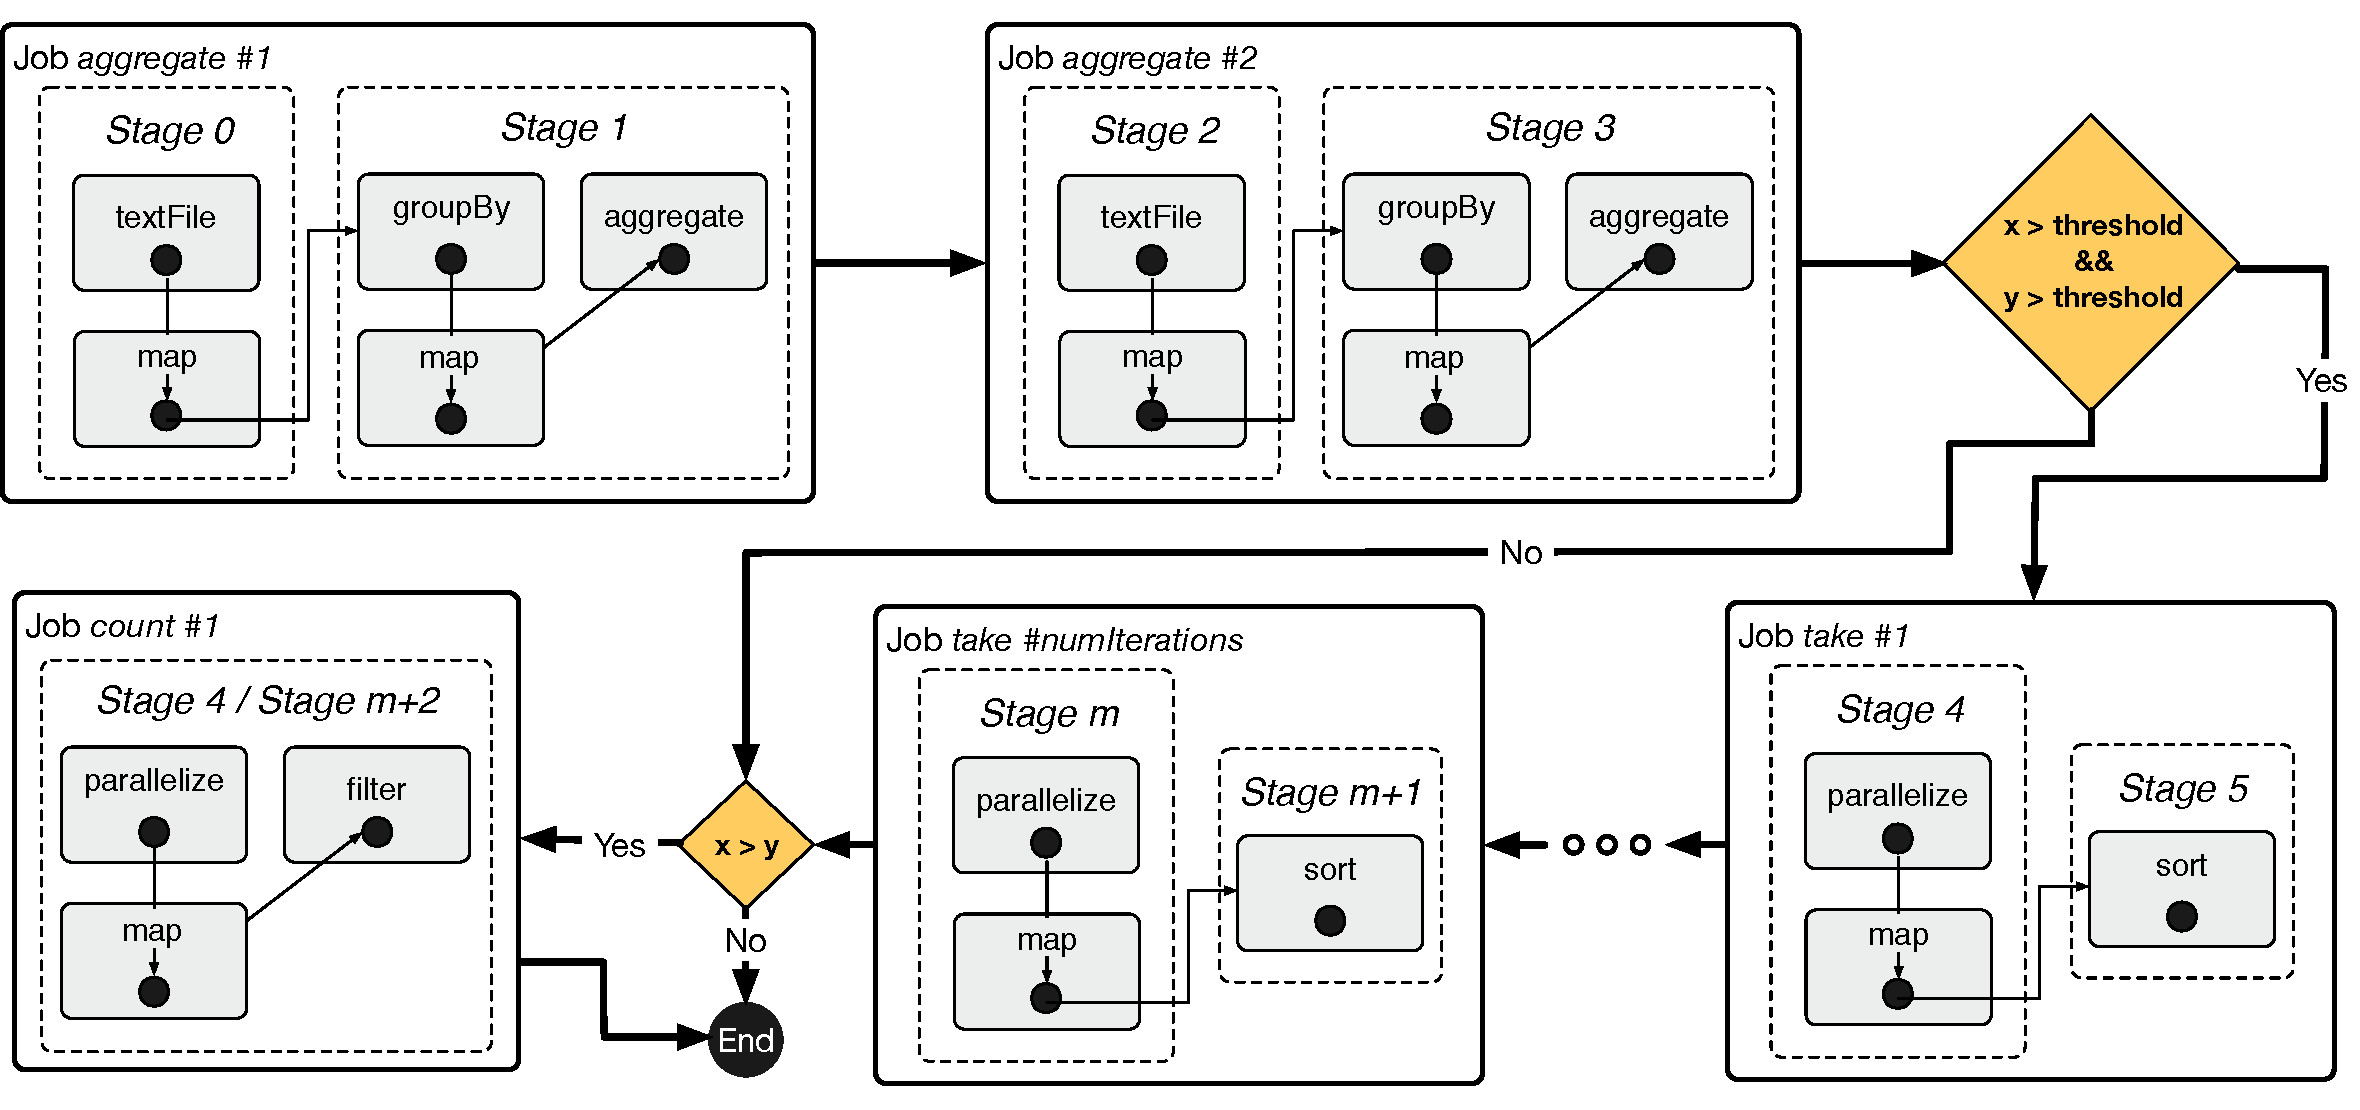
\includegraphics[width=1\columnwidth]{images/xdag2.pdf}
	\caption{The four  \plans of the application of Figure~\ref{fig:xdag2-code}.}
	\label{fig:xdag2}
\end{figure}

\section{Solution Overview}\label{sec:solution_overview}
This section contains a functional level description of the proposed solution, of its components and their interactions to make the solution work.

This thesis work presents \tool, a toolchain providing the capability to manage the efficient execution of deadline-based QoS constrained multi-\plan Spark applications. 

\tool is the result of the integration of \dSymb, a tool exploiting symbolic execution techniques to generate the path condition associated to each possible {\plan}s produced by different inputs and parameters, with (a modified version of) xSpark.
 Moreover, \tool generates a launcher with a synthesized dataset for each \plan and an artifact to retrieve the feasible {\plan}s given a set of symbolic variables  resolved to a value. Finally, we integrated this approach with xSpark, an extension of Spark that can control the duration of Spark applications according to specified deadlines through dynamic resource allocation. 
 
The evaluation shows that \approach is able to effectively extract all the DAGs generated by Spark applications and that xSpark reduces the number of deadline violation thanks to the presented integration.
In the remainder of this section we will go through a more detailed explanation of the solution's components and how they cooperate to provide the final result.

\subsection{\approach}\label{sec:symb}

In this section we describe \approach, \emph{Symbolic Execution-driven Extraction of Parallel Execution Plans}, an original combination of lightweight symbolic execution and search-based test generation that allows us to extract the \model of Spark applications. A \model  associates each control-flow path of the target application with the \plan generated by its execution, the relative profiling data, and the path condition that activates the path. 

\approach consists of four main phases: i) it relies on a lightweight symbolic execution of the driver program of the Spark application to derive a representative set of execution conditions of the control-flow paths in the program; ii) it exploits those execution conditions with a search-based test generation algorithm, to compute sample input datasets that make each path execute; iii) it executes the target application with those datasets as input, to profile the \plan generated by each path, and synthesize the \model accordingly; iv) it generates an artifact called \textit{GuardEvaluator} that returns the feasible \plans given a partial set of concrete values of the symbolic variables.
%In particular, for each  control-flow path analyzed during symbolic execution, the \model stores the execution conditions of the path, the Spark-DAGs of the jobs that Spark executes throughout the path, and the relevant execution-time data profiled during the execution. 
We exploit the information in the \model computed with \approach to extend \cSpark (see Section~\ref{sec:control}) with the ability of tuning its adaptation strategy according to the worst-case behaviour of the application. At runtime, our extended version of \cSpark exploits the \textit{GuardEvaluator} to refine the control policy by recomputing the worst-case estimation every time the current worst-case refers to a program path for which the execution condition stored in the \model becomes unsatisfiable.
%
Below, we describe each phase of \approach in detail.

\subsection{Lightweight Symbolic Execution}
\approach relies on a lightweight symbolic execution of the driver program of the Spark application to identify the execution conditions of the feasible program paths of the driver program. To this end, \approach
models with unconstrained symbolic values the results of the parallel computation jobs issued in the driver program, 
% that correspond to the jobs defined in the driver program, 
thus abstracting from the details of those computations, and symbolically  analyzes the dependencies of the program paths on these symbolically modeled results.
%This simplifies the symbolic execution  working under the very conservative (though possibly imprecise) assumption that every distributed computation launched during the execution of the driver program may yield any possible result.  
\approach leaves for the subsequent test generation phase the burden of identifying concrete input datasets that make the parallel computation jobs encompassed in the driver program yield results that satisfy the path constraints identified during symbolic execution.

This section formalizes the lightweight symbolic execution algorithm of \approach for a simple imperative programming language in which all operations are either assignments of program variables or assume operations. The assignments are in the form \texttt{x := e}, where \texttt{x} is a program variable and \texttt{e} is an expression of values of program variables. The assume operations are in the form \texttt{assume(c)}, where \texttt{c} is a condition on the values of program variables, with the semantics that the program continues to execute only if the condition \texttt{c} evaluates to \emph{true}. 
A program in this language defines a transition system with a finite set of program locations $L \triangleq \{\ell_1, \ell_2, \dots, \ell_n\}$, a specified initial location $\ell_{init} \in L$, and a transition relation $T \triangleq \{t  \equiv \langle\ell, op \rightarrow \ell'\rangle\}$ that states the semantics of the program that can move from $\ell\in L$ to $\ell'\in L$ by executing a valid assignment or assume  operation $op$.

Two special classes of assignments, that is, assignments of the form \texttt{x := parallel\_op($\dots$)} and \texttt{x~:= aggregation\_op($\dots$)}, respectively, define parallel computations. 
The assignments \texttt{x := parallel\_op($\dots$)} assign the variable \texttt{x}
of the special type \emph{Dataset} to the result of the
expression \texttt{parallel\_op($\dots$)}, which in our context can refer to evaluating any of the parallel computation operations allowed in Spark (e.g., \texttt{map}, \texttt{filter}, \texttt{reduceByKey}).
The assignments \texttt{x~:= aggregation\_op($\dots$)} assign the variable \texttt{x}
to the result of a data aggregation operation, e.g., \texttt{count}, \texttt{collect}, etc, evaluated against a dataset computed in parallel fashion. 
%Our symbolic execution algorithm does not interpret the possible input parameters of these operations, such as for example the parameters in the the expression \texttt{data.map($\lambda$)} that receives and input dataset \texttt{data} and a function \code{$\lambda$} to execute in parallel fashion. 

Figure~\ref{fig:symbex} defines the symbolic execution algorithm of \approach. We denote the symbolic states computed during the analysis with $s \equiv \langle \ell, vv, pc\rangle$, being $\ell$ the program location to which this symbolic state refers, $vv$ the set of program variables assigned so far, and $pc$ (the path condition) the path constraint due to the assume operations traversed so far. The algorithm starts from the initial state $s\_{init} \equiv \langle \ell_{init}, \emptyset, true\rangle$ (no variable assigned, unconstrained path), and unfolds the transitions of each program path by recursively executing the atomic step $s'\gets SE(s, t)$ of Figure~\ref{fig:symbex}, where $s'$ is the state reached from $s$ when executing the transition $t$. 


\begin{figure*}
	\newcommand{\code}[1]{ \text{\texttt{#1}}}
	\tiny
	\[SE(s\equiv\langle \ell, vv, pc\rangle, t\equiv\langle \ell, op \rightarrow \ell'\rangle) \triangleq 
	\begin{cases}
	
	\langle \ell', vv[\code{x} \gets \llbracket \code{e}\rrbracket_{vv})], pc\rangle
	& \text{ if } 
	op \equiv \code{x := e}\\
	
	\langle \ell', vv, pc \wedge \llbracket \code{c}\rrbracket_{vv}\rangle
	& \text{ if } 
	op \equiv \code{assume(c)}\\
	
	\langle \ell', vv[x \gets \delta], pc\rangle
	& \text{ if } 
	op \equiv \code{x := \textit{parallel\_op}($\dots$)} \text{ e.g. }
	\begin{cases}
	\code{sparkCtx.textFile($\dots$)}\\ % \code{sparkCtx.parallelize($\dots$)}\\
	\code{data.map($\lambda$)}\\ \code{data.filter(\textit{$\lambda$}))}\\ \code{data.reduceByKey(\textit{$\lambda$})}\\ \code{data.groupBy($\lambda$)}\\ \code{data.flatMap($\lambda$)}\\ \code{data.aggregateByKey($\lambda$)}\\ \code{data.cartesian($\lambda$)}\\ 
	\dots
	\end{cases}\\
	
	
	\langle \ell', vv[x \gets \alpha_\ell], pc\rangle
	& \text{ if } 
	op \equiv \code{x := \textit{aggregate\_op}($\dots$)}  \text{ e.g. }
	\begin{cases}
	\code{data.count()}\\ \code{data.collect()}\\ \code{data.take(n)}\\ \dots
	\end{cases}\\
	
	\end{cases}
	\]
	
	\caption{Symbolic execution algorithm of \approach.}
	\label{fig:symbex}
	\normalsize
\end{figure*}

Figure~\ref{fig:symbex} specifies the algorithm as a list of four cases. The first two cases describe the classic symbolic execution algorithm that handles 
\begin{inparaenum}[(i)]
	\item the assignment operations  \texttt{x := e} by setting the variable \texttt{x} to the value of expression \texttt{e} in the current state %($x \gets \llbracket e\rrbracket_{vv}$), and 
	\item the assume operations \texttt{assume(c)} by conjoining the current path condition with the value of condition \texttt{c} in the current state ($pc \wedge \llbracket \texttt{c}\rrbracket_{vv}$). 
	%
	The last two cases in Figure~\ref{fig:symbex} define the abstract modeling of the assignments that involve parallel operations:  
	\item the assignments \texttt{x~:= parallel\_op($\dots$)} result in setting the variable \texttt{x} to the unique symbolic value $\delta$, which we use to symbolically model every dataset accessed and computed in the program; \item the assignments \texttt{x := aggregation\_op($\dots$)} result in setting the variable \texttt{x} to a new unconstrained symbolic value $\alpha_\ell$ that model the result of the aggregation operator called at the program location $\ell$.  (For simplicity the figure omits the further incremental index that we use to symbolically model the results of subsequent assignments at a location that is traversed multiple times in the same program path.)
\end{inparaenum}

The right part of Figure~\ref{fig:symbex} exemplifies a set of both \texttt{parallel\_op} and \texttt{aggregation\_op} operations. These examples include Spark operations that appear in any listing in this paper. Beyond these examples, with reference to the RDD Programming Guide~\cite{RDDGuide:online:2019}, the  \texttt{parallel\_op} operations of Figure~\ref{fig:symbex} encompass the complete list of \emph{transformation} and \emph{shuffle} operations, while the  \texttt{aggregation\_op} operations encompass all \emph{action} operations. 

An important remark about the algorithm is that the conditions of the assume operations defined in the driver program cannot explicitly predicate on the internal state of variables of type \emph{Dataset}. In fact, although the variables of type \emph{Dataset} undergo parallel computations, the data produced with these computations may propagate in the driver program only indirectly, as the result of invoking some \texttt{x := aggregation\_op(...)} operation. Thus, the assume operations in the driver program may predicate only on variables assigned as \texttt{x := e} and \texttt{x := aggregation\_op(...)}. 
This guarantees that the symbolic value $\delta$ that models the assignments \texttt{x~:= parallel\_op(...)} never appears in a path condition, which is the reason why we can embrace the simplification of using this single symbolic value to abstractly model all the datasets that the target driver program may manipulate. 

\approach uses the algorithm Figure~\ref{fig:symbex} to symbolically analyze the paths of the target driver program, and returns the path condition computed for each path. As usual in symbolic execution, we use a constraint solver to check if any path condition formula becomes unsatisfiable at some point of the analysis, and dismiss the analysis of the program paths with unsatisfiable path conditions.  Our current \approach prototype implements the algorithm described in this section on top of the symbolic executor JBSE~\cite{braione:jbse:fse:2016} that relies on the constraint solver Z3~\cite{demoura:z3:tacas:2008}.

For example, for the Spark application in Figure~\ref{fig:xdag2-code}, when analyzing the paths of the driver program that do not enter the loop at line~9, 
\ (let $\alpha_5$ and $\alpha_7$ be the symbols that represent the results of the \texttt{aggregate} actions at line~5 and line~7, respectively, and $thresh$ and $iters$ the symbols that represent the input values of parameters \texttt{threshold} and \texttt{numIterations}, respectively) \approach computes the path conditions:
\begin{itemize} 
	\item \(\alpha_5 \le thresh \wedge \alpha_5 > \alpha_7\);
	\item \(\alpha_5 \le thresh \wedge \alpha_5 \le \alpha_7\);
	\item \(\alpha_5 > thresh \wedge \alpha_7 \le thresh \wedge \alpha_5 > \alpha_7\);
	\item \(\alpha_5 > thresh \wedge \alpha_7 > thresh \wedge iters \le 0 \wedge  \alpha_5 > \alpha_7\);
	\item \(\alpha_5 > thresh \wedge \alpha_7 > thresh \wedge iters \le 0 \wedge  \alpha_5 \le \alpha_7\);
	
\end{itemize}
%
while it identifies the unsatisfiable path condition \(\alpha_5 > thresh \wedge \alpha_7 \le thresh \wedge \alpha_5 \le \alpha_7\).

For programs with loops, like the one in the figure, \approach bounds the iterations of the loops to an user-defined maximum value, thus guaranteeing to have to symbolically analyze a finite amount of paths. 

\subsection{Search-Based Test Generation}
\approach exploits the path conditions identified with symbolic execution as above, to generate test cases (a test case for each path condition) comprised of input values and input datasets that make the target Spark application concretely execute  the  paths of the driver program that correspond to the path conditions. The goal is to use these test cases in the next phase of \approach,  to profile the behavior of the \plan generated by the execution each path of the driver program.

To generate a test case for a given path condition,  \approach incrementally explores the space of the possible test cases in search-based fashion, steering the search with a fitness function that quantifies the extent to which each incrementally considered test case is close to (or far from) satisfying the path condition at hand. Below, we first describe the \approach search algorithm in detail, and then explain the 
test execution sandbox that the algorithm uses to speed up the execution of the test cases. 

\subsubsection{Search Algorithm}
The \approach search algorithm generates test cases that call the target application with 
the inputs (both the input parameters and the input datasets) assigned to concrete values (both concrete values of the parameters and and concrete datasets). 
The algorithm samples the possible values of the inputs in the style of \emph{genetic algorithms}. It starts with generating a \emph{population} of test cases comprised of randomly picked inputs, and then \emph{evolves} from the initial population, by incrementally generating a series of next-generation populations, each obtained 
by manipulating the test cases in the previous-generation population with \emph{mutation} and \emph{crossover} operators. 
Mutation operators generate new test cases by randomly modifying some inputs of a test case of the previous-generation population. The crossover operators generate new test cases as the children of some pair of test cases of the previous-generation population, by conjoining inputs taken from either test case of the pair. 

The \approach fitness function quantifies the goodness of each generated test case with respect to the goal of satisfying a path condition, one of those identified in the previous phase, yielding a value that we interpret as the distance of the current test case from a satisfying test case: If the fitness function yields a distance of 0, the current test case is indeed a satisfying test case, and the search algorithm returns it as result; Otherwise, the fitness function yields a value greater than zero that the search algorithm exploits to comparatively order the test cases of the current population.  The search algorithm proceeds with probabilistically favouring the application of mutation and crossover operators to 
test cases with lower distance from the goal, thus increasing the chances to eventually converge to a satisfying test case. 

In detail, \approach computes the fitness of a test case with respect to a path condition as follows. First, it executes the test case, and collects the results of the Spark aggregation actions that the driver program executes thereby. Next, it evaluates the path condition for the valuation of the symbolic values induced by the execution of the test case, that is, by assigning the symbolic values that model input parameters to the concrete values set in the test case, and the symbolic values that model results of aggregation actions (the $\alpha_\ell$ symbols of Figure~\ref{fig:symbex}) to the corresponding results collected while executing the test case. If the test case does not execute an aggregation action referred in the path condition, we assign the corresponding symbol to the special value $Undef$. Then, if there are no $Undef$ symbols, and if the path condition evaluates to $true$ for the concrete assignment induced by the test case, then the fitness is zero: indeed the test case satisfies the path condition. Otherwise, the fitness is the positive value yielded by the following formula (let $t$ be the test case, and $pc$ be the path condition):
%
\[fitness(t, pc\equiv c_1\wedge c_2\wedge\dots\wedge c_n) = \sum_{i=1}^{n} distance(t, c_i)\]

\noindent where $c_i$ are the atomic conditionals in the path condition $pc$, and the function $distance$ that appears in the summation recursively computes the distance of each atomic conditional from being satisfied. In turn, the function $distance$ is defined as follows (let $c \equiv o_1 \bowtie o_2$ be a conditional, where $\bowtie$ is a comparison operator and $o_1$, $o_2$ are operands, either literals or symbolic expressions): 

\[distance(t, c) \triangleq 
\begin{cases}
0, \text{~~~~if } t(o_1) \bowtie t(o_2)= true\\
1, \text{~~~~if } t(o_1)= \text{Undef } \vee t(o_2)= \text{Undef}\\
1-\dfrac{1}{1 + |t(o_1)-t(o_2)| + \epsilon},  \text{~~~~otherwise}
\end{cases}\]

\noindent where $t(o_1)$ and $t(o_2)$ are the values of the operands $o_1$ and $o_2$, respectively, for the concrete assignments set in the test case $t$,  $t(o_1)$ and $t(o_2)$ are set to $Undef$ if they depend on any symbol assigned to $Undef$ after executing the test case, and $\epsilon$ is an arbitrary small number.

We make the following remarks about the \approach fitness function. Function $distance$ yields always a value in the interval [0, 1], and thus the overall $fitness$ ranges in the interval [0, n] for a path condition with $n$ atomic conditionals. Function $distance$ yields zero (first case in the formula) for satisfied conditionals, and thus the overall $fitness$ is zero only for a test case that satisfies all conjuncts, that is, a satisfying test case, as expected.  Function $distance$ yields the maximum value 1 (second case in the formula) for conjuncts that refer to any symbol assigned to $Undef$, and thus the overall $fitness$ is never zero if it depends on any symbol assigned to $Undef$, as expected. Function $distance$ yields values increasingly closer to zero (third case in the formula) if the operands of the referred conditional evaluate to increasingly mutually-closer values, meaning that the corresponding test cases are missing the satisfaction of the conditional for increasingly smaller amounts. Thus, the overall $fitness$ is  increasingly closer to zero, the higher the number of satisfied or close-to-be-satisfied conditionals, as expected.

%Come funzione di fitness usiamo la path condititon di ogni path, e quindi la soluzione ottima e' un insieme di dataset popolati con dati che, quando eseguiti dal driver program, portano ad eseguire il path identificato dalla path condition. 


\subsubsection{Test Execution Sandbox}
Each fitness evaluation issued in the above search algorithm requires, at least in principle,  the execution of the parallel application under test, which can quickly become computationally infeasible in consideration of the many test cases that the algorithm generates during the search. To address this issue, the \approach search algorithm executes the test cases in a test execution sandbox that specializes the RDD-typed datasets of the target Spark application as a custom type of datasets that we call \emph{sparse diversity data (\sparsedata) datasets}. 

A \sparsedata dataset  synthetically represents a RDD object with many data points that hold the same value. In \sparsedata format, a dataset is modelled as a list of data blocks, each with two attributes, namely, \texttt{size} and \texttt{value}: A data block with \texttt{size} equal to $s$ and \texttt{value} equal to $v$ 
stands for a set of $s$ data points, all with the same value $v$.  \approach uses the \sparsedata format to model datasets in which the amount of distinct values is significantly much smaller than the overall amount of values in the dataset. For example, a dataset with $20^9$ data points in which half of the data points have value 100 and the other half -100 can be very concisely represented with a \sparsedata dataset with two data blocks, both with \texttt{size} equal to $10^9$, and \texttt{value} equal to 100 and -100, respectively. 

The test execution sandbox recasts the computation of the parallel operations allowed for the RDD objects (e.g., operations like \texttt{map}, \texttt{filter}, \texttt{reduceByKey}, etc.) to sequencial operations executed against the data blocks in the \sparsedata objects. For example, a  \texttt{map($\lambda$)} transformation executed on a \sparsedata dataset $D$ with data blocks $[b_1, b_2, ..., b_n]$ yields a new \sparsedata dataset $D'$ with data blocks $[b'_1, b'_2, ..., b'_n]$  such that, for all $i=1..n$,  $b'_i.size := b_i.size$ and $b'_i.value := \lambda(b_i.value)$.
Similarly, a  \texttt{filter($\lambda$)} transformation on $D$ 
yields $D''$ with the subset of data blocks of $D$ that satisfy the condition $\lambda(b_i)$. Yet, a \texttt{count()} action on $D$ yields the value $\sum^i b_i.size$ as result. Our \sparsedata objects handle all transformations and actions defined in the RDD Programming Guide~\cite{RDDGuide:online:2019}. 


The crossover and mutation operators of the \approach search algorithm manipulate the input \sparsedata datasets of the target application by modifying, adding and removing data blocks (mutation operators) or combining the data blocks from the \sparsedata datasets in the parent test cases (crossover operator). 
Our current \approach prototype implements the search algorithm described in this section based on the SUSHI test generation framework~\cite{braione:combining:issta:2017, braione:sushi:icse:2018}. SUSHI converts the path conditions generated with JBSE in fitness functions as the ones described in this section, and adapts the test genetic search procedure of the tool EvoSuite~\cite{fraser:evosuite:tse:2013} to use these fitness functions. 

For example, with reference to a path condition computed for the Spark application in Figure~\ref{fig:xdag2-code}, e.g., one of those reported in the previous section, \approach may compute a test case resembling like the following one
\begin{verbatim}
Test:
1  threshold = 152;
2  numIterations = 0;
3  D1 = new SDD(size = 1000000, value = 721);
4  D2 = new SDD(size = 3000000, value = 814);
5  setInputTextFile(..., D1);
6  setInputTextFile(..., D2);
7  run(numIterations, threshold);
\end{verbatim}
that sets the input parameters \texttt{threshold}  and \texttt{numIterations} to concrete values (lines~1--2), builds two SDD datasets, both with a single data block (lines~3--4), sets these datasets as the input files that the application will read as input (lines~5--6), and executes the application with these inputs. 

\[a = \lceil b + c\rceil\]

\subsection{Synthesis of the \model}

\approach uses the test cases generated with the search algorithm, to execute the target Spark application, and profile the \plan generated by the execution of each path of the driver program. In this phase, \approach replaces the \sparsedata datasets that appear in the test cases yielded by the search algorithm with proper RDD datasets comprised of the same amount of data. It executes the test cases against the target application in fully parallel fashion. While executing each test case, \approach stores the \plan that the Spark engine produces before starting each parallel execution job, and monitors the parallel execution of the jobs to collects the timing data that are relevant for  the control policy. 

\approach builds the \model model as a set of triples \[\langle pc \rightarrow \plans, times\rangle\] where each triple represents the sequence of \plans  and the timing data --- $times$ --- associated with the execution of the test case that corresponds to the path condition $pc$. 

Together with the \model, \approach produces an an artifact that we call \textit{GuardEvaluator} that takes as input partial set of concrete values of the symbolic variables, evaluates the path conditions of  triples in the \model against these values, identifies which path conditions evaluate to $false$ for these values, and  
returns as output the subset of the \model with only the triples with non-falsified path conditions. In the control policy that we define in the next section, we invoke the guard evaluator at runtime, feeding it with the concrete values of the input parameters and incrementally with the concrete values of the executed actions, to stay tuned on the program paths that are possibly reachable at every intermediate execution state. 


\approach addresses the possible incompleteness of either its symbolic execution and search phase as follows. As we already commented above, in the symbolic execution phase, \approach analyzes the loops in the program up to a finite (user-configured) amount of iterations, and the analysis may thus produce incomplete results if it indeed happens to dismiss some program path (if any) that iterates any loop more than that amount. In this case, \approach tracks the path conditions $\hat{pc}$ that correspond to the interrupted prefix of the non-analyzed paths, and stores these path conditions in the \model as special triples with missing data \(\langle \hat{pc} \rightarrow \emptyset, -\rangle\).  Similarly, if the search algorithm fails to converge to the optimal solution for some path condition $\tilde{pc}$, \approach stores corresponding triples with missing data \(\langle \tilde{pc} \rightarrow \emptyset, -\rangle\). These special triples in the \model allow the control policy described in the next section to anticipate when an un-profiled path is going to be executed at runtime, and take decisions to mitigate the impact of these unforeseen situations. 


\subsection{xSpark$_{\text{\textit{\textbf{SEEPEP}}}}$}
This section describes how \dSymb integrates within \cSpark: the resulting tool-chain is called \tool. \dSymb produces the 
path conditions associated with the different \plans of the application, a set of test cases for each \plan for profiling, and a \textit{GuardEvaluator} to allow \cSpark to select the most appropriate \plan at runtime. At each execution step, \textit{GuardEvaluator} always returns the \plans whose associated path conditions still hold true. 


\begin{figure}[tbhp]
	\centering
	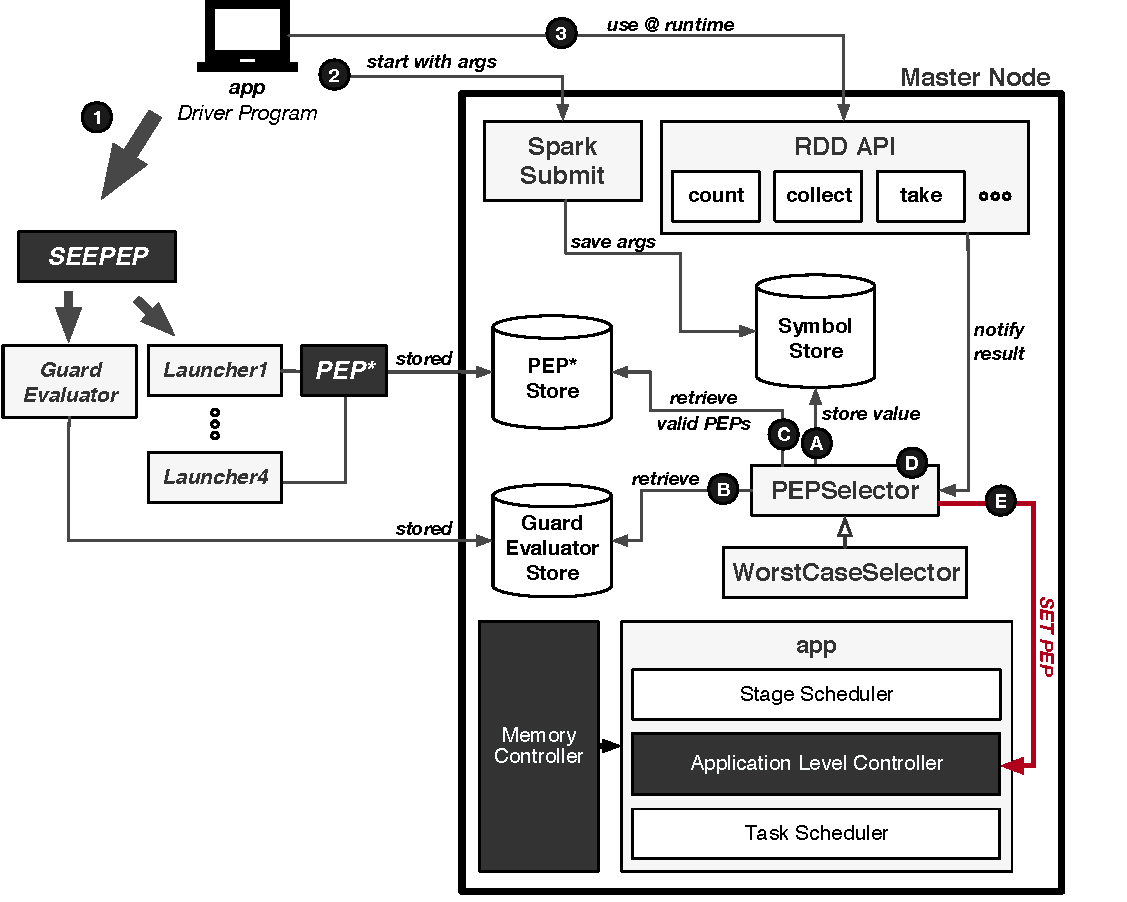
\includegraphics[width=\columnwidth]{images/xsparksymb}
	\caption{\tool}
	\label{fig:xsparkdagsymb}
\end{figure}

Figure~\ref{fig:xsparkdagsymb} shows the main elements of the tool-chain and exemplifies it on profiling and controlling the example application of Figure~\ref{fig:xdag2} ---\textit{app}, hereafter. As first step, \dSymb generates the $4$ ($n$, in general) launchers, which activate the four ($n$) \plans of the program, and an application specific \textit{GuardEvaluator}. 

The new toolchain associates each \plan to its path condition, it uses the generated launchers to obtain the profiling data of each \plan and synthesize the \model for the application that is then stored in the master node in component \textit{PEP* Store}. Finally the generated \textit{GuardEvaluator}, which implements a common interface to be dynamically instantiated and used without a static import in the source code of \cSpark, is also stored in the master node (component \textit{GuardEvaluator Store}).

After this phase, $app$ can be executed and controlled by \cSpark. 
Since the application parameters can be part of a path condition as symbols, we modified component \textit{SparkSubmit} to store their values. A symbol is identified by application name, action name, code line in the driver program, and a counter to take multiple executions into account  (i.e., loops or recursive functions). 

At runtime, everytime an action is executed, that is, a result is computed and returned to the driver program, our modified version of the  \textit{RDD API} notifies component \textit{PEPSelector} that a new result is available. This component is in charge of selecting the \plan and its profiling data then used by \textit{Application Level Controller} to compute the local deadlines for the next stages and thus to provision resources. \textit{PEPSelector} saves computed results into component \textit{Symbol Store}, retrieves an instance of the dedicated \textit{GuardEvaluator}, and feeds it with all the symbols resolved 
by the aforementioned results. \textit{GuardEvaluator} returns the list of \plan whose path conditions still hold.

This means, for example, that at the beginning of the execution of function \textit{run} of $app$, four \plans are valid since neither $x$ nor $y$ have been resolved to a value. The job at line $4$ produces the value of $x$ and if the value is less than or equal to $threshold$,  the if statement of line $8$ is not evaluated. Therefore, even if the value of $y$ is still unknown, \textit{GuardEvaluator} only returns two \plans, that is, the only two \plans whose path conditions still hold: it excludes all the path conditions that depends on the expression $x > threshold$). This way, since the \plan is updated constantly, \cSpark becomes aware of what has been actually done, and can use this information to refine resource provisioning.  

Note that \textit{PEPSelector} receives all the valid \plans and computes the next \plan to use. This selection can be customized by the user. Currently, we always select the worst-case \plan, that is, the \plan with the greatest number of remaining stages to be conservative and minimize deadline violations. If one wanted to optimize different performance indicators (e.g., deadlines are not strict and used resources must be minimized), the selection could privilege a \plan that corresponds to an average case instead of the worst one. 
	\chapter{Problem Statement and Solution Overview} \label{chap:ProblemAndSolution}
\begin{flushright}{\slshape    
   Science, my boy, is made up of mistakes, but they are mistakes
   which it is useful to make, because they lead little by little
   to the truth}. \\ \medskip --- \citeauthor{verne_journey:1957}
   \citetitle{verne_journey:1957} \citeyear{verne_journey:1957}
\end{flushright} 

\lettrine[lines=4]{\textcolor{purple}{B}}{ig} data applications are widely used in the industry and research fileds. Specialized   distributed frameworks are used to execute these applications on clusters of computers, very often made by cloud computing resources, like virtual machines and virtual storage. Apache Spark is probably the most popular big data processing framework. Spark organizes computations in directed acyclic graphs (DAG's) and its declarative API offers the capability to make transformations to datasets and return results to the client program, usually a standard Java, Python or Scala application. 

Spark starts executing a program by identifying jobs, delimited by the presence of actions in the code, and stages (within jobs), delimited by operations that require data to be shuffled (i.e., moved among executors), thus breaking locality. Indeed, Spark distinguishes
between narrow and wide transformations specifically for this purpose; the former do not shuffle data (e.g., map, filter, etc.), while the latter do (e.g., reduceByKey, etc.). Spark “identifies” all the operations that are to be executed, up to the first action, and
materializes them as a directed acyclic graph (DAG). The DAG is not the control-flow graph of the job’s code. It does not contain branches and loops since they were already resolved during the execution of the driver program. The DAG defines the execution order among stages, and defines the extent to which stages can be executed in parallel. For each job, Spark computes a DAG also called \textit{Parallel Execution Plan} (\plan) to maximize the parallelism while executing an application. In fact, a stage is, by definition, executed in parallel, and also different stages can be executed at the same time. For this reason, Spark materializes \plans as directed acyclic graphs of stages while the complete \model of an application is simply the sequence of the \plans of its jobs .A Spark application is usually composed by several jobs executed using a LIFO queue, therefore the \model of a Spark application is composed by the sequence of the \plans generated by the application jobs (an action corresponds to a job). In fact, Spark does not "compile" the code of the driver program to generate the application \model but it incrementally generates it as soon as an action is reached.

\section{Problem Statement}\label{sec:problem_statement}
Our goal is to support efficient execution of deadline-based QoS constrained multi-{\model} Spark applications, i.e. applications whose execution flow cannot be represented with a single \plan, and whose actual execution flow is only known at application execution runtime. In addition, the execution time is constrained by a user-defined deadline, that is the expected duration of the application.

The literature contains several works exploring adaptation capabilities, formal guarantees or response time estimation for Spark applications based on their \plan-based structure~\cite{dSpark, xsparkreport, Quattrocchi2018}, assuming that the \plan of the application does not change with respect to different data input or parameters. However, the \plan uniqueness assumption does not hold if conditional branches or loops are present in the control flow of the client program.

This is particularly relevant in Spark because of the possibility of evaluating
partial results through actions. In fact, these values can be used in the code as part of conditional expressions that can create branches in the control flow graph. In this cases the conditional branches govern the final structure of the \plan and also the operations that form a stage while loops influence the number of repetition of either transformations, stages or actions. 

Our solution is based on xSpark, a modified version of Apache Spark, developed at Politecnico di Milano~\cite{xsparkreport, Quattrocchi2018}, that has demonstrated the capability to execute deadline-constrained single-\plan applications by using resources more efficiently than  Spark would do in running the same applications. xSpark is able to use less resources than native Spark and can complete executions with less than 1\% error in terms of set deadlines.

Given all the above stated, in order to reach our objective of efficiently running deadline-based QoS constrained multi-\plan Spark applications, we need to positively answer to the following Research Questions:
\begin{enumerate}[\boldmath$RQ_1 $] 
	\item - [Effectiveness]:  Does our solution effectively control the execution of the Spark applications?
	\item - [Efficiency]:  To what extent can our solution improve the resource allocation capabilities of \cSpark, given it used a single, constant \plan?
\end{enumerate}
Most of the approaches in the literature (e.g., \cite{gibilisco2016stage,Sidhanta2016, dSpark, nfm}) use the execution graph to reason on the work to do, the degree of parallelism, the duration of tasks, and other application-specific characteristics. They also assume that the graph does not change since many of the conditional  branches and loops are hidden in the code (e.g., filter, map). As said, this is wrong when the code contains explicit loop and conditional statements.

For example, one can think of a simple two-job application. The first job retrieves some records from a data source (e.g., a file) and filters them according to a given criterion; the second job sorts them and returns the first $x$ records. To avoid problems, one may constrain the execution of the second job to the fact that the cardinality $c$ of filtered records, that is, the result produced by the first job, is greater than zero. The execution graph would then comprise two jobs $if c \geq 0$; it would only comprise the first job otherwise. This simple example shows how Spark can return partial results ($c$) through actions to the driver program and use these results to evaluate conditional (loop) expressions, and thus produce different execution graphs.

To overcome this problem, \cSpark and many solutions~\cite{Sidhanta2016, dSpark} exploit an initial profiling phase to retrieve the execution graph and collect some performance metrics. Back to the simple example sketched above, the initial profiling would simply return the execution graph implied by the data used to run the application. This single choice impacts the quality of obtained results and there is currently no means to adjust the graph with respect to the different data.
Even if one adopts a conservative approach and retrieves the execution graph that corresponds to the worst case (i.e., two jobs in the previous example), this would result in over-allocating resources and/or over-estimating execution times. If one adopted the best case (one job), too few resources and too short execution time would be foreseen.

\begin{figure}[htbp]
	\begin{small}
		\begin{verbatim}
		1  from pyspark import SparkContext
		2  def run(numIterations, threshold):
		3    sc = SparkContext('local','example')
		4  	 x = sc.textFile(...).map(...).groupBy(...)
		5     .map(...).aggregate(...)
		6    y = sc.textFile(...).map(...).groupBy(...)
		7     .map(...).aggregate(...)
		8    if x > threshold and y > threshold:
		9      for i in range(numIterations):
		10       z = sc.parallelize(...).map(...).sort(...).take(10)
		11   if x > y:
		12       w = sc.parallelize(...).map(...).filter(...).count()
		\end{verbatim}
	\end{small}
	\caption{Example Spark application with conditional branches and loops.}
	\label{fig:xdag2-code}
\end{figure}


The execution graph can also depend on user parameters or local variables and they must be considered in a sound analysis. For example, Figure~\ref{fig:xdag2-code} shows the code of an example application that takes two input parameters \textit{numIterations} and \textit{threshold}; its execution graph depends on both user parameters and input dataset. The first two \textit{aggregate} jobs\footnote{In Spark \textit{aggregateByKey} is a transformation while \textit{aggregate} is an action.} are always executed (line $4$ and $6$) and the results are assigned to variables $x$ and $y$, respectively. Line $8$ checks if both variables are greater than \textit{threshold}. If it is the case, a \textit{take} job (line $10$) is repeated \textit{numIterations} times (\verb#for# loop). Finally, if $x > y$ (line $11$) \textit{count} (line $12$) is executed. 

This simple code corresponds to four possible execution graphs (Figure~\ref{fig:xdag2}): i) the sequence of the two \textit{aggregate}s  (if the two conditional statements are both false) ii) the sequence of the two \textit{aggregate}s and \textit{take} repeated \textit{numIterations} times (if the first conditional statement is true and the second is not) iii) the sequence of the two \textit{aggregate}s and \textit{count} (if the second conditional statement is true but not the first), and iv) the concatenation of the two \textit{aggregate}s, \textit{take} repeated \textit{numIterations} times, and \textit{count} (if both conditional statements are true).

\begin{figure}[t]
	\centering
	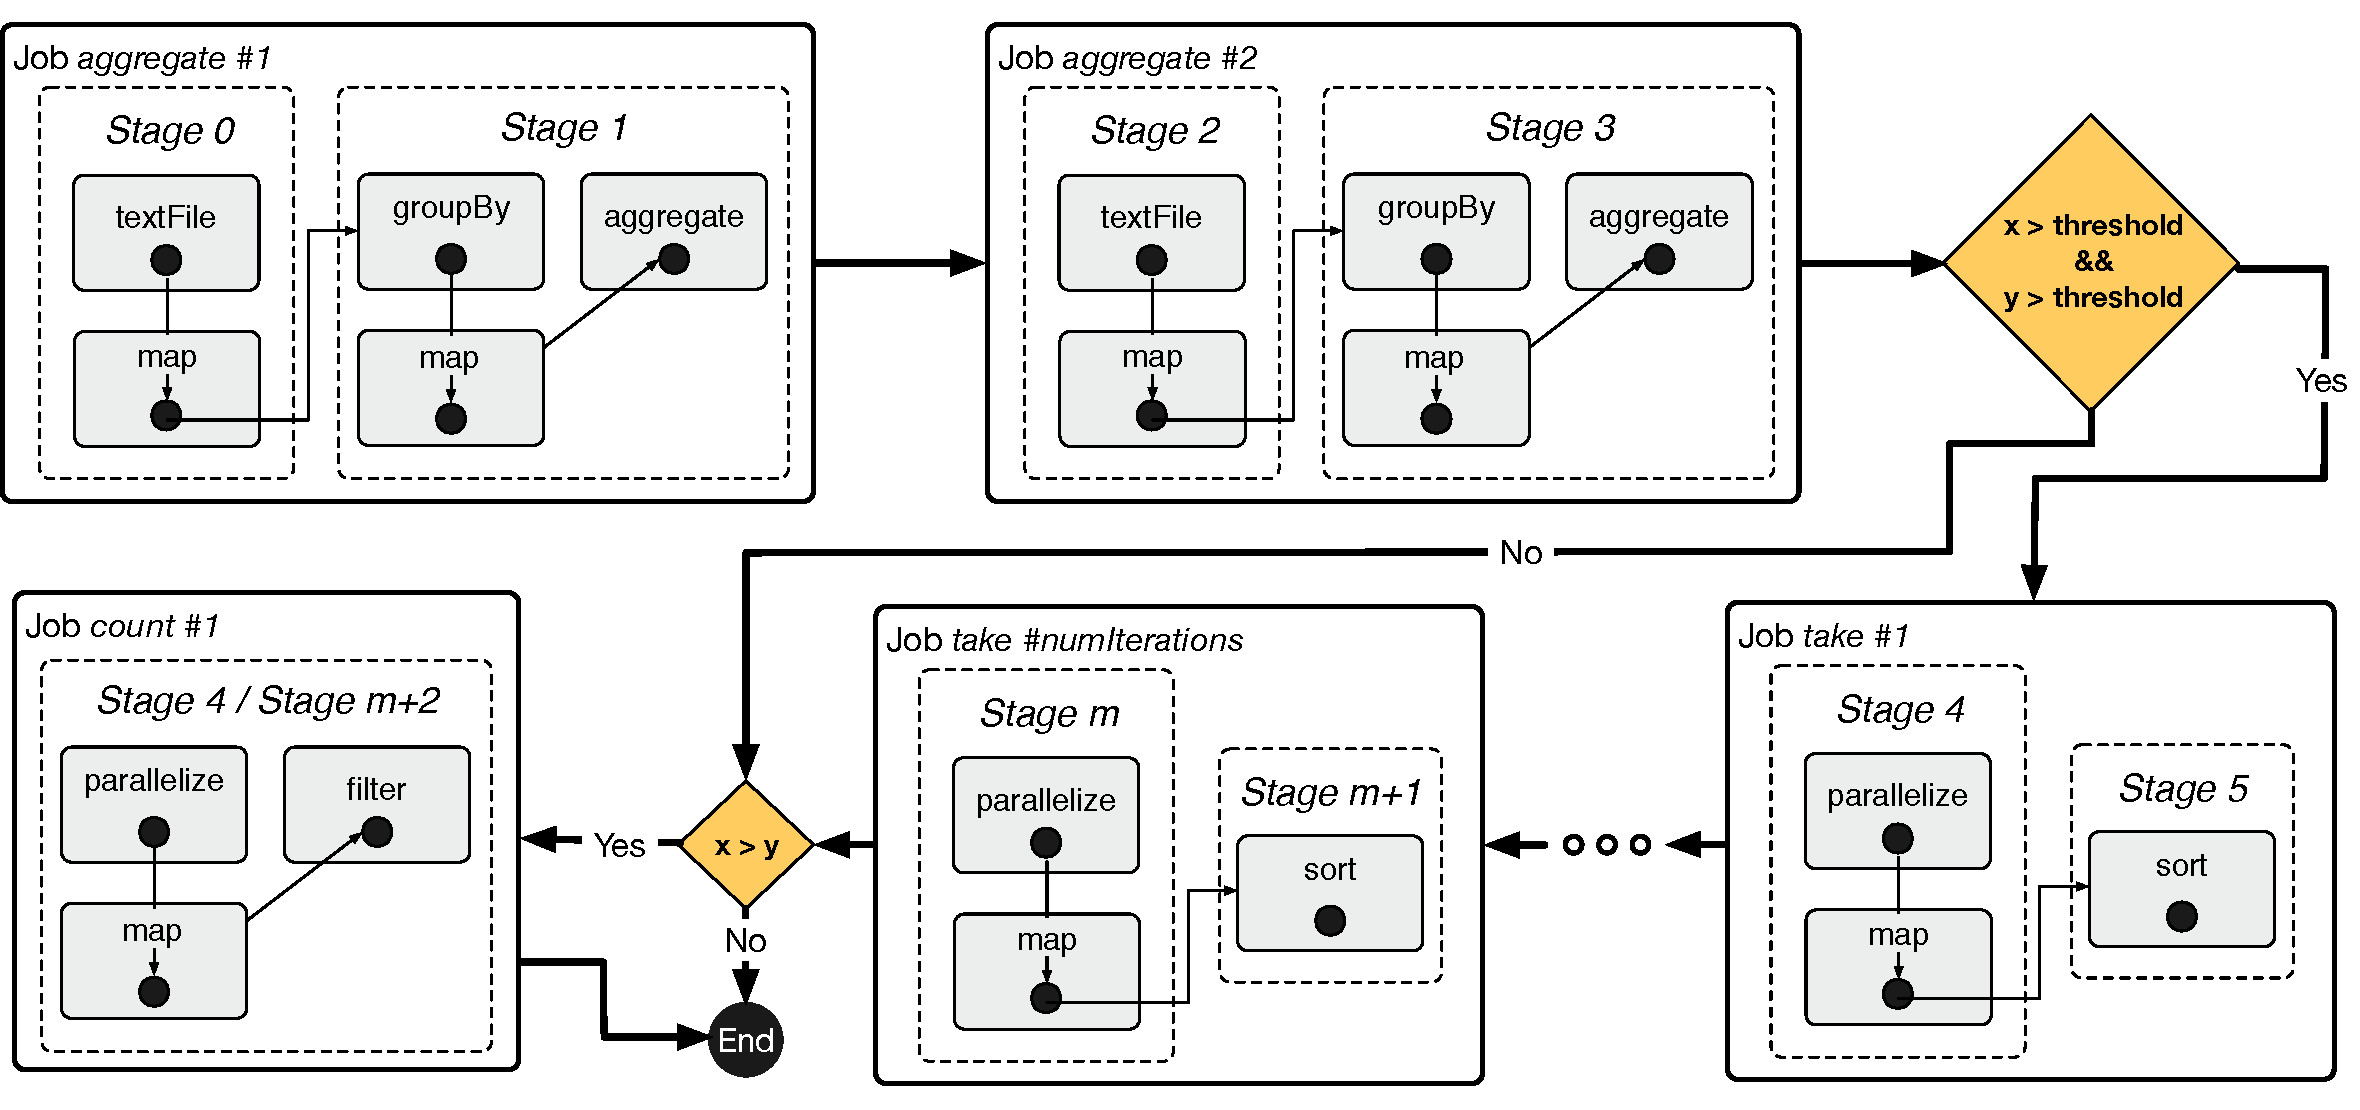
\includegraphics[width=1\columnwidth]{images/xdag2.pdf}
	\caption{The four  \plans of the application of Figure~\ref{fig:xdag2-code}.}
	\label{fig:xdag2}
\end{figure}

\section{Solution Overview}\label{sec:solution_overview}
This section contains a functional level description of the proposed solution, of its components and their interactions to make the solution work.

This thesis work presents \tool, a toolchain providing the capability to manage the efficient execution of deadline-based QoS constrained multi-\plan Spark applications. 

\tool is the result of the integration of \dSymb, a tool exploiting symbolic execution techniques to generate the path condition associated to each possible {\plan}s produced by different inputs and parameters, with (a modified version of) xSpark.
 Moreover, \tool generates a launcher with a synthesized dataset for each \plan and an artifact to retrieve the feasible {\plan}s given a set of symbolic variables  resolved to a value. Finally, we integrated this approach with xSpark, an extension of Spark that can control the duration of Spark applications according to specified deadlines through dynamic resource allocation. 
 
The evaluation shows that \approach is able to effectively extract all the DAGs generated by Spark applications and that xSpark reduces the number of deadline violation thanks to the presented integration.
In the remainder of this section we will go through a more detailed explanation of the solution's components and how they cooperate to provide the final result.

\subsection{\approach}\label{sec:symb}

In this section we describe \approach, \emph{Symbolic Execution-driven Extraction of Parallel Execution Plans}, an original combination of lightweight symbolic execution and search-based test generation that allows us to extract the \model of Spark applications. A \model  associates each control-flow path of the target application with the \plan generated by its execution, the relative profiling data, and the path condition that activates the path. 

\approach consists of four main phases: i) it relies on a lightweight symbolic execution of the driver program of the Spark application to derive a representative set of execution conditions of the control-flow paths in the program; ii) it exploits those execution conditions with a search-based test generation algorithm, to compute sample input datasets that make each path execute; iii) it executes the target application with those datasets as input, to profile the \plan generated by each path, and synthesize the \model accordingly; iv) it generates an artifact called \textit{GuardEvaluator} that returns the feasible \plans given a partial set of concrete values of the symbolic variables.
%In particular, for each  control-flow path analyzed during symbolic execution, the \model stores the execution conditions of the path, the Spark-DAGs of the jobs that Spark executes throughout the path, and the relevant execution-time data profiled during the execution. 
We exploit the information in the \model computed with \approach to extend \cSpark (see Section~\ref{sec:control}) with the ability of tuning its adaptation strategy according to the worst-case behaviour of the application. At runtime, our extended version of \cSpark exploits the \textit{GuardEvaluator} to refine the control policy by recomputing the worst-case estimation every time the current worst-case refers to a program path for which the execution condition stored in the \model becomes unsatisfiable.
%
Below, we describe each phase of \approach in detail.

\subsection{Lightweight Symbolic Execution}\label{sec:lightweight_symbolic_execution}
\approach relies on a lightweight symbolic execution of the driver program of the Spark application to identify the execution conditions of the feasible program paths of the driver program. To this end, \approach
models with unconstrained symbolic values the results of the parallel computation jobs issued in the driver program, 
% that correspond to the jobs defined in the driver program, 
thus abstracting from the details of those computations, and symbolically  analyzes the dependencies of the program paths on these symbolically modeled results.
%This simplifies the symbolic execution  working under the very conservative (though possibly imprecise) assumption that every distributed computation launched during the execution of the driver program may yield any possible result.  
\approach leaves for the subsequent test generation phase the burden of identifying concrete input datasets that make the parallel computation jobs encompassed in the driver program yield results that satisfy the path constraints identified during symbolic execution.

This section formalizes the lightweight symbolic execution algorithm of \approach for a simple imperative programming language in which all operations are either assignments of program variables or assume operations. The assignments are in the form \texttt{x := e}, where \texttt{x} is a program variable and \texttt{e} is an expression of values of program variables. The assume operations are in the form \texttt{assume(c)}, where \texttt{c} is a condition on the values of program variables, with the semantics that the program continues to execute only if the condition \texttt{c} evaluates to \emph{true}. 
A program in this language defines a transition system with a finite set of program locations $L \triangleq \{\ell_1, \ell_2, \dots, \ell_n\}$, a specified initial location $\ell_{init} \in L$, and a transition relation $T \triangleq \{t  \equiv \langle\ell, op \rightarrow \ell'\rangle\}$ that states the semantics of the program that can move from $\ell\in L$ to $\ell'\in L$ by executing a valid assignment or assume  operation $op$.

Two special classes of assignments, that is, assignments of the form \texttt{x := parallel\_op($\dots$)} and \texttt{x~:= aggregation\_op($\dots$)}, respectively, define parallel computations. 
The assignments \texttt{x := parallel\_op($\dots$)} assign the variable \texttt{x}
of the special type \emph{Dataset} to the result of the
expression \texttt{parallel\_op($\dots$)}, which in our context can refer to evaluating any of the parallel computation operations allowed in Spark (e.g., \texttt{map}, \texttt{filter}, \texttt{reduceByKey}).
The assignments \texttt{x~:= aggregation\_op($\dots$)} assign the variable \texttt{x}
to the result of a data aggregation operation, e.g., \texttt{count}, \texttt{collect}, etc, evaluated against a dataset computed in parallel fashion. 
%Our symbolic execution algorithm does not interpret the possible input parameters of these operations, such as for example the parameters in the the expression \texttt{data.map($\lambda$)} that receives and input dataset \texttt{data} and a function \code{$\lambda$} to execute in parallel fashion. 

Figure~\ref{fig:symbex} defines the symbolic execution algorithm of \approach. We denote the symbolic states computed during the analysis with $s \equiv \langle \ell, vv, pc\rangle$, being $\ell$ the program location to which this symbolic state refers, $vv$ the set of program variables assigned so far, and $pc$ (the path condition) the path constraint due to the assume operations traversed so far. The algorithm starts from the initial state $s\_{init} \equiv \langle \ell_{init}, \emptyset, true\rangle$ (no variable assigned, unconstrained path), and unfolds the transitions of each program path by recursively executing the atomic step $s'\gets SE(s, t)$ of Figure~\ref{fig:symbex}, where $s'$ is the state reached from $s$ when executing the transition $t$. 


\begin{figure*}
	\newcommand{\code}[1]{ \text{\texttt{#1}}}
	\tiny
	\[SE(s\equiv\langle \ell, vv, pc\rangle, t\equiv\langle \ell, op \rightarrow \ell'\rangle) \triangleq 
	\begin{cases}
	
	\langle \ell', vv[\code{x} \gets \llbracket \code{e}\rrbracket_{vv})], pc\rangle
	& \text{ if } 
	op \equiv \code{x := e}\\
	
	\langle \ell', vv, pc \wedge \llbracket \code{c}\rrbracket_{vv}\rangle
	& \text{ if } 
	op \equiv \code{assume(c)}\\
	
	\langle \ell', vv[x \gets \delta], pc\rangle
	& \text{ if } 
	op \equiv \code{x := \textit{parallel\_op}($\dots$)} \text{ e.g. }
	\begin{cases}
	\code{sparkCtx.textFile($\dots$)}\\ % \code{sparkCtx.parallelize($\dots$)}\\
	\code{data.map($\lambda$)}\\ \code{data.filter(\textit{$\lambda$}))}\\ \code{data.reduceByKey(\textit{$\lambda$})}\\ \code{data.groupBy($\lambda$)}\\ \code{data.flatMap($\lambda$)}\\ \code{data.aggregateByKey($\lambda$)}\\ \code{data.cartesian($\lambda$)}\\ 
	\dots
	\end{cases}\\
	
	
	\langle \ell', vv[x \gets \alpha_\ell], pc\rangle
	& \text{ if } 
	op \equiv \code{x := \textit{aggregate\_op}($\dots$)}  \text{ e.g. }
	\begin{cases}
	\code{data.count()}\\ \code{data.collect()}\\ \code{data.take(n)}\\ \dots
	\end{cases}\\
	
	\end{cases}
	\]
	
	\caption{Symbolic execution algorithm of \approach.}
	\label{fig:symbex}
	\normalsize
\end{figure*}

Figure~\ref{fig:symbex} specifies the algorithm as a list of four cases. The first two cases describe the classic symbolic execution algorithm that handles 
\begin{inparaenum}[(i)]
	\item the assignment operations  \texttt{x := e} by setting the variable \texttt{x} to the value of expression \texttt{e} in the current state %($x \gets \llbracket e\rrbracket_{vv}$), and 
	\item the assume operations \texttt{assume(c)} by conjoining the current path condition with the value of condition \texttt{c} in the current state ($pc \wedge \llbracket \texttt{c}\rrbracket_{vv}$). 
	%
	The last two cases in Figure~\ref{fig:symbex} define the abstract modeling of the assignments that involve parallel operations:  
	\item the assignments \texttt{x~:= parallel\_op($\dots$)} result in setting the variable \texttt{x} to the unique symbolic value $\delta$, which we use to symbolically model every dataset accessed and computed in the program; \item the assignments \texttt{x := aggregation\_op($\dots$)} result in setting the variable \texttt{x} to a new unconstrained symbolic value $\alpha_\ell$ that model the result of the aggregation operator called at the program location $\ell$.  (For simplicity the figure omits the further incremental index that we use to symbolically model the results of subsequent assignments at a location that is traversed multiple times in the same program path.)
\end{inparaenum}

The right part of Figure~\ref{fig:symbex} exemplifies a set of both \texttt{parallel\_op} and \texttt{aggregation\_op} operations. These examples include only a subset of the available Spark operations. Beyond these examples, with reference to the RDD Programming Guide~\cite{RDDGuide:online:2019}, the  \texttt{parallel\_op} operations of Figure~\ref{fig:symbex} encompass the complete list of \emph{transformation} and \emph{shuffle} operations, while the  \texttt{aggregation\_op} operations encompass all \emph{action} operations. 

An important remark about the algorithm is that the conditions of the assume operations defined in the driver program cannot explicitly predicate on the internal state of variables of type \emph{Dataset}. In fact, although the variables of type \emph{Dataset} undergo parallel computations, the data produced with these computations may propagate in the driver program only indirectly, as the result of invoking some \texttt{x := aggregation\_op(...)} operation. Thus, the assume operations in the driver program may predicate only on variables assigned as \texttt{x := e} and \texttt{x := aggregation\_op(...)}. 
This guarantees that the symbolic value $\delta$ that models the assignments \texttt{x~:= parallel\_op(...)} never appears in a path condition, which is the reason why we can embrace the simplification of using this single symbolic value to abstractly model all the datasets that the target driver program may manipulate. 

\approach uses the algorithm Figure~\ref{fig:symbex} to symbolically analyze the paths of the target driver program, and returns the path condition computed for each path. As usual in symbolic execution, we use a constraint solver to check if any path condition formula becomes unsatisfiable at some point of the analysis, and dismiss the analysis of the program paths with unsatisfiable path conditions.  Our current \approach prototype implements the algorithm described in this section on top of the symbolic executor JBSE~\cite{braione:jbse:fse:2016} that relies on the constraint solver Z3~\cite{demoura:z3:tacas:2008}.

For example, for the Spark application in Figure~\ref{fig:xdag2-code}, when analyzing the paths of the driver program that do not enter the loop at line~9, 
\ (let $\alpha_5$ and $\alpha_7$ be the symbols that represent the results of the \texttt{aggregate} actions at line~5 and line~7, respectively, and $thresh$ and $iters$ the symbols that represent the input values of parameters \texttt{threshold} and \texttt{numIterations}, respectively) \approach computes the path conditions:
\begin{itemize} 
	\item \(\alpha_5 \le thresh \wedge \alpha_5 > \alpha_7\);
	\item \(\alpha_5 \le thresh \wedge \alpha_5 \le \alpha_7\);
	\item \(\alpha_5 > thresh \wedge \alpha_7 \le thresh \wedge \alpha_5 > \alpha_7\);
	\item \(\alpha_5 > thresh \wedge \alpha_7 > thresh \wedge iters \le 0 \wedge  \alpha_5 > \alpha_7\);
	\item \(\alpha_5 > thresh \wedge \alpha_7 > thresh \wedge iters \le 0 \wedge  \alpha_5 \le \alpha_7\);
	
\end{itemize}
%
while it identifies the unsatisfiable path condition \(\alpha_5 > thresh \wedge \alpha_7 \le thresh \wedge \alpha_5 \le \alpha_7\).

For programs with loops, like the one in the figure, \approach bounds the iterations of the loops to an user-defined maximum value, thus guaranteeing to have to symbolically analyze a finite amount of paths. 

\subsection{Search-Based Test Generation}
\approach exploits the path conditions identified with symbolic execution as above, to generate test cases (a test case for each path condition) comprised of input values and input datasets that make the target Spark application concretely execute  the  paths of the driver program that correspond to the path conditions. The goal is to use these test cases in the next phase of \approach,  to profile the behavior of the \plan generated by the execution each path of the driver program.

To generate a test case for a given path condition,  \approach incrementally explores the space of the possible test cases in search-based fashion, steering the search with a fitness function that quantifies the extent to which each incrementally considered test case is close to (or far from) satisfying the path condition at hand. Below, we first describe the \approach search algorithm in detail, and then explain the 
test execution sandbox that the algorithm uses to speed up the execution of the test cases. 

\subsubsection{Search Algorithm}
The \approach search algorithm generates test cases that call the target application with 
the inputs (both the input parameters and the input datasets) assigned to concrete values (both concrete values of the parameters and and concrete datasets). 
The algorithm samples the possible values of the inputs in the style of \emph{genetic algorithms}. It starts with generating a \emph{population} of test cases comprised of randomly picked inputs, and then \emph{evolves} from the initial population, by incrementally generating a series of next-generation populations, each obtained 
by manipulating the test cases in the previous-generation population with \emph{mutation} and \emph{crossover} operators. 
Mutation operators generate new test cases by randomly modifying some inputs of a test case of the previous-generation population. The crossover operators generate new test cases as the children of some pair of test cases of the previous-generation population, by conjoining inputs taken from either test case of the pair. 

The \approach fitness function quantifies the goodness of each generated test case with respect to the goal of satisfying a path condition, one of those identified in the previous phase, yielding a value that we interpret as the distance of the current test case from a satisfying test case: If the fitness function yields a distance of 0, the current test case is indeed a satisfying test case, and the search algorithm returns it as result; Otherwise, the fitness function yields a value greater than zero that the search algorithm exploits to comparatively order the test cases of the current population.  The search algorithm proceeds with probabilistically favouring the application of mutation and crossover operators to 
test cases with lower distance from the goal, thus increasing the chances to eventually converge to a satisfying test case. 

In detail, \approach computes the fitness of a test case with respect to a path condition as follows. First, it executes the test case, and collects the results of the Spark aggregation actions that the driver program executes thereby. Next, it evaluates the path condition for the valuation of the symbolic values induced by the execution of the test case, that is, by assigning the symbolic values that model input parameters to the concrete values set in the test case, and the symbolic values that model results of aggregation actions (the $\alpha_\ell$ symbols of Figure~\ref{fig:symbex}) to the corresponding results collected while executing the test case. If the test case does not execute an aggregation action referred in the path condition, we assign the corresponding symbol to the special value $Undef$. Then, if there are no $Undef$ symbols, and if the path condition evaluates to $true$ for the concrete assignment induced by the test case, then the fitness is zero: indeed the test case satisfies the path condition. Otherwise, the fitness is the positive value yielded by the following formula (let $t$ be the test case, and $pc$ be the path condition):
%
\[fitness(t, pc\equiv c_1\wedge c_2\wedge\dots\wedge c_n) = \sum_{i=1}^{n} distance(t, c_i)\]

\noindent where $c_i$ are the atomic conditionals in the path condition $pc$, and the function $distance$ that appears in the summation recursively computes the distance of each atomic conditional from being satisfied. In turn, the function $distance$ is defined as follows (let $c \equiv o_1 \bowtie o_2$ be a conditional, where $\bowtie$ is a comparison operator and $o_1$, $o_2$ are operands, either literals or symbolic expressions): 

\[distance(t, c) \triangleq 
\begin{cases}
0, \text{~~~~if } t(o_1) \bowtie t(o_2)= true\\
1, \text{~~~~if } t(o_1)= \text{Undef } \vee t(o_2)= \text{Undef}\\
1-\dfrac{1}{1 + |t(o_1)-t(o_2)| + \epsilon},  \text{~~~~otherwise}
\end{cases}\]

\noindent where $t(o_1)$ and $t(o_2)$ are the values of the operands $o_1$ and $o_2$, respectively, for the concrete assignments set in the test case $t$,  $t(o_1)$ and $t(o_2)$ are set to $Undef$ if they depend on any symbol assigned to $Undef$ after executing the test case, and $\epsilon$ is an arbitrary small number.

We make the following remarks about the \approach fitness function. Function $distance$ yields always a value in the interval [0, 1], and thus the overall $fitness$ ranges in the interval [0, n] for a path condition with $n$ atomic conditionals. Function $distance$ yields zero (first case in the formula) for satisfied conditionals, and thus the overall $fitness$ is zero only for a test case that satisfies all conjuncts, that is, a satisfying test case, as expected.  Function $distance$ yields the maximum value 1 (second case in the formula) for conjuncts that refer to any symbol assigned to $Undef$, and thus the overall $fitness$ is never zero if it depends on any symbol assigned to $Undef$, as expected. Function $distance$ yields values increasingly closer to zero (third case in the formula) if the operands of the referred conditional evaluate to increasingly mutually-closer values, meaning that the corresponding test cases are missing the satisfaction of the conditional for increasingly smaller amounts. Thus, the overall $fitness$ is  increasingly closer to zero, the higher the number of satisfied or close-to-be-satisfied conditionals, as expected.

%Come funzione di fitness usiamo la path condititon di ogni path, e quindi la soluzione ottima e' un insieme di dataset popolati con dati che, quando eseguiti dal driver program, portano ad eseguire il path identificato dalla path condition. 


\subsubsection{Test Execution Sandbox}
Each fitness evaluation issued in the above search algorithm requires, at least in principle,  the execution of the parallel application under test, which can quickly become computationally infeasible in consideration of the many test cases that the algorithm generates during the search. To address this issue, the \approach search algorithm executes the test cases in a test execution sandbox that specializes the RDD-typed datasets of the target Spark application as a custom type of datasets that we call \emph{sparse diversity data (\sparsedata) datasets}. 

A \sparsedata dataset  synthetically represents a RDD object with many data points that hold the same value. In \sparsedata format, a dataset is modelled as a list of data blocks, each with two attributes, namely, \texttt{size} and \texttt{value}: A data block with \texttt{size} equal to $s$ and \texttt{value} equal to $v$ 
stands for a set of $s$ data points, all with the same value $v$.  \approach uses the \sparsedata format to model datasets in which the amount of distinct values is significantly much smaller than the overall amount of values in the dataset. For example, a dataset with $20^9$ data points in which half of the data points have value 100 and the other half -100 can be very concisely represented with a \sparsedata dataset with two data blocks, both with \texttt{size} equal to $10^9$, and \texttt{value} equal to 100 and -100, respectively. 

The test execution sandbox recasts the computation of the parallel operations allowed for the RDD objects (e.g., operations like \texttt{map}, \texttt{filter}, \texttt{reduceByKey}, etc.) to sequencial operations executed against the data blocks in the \sparsedata objects. For example, a  \texttt{map($\lambda$)} transformation executed on a \sparsedata dataset $D$ with data blocks $[b_1, b_2, ..., b_n]$ yields a new \sparsedata dataset $D'$ with data blocks $[b'_1, b'_2, ..., b'_n]$  such that, for all $i=1..n$,  $b'_i.size := b_i.size$ and $b'_i.value := \lambda(b_i.value)$.
Similarly, a  \texttt{filter($\lambda$)} transformation on $D$ 
yields $D''$ with the subset of data blocks of $D$ that satisfy the condition $\lambda(b_i)$. Yet, a \texttt{count()} action on $D$ yields the value $\sum^i b_i.size$ as result. Our \sparsedata objects handle all transformations and actions defined in the RDD Programming Guide~\cite{RDDGuide:online:2019}. 


The crossover and mutation operators of the \approach search algorithm manipulate the input \sparsedata datasets of the target application by modifying, adding and removing data blocks (mutation operators) or combining the data blocks from the \sparsedata datasets in the parent test cases (crossover operator). 
Our current \approach prototype implements the search algorithm described in this section based on the SUSHI test generation framework~\cite{braione:combining:issta:2017, braione:sushi:icse:2018}. SUSHI converts the path conditions generated with JBSE in fitness functions as the ones described in this section, and adapts the test genetic search procedure of the tool EvoSuite~\cite{fraser:evosuite:tse:2013} to use these fitness functions. 

For example, with reference to a path condition computed for the Spark application in Figure~\ref{fig:xdag2-code}, e.g., one of those reported in the previous section, \approach may compute a test case resembling like the following one
\begin{verbatim}
Test:
1  threshold = 152;
2  numIterations = 0;
3  D1 = new SDD(size = 1000000, value = 721);
4  D2 = new SDD(size = 3000000, value = 814);
5  setInputTextFile(..., D1);
6  setInputTextFile(..., D2);
7  run(numIterations, threshold);
\end{verbatim}
that sets the input parameters \texttt{threshold}  and \texttt{numIterations} to concrete values (lines~1--2), builds two SDD datasets, both with a single data block (lines~3--4), sets these datasets as the input files that the application will read as input (lines~5--6), and executes the application with these inputs. 

\[a = \lceil b + c\rceil\]

\subsection{Synthesis of the \model}

\approach uses the test cases generated with the search algorithm, to execute the target Spark application, and profile the \plan generated by the execution of each path of the driver program. In this phase, \approach replaces the \sparsedata datasets that appear in the test cases yielded by the search algorithm with proper RDD datasets comprised of the same amount of data. It executes the test cases against the target application in fully parallel fashion. While executing each test case, \approach stores the \plan that the Spark engine produces before starting each parallel execution job, and monitors the parallel execution of the jobs to collects the timing data that are relevant for  the control policy. 

\approach builds the \model model as a set of triples \[\langle pc \rightarrow \plans, times\rangle\] where each triple represents the sequence of \plans  and the timing data --- $times$ --- associated with the execution of the test case that corresponds to the path condition $pc$. 

Together with the \model, \approach produces an an artifact that we call \textit{GuardEvaluator} that takes as input partial set of concrete values of the symbolic variables, evaluates the path conditions of  triples in the \model against these values, identifies which path conditions evaluate to $false$ for these values, and  
returns as output the subset of the \model with only the triples with non-falsified path conditions. In the control policy that we define in the next section, we invoke the guard evaluator at runtime, feeding it with the concrete values of the input parameters and incrementally with the concrete values of the executed actions, to stay tuned on the program paths that are possibly reachable at every intermediate execution state. 


\approach addresses the possible incompleteness of either its symbolic execution and search phase as follows. As we already commented above, in the symbolic execution phase, \approach analyzes the loops in the program up to a finite (user-configured) amount of iterations, and the analysis may thus produce incomplete results if it indeed happens to dismiss some program path (if any) that iterates any loop more than that amount. In this case, \approach tracks the path conditions $\hat{pc}$ that correspond to the interrupted prefix of the non-analyzed paths, and stores these path conditions in the \model as special triples with missing data \(\langle \hat{pc} \rightarrow \emptyset, -\rangle\).  Similarly, if the search algorithm fails to converge to the optimal solution for some path condition $\tilde{pc}$, \approach stores corresponding triples with missing data \(\langle \tilde{pc} \rightarrow \emptyset, -\rangle\). These special triples in the \model allow the control policy described in the next section to anticipate when an un-profiled path is going to be executed at runtime, and take decisions to mitigate the impact of these unforeseen situations. 


\subsection{xSpark$_{\text{\textit{\textbf{SEEPEP}}}}$}
This section describes how \dSymb integrates within \cSpark: the resulting tool-chain is called \tool. \dSymb produces the 
path conditions associated with the different \plans of the application, a set of test cases for each \plan for profiling, and a \textit{GuardEvaluator} to allow \cSpark to select the most appropriate \plan at runtime. At each execution step, \textit{GuardEvaluator} always returns the \plans whose associated path conditions still hold true. 


\begin{figure}[tbhp]
	\centering
	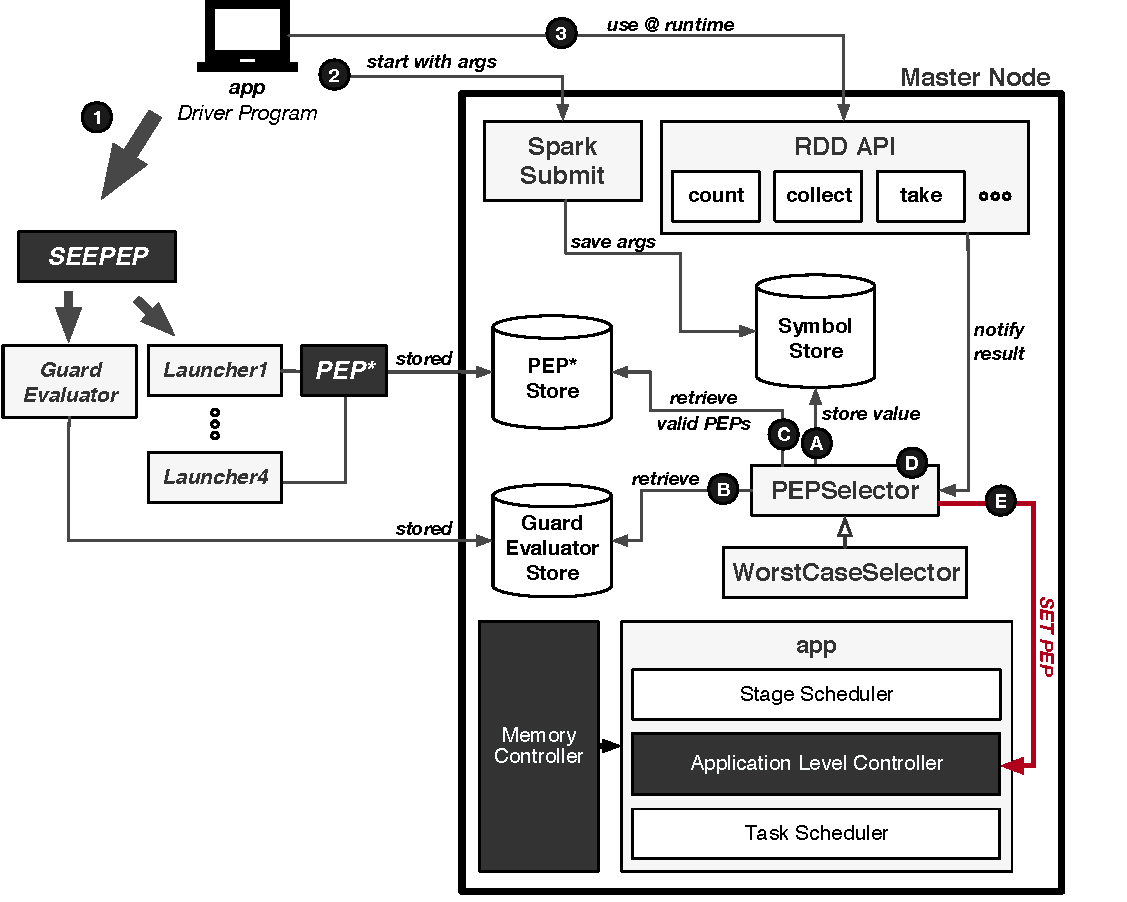
\includegraphics[width=\columnwidth]{images/xsparksymb}
	\caption{\tool}
	\label{fig:xsparkdagsymb}
\end{figure}

Figure~\ref{fig:xsparkdagsymb} shows the main elements of the tool-chain and exemplifies it on profiling and controlling the example application of Figure~\ref{fig:xdag2} ---\textit{app}, hereafter. As first step, \dSymb generates the $4$ ($n$, in general) launchers, which activate the four ($n$) \plans of the program, and an application specific \textit{GuardEvaluator}. 

The new toolchain associates each \plan to its path condition, it uses the generated launchers to obtain the profiling data of each \plan and synthesize the \model for the application that is then stored in the master node in component \textit{PEP* Store}. Finally the generated \textit{GuardEvaluator}, which implements a common interface to be dynamically instantiated and used without a static import in the source code of \cSpark, is also stored in the master node (component \textit{GuardEvaluator Store}).

After this phase, $app$ can be executed and controlled by \cSpark. 
Since the application parameters can be part of a path condition as symbols, we modified component \textit{SparkSubmit} to store their values. A symbol is identified by application name, action name, code line in the driver program, and a counter to take multiple executions into account  (i.e., loops or recursive functions). 

At runtime, everytime an action is executed, that is, a result is computed and returned to the driver program, our modified version of the  \textit{RDD API} notifies component \textit{PEPSelector} that a new result is available. This component is in charge of selecting the \plan and its profiling data then used by \textit{Application Level Controller} to compute the local deadlines for the next stages and thus to provision resources. \textit{PEPSelector} saves computed results into component \textit{Symbol Store}, retrieves an instance of the dedicated \textit{GuardEvaluator}, and feeds it with all the symbols resolved 
by the aforementioned results. \textit{GuardEvaluator} returns the list of \plan whose path conditions still hold.

This means, for example, that at the beginning of the execution of function \textit{run} of $app$, four \plans are valid since neither $x$ nor $y$ have been resolved to a value. The job at line $4$ produces the value of $x$ and if the value is less than or equal to $threshold$,  the if statement of line $8$ is not evaluated. Therefore, even if the value of $y$ is still unknown, \textit{GuardEvaluator} only returns two \plans, that is, the only two \plans whose path conditions still hold: it excludes all the path conditions that depends on the expression $x > threshold$). This way, since the \plan is updated constantly, \cSpark becomes aware of what has been actually done, and can use this information to refine resource provisioning.  

Note that \textit{PEPSelector} receives all the valid \plans and computes the next \plan to use. This selection can be customized by the user. Currently, we always select the worst-case \plan, that is, the \plan with the greatest number of remaining stages to be conservative and minimize deadline violations. If one wanted to optimize different performance indicators (e.g., deadlines are not strict and used resources must be minimized), the selection could privilege a \plan that corresponds to an average case instead of the worst one. 
	\chapter{Implementation} \label{chap:implementation}
\begin{flushright}{\slshape    
   Science, my boy, is made up of mistakes, but they are mistakes
   which it is useful to make, because they lead little by little
   to the truth}. \\ \medskip --- \citeauthor{verne_journey:1957}
   \citetitle{verne_journey:1957} \citeyear{verne_journey:1957}
\end{flushright} 

\lettrine[lines=4]{\textcolor{purple}{I}}{n} this chapter we show the implementation details of \tool, which consists of the modifications to existing xSpark component, new components added to xSpark, \textit\approach\xspace concrete application \textit {launchers} and the {xSpark-dagsymb} python tool that was used to launch the experiments to generate the data for the evaluation of the solution.

%\begin{itemize}
%	\item Modifications to existing xSpark components
%	\item New components added to xSpark
%	\item \textit\approach\xspace concrete application \textit {launchers}
%	\item \textit {xSpark-dagsymb} python tool
%\end{itemize}

\section{Overview}\label{sec:impl_overview}
\MyFig{fig:solution_impl_overview} shows a simplified overview of the components of the solution. New components are highlighted with a yellow dotted-pattern background, modified components are are highlighted with a grey background.
\begin{figure}[tbhp]
	%\hspace*{-2cm}
	\centering
	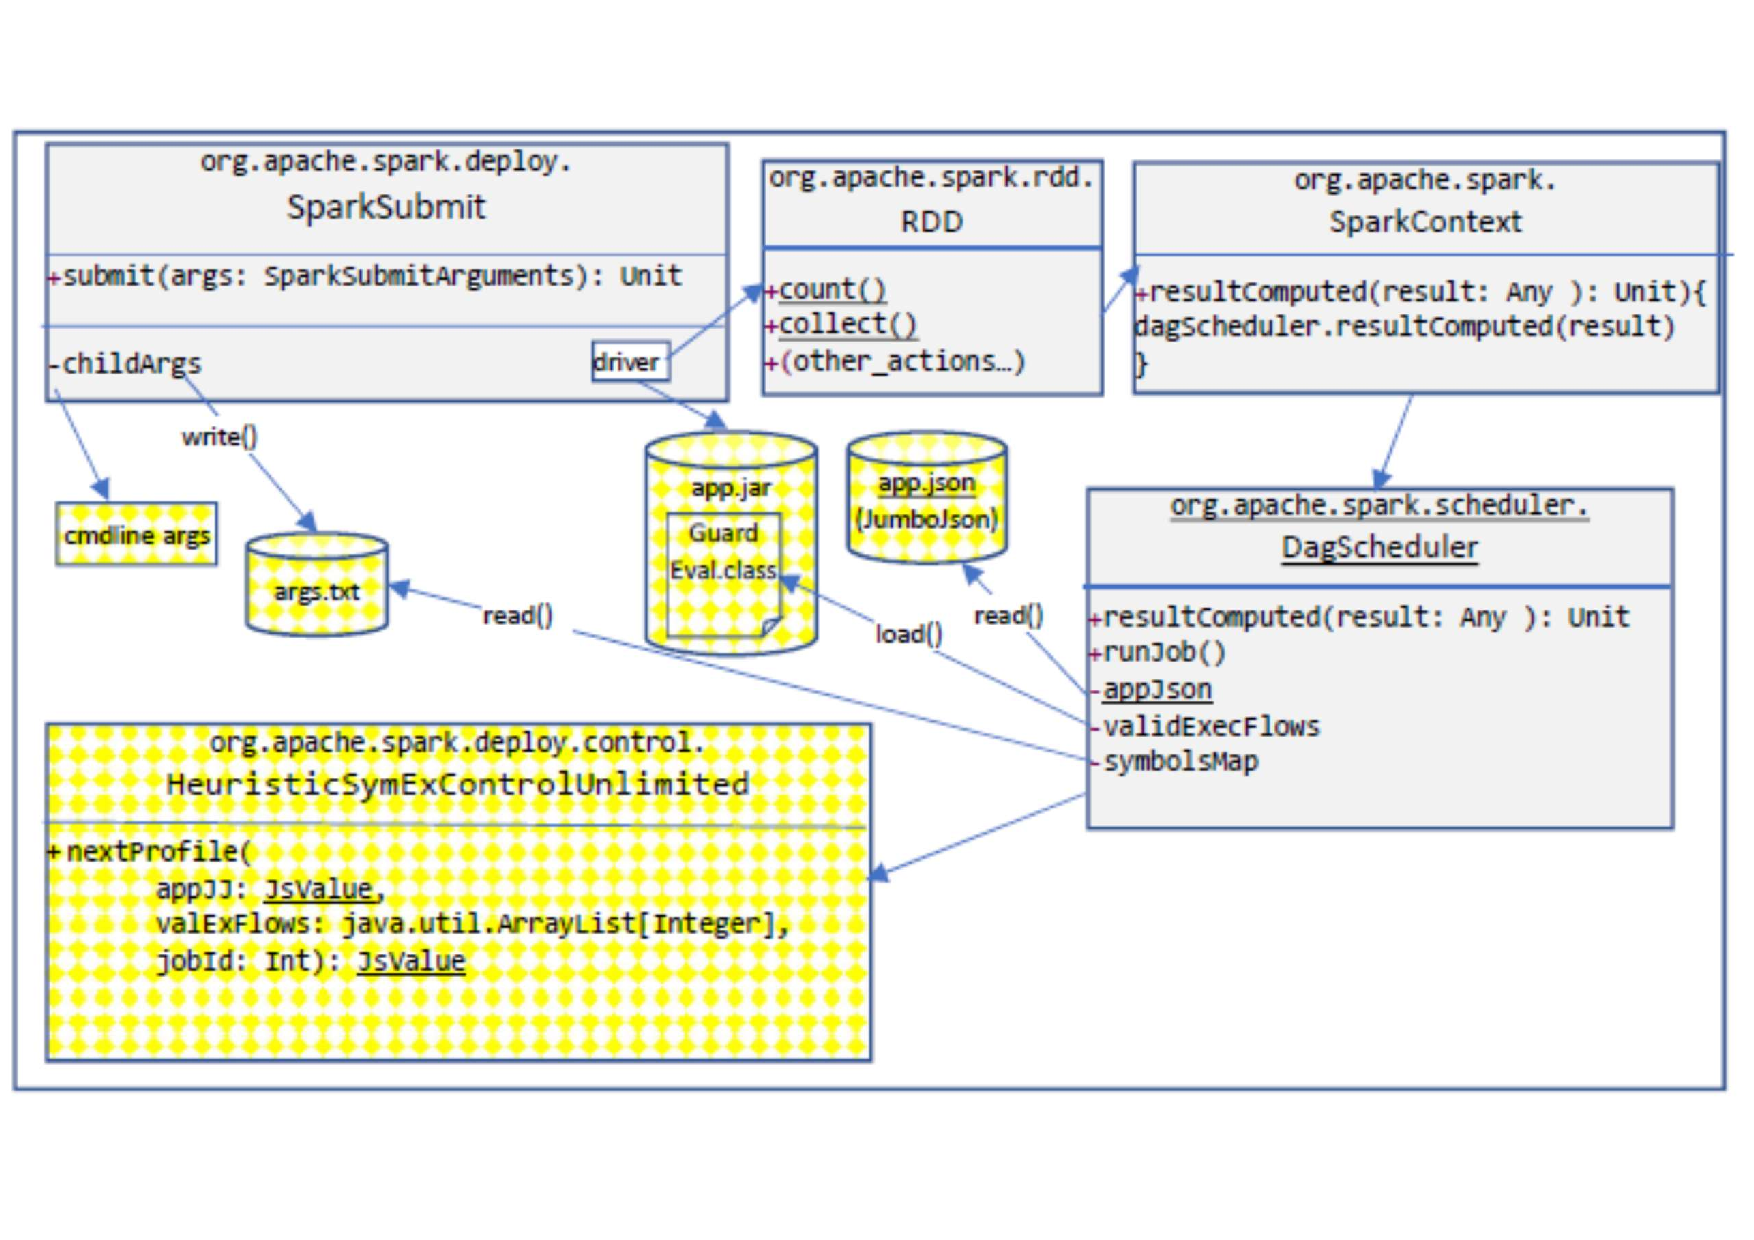
\includegraphics[width=12cm]{images/solution_impl_overview}
	\caption{Simplified solution components overview.}
	\label{fig:solution_impl_overview}
\end{figure}


\subsection{Background: Current xSpark Heuristic}\label{sec:impl_background}
%We recap here the information given in \MySec{sec:heuristic}.

xSpark uses a heuristic to compute per-stage deadlines and to estimate how many cores must be allocated for a stage to successfully fulfill the deadline. See \MySec{sec:heuristic} for an exhaustive description of its funcionality.
%At submission time three parameters: are collected: i) the application deadline, ii) the cluster size, and iii) the number of cores per worker node. Before executing the application, xSpark performs a feasibility check given the available resources. When a stage is submitted for execution, its deadline is computed \[deadline(sk) = \dfrac{\alpha\cdot ApplicationDeadline - SpentTime}{weight(sk)}\] where $SpentTime$ is the time already spent for execution and $\alpha$ a value between 0 and 1 that xSpark uses to be more conservative with respect to the provided ApplicationDeadline. The weight is computed 
%\[\begin{cases}
%w1(sk) = \#(RemainingStages + 1)\\
%w2(sk) = \dfrac{{\Sigma}_{{a}_{i=k}}^{k+{w}_{1}}duration(s_i)}{duration(sk)}\\
%weight(sk) = \beta\cdot w1(sk) + (1 - \beta) \cdot w2(sk)\\
%\end{cases}\]
%where w1 is the number of stages still to be scheduled (s included) and w2 is the rate between the duration of s and the duration of the remaining stages (s included). xSpark then proceeds to estimate how many cores are needed to execute the stage:
%\[estimatedCores(sk) = \lceil {\dfrac {inputRecords(sk)}{deadline(sk) \cdot nominalRate(sk)}}\rceil\]
%where inputRecords is the number of records that will be processed by sk and nominalRate is the number of records processed by a single core per second in stage sk.

%Since xSpark controls the resource allocation of a stage before and during the execution, the maximum amount of allocable cores needs to be greater than the estimated one, in order to be able to accelerate when progressing slower than expected 
%\[maxAllocableCores(sk) = overscale \cdot estimatedCores(sk)\]
%The final step determines the initial number of cores that should be assigned to the different executors. xSpark distributes the cores equally among the available workers by creating one executor per stage per worker. In this way, it is guaranteed that executor performances will be the same for each of them, and that xSpark can compute the same deadline for all the executors. The initial number of cores per executor is computed as
%\[initCorePerExec(sk) = \lceil\dfrac {maxAllocableCores(sk)}{overscale \cdot cq \cdot numExecutors}\rceil\cdot cq\]
%where $numExecutors$ is the number of executors and $cq$ is the $core\quantum$, a constant that defines the quantization applied to resource allocation, the smaller this value is, the more precise the allocation.

\subsection{Current xSpark Scheduling Limitation}\label{sec:impl_xspark_sched_limitation}
At runtime, an annotated DAG allows the xSpark scheduler function to comprehend how much work has already been completed and how much work still needs to be done. This means that xSpark can only optimize the allocation of the resources if the execution of all jobs of the application use the same DAG. This might not always be the case, for example when the code contains branches or loops, because these might need to be resolved in different ways at runtime. This is a severe limitation of the xSpark capability to manage real-world applications.

\section{Implementation Scope and Objective}\label{sec:impl_scope_objective}
The current work, by addressing the xSpark limitation explained above, aims at extending the scope of applicability of xSpark enhancing it with the capability to manage the case of applications that can potentially generate, at runtime, a different DAG at each execution. The code in this kind of applications includes conditional branches or iterative loops whose outcomes can only be resolved at runtime because they depend on user input values or results from previous computations that cannot be predicted or folded to constant values by the compiler. 
\subsection{Symbolic Execution}\label{sec:impl_symbolic_execution}
Executing a program symbolically means to simultaneously explore multiple paths that a program could take under different inputs. The key idea is to allow a program to take on symbolic – rather than concrete – input values. Execution is performed by a symbolic execution engine, which maintains for each explored control flow path: 
(i)	a first-order Boolean formula that describes the conditions satisfied by the branches taken along that path, and (ii) a symbolic memory store that maps variables to symbolic expressions or values. 

When a conditional branch is met, both sides of the branch are executed. Branch execution updates the formula, while assignments update the symbolic store. 
A symbolic execution tree is generated with an execution state associated with each node, containing the statement to be executed, the symbolic store, and the path conditions (a formula that expresses a set of assumptions on the symbols). The leaves of the tree identify the end of the computations, and tracing back from each leaf up to the root of the tree allows us to reconstruct, in reverse order, all the possible execution paths of the program. Our implementation exploits the funcionality provided by  \textit{GuardEvaluator}, an extension to Spark applications explained in \MySec{sec:guard_evaluator}, which is generated by an external implementation of the ligthweight symbolic execution algorithm  described in \MySec{sec:lightweight_symbolic_execution}.

\subsection{\tool vs. xSpark}
The first important difference between \tool and xSpark is in the profiling of the applications. xSpark requires the generation of a single DAG profile per application, while \tool requires a family of DAG profiles, one for each possible execution path, each of them associated to a unique set of “Path Conditions”. Profile information is collected in special JSON files, called "JSON profiles". \MyListing{lst:profile_example} shows an example of a JSON profile.
\lstinputlisting[
firstline=1,
lastline=141,
%float=thb,
language=python,
tabsize=2,
numbers=left,
numberstyle=\tiny,
stepnumber=1,
numbersep=5pt,
caption={Example of JSON profile.}, 
captionpos=t,
label=lst:profile_example
]{CodeFiles/CallsExample-1.json}

The profiling information for a \tool application is obtained by combining the JSON profiles, obtained by driving the application with different sets of input data so to drive the execution of all the possible execution paths, into a JSON file that we will call with a jargon “JumboJSON”, as shown in \MyFig{fig:jumboJSON_structure}.
\begin{figure}[tbhp]
	\hspace*{-2cm}
	\centering
	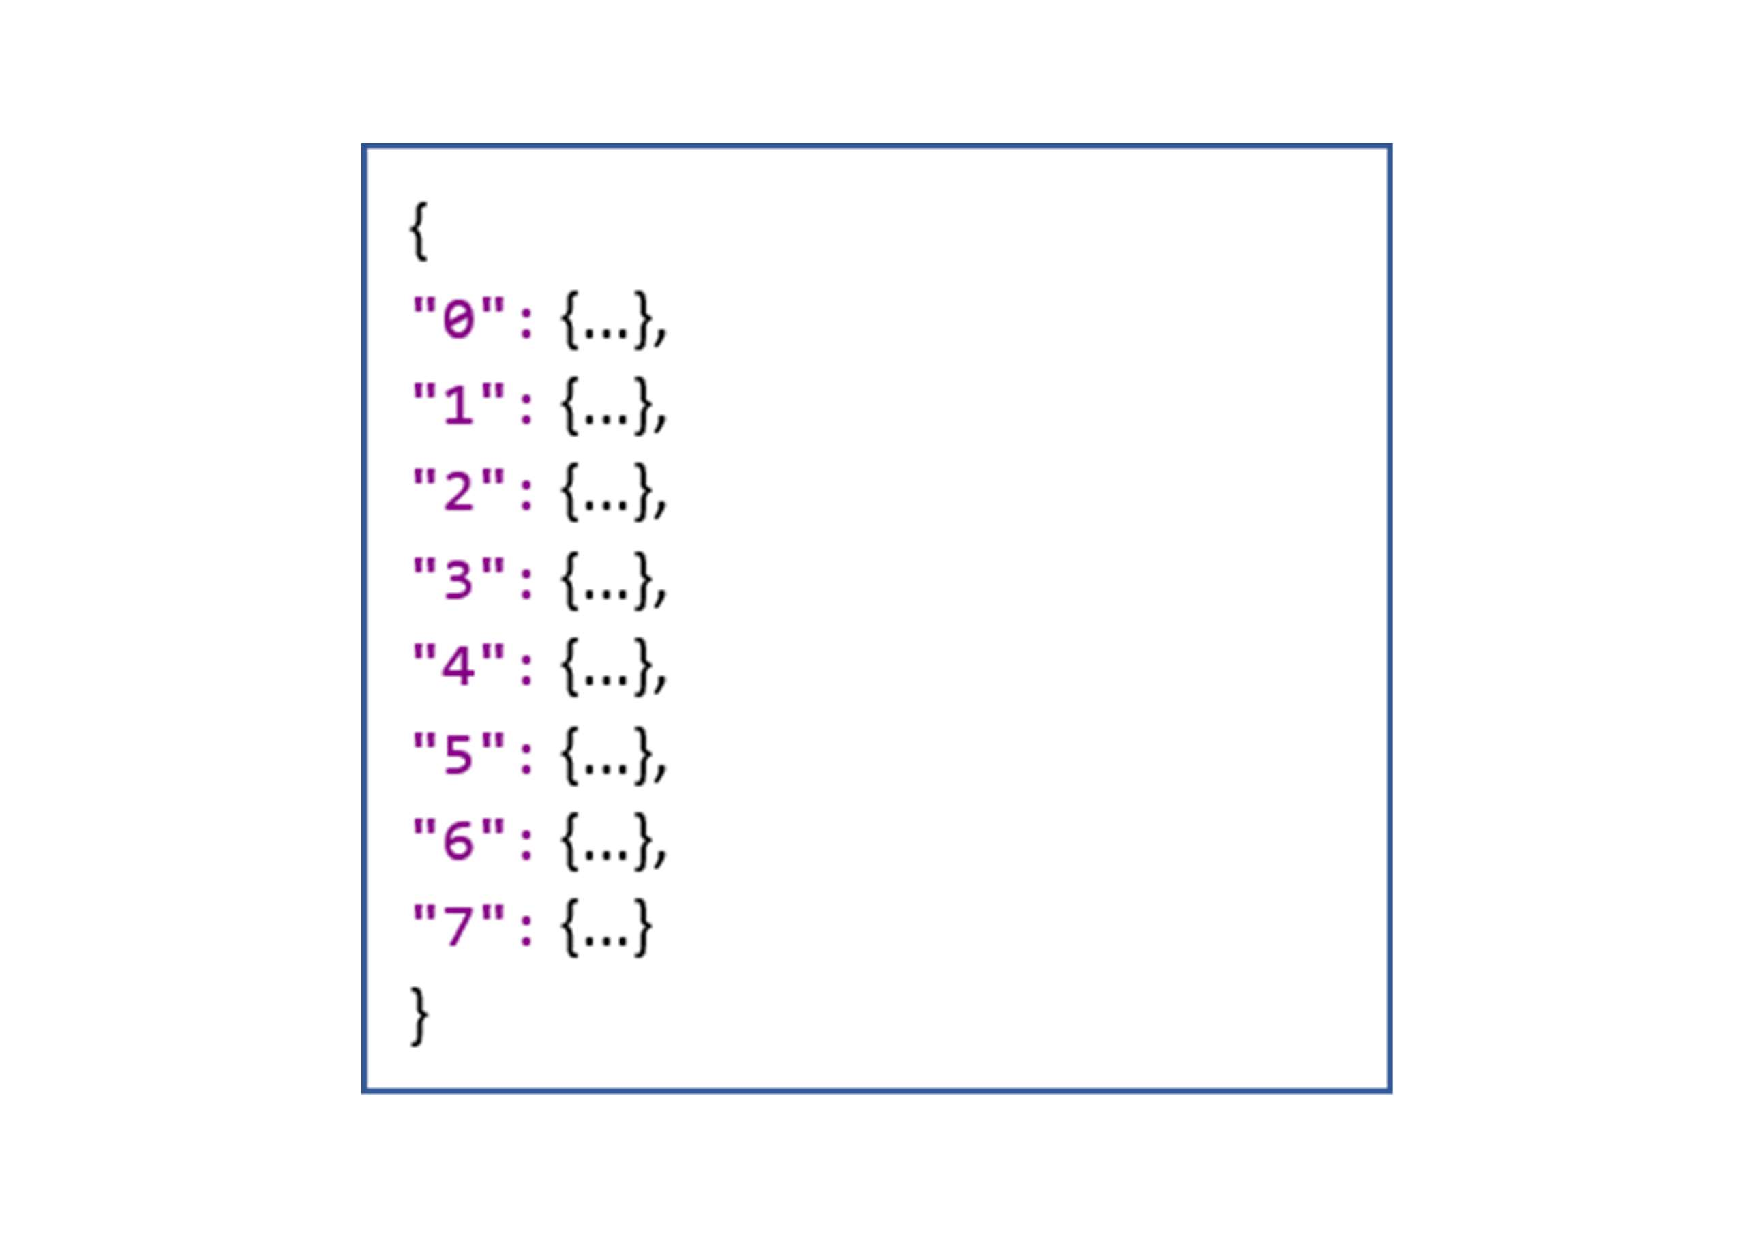
\includegraphics[width=18cm]{images/xsparksymb_profile_structure}
	\caption{Structure of profile JumboJSON. Each profile is identified by its profile id's {"$0$", "$1$", ...,"$7$"} and, in general, is characterized by its own number of stages and key values. Left and right images show the same JumboJSON profile where profile "$0$" (left) and profile "$1$" (right) are expanded, to show their difference in terms of number of stages ($6$ stages for profile $0$ and $3$ for profile $1$ ) and totalduration ($76,200$ ms for profile $0$ ms and  $43,000$ ms for profile $1$).}
	\label{fig:jumboJSON_structure}
\end{figure}
Futhermore, each single json profile is enhanced with information about the jobs composing the application, as shown in \MyFig{fig:profile_jobs_info}. 
\begin{figure}[tbhp]
	%\vspace*{-1cm}
	\hspace*{-1.7cm}
	\centering
	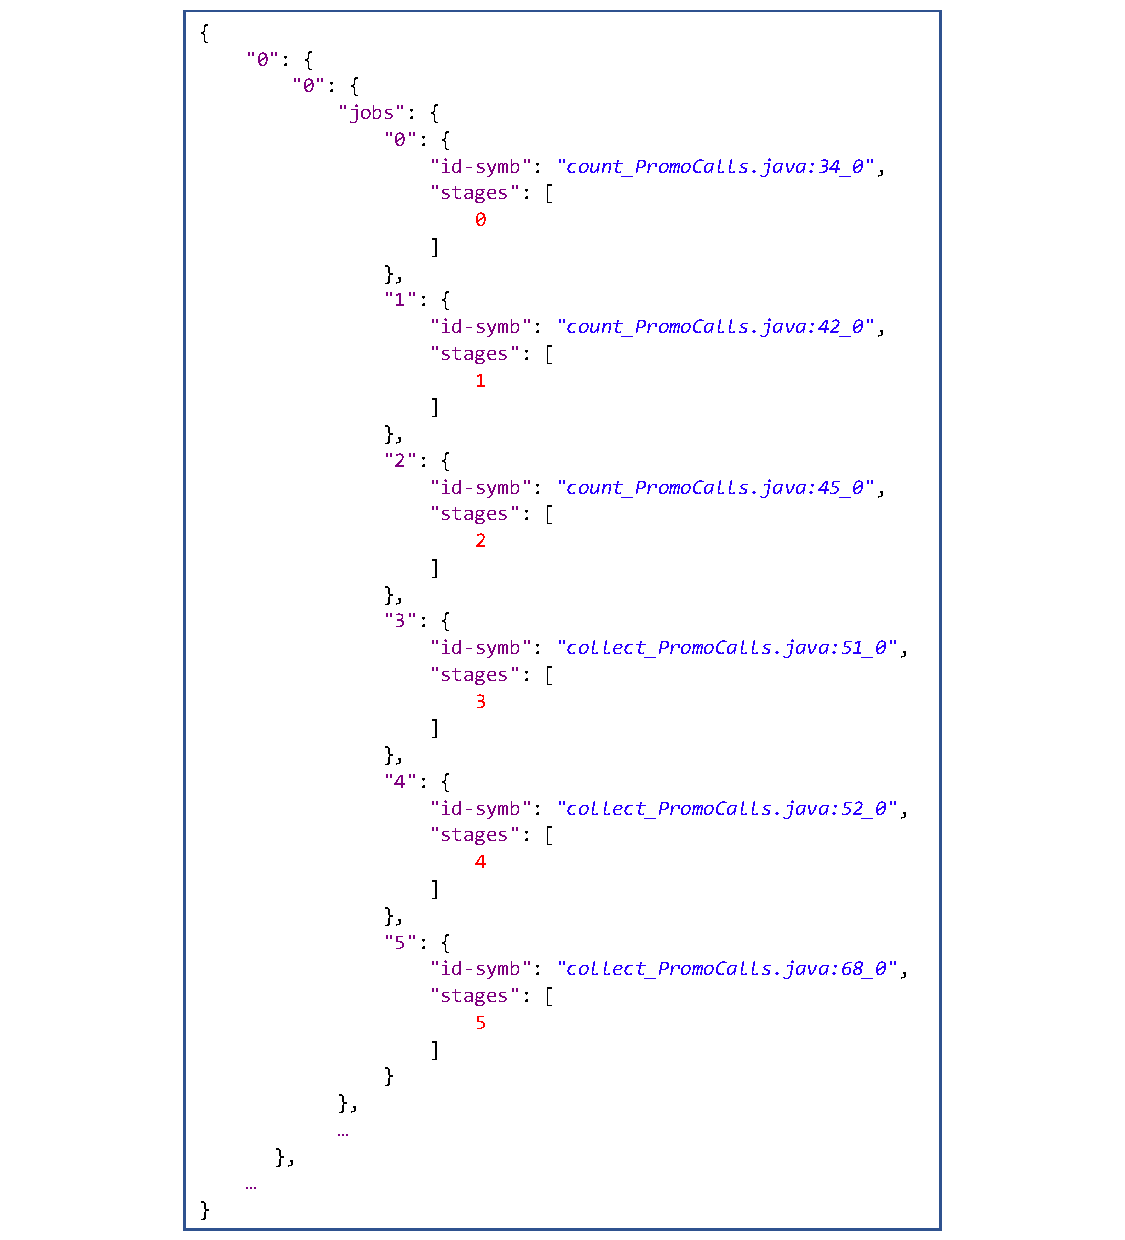
\includegraphics[width=15cm]{images/xsparksymb_profile_jobs_info}
	\caption{Information about jobs in json DAG profile.}
	\label{fig:profile_jobs_info}
\end{figure}
Inside \tool is kept a symbolic memory store that maps symbolic values (or symbols) to actual values. To this structure, initially empty, a new entry is added every time a symbolic value gets assigned a concrete value. Each entry is a key-value pair containing the symbol as key and the assigned value as value. The convention adopted for naming the symbols is the following:
\begin{itemize}
	\item \textbf{Commandline arguments}: prefix “arg\_” followed by an integer reflecting the position of the argument on the commandline. For example: “arg\_0”, “arg\_1” etc…
	\item \textbf{Program variables}: Spark action name followed by “\_”, followed by program name followed by “:”, followed by the program line number where the action is called, followed by “\_”, followed by an integer representing the number of times the action in the same line of code is being repeated. For example: "count\_PromoCalls.java:34\_2"
\end{itemize} 
\begin{table}[tbhp]
	\centering
	\caption{Example of Symbolic Memory Store contents.}
	\label{Table:impl_symbolic_memory_store_contents}
	\begin{tabular}{|c|c|c|}
		\hline
		\textbf{Entry\#} & \textbf{Key} & \textbf{Value} \\ \hline
		0	& arg\_0						&  100      \\ \hline
		1	& arg\_1						&  200      \\ \hline
		2	& arg\_2						&  300      \\ \hline
		3	& count\_PromoCalls.java:42\_0	& 2350      \\ \hline
		4	& count\_PromoCalls.java:45\_0	& 1920      \\ \hline
		5	& count\_PromoCalls.java:45\_1	& 3800      \\ \hline
	\end{tabular}
\end{table}
\MyTab{Table:impl_symbolic_memory_store_contents} shows an example of symbolic memory store contents during the execution of the application, run with three commandline arguments having value “100”, “200”, “300” and two spark actions already executed, of which the second was executed twice.
The application is also required to provide a class implementing a method called \texttt{evaluateGuards} that receives in input a Map of a symbolic memory store (as the one described above) and returns a list of the profile id’s whose DAG’s are still executable (i.e. they contain execution paths whose Path Conditions are satisfiable).

\subsection{A new Heuristic}\label{sec:new_heuristic}
\tool implements \texttt{HeuristicSymExControlUnlimited}, a 
new heuristic that extends \texttt{HeuristicControlUnlimited}. 
%\MyFig{fig:heuristic_simplified_class_diagram} below shows the simplified class diagram showing the relationships between the heuristic classes in the spark.deploy.control package.
The class diagram with the relationships between the heuristic classes is shown in \MyFig{fig:heuristic_class_diagram}. A new method, \texttt{nextProfile}, is implemented by the new heuristic. It takes the following input parameters:
\begin{enumerate}[$1) $] 
	\item a json containing the application profiles obtained by the concrete execution of every possible execution path of the application;
	\item a list of the profile id’s that are still satisfiable;
	\item the id of the job being submitted;
\end{enumerate}
and returns the json of the application profile to be used during the execution of the next job.
%\begin{figure}[tbhp]
%	\vspace*{-1cm}
%	\hspace*{-3cm}
%	\centering
%	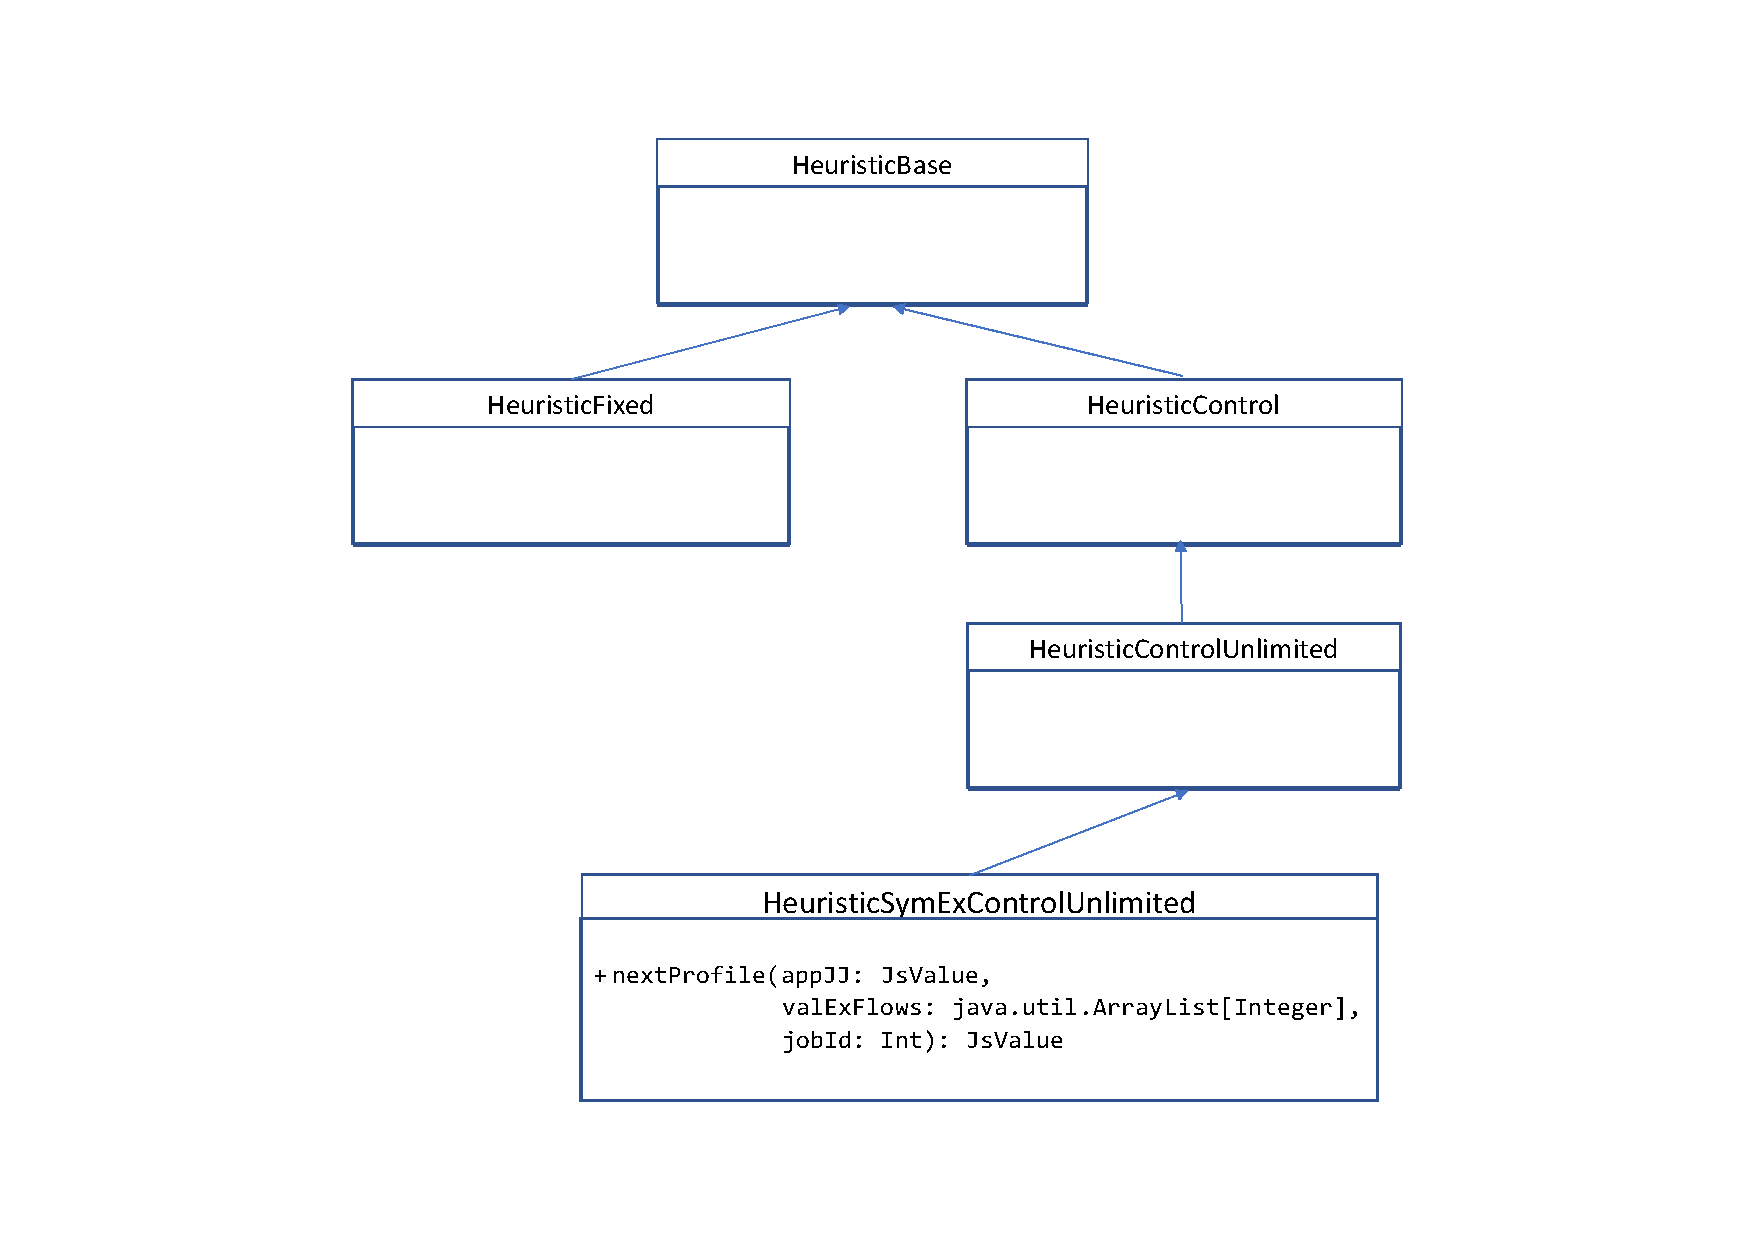
\includegraphics[width=16cm]{images/heuristic_simplified_class_diagram}
%	\vspace*{-1cm}
%	\caption{\tool Heuristic related simplified class diagram.}
%	\label{fig:heuristic_simplified_class_diagram}
%\end{figure}
Keeping in mind that the scheduler uses the \texttt{HeuristicSymExControlUnlimited} to estimate how many cores are needed to execute the stage, given the application deadline and the parameters in the application profile, we expect the new heuristic to choose the profile so as not to jeopardize the controller's ability to meet the deadline. This can be achieved by choosing a profile that will lead to not underestimate the cores needed to execute the remaining stages. All the following parameters seem to be good proxies for estimating the remaining computing effort:
\begin{verbatim}
1)	Number of remaining stages to be executed
2)	Sum of duration of remaining stages to be executed
3)	Weighted combination of 1 and 2 above
\end{verbatim}
The above parameters can be calculated using the data inside the application json profile. 
Current implementation of the heuristic uses proxy \#1 (number of remaining stages to be executed). It calculates the value for each of the satisfiable profiles, and then selects the profile associated to the maximum value of the proxy. This way, we supply the “worst case” profile to the heuristic, so that the stage deadline is not overestimated and consequently the number of cores to be assigned for the next stage execution is not underestimated.

\section{Application Parameters}\label{sec:application_parameters}
As explained in ~\MyChap{chap:ProblemAndSolution}, the application parameters can be part of a path condition as they could have been associated to a symbol by the symbolic executor part of \dSymb. Hence, we have introduced in xSpark a mechanism to intercept and store these application parameters in the \tool \textit{Symbol Store}, as shown in \MyFig{fig:xsparkdagsymb}.  \MyListing{lst:SparkSubmit_submit} shows part of the code of method \textit{submit} of xSpark class \textit{SparkSubmit}, that was modified in order to read the values of the application's runtime arguments passed via the Spark \textit{submit} command and write them as separate lines to textfile \textit{args.txt}. This file is a component of the \textit{\model Store}. Records from this file are read by xSpark at a later stage, when lazily executing the application by means of job scheduling.
 
\lstinputlisting[
firstline=1,
lastline=13,
%float=thb,
language=scala,
tabsize=2,
numbers=left,
numberstyle=\tiny,
stepnumber=1,
numbersep=5pt,
caption={Changes to SparkSubmit method "submit".}, 
captionpos=t,
label=lst:SparkSubmit_submit
]{CodeFiles/SparkSubmit_submit.scala}

\section{Application Profiling}\label{sec:application_profiling}
As shown in \MyFig{fig:xsparkdagsymb}, for each set of input parameters identified by \dSymb a \textit{Launcher} is generated. A \textit{Launcher} is a Java class which contains the command to run the application with a specific set of arguments, which is in a 1:1 relationship with the application parameters of the corresponding \plan. An example of Launcher class is shown in \MyListing{lst:LauncherExample}. 

A \textit{Profiling} (see \MyFig{fig:xSparkExecFlow}
) of the application is done by running it with each \textit{Launcher}'s set of arguments. Each profiling run generates the corresponding \plan in a specialized JSON file. At the end of this process, all the generated \plans are packaged into another JSON file, in jargon called \textit{JumboJSON}, to form the \model. All the generated JSON files are then stored along with the \model \textit{Store} on the \textit{Spark Master} server. 
\lstinputlisting[
firstline=1,
lastline=42,
%float=thb,
language=java,
tabsize=2,
numbers=left,
numberstyle=\tiny,
stepnumber=1,
numbersep=5pt,
caption={Example of Launcher Code .}, 
captionpos=t,
label=lst:LauncherExample
]{CodeFiles/Launcher0.java}


\section{PEP*}\label{sec:getting_peps}
The previous version of xSpark required a single \plan to be present in the \textit{\plan Store}, so we had to modify the xSpark class \textit{DAGScheduler} to  account for the data in the \textit{JumboJSON file} that now contains all the \plans. To maintain backwards compatibility, a new variable was introduced, \texttt{JumboJson}, to hold the contents of the \model Store. The modified code is in charge of checking the \textit{heuristic type} in the \textit{SparkContext} instance \texttt{sc}, to understand if it should expect the contents of the \model Store to be a single \plan or a whole set of \plans representing a \model. The heuristic type is initialized with the value of the key \textit{spark.control.heuristic} specified in the xSpark configuration file \textit{spark-defaults.conf}. 

\lstinputlisting[
firstline=1,
lastline=10,
%float=thb,
language=scala,
tabsize=2,
numbers=left,
numberstyle=\tiny,
stepnumber=1,
numbersep=5pt,
caption={Changes to class DAGScheduler.scala - reading PEPs.}, 
captionpos=t,
label=lst:DAGScheduler-profile
]{CodeFiles/DAGScheduler_profile.scala}

\section{GuardEvaluator}\label{sec:guard_evaluator}
With the term \textit{GuardEvaluator} we collectively refer to the interface class \texttt{IGuardEvaluator} and its implementation class defining the \texttt{evaluateGuards} method, that is in charge of returning the list of valid profiles (\plans) when it is called with the HashMap of the known symbols and their values. The code of the  \texttt{IGuardEvaluator} interface is shown in \MyListing{lst:IGuardEvaluator}, while \MyListing{lst:GuardEvaluatorPromoCallsFile} shows an example of an implementation class and its method \texttt{evaluateGuards} for a specific application.
\lstinputlisting[
firstline=1,
lastline=9,
%float=thb,
language=java,
tabsize=2,
numbers=left,
numberstyle=\tiny,
stepnumber=1,
numbersep=5pt,
caption={Interface class IGuardEvaluator.}, 
captionpos=t,
label=lst:IGuardEvaluator
]{CodeFiles/IGuardEvaluator.java}
\lstinputlisting[
firstline=1,
lastline=142,
%float=thb,
language=java,
tabsize=2,
numbers=left,
numberstyle=\tiny,
stepnumber=1,
numbersep=5pt,
caption={Class GuardEvaluatorPromoCallsFile, implementing the IGuardEvaluator interface.}, 
captionpos=t,
label=lst:GuardEvaluatorPromoCallsFile
]{CodeFiles/GuardEvaluatorPromoCallsFile.java}


The application is in charge of providing the \textit{GuardEvaluator} as a java class, implementing the interface \texttt{IGuardEvaluator}, and packaged inside the jar of the application. This class is loaded dynamically at runtime by the new code added for this purpose to the xSpark class \texttt{DAGScheduler} and shown in \MyListing{lst:DAGScheduler_GuardEvaluator}.
\lstinputlisting[
firstline=1,
lastline=22,
%float=thb,
language=scala,
tabsize=2,
numbers=left,
numberstyle=\tiny,
stepnumber=1,
numbersep=5pt,
caption={Changes to class DAGScheduler.scala - Loading GuardEvaluator.}, 
captionpos=t,
label=lst:DAGScheduler_GuardEvaluator
]{CodeFiles/DAGScheduler_GuardEvaluator.scala}

\section{Symbol Store}\label{sec:symbol_store}
In order to take advantage of the symbolic execution, we need to maintain an updated   \textit{Symbol Store} containing all the symbols that can be part of a path condition and their associated determinations (assigned values). We added the code into the xSpark class \texttt{DAGScheduler} to abstractely represent the \textit{Symbol Store} as a  \textit{HashMap[String, Any]}. Each entry of this HashMap stores a \textit{known symbol} name and its value. By \textit{known symbol} we mean a symbol that has been associated to a value during the concrete execution of program code. Given this defintion, at the very beginning of the computation the only known symbols are the runtime arguments passed to the application. We added to the xSpark class \texttt{DAGScheduler} the code to read the arguments and their values and create the corresponding \textit{Symbol Store} entries. The code is shown in \MyListing{lst:DAGScheduler_symbol_store}, where we can notice that the first two arguments loaded when var \textit{iter} is set to negative values ($-2\ and -1$) are respectively the \textit{GuardEvaluator} class name and the application jar name, that are not symbols. They are not kept in the Symbol Store, instead they are used to initialize the variables \texttt{guardEvalClassname} and \texttt{appJar} which will be needed in a later step of the execution to identify the location and dynamically load the class implementing the \textit{GuardEvaluator} function.
\lstinputlisting[
firstline=1,
lastline=17,
%float=thb,
language=scala,
tabsize=2,
numbers=left,
numberstyle=\tiny,
stepnumber=1,
numbersep=5pt,
caption={Changes to class DAGScheduler.scala - Initializing Symbol Store.}, 
captionpos=t,
label=lst:DAGScheduler_symbol_store
]{CodeFiles/DAGScheduler_symbol_store.scala}
\section{Heuristic}\label{sec:impl_heuristic}
The heuristic used by xSpark is determined by the value of configuration parameter spark.control.heuristic and is an implementation of the class \texttt{HeuristicBase}, whose class diagram is shown in \MyFig{fig:heuristic_class_diagram}. In  \MyListing{lst:ControlEventListener_heuristic}, we can see that the heuristic \textit{HeuristicControl} is used by default, but other heuristics can be selected. \texttt{HeuristicFixed} and \texttt{HeuristicControlUnlimited} were already available in xSpark, while we implemented a new heuristic  \textbf{\texttt{HeuristicSymExControlUnlimited}} to exploit \textit{Symbolic Execution}.
\lstinputlisting[
firstline=1,
lastline=13,
%float=thb,
language=scala,
tabsize=2,
numbers=left,
numberstyle=\tiny,
stepnumber=1,
numbersep=5pt,
caption={Changes to class ControlEventListener.scala - selecting the heuristic.}, 
captionpos=t,
label=lst:ControlEventListener_heuristic
]{CodeFiles/ControlEventListener_heuristic.scala}
\begin{figure}[tbhp]
	\hspace*{-4cm}
	\centering
	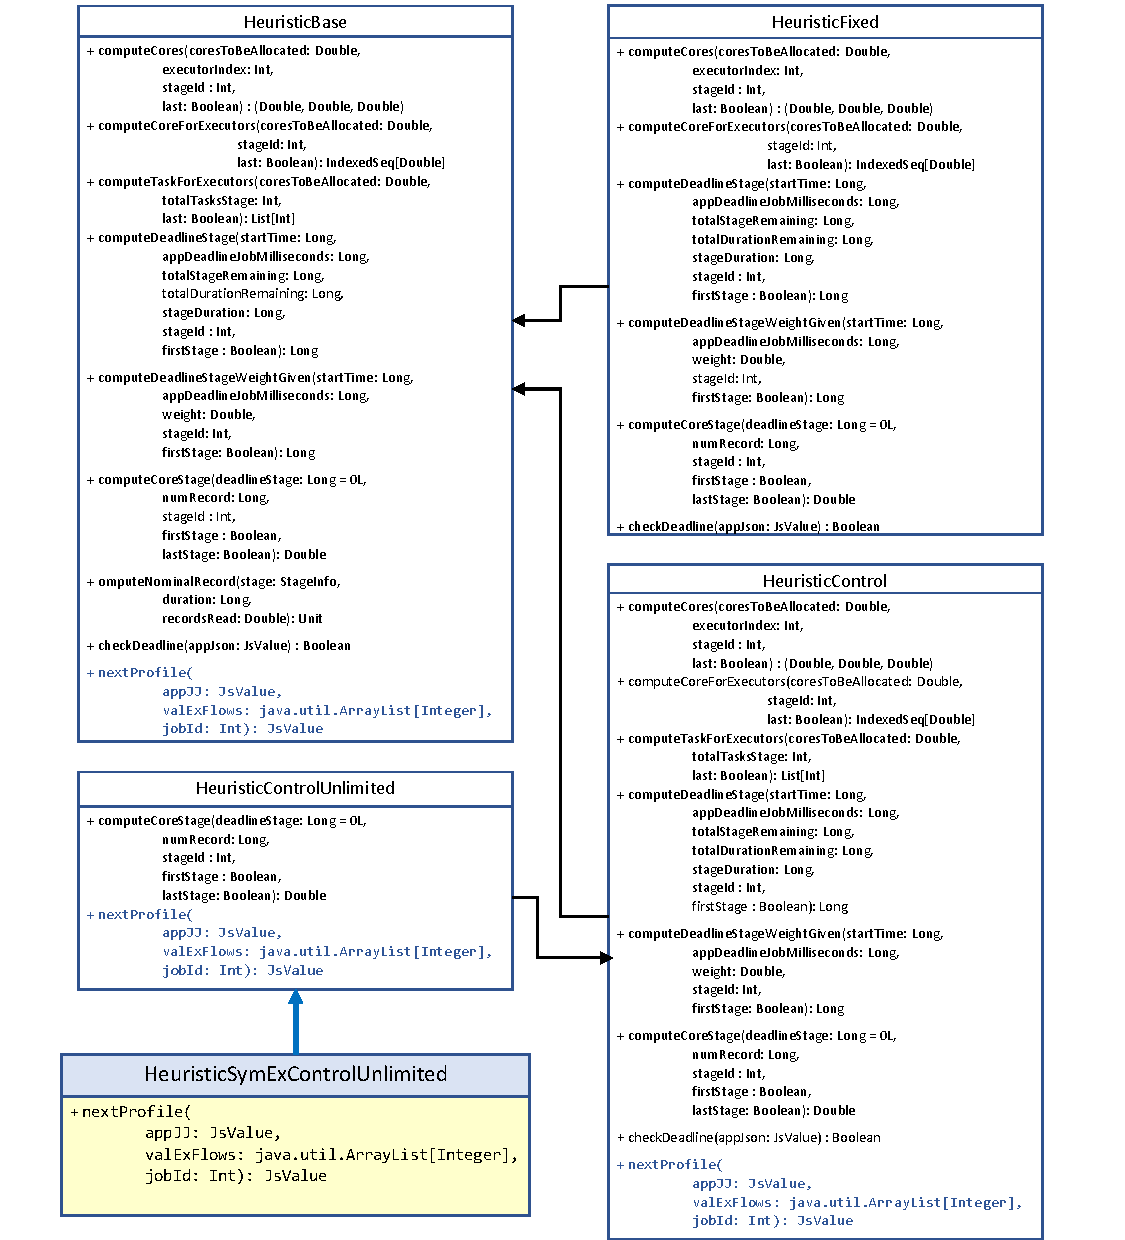
\includegraphics[width=20cm]{images/heuristic_class_diagram}
	\caption{Class diagram of Heuristic related classes.}
	\label{fig:heuristic_class_diagram}
\end{figure}
\texttt{HeuristicSymExControlUnlimited} extends \texttt{HeuristicControlUnlimited} by adding the implementation of a new method, \texttt{nextProfile}, taking parameters \texttt{appJson}, the \texttt{JumboJSON} containing the \model representation and \texttt{valExFlows}, a list containing the id's of the valid application profiles,(i.e. the list of the \plans whose path conditions still hold true), and returns the \plan of the profile to be used during the executing of the next scheduled job.
\lstinputlisting[
firstline=1,
lastline=27,
%float=thb,
language=scala,
tabsize=2,
numbers=left,
numberstyle=\tiny,
stepnumber=1,
numbersep=5pt,
caption={Class HeuristicSymExControlUnlimited.scala implementation.}, 
captionpos=t,
label=lst:HeuristicSymExControlUnlimited
]{CodeFiles/HeuristicSymExControlUnlimited.scala}
Class \texttt{HeuristicSymExControlUnlimited} implementation code is shown in \MyListing{lst:HeuristicSymExControlUnlimited}. The \plan selection is made by choosing the \textit{"worst case"} among the valid \plans, that is the \plan with the maximum number of stages still to be executed, as we want to be conservative and minimize the deadline violations. If we wanted to optimize another performance indicator, like minimum  resource utilization in absence of strict deadline commitment, we could choose the profile with an average number of remaining stages to be executed. 
  
\section{Symbols}\label{sec:symbols}
As mentioned in \MySec{sec:symbol_store}, we have to update the Symbol Store everytime a variable associated to a symbol is evaluated by the concrete execution of the application. We adopted the convention to identify a symbol by the string \textit{arg\_n} if it refers to a runtime application argument, where n is the position of the argument (e.g. \textit{arg\_$0$}), or by a string obtained by concatenating its \textit{CallSite} and \textit{IterationNumber} separated by an underscore character \textit{"\_"}, where \textit{Call Site} is a string obtained by concatenating \textit{SparkActionName}, \textit{ApplicationClassName}, \textit{SourceLanguageName:SourceLineNumber} separated by an underscore character \textit{"\_"}, and  \textit{IterationNumber} is an integer starting from $0$ and incremented everytime a call is originated by the same \textit{CallSite}. i.e. the same line of code is re-executed (e.g. due to iterative loops). Examples of formal symbol names are shown in \MyFig{fig:symbol_name}.
\begin{figure}[tbhp]
	\centering
	\begin{lstlisting}[basicstyle=\ttfamily\scriptsize]
		          arg_0
		          count_PromoCalls_java:45_2
	\end{lstlisting}
	\caption{Example of symbol formal names.}
	\label{fig:symbol_name}
\end{figure}

As stated above, a symbol, if not associated to an application runtime argument,  is identified by its \textit{CallSite}. This means that to identify the symbols we have to intercept calls coming from their  \textit{CallSite}. Since the values associated to a symbol can only be changed by xSpark \textit{actions} which delimit jobs, we added code to the method \texttt{runJob} of class \texttt{DAGScheduler} to extract the \textit{CallSite}, generate a symbol and push it in the \textit{Symbol Store} everytime the method \texttt{runJob} is called. The code is shown in \MyListing{lst:DAGScheduler_runJob}. 
\lstinputlisting[
firstline=1,
lastline=14,
%float=thb,
language=scala,
tabsize=2,
numbers=left,
numberstyle=\tiny,
stepnumber=1,
numbersep=5pt,
caption={Changes to class DAGScheduler.scala - method runJob.}, 
captionpos=t,
label=lst:DAGScheduler_runJob
]{CodeFiles/DAGScheduler_runJob.scala}
The variable \texttt{actionCallSite} is initialized using the value of the \texttt{callSite} parameter.
An auxilliary structure, the \textit{HashMap[String, Int]} \texttt{symbolMap} keeps track of every \texttt{actionCallSite} and counts how many times each of them has called the method runJob. The value of the count determines the suffix of each symbol. Symbols are initially assigned a \texttt{null} value, and stay in the symbol store waiting to be assigned the result of the \textit{action} originated from the \texttt{actionCallSite}. 

This task is performed by the new method \texttt{resultComputed}, that was added to the xSpark class \texttt{DAGScheduler}. \texttt{resultComputed} is called by the homonymous method, added to the class \texttt{SparkContext}, that passes to it the computed result of the action received from an \textit{action} method in the class \texttt{RDD}. 
%Since \textit{action}s are executed by specialized methods in the \texttt{RDD} xSpark class, 
Lastly, we have indeed modified the methods that execute the \textit{action}s in the \texttt{RDD} xSpark class by inserting a call to the method \texttt{resultComputed} of the \texttt{SparkContext} instance \texttt{sc} and passing to it the computed result of the action. 
%In turn, the method \texttt{resultComputed} in SparkContext calls \texttt{resultComputed} of class \texttt{DAGSCheduler}. 

Updating the value of \textit{symbols} in the \textit{Symbol Store} is not the only task fulfilled by the \texttt{resultComputed} method of class \texttt{DAGScheduler}. It also executes the method stored in the variable \texttt{guardEvalMethod} with the map of the known \textit{symbols} getting in return the variable \texttt{new\_validExecFlows} containing the list of valid profiles. It is also in charge of selecting the profile \texttt{appJson} to be used to run the next job. It fulfills this task by calling the method \texttt{nextProfile} of the \texttt{HeuristicSymExControlUnlimited} instance \texttt{heuristic} and passing to it the list of valid profiles. In returns, it gets the json profile to be used in the next job to be run, stored in the variable \texttt{appJson}. 

The new and modified methods are shown in Listings \ref{lst:DAGScheduler_resultComputed}, \ref{lst:SparkContext_resultComputed}, \ref{lst:RDD_actions}.

\lstinputlisting[
firstline=1,
lastline=21,
%float=thb,
language=scala,
tabsize=2,
numbers=left,
numberstyle=\tiny,
stepnumber=1,
numbersep=5pt,
caption={Changes to class DAGScheduler.scala - new  method resultComputed.}, 
captionpos=t,
label=lst:DAGScheduler_resultComputed
]{CodeFiles/DAGScheduler_resultComputed.scala}
\lstinputlisting[
firstline=1,
lastline=3,
%float=thb,
language=scala,
tabsize=2,
numbers=left,
numberstyle=\tiny,
stepnumber=1,
numbersep=5pt,
caption={Changes to class SparkContext.scala - new method resultComputed.}, 
captionpos=t,
label=lst:SparkContext_resultComputed
]{CodeFiles/SparkContext_resultComputed.scala}
\lstinputlisting[
firstline=1,
lastline=37,
%float=thb,
language=scala,
tabsize=2,
numbers=left,
numberstyle=\tiny,
stepnumber=1,
numbersep=5pt,
caption={Changes to class RDD.scala - modified methods count, collect and reduce.}, 
captionpos=t,
label=lst:RDD_actions
]{CodeFiles/RDD_actions.scala}

\section{Running Jobs}\label{sec:running_jobs}
Jobs in xSpark are delimited by \textit{actions} (e.g. \textit{count(), collect()  etc...)} and are composed by a number of stages, that reflect the \textit{transformations} operated on data. Data are abstracted by Resilient Distributed Datasets (\textit{RDD's} classes, which contains specialized methods implementing the actions that are in charge of calling the method \texttt{runJob} of  the \texttt{SparkContext} instance \texttt{sc}. As explained in ~\MySec{sec:application_parameters}, the application parameters are associated with symbols and can be part of a path condition, as can the results of the Spark \textit{actions}. As we have seen in~\MySec{sec:symbols}, the result of a Spark \textit{action} is associated to a symbol through its \textit{Callsite}. Hence, we have changed the code of the methods implementing the \textit{actions} in the xSpark class \texttt{RDD} to store the result of the action in the local variable \texttt{res}, which is passed as a parameter in the call to the \texttt{resultComputed} method of the active \texttt{SparkContext} instance \texttt{sc}. The process to update the \tool \textit{Symbol Store} with the result of the action, which is associated to its unique symbol is explained in  \MySec{sec:symbols}.  

%\section{Getting Results of Actions}\label{sec:getting_job_results}

\section{The Python Tool xSpark-dagsymb}\label{sec:xspark_dagsymb}

A tool exploiting symbolic execution techniques to safely run multi-dag
applications in xSpark. (https://github.com/gioenn/xSpark-dagsymb.git).
It combines two distinct functionalities, application profiling and
application execution, which are part of symbolic executor enabled
xSpark applications lifecycle, in one integrated tool called
\textbf{xSpark-dagsymb}.

The tool is composed by ten principal modules:
\textbf{xSpark\_dagsymb.py}, \textbf{launch.py}, \textbf{run.py},
\textbf{log.py}, \textbf{plot.py}, \textbf{metrics.py},
\textbf{configure.py}, \textbf{processing.py},
\textbf{average\_runs.py}, \textbf{process\_on\_server.py}, in addition
to the configuration files \textbf{credentials.json},
\textbf{setup.json}, \textbf{control.json}.

\hypertarget{core-functionality}{%
\subsection{Core Functionality}\label{core-functionality}}

The \textbf{launch.py} module manages the startup of spot request
instances on \emph{Amazon EC2} or virtual machines on \emph{Microsoft
Azure} and waits until the instances are created and are reachable from
the network via their public ip's. Subsequently the \textbf{run.py}
module receives as input the instances on which to configure the cluster
(\emph{HDFS} or \emph{Spark}), configures and runs the applications to
be executed and waits for the applications to complete. The module
\textbf{log.py} downloads and saves the logs created by the applications
run. The \textbf{plot.py} and \textbf{metrics.py} modules respectively
generate graphs and calculate metrics. The
\textbf{process\_on\_server.py} module can be called to remotely execute
the log analysis, graphs generation and metrics calculation on the
xSpark master server, and download the results to the client. This
option is very useful to speed-up the processing especially in case of
sizeable logfiles.

\hypertarget{cloud-environment-configuration}{%
\subsection{Cloud Environment
	Configuration}\label{cloud-environment-configuration}}

The Cloud environment must be properly initialized in order to allow
\textbf{xSpark\_dagsymb} to access and modify resources in the cloud.

\hypertarget{azure}{%
\subparagraph{Azure}\label{azure}}

Follow the instructions to create an identity called
\href{https://docs.microsoft.com/en-us/azure/azure-resource-manager/resource-group-create-service-principal-portal}{service
principal} and assign to it all the required permissions:

\begin{enumerate}
\def\labelenumi{\arabic{enumi})}
\item
Check that your account has the
\href{https://docs.microsoft.com/en-us/azure/azure-resource-manager/resource-group-create-service-principal-portal?view=azure-cli-latest\#required-permissions}{required
	permissions} to create an identity.
\item
Create an
\href{https://docs.microsoft.com/en-us/azure/azure-resource-manager/resource-group-create-service-principal-portal?view=azure-cli-latest\#create-an-azure-active-directory-application}{Azure
	Active Directory application}
\item
Get the
\href{https://docs.microsoft.com/en-us/azure/azure-resource-manager/resource-group-create-service-principal-portal?view=azure-cli-latest\#get-application-id-and-authentication-key}{\emph{Application
		ID} and an \emph{Authentication Key}}. The \emph{Application ID} and
\emph{Authentication Key} values replace respectively the
\emph{\textless{} AZ-APP-ID \textgreater{}} and the \emph{\textless{}
	AZ-SECRET \textgreater{}} values in the credentials.json file
described in the next paragraph.
\end{enumerate}

\hypertarget{tool-configuration}{%
\subsection{Tool Configuration}\label{tool-configuration}}

The \textbf{configure.py} module contains the Config class used to
instantiate configuration objects that are initialized with default
values. The \textbf{credentials.json} file contains \emph{Amazon EC2}
and/or \emph{Microsoft Azure} credential information. The
\textbf{setup.json} contains Cloud environment and \emph{Amazon EC2}
and/or \emph{Microsoft Azure} image parameters. The
\textbf{control.json} file contains xSpark controller configuration
parameters. Information in the \textbf{credentials.json},
\textbf{setup.json} and \textbf{control.json} files are used to
customize the configuration object used by other modules during the
application execution.

\begin{itemize}
\item
AWS and/or MS-Azure Credentials: Open the
\emph{credentials\_template.json} file and add the credentials for
\textbf{xSpark\_dagsymb} (see instructions below to retrieve missing
credentials):

\{ ``AzTenantId'': ``\textless{} AZ-TENANT-ID \textgreater{}'',
``AzSubscriptionId'': ``\textless{} AZ-SUBSCRIPTION-ID
\textgreater{}'', ``AzApplicationId'': ``\textless{} AZ-APP-ID
\textgreater{}'', ``AzSecret'': ``\textless{} AZ-SECRET
\textgreater{}'', ``AzPubKeyPath'': ``\textless{} AZ-PUB-KEY-PATH
\textgreater{}'', ``AzPrvKeyPath'': ``\textless{} AZ-PRV-KEY-PATH
\textgreater{}'', ``AwsAccessId'': ``\textless{} KEY-ID
\textgreater{}'', ``AwsSecretId'': ``\textless{} ACCESS-KEY
\textgreater{}'', ``KeyPairPath'': ``\textless{} KEY-PAIR-PATH
\textgreater{}'' \}
\end{itemize}

Save the file as \emph{credentials.json}.

\begin{itemize}
%\tightlist
\item
How to retrieve your Azure credentials (using the Azure Command Line
Interface):
\end{itemize}

Install the
\href{https://docs.microsoft.com/it-it/cli/azure/install-azure-cli?view=azure-cli-latest}{Azure
CLI}. Launch the following command from a console terminal:

\begin{verbatim}
$ az login
Note, we have launched a browser for you to login. For old experience with device code, use "az login --use-device-code"
\end{verbatim}

a browser authentication windows is open to allow you to login to the
Azure portal. If login is successful, you should get an output similar
to the following:

\begin{verbatim}
You have logged in. Now let us find all the subscriptions to which you have access...
[
{
"cloudName": "AzureCloud",
"id": "< AZ-SUBSCRIPTION-ID >",
"isDefault": true,
"name": "Microsoft Azure Sponsorship xx",
"state": "Enabled",
"tenantId": "< AZ-TENANT-ID >",
"user": {
"name": "*your_username*",
"type": "user"
}
}
]
\end{verbatim}

where you can pick the \emph{\textless{} AZ-SUBSCRIPTION-ID
\textgreater{}} and \emph{\textless{} AZ-TENANT-ID \textgreater{}}
parameters to be written in the \emph{credentials.json} file.

Launch the following command from a console terminal to create the
private and public RSA cryptography keys:

\begin{verbatim}
$ ssh-keygen -t rsa
\end{verbatim}

Save the generated files in your favorite folder and replace the values
\emph{\textless{} AZ-PUB-KEY-PATH \textgreater{}} and \emph{\textless{}
AZ-PRV-KEY-PATH \textgreater{}} in the \emph{credentials.json} file
respectively with the fully qualified file name of the public and the
private key.

\begin{itemize}
\item
Setup the xSpark and the Virtual Machine Cloud environment: Edit the
setup.json file to set the values to your need. The following is an
example using Microsoft Azure VM Cloud Service:

\{ ``Provider'': ``AZURE'', ``VM'': \{ ``Core'': 16, ``Memory'':
``100g'' \}, ``ProcessOnServer'': true, ``InstallPython3'': false,
``Aws'': \{ ``SecurityGroup'': ``spark-cluster'', ``Region'':
``us-west-2'', ``EbsOptimized'': true, ``Price'': ``0.015'',
``InstanceType'': ``m3.medium'', ``AwsRegions'': \{ ``eu-west-1'':
\{``ami'':``ami-bf61fbc8'', ``az'': ``eu-west-1c'', ``keypair'':
``simone'', ``price'': ``0.0035'' \}, ``us-west-2'': \{``ami'':
``ami-7f5ff81f'', ``snapid'': ``snap-4f38bf1c'', ``az'':
``us-west-2c'', ``keypair'': ``simone2'', ``price'': ``0.015''\} \}
\}, ``Azure'': \{ ``ResourceGroup'': ``xspark-davide-ap'',
``SecurityGroup'': ``cspark-securitygroup2'', ``StorageAccount'': \{
``Sku'': ``standard\_lrs'', ``Kind'': ``storage'', ``Name'':
``xsparkstoragedavide1'' \}, ``Subnet'': ``default'', ``NodeSize'':
``Standard\_D14\_v2\_Promo'', ``Network'': ``cspark-vnet2'',
``Location'': ``australiaeast'', ``NodeImage'': \{ ``BlobContainer'':
``vhd'', ``StorageAccount'': ``xsparkstoragedavide1'', ``Name'':
``vm2-os.vhd'' \} \}, ``Spark'': \{ ``ExternalShuffle'': ``true'',
``Home'': ``/opt/spark/'', ``LocalityWaitRack'': 0, ``CpuTask'': 1,
``LocalityWaitProcess'': 1, ``LocalityWait'': 0, ``LocalityWaitNode'':
0 \}, ``xSpark'': \{ ``Home'': ``/usr/local/spark/'' \}, ``SparkSeq'':
\{ ``Home'': ``/opt/spark-seq/'' \}
\item
Setup the Spark Controller parameters: Edit the control.json file to
set the values to your need. The following is an example:

\{\\
``Alpha'': 1.0, ``Beta'': 0.3, ``OverScale'': 2, ``K'': 50, ``Ti'':
12000, ``TSample'': 500, ``Heuristic'': ``CONTROL\_UNLIMITED'',
``CoreQuantum'': 0.05, ``CoreMin'': 0, ``CpuPeriod'': 100000 \}
\end{itemize}

\hypertarget{application-profiling}{%
\subsection{Application Profiling}\label{application-profiling}}

Profiling is the first logical phase of the performance testing
lifecycle. In profiling mode, Benchmarks are run using the ``vanilla''
Spark version. Then the \textbf{processing.py} module is called to
analyze the logs and create the ``application profile'', that is a JSON
file containing the annotated DAG of the executed stages plus additional
information intended to be used by the controller in the execution
phase. The \textbf{average\_runs.py} module is called to create a JSON
profile called *dagsymbmarkname\textgreater-app.json containing the
average values of the ``n'' profiles obtained by running the same
application ``n'' times. Finally, the file with the average profile is
uploaded to the xSpark configuration directory on the master server.

\hypertarget{application-execution}{%
\subsection{Application Execution}\label{application-execution}}

Benchmarks are executed using
\href{https://github.com/gioenn/xSpark.git}{xSpark}, and require the
application profile \emph{dagsymbmarkname}-app.json to be present in the
xSpark configuration directory. The name of the application and the
parameters to modify its default configuration can either be specified
as commandline arguments to the \emph{submit} command, or can be
inserted into JSON format ``experiment files'' and passed as commandline
arguments to the \emph{launch\_exp} command. As an example, an
experiment files for Pagerank , one for KMeans and one for
AggregateByKey are shown here below:

PageRank experiment file example:

\begin{verbatim}
{
"Deadline": 148080,
"BenchmarkName": "PageRank",
"BenchmarkConf": {
"NumOfPartitions": 1000,
"NumV": 35000000,
"Mu": 3.0,
"Sigma": 0.0,
"MaxIterations": 1,
"NumTrials": 1     
}
}
\end{verbatim}

KMeans experiment file example:

\begin{verbatim}
{
"Deadline": 116369,
"BenchmarkName": "KMeans",
"BenchmarkConf": {
"NumOfPartitions": 1000,
"NumOfPoints": 100000000,
"NumOfClusters": 10,
"Dimensions": 20,
"Scaling": 0.6,
"MaxIterations": 1
}
}
\end{verbatim}

AggregateByKey experiment file example:

\begin{verbatim}
{
"Deadline": 124000,
"BenchmarkName": "scala-agg-by-key",
"BenchmarkConf": {
"ScaleFactor": 5
}
}
\end{verbatim}

\hypertarget{download-requirements}{%
\subsection{Download \& Requirements}\label{download-requirements}}

\begin{verbatim}
$ git clone https://github.com/gioenn/xSpark-dagsymb.git
$ cd xSpark-dagsymb
$ pip3 install -r requirements.txt"
\end{verbatim}

\hypertarget{xspark-dagsymb-commands}{%
\subsection{xSpark-dagsymb commands}\label{xspark-dagsymb-commands}}

\href{https://github.com/gioenn/xSpark-dagsymb}{xSpark-dagsymb} run
command syntax:

\begin{verbatim}
$ cd xSpark-dagsymb
$ python3 xSpark_dagsymb.py *command [*args*]*
\end{verbatim}

\hypertarget{command-args-syntax}{%
\subparagraph{*command {[}*args*{]}*
	syntax:}\label{command-args-syntax}}

\begin{verbatim}
[setup | reboot | terminate | log | profiling | time_analysis | check | 
profile | submit | launch_exp] [*args*]
\end{verbatim}

where *args* is a set of command-specific arguments list or options.

\hypertarget{setup-command-syntax}{%
\subparagraph{\texorpdfstring{\emph{setup} command
		syntax:}{setup command syntax:}}\label{setup-command-syntax}}

\begin{verbatim}
setup [hdfs | spark | all | generic] {[-n | --num-instances] *numinstances*} 
{[-y |  --assume-yes]}
\end{verbatim}

where *numinstances* is the number of nodes to add to the specified
cluster (default is 5), \emph{-y} or \emph{--assume-yes} option sets
default affirmative answer to interactive confirmation requests.

\hypertarget{reboot-command-syntax}{%
\subparagraph{\texorpdfstring{\emph{reboot} command
		syntax:}{reboot command syntax:}}\label{reboot-command-syntax}}

\begin{verbatim}
reboot [hdfs | spark | all | generic]
\end{verbatim}

reboots all nodes in the specified cluster.

\hypertarget{terminate-command-syntax}{%
\subparagraph{\texorpdfstring{\emph{terminate} command
		syntax:}{terminate command syntax:}}\label{terminate-command-syntax}}

\begin{verbatim}
terminate [hdfs | spark | all | generic]
\end{verbatim}

deletes (destroyes) all nodes and their connected resources in the
specified cluster.

\hypertarget{check-command-syntax}{%
\subparagraph{\texorpdfstring{\emph{check} command
		syntax:}{check command syntax:}}\label{check-command-syntax}}

\begin{verbatim}
check [hdfs | spark | all | generic]
\end{verbatim}

checks the status of all nodes in the specified cluster.

\hypertarget{profile-command-syntax}{%
\subparagraph{\texorpdfstring{\emph{profile} command
		syntax:}{profile command syntax:}}\label{profile-command-syntax}}

\begin{verbatim}
profile [*exp_file_paths*] {[-r | --num-runs] *numruns*} {[-R | --reuse-dataset]} 
{[-q | --spark-seq]}      
\end{verbatim}

where *exp\_file\_paths* is a non-empty space separated list of
experiment file paths, *numruns* is the number of times to repeat the
profiling for each experiment file (default is 1), \emph{-R} or
\emph{--reuse-dataset} option instructs xSpark to reuse (not to delete)
application data in hdfs master node, \emph{-q} or \emph{--spark-seq}
option instructs xSpark to use Spark data sequencing home directory.

\hypertarget{submit-command-syntax}{%
\subparagraph{\texorpdfstring{\emph{submit} command
		syntax:}{submit command syntax:}}\label{submit-command-syntax}}

\begin{verbatim}
submit [*exp_file_paths*] {[-r | --num-runs] *numruns*} {[-R | --reuse-dataset]}       
\end{verbatim}

where *exp\_file\_paths* is a non-empty space separated list of
experiment file paths, *numruns* is an integer specifying the number of
times to repeat the profiling for each experiment file (default is 1),
\emph{-R} or \emph{--reuse-dataset} option instructs xSpark to reuse
(not to delete) application data in hdfs master node.

\hypertarget{launch_exp-command-syntax}{%
\subparagraph{\texorpdfstring{\emph{launch\_exp} command
		syntax:}{launch\_exp command syntax:}}\label{launch_exp-command-syntax}}

\begin{verbatim}
launch_exp {[-e | --executors] *numexecutors*} {[-b | --application] [pagerank | kmeans | 
sort_by_key]} {[-v | --variable-parameter] *bpar*} 
{[-n | --num-instances] *numinstances*} 
\end{verbatim}

where *numexecutors* is an integer specifying the maximum number of
executors to be used in the experiments, *bpar* is a variable parameter
representing num\_v for pagerank, num\_of\_points for kmeans,
scale\_factor for sort\_by\_key, \emph{-r} or \emph{--num-runs} is the
number of times the specified application is run, \emph{-p} or
\emph{--num-partitions} is the number of partitions for each task,
\emph{-P} or \emph{--profile} instructs xSpark to perform the profiling
at the end of the experiments, \emph{-R} or \emph{--reuse-dataset}
option instructs xSpark to reuse (do not delete) application data in
hdfs master node.

\hypertarget{log_profiling-command-syntax}{%
\subparagraph{\texorpdfstring{\emph{log\_profiling} command
		syntax:}{log\_profiling command syntax:}}\label{log_profiling-command-syntax}}

\begin{verbatim}
log_profiling {[-L | --local]}
\end{verbatim}

where \emph{-L} or \emph{--local} option instructs xSpark use default
local output folders.

\hypertarget{time_analysis-command-syntax}{%
\subparagraph{\texorpdfstring{\emph{time\_analysis} command
		syntax:}{time\_analysis command syntax:}}\label{time_analysis-command-syntax}}

\begin{verbatim}
time_analysis {[-i | --input-dir] *dir*}
\end{verbatim}

where \emph{dir} is the directory where the log files are located.

\hypertarget{example-profile-and-test-pagerank}{%
\subsection{Example: Profile and Test
	PageRank}\label{example-profile-and-test-pagerank}}

\begin{enumerate}
\def\labelenumi{\arabic{enumi})}
\item
Create the credential.json file as instructed above.
\item
Configure the setup.json file as instructed above.
\item
Configure the control.json file as instructed above.
\item
Create and initialize a hdfs cluster with 5 nodes:

\$ python3 xSpark\_dagsymb.py setup hdfs -n 5
\item
Create and initialize a spark cluster with 5 nodes:

\$ python3 xSpark\_dagsymb.py setup spark -n 5
\item
Create \emph{experiment.json} file with the the following contents:

\{ ``Deadline'': 148080, ``BenchmarkName'': ``PageRank'',
``BenchmarkConf'': \{ ``NumOfPartitions'': 1000, ``NumV'': 35000000,
``Mu'': 3.0, ``Sigma'': 0.0, ``MaxIterations'': 1, ``NumTrials'': 1\\
\} \}
\item
Run the Profiling with 6 iterations:

\$ python3 xSpark\_dagsymb.py profile experiment.json -r 6 -R
\item
Run the Application Test with 5 iterations:

\$ python3 xSpark\_dagsymb.py submit experiment.json -r 5 -R
\end{enumerate}

\hypertarget{todo}{%
\subsection{TODO}\label{todo}}

\begin{itemize}
%\tightlist
\item[$\square$]
complete this file with installation instructions for AWS
\item[$\square$]
clean-up code
\end{itemize}
 
	\chapter{Evaluation} \label{chap:Evaluation}
%\begin{flushright}{\slshape    
%   Science, my boy, is made up of mistakes, but they are mistakes
%   which it is useful to make, because they lead little by little
%   to the truth}. \\ \medskip --- \citeauthor{verne_journey:1957}
%   \citetitle{verne_journey:1957} \citeyear{verne_journey:1957}
%\end{flushright} 

\lettrine[lines=4]{\textcolor{purple}{I}}{n} this chapter we describe the experiments we have performed to evaluate the feasibility and quality of the solution and to address the research questions identified in \MySec{sec:solution_contribution}.
The evaluation took place through the integration of \dSymb with \cSpark to control the parallel execution of the Spark applications.

\section{Test Environment}\label{sec:test_env}
The test environment was built on Virtual Machines (from here onward VMs) of type   \textit{Standard\_D14\_v2}~\cite{AzureVMsizes}  provided by Microsoft Azure~\cite{AzureVM}, each of them equipped with $5$ CPUs, $112$ GiB of memory, $800$ GiB of local SSD memory and $6000$ Mbps of network bandwidth.
This type of VM is optimized for memory usage, with a high memory/core ratio. The os and software packages installed on these VMs are: Canonical Ubuntu Server 14.04.5-LTS~\cite{Ubuntu}, Oracle Java 8~\cite{Java8}, Apache Hadoop 2.7.2~\cite{Hadoop}, Apache Spark 2.0.2~\cite{Spark} and xSpark. All VM software is stored in a 200 GiB virtual hard drive maintained in the persistent layer of an Azure Blob Storage [24]. The VMs are organized in clusters composed of $5$ VMs running HDFS (storing the input datasets) and $5$ hosting Apache Spark and xSpark ($5$ for old \cSpark and $5$ for $\cSpark+\dSymb$). The Spark cluster runs Spark application either under Spark with the default configuration or under  $\cSpark+\dSymb$ or \cSpark with the configuration parameters shown in  \MyFig{fig:xSparkDagSymbConfigParms} or in \MyFig{fig:xSparkConfigParms} respectively.
\begin{figure}[thbp]
	\centering
	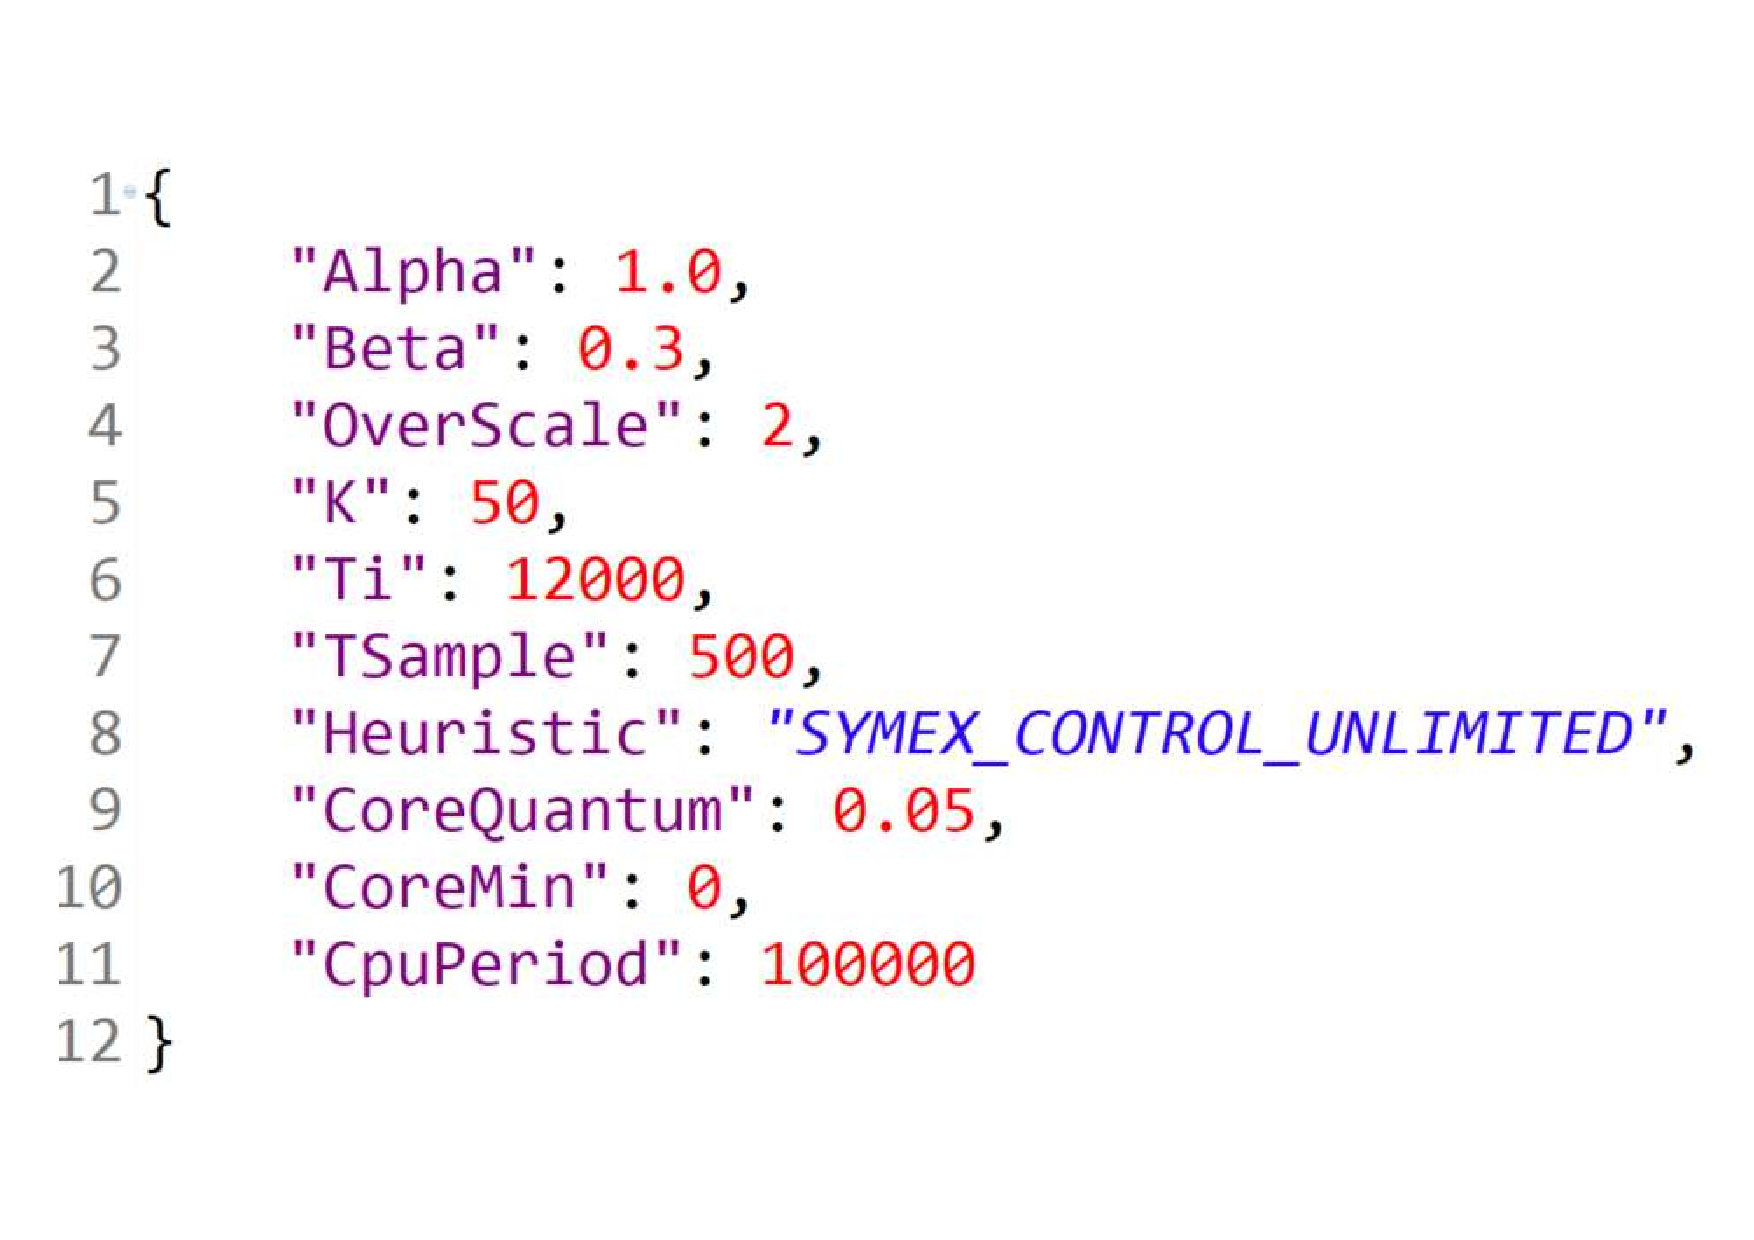
\includegraphics[width=\columnwidth]{images/xspark_symex_control_unlimited_parms.pdf}
	\caption{control.json \tool configuration parameters.}
	\label{fig:xSparkDagSymbConfigParms}
\end{figure}
\begin{figure}[thbp]
	\centering
	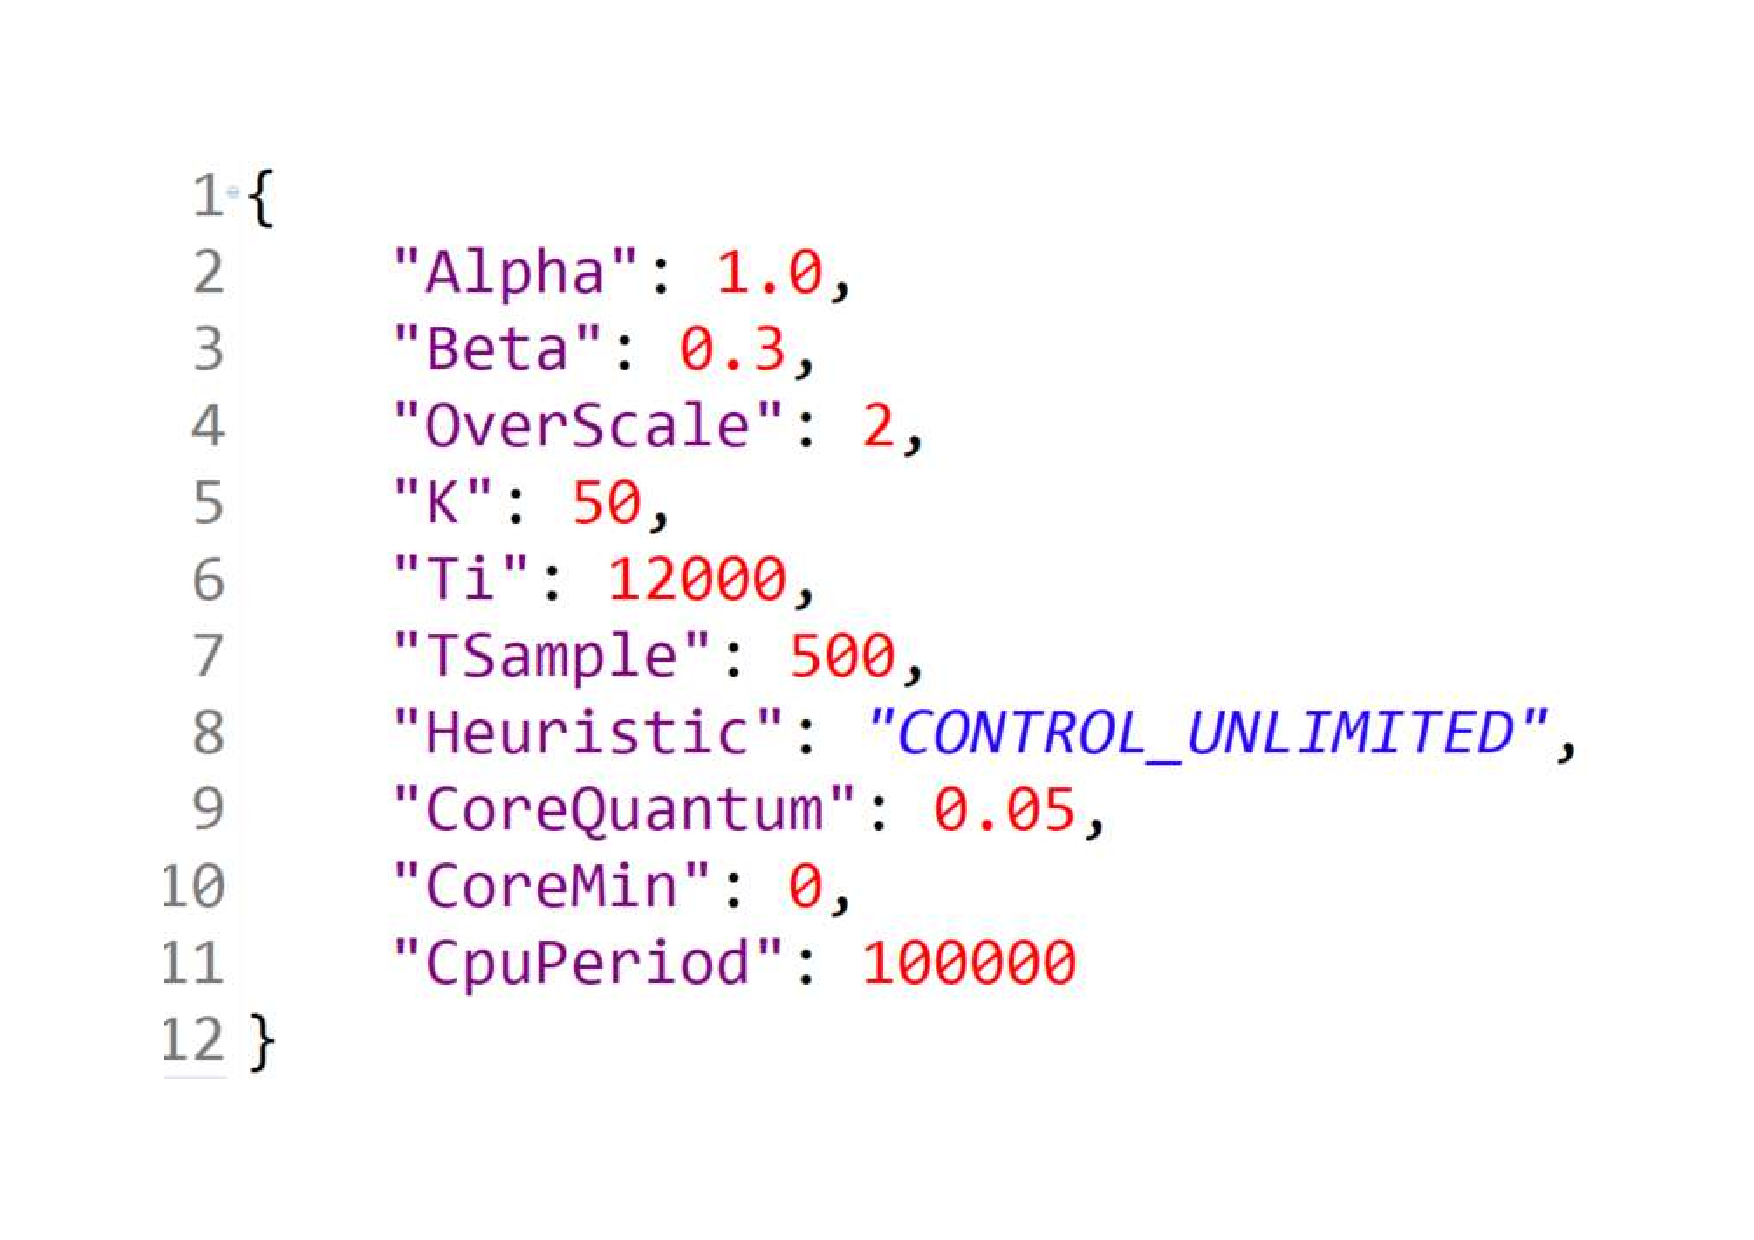
\includegraphics[width=\columnwidth]{images/xspark_control_unlimited_parms.pdf}
	\caption{control.json \cSpark configuration parameters.}
	\label{fig:xSparkConfigParms}
\end{figure}

\section{Tested Applications}\label{sec:tested_apps}
We performed the experiments with two applications: PromoCalls and Louvain.
PromoCalls is an example application that was developed at Politecnico di Milano in the Deib Labs\footnote{\url{https://github.com/seepep/promocalls}}.
It resembles a batch application from a telecommunications company that calculates promotional discounts based on the number of daily domestic and foreign calls (calls longer than a parametric threshold) made by customers. 
If a customer makes more than  $min_l$ local long calls or more than $min_a$ abroad long calls (or both) in a day, she may receive discounts on the calls made in that day, in the last $m$ months, or in the current month. 
Only some or all of the discounts may be applied to the customer depending on the possible combinations of the trigger conditions. 
PromoCalls uses Spark to efficiently analyze the data of all calls and calculate the applicable discounts.
PromoCalls was used as a reference application during the development of SEEPEP and for a preliminary assessment of the accuracy of the technique used.

Instead, to evaluate our approach to a real world application, we selected Louvain, a Spark implementation of the Louvain algorithm~\cite{Louvain} that we downloaded from a highly ranked GitHub repository\footnote{\url{https://github.com/Sotera/spark-distributed-louvain-modularity}}. Louvain uses \textit{GraphX}, a Spark library specialized for graph processing, suitable for representing large user networks and analyzing communities belonging to these networks.

\section{Experiments}\label{sec:experiments}
The experiments were performed on each of the applications subjected to the tests following the procedure described below, which consists of three distinct phases:
\begin{enumerate}[$1 $]
	\item Execution of \dSymb to obtain the path conditions and generate the launchers corresponding to each identified path.
	\item Profiling the application subject to the test with the launchers generated and obtaining the plans for each path.
	\item Use of tool to control the execution of the application by feeding it with input data sets larger by one order of magnitude compared to those used to generate the launchers.
\end{enumerate}
We have generated at least one large data set for each profiled path. We also set a reasonable deadline, that is $ 20\% $ longer than the minimum deadline, measured by running the application on Spark configured to use all the resources available on the clusters, and with the same data sets used in the experiments .

The datasets were randomly generated using \dSymb.

The comparison of \tool with the original \cSpark version has been done, for each application under test, identifying the best and worst cases, i.e. the paths with the lowest and highest number of stages\footnote{In case two paths have the same number of stages, we chose the path with the shortest/longest execution time  respectively for the best/worst case.}. In this way, we have quantified the error that \cSpark can generate due to the fact that it ignores which plan was used in the profiling phase.

\subsection{Results}
Results produced by\tool for PromoCalls and Louvain tools, up to the profiling phase, are shown in Tables~\ref{Table:Check:Promo} and ~\ref{Table:Check;Louvain}. Column $Path$ lists the paths found by \dSymb: $8$ unique paths were discovered in both cases. 

Column $Found?$ shows whether or not \dSymb succeeded in generating a test case (and thus a corresponding profiling launcher) for the identified paths: it was successful in generating test cases for all path of PromoCalls, instead it was able to identify 6 out of 8 possible paths of Louvain\footnote{The two paths of Louvain for which \dSymb was not successful in identifying a corresponding test case were manually inspected. In any case, the proof that either these paths are infeasible, or an input datasets can be identified that exercise these paths, is missing.}. As a matter of fact, we currently have no clue if Louvain can execute these program paths or not.)

Column $Jobs$ and column $Stages$ report  the number of jobs and stages collected when profiling the launchers with \cSpark, which range between 3 and 9 jobs, 3 and 9 stages for Promocalls, and 11 and 17 jobs, 73 and 364 stages for Louvain, respectively. These data are not available for the two paths of Louvain for which \dSymb did not generate a launcher.
In both tables, we marked with $^\bullet$ and $^\dagger$ the paths that correspond to the best and worst case, respectively, of each application. 

\begin{table}[thbp]
	\centering
	\hspace{1cm}
	\parbox{.48\linewidth}{
		%\hspace{0.1cm}
		\begin{tabular}{c|c|c|c}
			\toprule
			\multicolumn{1}{c|}{\textbf{Path}} &  \multicolumn{1}{c|}{\textbf{Found?}}   & \multicolumn{1}{c|}{\boldmath$\#Jobs$}  &  \multicolumn{1}{c}{\boldmath$\#Stages$}    \\
			%\rotatebox{90}{\textbf{Path}} &  
			%\rotatebox{90}{\textbf{Found?}}   & 
			%\rotatebox{90}{\boldmath$\#Jobs$}  &  %\rotatebox{90}{\boldmath$\#Stages$}    \\
			\midrule
			$0$ & Yes  & 6 & 6  \\	
			$1^{\bullet}$ & Yes  &  3 &  3 \\	
			$2$ & Yes & 7  & 7 \\
			$3$ & Yes &  6 & 6 \\
			$4$ & Yes & 8  & 8  \\
			$5$ & Yes & 7 & 7 \\
			$6^{\dagger}$ & Yes & 9 & 9 \\
			$7$ & Yes &  8 & 8 \\
			\bottomrule
		\end{tabular}
		\caption{\boldmath$PromoCalls$ paths.}
		\label{Table:Check:Promo}
	}
%\end{table}
%\begin{table}[thbp]
	\centering
	\parbox{.48\linewidth}{
		%	\vspace{0.78cm}
		\vspace{2cm}
		\hspace{0.5cm}
		\begin{tabular}{c|c|c|c|c}
			\toprule
			\multicolumn{1}{c|}{\textbf{Path}} &  \multicolumn{1}{c|}{\textbf{Found?}}   & \multicolumn{1}{c|}{\boldmath$\#Jobs$}  &  \multicolumn{1}{c}{\boldmath$\#Stages$}    \\
			%\rotatebox{90}{\textbf{Path}} &  
			%\rotatebox{90}{\textbf{Found?}}   & 
			%\rotatebox{90}{\boldmath$\#Jobs$}  &  %\rotatebox{90}{\boldmath$\#Stages$}    \\
			\midrule
			$0$ & Yes  &  11 & 149 \\	
			$1$ & Yes & 17 & 364  \\	
			$2^{\dagger}$ & Yes & 17 & 364 \\
			$3$ & Yes & 11  & 149  \\
			$4$ & No & - & - \\
			$5$ & No & -  & - \\	
			$6$ & Yes & 17 & 364 \\
			$7^{\bullet}$ & Yes & 8  & 73  \\		
			\bottomrule
		\end{tabular}
		\caption{\boldmath$Louvain$ paths.}
		\label{Table:Check;Louvain}
	}
	
\end{table}
\begin{table}[tbhp]
	\centering
	\begin{tabular}{r|c|c|c|c|c|c}
		%\toprule
		\multicolumn{1}{c|}{\textbf{Experiment}}   &
		%\multicolumn{1}{R{90}{1em}{|}}{\textbf{Experiment}} & \multicolumn{1}{c|}{\boldmath$deadline\,[s]$}  &  \multicolumn{1}{c|}{\boldmath$exec\_time\,[s]$}  & \multicolumn{1}{c|}{\boldmath$Violation$} &  \multicolumn{1}{c|}{\boldmath$error$}    & \multicolumn{1}{c|}{\boldmath$core\_alloc\,[\frac{core}{s}]$}  & \multicolumn{1}{c|}{\boldmath$penalty$}   \\
		%\rotatebox{90}{\textbf{Experiment}}   &
		\rotatebox{90}{\boldmath$deadline\,[s]$}  &  \rotatebox{90}{\boldmath$exec\_time\,[s]$}  & \rotatebox{90}{\boldmath$violation$} &  \rotatebox{90}{\boldmath$error$}    & \rotatebox{90}{\boldmath$core\_alloc\,[\frac{core}{s}]$}  & \rotatebox{90}{\boldmath$penalty$}   \\
		\midrule
		$xSpark_s$  & $91.4$   & $90.3$   & $N$   & $1.2\%$   & $41.3$   & $-$  \\
		$P_0 \,\,xSpark_w$  & $91.4$   & $88.0$   & $N$   & $3.8\%$   & $53.0$   & $28.3\%$  \\
		$xSpark_b$  & $91.4$   & $143.0$   & $Y$   & $56.4\%$   & $30.6$   & $\infty$  \\
		\midrule
		$xSpark_s$  & $56.4$   & $46.0$   & $N$   & $18.4\%$   & $56.2$   & $-$  \\
		$P_1 \,\,xSpark_w$  & $56.4$   & $45.3$   & $N$   & $19.6\%$   & $56.5$   & $0.5\%$  \\
		$xSpark_b$  & $56.4$   & $55.3$   & $N$   & $1.9\%$   & $38.2$   & $\text{-}33.6\%$  \\
		\midrule
		$xSpark_s$  & $107.8$   & $106.3$   & $N$   & $1.3\%$   & $39.2$   & $-$  \\
		$P_2 \,\,xSpark_w$  & $107.8$   & $104.0$   & $N$   & $3.5\%$   & $52.1$   & $32.9\%$  \\
		$xSpark_b$  & $107.8$   & $175.0$   & $Y$   & $62.4\%$   & $29.0$   & $\infty$  \\
		\midrule
		$xSpark_s$  & $87.5$   & $86.0$   & $N$   & $1.7\%$   & $42.4$   & $-$  \\
		$P_3 \,\,xSpark_w$  & $87.5$   & $83.0$   & $N$   & $5.1\%$   & $53.5$   & $26.2\%$  \\
		$xSpark_b$  & $87.5$   & $138.0$   & $Y$   & $57.8\%$   & $30.1$   & $\infty$  \\
		\midrule
		$xSpark_s$  & $147.6$   & $146.0$   & $N$   & $1.1\%$   & $37.0$   & $-$  \\
		$P_4 \,\,xSpark_w$  & $147.6$   & $130.0$   & $N$   & $11.9\%$   & $51.4$   & $38.9\%$  \\
		$xSpark_b$  & $147.6$   & $228.0$   & $Y$   & $54.5\%$   & $28.4$   & $\infty$  \\
		\midrule
		$xSpark_s$  & $77.0$   & $75.3$   & $N$   & $2.2\%$   & $41.0$   & $-$  \\
		$P_5 \,\,xSpark_w$  & $77.0$   & $70.0$   & $N$   & $9.1\%$   & $53.7$   & $30.9\%$  \\
		$xSpark_b$  & $77.0$   & $122.0$   & $Y$   & $58.4\%$   & $29.7$   & $\infty$  \\
		\midrule
		$xSpark_s$  & $122.2$   & $120.3$   & $N$   & $1.5\%$   & $39.2$   & $-$  \\
		$P_6 \,\,xSpark_w$  & $122.2$   & $120.7$   & $N$   & $1.2\%$   & $43.6$   & $11.3\%$  \\
		$xSpark_b$  & $122.2$   & $204.0$   & $Y$   & $67.0\%$   & $27.9$   & $\infty$  \\
		\midrule
		$xSpark_s$  & $112.1$   & $110.7$   & $N$   & $1.3\%$   & $39.2$   & $-$  \\
		$P_7 \,\,xSpark_w$  & $112.1$   & $100.0$   & $N$   & $10.8\%$   & $53.0$   & $35.2\%$  \\
		$xSpark_b$  & $112.1$   & $180.0$   & $Y$   & $60.6\%$   & $28.8$   & $\infty$  \\
		
		\bottomrule
	\end{tabular}
	\caption{Results for \boldmath$PromoCalls$}
	\label{Table:PerfPromo}
\end{table}


\begin{table}[htbp]
	\centering
	\begin{tabular}{r|c|c|c|c|c|c}
		%\toprule
		\multicolumn{1}{c|}{\textbf{Experiment}}   &
		%\multicolumn{1}{R{90}{1em}{|}}{\textbf{Experiment}} & \multicolumn{1}{c|}{\boldmath$deadline\,[s]$}  &  \multicolumn{1}{c|}{\boldmath$exec\_time\,[s]$}  & \multicolumn{1}{c|}{\boldmath$Violation$} &  \multicolumn{1}{c|}{\boldmath$error$}    & \multicolumn{1}{c|}{\boldmath$core\_alloc\,[\frac{core}{s}]$}  & \multicolumn{1}{c|}{\boldmath$penalty$}   \\
		%\rotatebox{90}{\textbf{Experiment}}   &
		\rotatebox{90}{\boldmath$deadline\,[s]$}  &  \rotatebox{90}{\boldmath$exec\_time\,[s]$}  & \rotatebox{90}{\boldmath$violation$} &  \rotatebox{90}{\boldmath$error$}    & \rotatebox{90}{\boldmath$core\_alloc\,[\frac{core}{s}]$}  & \rotatebox{90}{\boldmath$penalty$}   \\
		\midrule
		$xSpark_s$  & $184.3$   & $180.1$   & $N$   & $2.3\%$   & $35.9$   & $-$  \\
		$P_0 \,\,xSpark_w$  & $184.3$   & $142.0$   & $N$   & $23.0\%$   & $46.1$   & $28.4\%$  \\
		$xSpark_b$  & $184.3$   & $222.3$   & $Y$   & $20.6\%$   & $15.2$   & $\infty$  \\
		\midrule
		$xSpark_s$  & $228.0$   & $227.0$   & $N$   & $0.4\%$   & $32.3$   & $-$  \\
		$P_1 \,\,xSpark_w$  & $228.0$   & $222.0$   & $N$   & $2.6\%$   & $33.2$   & $2.8\%$  \\
		$xSpark_b$  & $228.0$   & $329.3$   & $Y$   & $44.4\%$   & $7.4$   & $\infty$  \\
		\midrule
		$xSpark_s$  & $292.8$   & $290.7$   & $N$   & $0.7\%$   & $32.3$   & $-$  \\
		$P_2 \,\,xSpark_w$  & $292.8$   & $289.0$   & $N$   & $1.3\%$   & $32.5$   & $0.5\%$  \\
		$xSpark_b$  & $292.8$   & $429.0$   & $Y$   & $46.5\%$   & $7.0$   & $\infty$  \\
		\midrule
		$xSpark_s$  & $228.7$   & $226.0$   & $N$   & $1.2\%$   & $35.5$   & $-$  \\
		$P_3 \,\,xSpark_w$  & $228.7$   & $211.3$   & $N$   & $7.6\%$   & $41.4$   & $16.6\%$  \\
		$xSpark_b$  & $228.7$   & $292.0$   & $Y$   & $27.7\%$   & $16.0$   & $\infty$  \\
		\midrule
		$xSpark_s$  & $163.0$   & $159.4$   & $N$   & $2.2\%$   & $38.4$   & $-$  \\
		$P_6 \,\,xSpark_w$  & $163.0$   & $158.0$   & $N$   & $3.0\%$   & $39.8$   & $3.8\%$  \\
		$xSpark_b$  & $163.0$   & $242.0$   & $Y$   & $48.5\%$   & $8.5$   & $\infty$  \\
		\midrule
		$xSpark_s$  & $156.0$   & $139.0$   & $N$   & $10.9\%$   & $33.2$   & $-$  \\
		$P_7 \,\,xSpark_w$  & $156.0$   & $131.5$   & $N$   & $15.7\%$   & $43.6$   & $31.4\%$  \\
		$xSpark_b$  & $156.0$   & $152.7$   & $N$   & $2.1\%$   & $30.9$   & $-7.0\%$  \\
		\bottomrule
	\end{tabular}
	\caption{Results for $Louvain$}
	\label{Table:Louvain}
	\vspace{-8mm}
\end{table}

The effectiveness of \tool to control the execution of the tested applications, whose inputs were fed with large datasets, is measured by the results of our experiments that are summarized in Tables~\ref{Table:PerfPromo} and ~\ref{Table:Louvain}. These tables also include the results obtained with the original version of \cSpark, tuned on the worst and best case datasets above, and allow us to compare \tool against \cSpark. The meaning of each column of the tables is explained here below.

For each profiled path $P_i$, column $Experiment$ indicates the data obtained with \tool ($xSpark_s$), and \cSpark configured with the worst-case dataset ($xSpark_w$) and with the best-case dataset ($xSpark_b$), respectively. 
In column $deadline$ we show the set deadline in seconds. 
In column $exec\_time$ the actual execution time of the application is reported in seconds, as the average of $5$ iterations of the experiments (for a total of $120$ executions of PromoCalls (8 paths $\times$ 5 repetitions $\times$ 3 modes) and $90$ executions of Louvain). 
In column $Violation$ we show the deadline violations (i.e., $exec_time > deadline$). 
The error  is quantified in column $error$, defined as:
%
\[
error = \frac{|deadline - exec\_time|}{deadline}\cdot100\%
\]
%
that is, the percentage change vs. the deadline of the distance between the actual execution time and the deadline itself. In general the smaller $error$, the more efficient is the resource allocation, provided that the deadline is not violated, since less resources were used to meet the goal. On the other hand, if the deadline is violated, to smaller errors correspond shorter delays. Note that if the deadline were to be considered strict, the penalty for a violation would be considered of infinite value~\cite{shin1994real}.
In column $core\_alloc$ we show the average core allocation during the execution, that is defined as:
%
\[
core\_alloc = \frac{\sum_{s = 0}^{exec\_time} coresAllocatedAtSecond(s)}{exec\_time} 
\]
%

We remark that the maximum value of $core\_alloc$ is $64$ core/second since $64$ is the number of cores provided by the cluster used for these experiments.

In the last column $penalty$ we quantify the performance of \tool compared to  \cSpark when executing the same experiment: $penalty$ is defined as:
\[
penalty = 
\begin{cases}
\frac{ru_{WORST|BEST}-ru_{SEEPEP}}{ru_{SEEPEP}}\cdot 100\%,& \text{if } Violation = No \\
\infty,              & \text{if } Violation = Yes
\end{cases}
\]

Remarkably in our experiments, \tool never violated the deadline, hence $penalty$ measures the amount of resources that either $xSpark_w$ or $xSpark_b$ have used with respect to \tool. E.g. a $penalty$ of 30\% means that \cSpark used 30\% more resources than \tool. Instead, a negative $penalty$ means that \cSpark used less  resources than \tool. Lastly, when the deadline is violated by either $xSpark_w$ or $xSpark_b$, we consider $penalty$ to be infinite~\cite{shin1994real}. 

As evidenced by the data in Tables~\ref{Table:PerfPromo} and ~\ref{Table:Louvain},  $xSpark_b$ violated the deadline in $7$ out of $8$ paths in the experiments with PromoCalls, and 5 out of 6 paths in the experiments with Louvain. This is due to the optimistic, yet wrong, estimations made in the profiling phase. To explain this behaviour, we have to consider that, for Promocalls, $xSpark_b$ computes the local deadlines and the resource allocation  as if the \plan always consisted of $3$ stages. As a consequence, in all the experiments but $P_1$ (which is the actual best-case path) \cSpark under allocates resources, resulting in the execution time eventually exceeding the deadline by as much as $51.9\%$. We measured the highest error displacement, equals to $67.0\%$, with the worst-case path $P_6$ where \cSpark faces the widest gap between the profiling estimations and the actual runtime workload. 

In the same tables we can appreciate that $xSpark_w$ does not violate any deadline, on the contrary it causes the earlier termination of the applications in most of the cases, with an $error$ between 1.2\% and 19.6\% in the case of PromoCalls, and between 1.3\% and 23\% in the case of Louvain. This beahoiur depends on the pessimistic, yet wrong, estimations made in the profiling phase,  that mistakenly consider the worst-case path of the applications to represent all the possible paths.
When considering paths $P_1$, $P_4$, $P_5$ and $P_7$ of PromoCalls,  and  $P_0$, $P_3$ and $P_7$ of Louvain, the error is greater than $7\%$, leading  to significantly sub-optimal resource allocations. 

Remarkably, and on the contrary, \tool does not violate any deadline and successfully provides an efficient resource allocation. The average error measured in our experiments is equal to $3.6\%$ for PromoCalls, where for $xSpark_b$ and $xSpark_w$ is $52.4\%$ and $8.1\%$, respectively, and equal to $2.9\%$ for Louvain, where $xSpark_b$ and $xSpark_w$ have an average error of $31.6\%$ and $8.9\%$, respectively.

The data in columns $core\_alloc$ confirm that \tool outperforms the performance of $xSpark_b$ and $xSpark_w$. $xSpark_b$ underestimates allocated resources so as to make \cSpark violate the deadlines in all experiments, except for path $P_1$ in PromoCalls and path $P_7$ in Louvain (the best cases). In the latter two cases, profiled data match the runtime workload, leading $xSpark_b$ to outperform both $xSpark_w$ and \tool, and minimizes the error and used resources. 

\tool allocates an average of $25.5\%$ fewer resources in PromoCalls, and $13.9\%$ in Louvain, with respect to $xSpark_w$.

From the results of our experiments we can evince a positive answer to both research questions $RQ_1$ and $RQ_2$, because \tool effectively and efficiently controls the allocation of resources during the execution of PromoCalls and Louvain, keeping the execution times within considered deadlines with significantly smaller errors and consuming a lower amount of resources than the original version of \cSpark.

\section{Threats to Validity}
\label{sec:ThreatsToValidity}

We came up with a considerable trial effort, which has led us to perform a total of $226$ experiments on two different applications: a paradigmatic example and a real-world application taken from GitHub. We have shown that \dSymb was able to find a test-case for 14 out 16 of the application paths statically identified with symbolic execution, and demostrated how \cSpark could take advantage from the integration with \dSymb. In this section, we highlight the threats that may constrain the validity of our current results~\cite{wohlin2006empirical}:

\textbf{Internal Threats}.  The test cases generated by \dSymb have been slightly modified to increase the size of the datasets (without breaking the path conditions) for the execution of the experiments. This was done to ensure that we could test the desired paths and reliably obtain different repetitions of the experiments. However, data sets were not created in a totally random way. For this reason, we have preliminary executed some experiments with completely randomly created data sets and have obtained a similar result to the one presented.
A broader set of experiments could be done to address this aspect as a matter for future developments.

\textbf{External Threats}. A limit to the generality of the experiments and of the solutions tested may derive from the assumption underlying the choice of the Spark applications that we have considered. We have chosen two applications: one that uses Spark's core transformations and one that uses the \textit{GraphX} entry for graph analysis. To increase the degree of generality of evaluations, an extension of the number and variety of Spark applications is desirable, taking into consideration different types, such as those that exploit machine learning solutions and use SQL.

Profiling as it is currently done constitutes an additional limitation of the approach used. In fact, a profiling session is required for each test case (launcher) found by \dSymb, but this could become a problem when the number of program paths becomes too high. A desirable direction for a future work could be the improvement of this part of the tool chain. The improvement could be achieved through the adoption of a branch-based criterion to select profiling executions, replacing the current path-based criterion. The underpinning rationale is that since the execution of all the program branches assures that any possible \plan of the program has been profiled at least once; ; then, after profiling, we can map the profiled \plans on the paths (and then the path conditions) that include the corresponding program branches. This optimization might also mitigate the issues with paths that our test generator fails to exercize, such as the 2 uncovered paths that we experienced in Louvain.

\textbf{Concept and Conclusion Threats}. The experiments demonstrate the validity of our idea, namely that the knowledge of the different \plans generated by the Spark applications helps to analyze and control their performance and execution time. Furthermore, we show that an approach based simply on knowledge of the worst case may be sufficient to limit the number of deadline violations, but is significantly less efficient than the one we obtain with our solution. The results obtained are statistically robust and they show only a small variance. 
 
	\chapter{Conclusion} \label{chap:conclusion}
%\begin{flushright}{\slshape    
%   Science, my boy, is made up of mistakes, but they are mistakes
%   which it is useful to make, because they lead little by little
%   to the truth}. \\ \medskip --- \citeauthor{verne_journey:1957}
%   \citetitle{verne_journey:1957} \citeyear{verne_journey:1957}
%\end{flushright} 
\lettrine[lines=4]{\textcolor{purple}{I}}{n} the previous chapters we have presented the work done in order to support deadline-based \qos constrained multi-\plan Spark applications, i.e. applications whose execution flow cannot be represented with a single \textit{Parallel Execution Plan} (\plan), and whose actual execution flow is only known at runtime. 

This chapter summarizes the conclusion of our work and the future works to improve the solution by extending the field of applicability and optimizing each  individual components, to obtain a more complete and efficient solution.

%\section{Conclusion}\label{sec:conclusion}

%In order to overcome the current limitation that requires Spark applications to be represented by a single \plan at runtime, this thesis presented \tool, a solution based on a lightweight symbolic execution of the target application to extract the family of \plans that is used to generate a set of profiles of the application, that is used to tune xSpark to adapt its runtime dynamic resource allocation to help meet a user-defined application deadline.

The contribution provided by this thesis consists of the design and the development of \tool, a solution composed by 

1 -- an original and lightweight application of the principles of symbolic execution to detect the parallel plans of the execution of Spark multi-\plan applications and  create the related execution profiles, 

2 -- the integration in xSpark of additional features that exploit the knowledge of the execution plans to manage the allocation of resources at runtime to help achieve the goal of maintaining the execution time of the application within a deadline specified by the user, and 

3 -- the development of a \textit{Python tool} to automate the entire testing lifecycle, including the application profiling, the test execution and reporting of test results. 

The results if the evaluation show that \tool meets all the expectations identified by the research questions formulated in \MySec{sec:solution_contribution}, as it misses fewer deadlines and allocate resources more efficiently than \cSpark. 

%\section{Future Work}\label{sec:future_work}
%As the applicability of the profiling contained in \tool is currently subject to the limitation related to the number of paths to be profiled, that requires the profiling of the entire application by a specific launcher for each path identified by \dSymb, and can become practically unfeasible if the number of paths is too high, a desirable future work could be directed at improving this part of the tool chain. This future work would be focused to moving away from the current profiling phase which uses path-based selection criteria in favour of a profiling  that uses branch-based criteria. 
 
%Another future work could consist in the research along the lines of the applicability of the proposed solution to execute non-strict deadlines QoS-constrained multi-\plan applications.
Since the current solution focuses on controlling a single application, a future work could be directed at extending \tool to control multiple concurrent applications.

 
	
	% ************************************************************
	% Backmatter
	%*************************************************************
	\cleardoublepage%********************************************************************
% Bibliography
%*******************************************************
% work-around to have small caps also here in the headline
\manualmark
\markboth{\spacedlowsmallcaps{\bibname}}{\spacedlowsmallcaps{\bibname}}
%\phantomsection 
\refstepcounter{dummy} 
% to have the bib a bit from the rest in the toc
\addtocontents{toc}{\protect\vspace{\beforebibskip}}
\addcontentsline{toc}{chapter}{\tocEntry{\bibname}}
\label{app:bibliography} 
\printbibliography
	%\appendix
	% \cleardoublepage\part{Appendix}
	%%********************************************************************
% Appendix
%*******************************************************
% If problems with the headers: get headings in appendix etc. right
\markboth{\spacedlowsmallcaps{Appendix}}{\spacedlowsmallcaps{Appendix}}
%************************************************
\chapter{Appendix example: code listings}

%\begin{flushright}{\slshape    
%    We have seen that computer programming is an art, \\ 
%    because it applies accumulated knowledge to the world, \\ 
%    because it requires skill and ingenuity, and especially \\
%    because it produces objects of beauty.} \\ \medskip
%    --- \citeauthor{knuth:1974}, \citetitle{knuth:1974},
%\citeyear{knuth:1974} 
%\end{flushright}

\section{The \texttt{listings} package to include source code}
Source code is usually not part of the text of a thesis, but if it is an original contribution it makes sense to le the code speak by itself instead of describing it. The package \verb!listings! provide the proper layout tools. Refer to its manual if you need to use it, an example is given in listing \ref{lst:probCounter}.

\lstinputlisting[
	firstline=1,
	lastline=47,
	float=tb,
	language=C++,
	tabsize=2,
	numbers=left,
	numberstyle=\tiny,
	stepnumber=2,
	numbersep=5pt,
	caption={Code snippet with the recursive function to evaluate the pdf of the sum $Z_N$ of $N$ random variables equal to $X$.}, 
	captionpos=t,
	label=lst:probCounter
	]{CodeFiles/probabilityCounter.cpp}

\end{document}
% ****************************************************************